% -*- Mode:TeX -*-

%% IMPORTANT: The official thesis specifications are available at:
%%            http://libraries.mit.edu/archives/thesis-specs/
%%
%%            Please verify your thesis' formatting and copyright
%%            assignment before submission.  If you notice any
%%            discrepancies between these templates and the 
%%            MIT Libraries' specs, please let us know
%%            by e-mailing thesis@mit.edu

%% The documentclass options along with the pagestyle can be used to generate
%% a technical report, a draft copy, or a regular thesis.  You may need to
%% re-specify the pagestyle after you \include  cover.tex.  For more
%% information, see the first few lines of mitthesis.cls. 

%\documentclass[12pt,vi,twoside]{mitthesis}
%%
%%  If you want your thesis copyright to you instead of MIT, use the
%%  ``vi'' option, as above.
%%
%\documentclass[12pt,twoside,leftblank]{mitthesis}
%%
%% If you want blank pages before new chapters to be labelled ``This
%% Page Intentionally Left Blank'', use the ``leftblank'' option, as
%% above.

%\documentclass[12pt,twoside,doublespace]{mitthesis}
\documentclass[12pt,twoside,singlespace]{mitthesis}

\usepackage{algorithm}                  % for describing algorithms nicely
\usepackage[noend]{algpseudocode}
\usepackage{amsmath}
\usepackage{amssymb}
\usepackage{amsthm}                     % \newtheorem (conflicts with llncs template due to \proof)
\usepackage[english]{babel}
\usepackage{booktabs}                   % for table spacing, \midrule
%% These have been added at the request of the MIT Libraries, because
%% some PDF conversions mess up the ligatures.  -LB, 1/22/2014
\usepackage{calculator}
\usepackage{cfr-lm} % \textsi for small-caps italics
\usepackage{cite}
\usepackage{cmap}
\usepackage{epigraph}
\usepackage{enumitem}
\usepackage[T1]{fontenc}
\usepackage{forest}
\usepackage{graphicx}
\usepackage[hidelinks]{hyperref}        % Use [draft] to fix "\pdfendlink ended up in different 
\usepackage{hyphenat}
\usepackage[utf8]{inputenc}
\usepackage[margin=1in]{geometry}
\usepackage{lgrind}
\usepackage[babel=true]{microtype}
\usepackage{lmodern}
\usepackage{makecell}                   % use \makecell{text\\ new line} to break up lines inside table cells
\usepackage{mathtools}                  % for \DeclarePairedDelimiter{\ceil}{\lceil}{\rceil}
\usepackage{multirow}
\usepackage{pdflscape}                  % for rotating PDF pages
%\usepackage{refcheck}                  % prints "unused bibitem" in the build log for unused citations. WARNING: Also annotates PDF to indicate what's been unreferenced.
\usepackage{rotating}
\usepackage{tocloft}
\usepackage{xcolor}
\usepackage{xspace}
\usepackage{xstring}                    % for \IfStrEqCase

\pagestyle{plain}
\setcounter{secnumdepth}{3}
\setcounter{tocdepth}{3}

% global spacing for itemize lists
\setitemize{noitemsep,topsep=5pt,parsep=3pt,partopsep=1pt}

%
% WARNING: Keep here due to LaTeX bugs
%
\usepackage[noabbrev,capitalize]{cleveref}            % WARN: Must come after hyperref
\usepackage[caption=false, font=footnotesize]{subfig} % WARN: When moved up in the sorted list, getting "TeX capacity exceeded, sorry [input stack size=5000]" error

\newcommand{\mytitle}{How to Keep a Secret and Share a Public Key\\(Using Polynomial Commitments)}

\newif\ifCameraReady
\CameraReadytrue % camera-ready
\newif\ifHideAcks
%\HideAckstrue % hides acks and quote

%
% Some colors:
%  Blue: #268bd2
%  (Grey) Blue: #657b83
%  Green: #859900
%  (Dark) Orange: #cb4b16
%  Red: #dc322f
%  Periwinkle: #6c71c4
%  Pink: #d33682
%  Teal: #2aa198
%  Yellow: #b58900
%
\definecolor{myBlueColor}{HTML}{268BD2}
\definecolor{myYellowColor}{HTML}{B58900}
\definecolor{myGreenColor}{HTML}{859900}
\definecolor{myRedColor}{HTML}{DC322F}
\newcommand{\myblue}[1]{\textcolor{myBlueColor}{#1}}
\newcommand{\myred}[1]{\textcolor{myRedColor}{#1}}
\newcommand{\red}[1]{\textcolor{red}{#1}}
\newcommand{\myyellow}[1]{\textcolor{myYellowColor}{#1}}
\newcommand{\mygreen}[1]{\textcolor{myGreenColor}{#1}}

\newcommand{\alice}{Alice\xspace}
\newcommand{\bob}{Bob\xspace}

%
% Markup defs
%
%\newcommand{\xmark}{\ding{55}}
\newcommand{\api}{\hangindent=\parindent \hangafter=1 \noindent}
\newcommand{\comment}[1]{}

%
% Some mathy things
%

\DeclareMathOperator{\dom}{Dom}    % domain of a function
\DeclareMathOperator{\Ima}{Im}	% image of a function
\DeclareMathOperator*{\argmin}{argmin}
\DeclarePairedDelimiter{\ceil}{\lceil}{\rceil}
\DeclarePairedDelimiter{\floor}{\lfloor}{\rfloor}

\newcommand{\Group}{\mathbb{G}}
\newcommand{\GroupHidOrd}{\ensuremath{\Group_{\textbf{?}}}}
\newcommand{\Fp}{\mathbb{F}_p}
\newcommand{\GT}{\mathbb{G}_T}
\newcommand{\Z}{\mathbb{Z}}
\newcommand{\Zp}{\mathbb{Z}_p}
\newcommand{\ZN}{\mathbb{Z}_N}
\newcommand{\ZNstar}{\mathbb{Z}_N^*}
\newcommand{\QRN}{\mathbb{QR}_N}
% prime (known) order (PO) group setup algorithm
\newcommand{\groupkosetup}{\ensuremath{\mathcal{G}_{\mathsf{prime}}}}
% hidden-order (HO) group setup algorithm
\newcommand{\grouphosetup}{\ensuremath{\mathcal{G}_{\mathsf{hidden}}}}

\newcommand{\primes}{\ensuremath{\mathsf{Primes}}}
\newcommand{\poly}{\mathsf{poly}}
\newcommand{\negl}{\mathsf{negl}}
\newcommand{\nonnegl}{\eta}
\newcommand{\Hb}{\mathcal{H}}                       % hash function to binary string
\newcommand{\Hp}{\mathcal{H}_{\mathbb{F}}}          % hash function to finite field
\newcommand{\Hprime}{\mathcal{H}_{\mathsf{prime}}}   % hash to primes

\newcommand{\bezout}{B\'ezout\xspace}
\newcommand{\Ell}{\mathcal{L}}
\newcommand{\Adv}{\ensuremath{\mathcal{A}}\xspace} % adversary
\newcommand{\AdvB}{\ensuremath{\mathcal{B}}\xspace} % adversary

\theoremstyle{definition}
\newtheorem{definition}{Definition}[section]
\newtheorem{theorem}{Theorem}[section]
\newtheorem{corollary}{Corollary}[theorem]
\newtheorem{lemma}[theorem]{Lemma}

%
% Accumulators (RSA) notation
%

%
% Po(K)E protocols
%
\newcommand{\poe}{PoE\xspace}
\newcommand{\pokestar}{PoKE$^*$\xspace}
\newcommand{\poke}{PoKE\xspace}
\newcommand{\poketwo}{PoKE2\xspace}

%
% Polynomial commitment APIs
%
\newcommand{\vk}{\ensuremath{\mathsf{VK}}\xspace}
\newcommand{\PPsdh}{\ensuremath{\mathsf{PP}^\mathsf{SDH}}\xspace}
\newcommand{\PPpke}{\ensuremath{\mathsf{PP}^\mathsf{PKE}}\xspace}
\newcommand{\pp}{\ensuremath{\mathsf{pp}}\xspace}
\newcommand{\nizkpok}{\ensuremath{\pi^\mathsf{DLog}}\xspace}
\newcommand{\kzgbatchproof}{\ensuremath{\pi^\mathsf{batch}}\xspace}
\newcommand{\polysetup}{\ensuremath{\mathsf{Poly.Setup}}\xspace}
\newcommand{\polycommit}{\ensuremath{\mathsf{Poly.Commit}}}
\newcommand{\polyopen}{\ensuremath{\mathsf{Poly.Open}}}
\newcommand{\polyverifypoly}{\ensuremath{\mathsf{Poly.VerifyPoly}}}
\newcommand{\polycreatecommwitness}{\ensuremath{\mathsf{Poly.CreateCommWitness}}}
\newcommand{\polycreatewitness}{\ensuremath{\mathsf{Poly.ProveEval}}\xspace}
\newcommand{\polyverifyeval}{\ensuremath{\mathsf{Poly.VerifyEval{\xspace}}}}
\newcommand{\polyverifycommittedeval}{\ensuremath{\mathsf{Poly.VerifyCommEval}}}
\newcommand{\polycombinecomms}{\ensuremath{\mathsf{Poly.CombineComms}}}

\newcommand{\decominfo}{\ensuremath{\delta}\xspace}

%
% Commands for describing algorithms
%
\newcommand*\Let[2]{\State #1 $\gets$ #2}
\newcommand{\emptyline}{\State}
\newcommand{\AssertStateless}{\textbf{assert}\xspace}
\newcommand{\Assert}{\State \AssertStateless}
\algnewcommand{\LineComment}[1]{\State \(\triangleright\) #1}

%
% Notations for trees and forests
%
\newcommand{\prefixes}{\ensuremath{\mathsf{P}}}
\newcommand{\parent}{\ensuremath{\mathsf{parent}}}
\newcommand{\leaves}{\ensuremath{\mathsf{leaves}}}
\newcommand{\internal}{\ensuremath{\mathsf{internal}}}
\newcommand{\rootnode}{\ensuremath{\mathsf{root}}}
\newcommand{\bin}{\ensuremath{\mathsf{bin}}}
\newcommand{\roots}{\ensuremath{\mathsf{roots}}}
\newcommand{\sibling}{\ensuremath{\mathsf{sibling}}}
\newcommand{\treepath}{\ensuremath{\mathsf{path}}}
\newcommand{\isancestor}{\ensuremath{\mathsf{isAncestor}}}
\newcommand{\isrightchild}{\ensuremath{\mathsf{isRightChild}}}

%
% Markups for to do's and notes
%
\mathchardef\mhyphen="2D % Hyphens in math mode: https://www.logic.at/staff/salzer/etc/mhyphen/
\newcommand{\authnote}[2]{{\textcolor{red}{{#1: }\textcolor{blue}{ #2}}}}


\ifCameraReady
    \newcommand{\anote}[1]{}
    \newcommand{\snote}[1]{}
\else
    \newcommand{\anote}[1]{{\authnote{Alin}{#1}}}
    \newcommand{\snote}[1]{{\authnote{Srini}{#1}}}
\fi

\newcommand{\upperbound}{\ensuremath{B}\xspace}

%
% Scheme names
%
\newcommand{\biaas}{\ensuremath{\mathsf{AAS}_\mathsf{bilinear}}\xspace}
\newcommand{\biaad}{\ensuremath{\mathsf{AAD}_\mathsf{bilinear}^{\mathsf{tall}}}\xspace}
\newcommand{\biaadset}{\ensuremath{\mathsf{AAD}_\mathsf{bilinear}^{\mathsf{short}}}\xspace}

\newcommand{\rsaaas}{\ensuremath{\mathsf{AAS}_\mathsf{rsa}}\xspace}
\newcommand{\rsaaad}{\ensuremath{\mathsf{AAD}_\mathsf{rsa}^{\mathsf{tall}}}\xspace}
\newcommand{\rsaaadset}{\ensuremath{\mathsf{AAD}_\mathsf{rsa}^{\mathsf{short}}}\xspace}

%
% Helpful terminology that might change later
%
\newcommand{\communionTree}{Communion Tree\xspace}
\newcommand{\communionTrees}{Communion Trees\xspace}
\newcommand{\prefixCommunionTree}{Prefix Communion Tree\xspace}
\newcommand{\prefixCommunionTrees}{Prefix Communion Trees\xspace}
\newcommand{\frontierCommunionTree}{Frontier Communion Tree\xspace}
\newcommand{\frontierCommunionTrees}{Frontier Communion Trees\xspace}

%
% Append-only Auth. Set/Dictionary API
%
\newcommand{\setup}{\ensuremath{\mathsf{Setup}}\xspace}

\newcommand{\append}{\ensuremath{\mathsf{Append}}\xspace}
\newcommand{\multiappend}{\append^{+}}

\newcommand{\proveappendonly}{\ensuremath{\mathsf{ProveAppendOnly}}\xspace}
\newcommand{\verappendonly}{\ensuremath{\mathsf{VerAppendOnly}}\xspace}

% AAS-specific
\newcommand{\provememb}{\ensuremath{\mathsf{ProveMemb}}\xspace}
\newcommand{\vermemb}{\ensuremath{\mathsf{VerMemb}}\xspace}

% AAD-specific
\newcommand{\provelookup}{\ensuremath{\mathsf{ProveLookup}}\xspace}
\newcommand{\verlookup}{\ensuremath{\mathsf{VerLookup}}\xspace}

%
% Algorithms
%
\newcommand{\verpath}{\ensuremath{\mathsf{VerPath}}\xspace}
\newcommand{\provepath}{\ensuremath{\mathsf{ProvePath}}\xspace}
\newcommand{\proverootaccs}{\ensuremath{\mathsf{ProveRootAccs}}\xspace}
\newcommand{\provefrontier}{\ensuremath{\mathsf{ProveFrontier}}\xspace}
\newcommand{\verfrontier}{\ensuremath{\mathsf{VerFrontier}}\xspace}
\newcommand{\accumulate}{\ensuremath{\mathsf{Accum}}\xspace}
\newcommand{\createfrontier}{\ensuremath{\mathsf{CreateFrontier}}\xspace}

%
% Variables used in AAS algorithms
%
\newcommand{\elems}{\myblue{\mathbf{S}}}                     % notation for the set of elements at a certain node in the forest
\newcommand{\hash}{\myblue{\mathbf{h}}}                      % notation for Merkle hash in the forest
\newcommand{\acc}{\myblue{\mathbf{a}}}                       % notation for node accumulator commitment: \acc = g^{\accpoly(s)}
\newcommand{\eacc}{\myblue{\hat{\mathbf{a}}}}                % for extractable counterpart of \eacc
\newcommand{\subsetProof}{\myblue{\boldsymbol{\pi}}}
\newcommand{\bft}{\myblue{\boldsymbol{\sigma}}}              % notation for frontier accumulator commitment (on the server side): \fac = g^{\fropoly(s)}
\newcommand{\disj}{\myblue{\boldsymbol{\psi}}}               % notation for disjointness witness between a node accumulator and a frontier accumulator

% Not global variables
\newcommand{\charpoly}{\mathcal{C}}                 % characteristic polynomial of a set
\newcommand{\accpoly}{\alpha}                       % notation for node accumulator polynomial
\newcommand{\fropoly}{\phi}                         % notation for frontier accumulator 
\newcommand{\fac}{o}                                % notation for frontier accumulator commitment (on the verifier side): \fac = g^{\fropoly(s)}
\newcommand{\efac}{\hat{o}}                         % for extractabile counterpart of \fac
\newcommand{\CP}{\chi}                              % completeness proof w.r.t. frontier accumulator

%
% Notation for AAS/AAD
%
\newcommand{\AS}{\mathcal{S}}       % authenticated set
\newcommand{\AD}{\mathcal{D}}       % authenticated dictionary

%
% Names for our schemes
%
\newcommand{\jfdkg}{\ensuremath{\mathsf{JF}}-\ensuremath{\mathsf{DKG}}\xspace}   % Gennaro et al. abstraction for Pedersen's DKG
\newcommand{\newdkg}{\ensuremath{\mathsf{New}}-\ensuremath{\mathsf{DKG}}\xspace} % Gennaro et al. DKG with Pedersen commitments and Feldman-verification for reconstruction of g^{z_i}'s
\newcommand{\ejfdkg}{\ensuremath{\mathsf{eJF}}-\ensuremath{\mathsf{DKG}}\xspace} % Kate's DKG with PolyCommit
\newcommand{\evss}{\ensuremath{\mathsf{eVSS}}\xspace}

\newcommand{\ourvss}{\ensuremath{\mathsf{AMT}} \ensuremath{\mathsf{VSS}}\xspace}
\newcommand{\ourdkg}{\ensuremath{\mathsf{AMT}} \ensuremath{\mathsf{DKG}}\xspace}  % Our DKG protocol


%% WARNING: Used both as the AMT VSS/DKG dealer complexity and as the time to compute a multipoint evaluation.
\newcommand{\amtDealTime}{\ensuremath{n\log{t}}\xspace}
\newcommand{\amtOneShareVerifTime}{\ensuremath{\log{t}}\xspace}
%% WARNING: Used both as the time to verify all shares, as the # of pairings computed during verification and as the communication complexity required to send all shares.
\newcommand{\amtAllShareVerifTime}{\ensuremath{n\log{t}}\xspace}
%% Proof size for AMT on poly of deg t-1 evaluated at n > t points is 1 + \log2floor(t-1)
\newcommand{\amtProofSize}[1]{\ensuremath{\floor{\log{(#1-1)}} + 1}\xspace}
%
% Vector Commitment API
%
\newcommand{\vcsetup}{\ensuremath{\mathsf{VC.Setup}}}
\newcommand{\vccommit}{\ensuremath{\mathsf{VC.Commit}}}
\newcommand{\vcopen}{\ensuremath{\mathsf{VC.Open}}}
\newcommand{\vcverify}{\ensuremath{\mathsf{VC.Verify}}}
\newcommand{\vcupdate}{\ensuremath{\mathsf{VC.Update}}}
\newcommand{\vcproofupdate}{\ensuremath{\mathsf{VC.ProofUpdate}}}


% Performance numbers for BLS/VSS/DKG
\input{perf}

%% This bit allows you to either specify only the files which you wish to
%% process, or `all' to process all files which you \include.
%% Krishna Sethuraman (1990).
%%
%% ...but I removed them because I didn't find them useful. Alin Tomescu (2015).

%\typein [\files]{Enter file names to process, (chap1,chap2 ...), or `all' to
%process all files:}
%\def\all{all}
%\ifx\files\all \typeout{Including all files.} \else \typeout{Including only \files.} \includeonly{\files} \fi

\begin{document}

\include{cover}

% Some departments (e.g. 5) require an additional signature page.  See
% signature.tex for more information and uncomment the following line if
% applicable.
% \include{signature}
\pagestyle{plain}

%
% Table of contents
%
\include{contents}

% List of figures and tables (which no one reads, I presume)
\ifCameraReady
\cleardoublepage
\listoffigures
\cleardoublepage
\listoftables
\fi

%%%%%%%%%%%%%%%%%%%
% Thesis chapters %
%%%%%%%%%%%%%%%%%%%

%
% Part 0: Intro
%

    \chapter{Introduction}
    \section{How to Share a Public Key}
\label{s:intro:part1}

Almost every cryptographic scheme assumes actors know each other's public keys.
This assumption is often referred to as the \textit{public key infrastructure} (PKI) assumption.
For example, a PKI enables users to safely shop online on Amazon.com, to message each other securely on WhatsApp, and to use social media on LinkedIn.com.
Yet, despite their absolute necessity for security, state of the art PKIs remain inadequate in several ways.

First, PKIs rely on the unreasonable assumption of \textit{trusted parties}.
For example, Facebook, who develops and owns WhatsApp, runs a \textit{public key directory} (PKD) mapping each user's phone number to that user's public key.
This \textit{centralized} control of the PKD by Facebook is quite natural. 
After all, the PKD is a crucial component of WhatsApp's infrastructure and needs incentives to be maintained, incentives which Facebook has.
Unfortunately, this centralized approach assumes we live in a world where Facebook cannot be compromised or coerced.
In reality, mass surveillance revelations tell us the exact opposite story~\cite{EdSnowden,AAB+15}.
Thus, it is not unfathomable for a rogue Facebook to \textit{man-in-the-middle} ``secure'' WhatsApp conversations.
Indeed, this would not be too difficult either.
To snoop on two users, say \textit{\alice} and \textit{\bob}, Facebook need only \textit{equivocate} about their public keys in the PKD.

Second, when trusted parties go rogue, \textit{PKI attacks cannot be easily detected by victims} like Alice and Bob.
We focus on ``detection'' rather than ``prevention,'' since it is impossible to prevent PKI attacks in this strong, pessimistic model where trusted parties can go rogue.
Fortunately, post-attack detection is still possible, although not always easily achieved, as we detail next.

Consider the following (rather contrived) example.
\alice and \bob's WhatsApp conversation is man-in-the-middled by Facebook.
Fortunately, they both ``record'' all of their encrypted WhatsApp traffic.
They then meet in a coffee shop, inspect this traffic and notice that, at some point, their public keys were changed to unrecognized \textit{fake} ones that were subsequently used to encrypt their messages.
% Bob notices in Alice's recorded traffic that his public key was changed.
% Alice notices in Bob's traffic that her public key was changed too.
They then conclude a man-in-the-middle attack occurred.
However, their effort is considerable and does not scale to detecting attacks in multiple conversations.
Thus, more efficient detection methods are needed.

Third, (some) PKIs suffer from a \textit{weakest link in the chain} problem.
In other words, while one trusted party is an unreasonable assumption, $n>1$ trusted parties is much worse, since it increases the attack surface.
Sadly, the PKI used to secure HTTPS connections is the best example of this.
The \textit{Web PKI} is comprised of $1400$+ \textit{Certificate Authorities} (CAs)~\cite{ssliverse-talk} which digitally sign \textit{certificates} that map a website to its public key.
Quite terrifyingly, \textit{any} CA, in \textit{any} country, can sign a certificate for \textit{any} website.
Not surprisingly, this has led to many websites being surreptitiously \textit{impersonated}~\cite{cahacks,cahacksurvey}.
Even worse, it is conceivable that some impersonation attacks went undetected.
Fortunately, in 2013, Google took a key step towards \textit{detecting} and thus \textit{deterring} such attacks~\cite{ct}, which we discuss next.

\paragraph{Maintaining Trust in PKIs with Transparency Logs.}
In 2011, Google was the victim of two impersonation attacks~\cite{mitmgoogle,mitmgoogle2}.
As a result, in March 2013, Google deployed \textit{Certificate Transparency} (CT)~\cite{ct} as a way of detecting impersonation attacks and, hopefully, deterring them by publicly (though not provably) revealing their traces.
The key idea behind CT is to \textit{require} that all certificates for websites be published in a \textit{transparency log}.
In other words, unless a certificate comes with an \textit{inclusion proof} in the transparency log, a browser such as Firefox will never accept that certificate.
This way, if a rogue CA issues a fake certificate for a victim website, then the victim can detect this attack by searching or \textit{monitoring} in the transparency log.
This immediately raises the question of who runs this log and what if, just like a CA, it misbehaves?
The answer is an untrusted \textit{log server} runs the log but, if it misbehaves, it can be caught either (1) by \textit{domain owners}  such as \texttt{google.com},  \texttt{yahoo.com} or \texttt{your-website.com}, or (2) by users like \alice and \bob, or (3) by any other third-party \textit{verifier}.
Importantly, this misbehavior can be \textit{cryptographically proven}.

It is important to understand that CT logs cannot \textit{prevent} impersonation attacks, since a rogue CA can always (``kamikaze-style'') publish a fake certificate for, say, \texttt{google.com} in the log which will be used by (unsuspecting) users, until the fake certificate is detected and revoked by Google.
Instead, CT logs make such attacks quickly \textit{detectable} by the impersonated victim.
Specifically, the victim can now search the log for its certificates (i.e., monitor) and discover the fake certificate.
Unfortunately, this does not prove the certificate is ``fake.''
After all, the CA can falsely claim the victim was the one who asked for this certificate to be issued.
Since there is no cryptographic way of figuring out the truth, this must be resolved in the real world via the judicial system.
This way, incompetent or malicious CAs can be eliminated from the Web PKI, leading to a more trustworthy ecosystem.
Furthermore, the threat of legal action should deter CAs from misbehaving.
Yet this is only possible if logs are honest, which brings us to the focus of \cref{s:aads} of this thesis: \textit{cryptography for transparency logs.}

\paragraph{Transparency Logs with Succinct Proofs.}
To operate correctly, transparency logs must have three key properties.
First, when a browser connects to a website and receives a certificate, the log server should prove to the browser that the certificate is included in the log via an \textit{inclusion proof}.
Otherwise, instead of being forced to publish fake certificates in the log and risk detection, rogue CAs can directly (and thus undetectably) present fake certificates to victim browsers.

Second, when a domain owner \textit{looks up} their own certificates in the log, the server should prove that the domain's complete set of certificates has been returned via a \textit{lookup proof}.
Otherwise, if a fake certificate can be left out of the answer, then it would never be discovered by victims monitoring the log, leading to undetected impersonation attacks.

Third, logs should prove to everybody that they remain append-only via \textit{append-only proofs}.
Otherwise, a fake certificate for a victim website can be inserted in the log, shown to a victim browser and removed quickly, before the victim website has a chance to monitor its certificates.

Unfortunately, although all transparency log designs support these proofs, the proof sizes are too large ~\cite{ct,coniks,Ryan2014}: either the lookup proof or the append-only proof is linear in the size of the log.
As a workaround to obtain small proof sizes, all transparency logs introduce additional trust assumptions or additional actors.
Specifically, they either introduce additional \textit{verifiers} who check the log for misbehavior on behalf of users~\cite{ct,Ryan2014}, or rely on non-collusion assumptions~\cite{aki,arpki,policert}, or require users to \textit{frequently check the log}~\cite{Ryan2014,dtki,coniks}.
As a result, such constructions are either difficult to deploy~\cite{aki,arpki,policert}, or expensive in terms of communication overhead~\cite{ct,coniks}, or slow to detect attacks~\cite{Ryan2014,dtki}.

In contrast, logs with succinct proofs do not suffer from these problems.
First, they require no additional verifiers, making them easier to deploy.
Second, by definition, they have low communication overhead.
Third, since proof sizes are small, they can be frequently queried to detect attacks fast.
Thus, the first question this thesis asks is:

\newcommand{\qoneprefix}{\textbf{\underline{Question 1}:}\xspace}
\newcommand{\qonesuffix}{Can we build transparency logs with succinct lookup proofs\xspace}
\newlength{\qonelength}
\settowidth{\qonelength}{\qoneprefix\qonesuffix}
\begin{center}
\parbox{\qonelength}{%
    \centering
    \qoneprefix \textit{\qonesuffix and succinct append-only proofs in the single, untrusted sever model?}
}
\end{center}

We answer this question positively in \cref{s:aads}.
We give constructions for logs that map application-specific \textit{keys} to one or more application-specific \textit{values}, in an append-only fashion.
Such logs are ideal for building public-key directories (i.e., a ``key'' corresponds to a domain and the ``values'' correspond to the certificates of that domain).
We also give constructions for logs that maintain an append-only set of application-specific \textit{elements}.
Such logs are ideal for keeping track of revoked certificates~\cite{Laurie15}.
Our transparency logs are useful not just for securing PKIs, but also for securing software distribution~\cite{at,contour,chainiac,software-dist-transparency,TD17,STV+16}.
Although our constructions offer small proof sizes, they are not yet fast enough to append to, at least not at the scale of a realistic PKI.
We believe this can be addressed by future work and we discuss possible directions in \cref{s:future-work:aads}.

\section{How to Share a Secret (With Two Million People)}
Many cryptographic schemes require that some information be kept secret from the adversary.
For example, in public-key encryption schemes~\cite{rsa,DH76}, \alice and \bob have to keep their \textit{private keys} secret, or else the adversary can snoop on their conversation.
Similarly, in cryptocurrencies like Bitcoin~\cite{bitcoin}, users have to keep their private keys secret, or else the adversary can steal their coins.
Yet this requirement of keeping a private key secret from the adversary is in constant tension with the need to use it (and thus temporarily expose it) for achieving cryptographic goals: e.g., sending an encrypted message, or transferring coins.
Fortunately, one way to address this tension is via \textit{threshold cryptosystems}.

In a threshold cryptosystem, the private key is \textit{split up} amongst a set of $n$ players, such that \textit{only} subsets of size $\ge t$ players can collaborate to use the key.
Threshold cryptosystems better hide the key from the adversary, who now has to compromise at least $t$ players.
At the same time, they preserve functionality by allowing the players to collaborate to use the key.
Importantly, players can use the key \textit{without ever exposing it}~\cite{Desmedt87,DF90,DesmedtFrankel1992SharedGeneration}.

\paragraph{Threshold Signatures.}
For example, a digital signature scheme such as RSA~\cite{rsa} or BLS~\cite{BLS04} can be transformed into a \textit{threshold signature scheme} (TSS) by splitting up its private key amongst $n$ \textit{signers}.
This way, each signer has a \textit{share} of the private key and only subsets of $\ge t$ signers can collaborate to produce a signature.
Importantly, the signers can do this \textit{without} reconstructing the private key ``in plain sight'' and thus exposing it.

In a TSS, signing a message $m$ is an interactive protocol.
Each signer is given $m$ and computes a \textit{signature share}, which is just a signature on $m$ but under that signer's share of the private key.
Then, any $\ge t$ signers get together and ``aggregate'' their signature shares into the \textit{final signature} on $m$.
As a result, the private key is never exposed but can still be used to sign!

TSS schemes have many important applications.
First, they can be used to decentralize Certificate Authorities (CAs) in PKIs (see \cref{s:intro:part1}) by distributing their extremely-sensitive private key amongst many sub-CAs~\cite{STV+16}.
Second, they can be used to create very simple but resilient \textit{randomness beacons}~\cite{randherd,CD17a,ouroboros}, which have many applications in cryptography~\cite{zcash-mpc2}.
Third, they can be used to create simple voting protocols and thus to scale consensus protocols~\cite{GAG+19}.

While applications such as decentralizing Certificate Authorities (CA) do not require a high number of signers, other applications such as voting could require millions of signers.
Unfortunately, naively-implemented TSS schemes do not scale to such a large number of signers.
This is because all current TSS scheme implementations use a naive polynomial interpolation algorithm~\cite{BT04}, which runs in time quadratic in the number of signers $n$.
Thus, the second question this thesis asks is:

\newcommand{\qtwoprefix}{\textbf{\underline{Question 2}:}\xspace}
\newcommand{\qtwosuffix}{Can we scale threshold signature schemes to millions of signers?}
\newlength{\qtwolength}
\settowidth{\qtwolength}{\qtwoprefix\qtwosuffix}
\begin{center}
\parbox{\qtwolength}{%
    \centering
    \qtwoprefix \textit{\qtwosuffix}
}
\end{center}

We answer this question positively in \cref{s:threshsig:fast-lagr}.
We adapt existing, quasilinear-time interpolation algorithms~\cite{vG13ModernCh10} to work with discrete log-based signature schemes such as BLS~\cite{BLS04}.
This gives us a dramatic speed-up over naive, quadratic-time interpolation algorithms.
Specifically, our threshold BLS signature~\cite{Boldyreva03} can aggregate a signature from one million signers in \blsEffTimeFriendly{2097151}, a drastic improvement over \blsNaiveTimeFriendly{2097151}, if done using a naive, quadratic-time interpolation algorithm.

\paragraph{Bootstrapping Threshold Signatures.}
Yet a key challenge still remains: even if TSS schemes scaled to millions of signers, how can such a large-scale TSS be securely bootstrapped?
In other words, how will the private key be split up amongst the $n$ signers so that nobody learns it but everybody has a share of it?
If a single \textit{trusted dealer} were to generate the private key and split it amongst the signers using \textit{secret sharing}~\cite{Shamir79,CGMA85}, then he would be trusted to forget the private key.
This dealer would thus become a single point of failure, which defeats the point of a threshold cryptosystem.

Fortunately, \textit{distributed key generation} (DKG) protocols~\cite{Ingemarsson1991,Pedersen1991AThreshold,GJKR07,Kate2010} can remove this single point of failure when bootstrapping a TSS.
In a DKG, the $n$ signers jointly and randomly pick the private key and split it amongst each other, without any signers learning the final private key.
In other words, the $n$ signers can be used to ``implement'' an always-honest dealer.
Unfortunately, DKG protocols can be computationally-expensive, requiring computation quadratic in the number of signers $n$~\cite{Kate2010}.
Thus, the second question this thesis asks is:

\newcommand{\qthreeprefix}{\textbf{\underline{Question 3}:}\xspace}
\newcommand{\qthreesuffix}{Can we scale distributed key generation (DKG) protocols\xspace}
\newlength{\qthreelength}
\settowidth{\qthreelength}{\qthreeprefix\qthreesuffix}
\begin{center}
\parbox{\qthreelength}{%
    \centering
    \qthreeprefix \textit{\qthreesuffix for discrete log-based cryptosystems to millions of players?}
}
\end{center}

We answer this question positively in \cref{s:threshcrypto}.
First, we present a novel DKG protocol, which can generate keys for TSS schemes with millions of players in hours, rather than a year (see \cref{s:eval:dkg}).
In this process, we also introduce a scalable Verifiable Secret Sharing (VSS) protocol~\cite{Shamir79,CGMA85,Feldman87} and a novel Vector Commitment (VC) scheme (see \cref{s:vcs:from-amt}).
While VSS is a key component of DKG protocols, VCs are of independent interest and have applications to stateless cryptocurrencies~\cite{CPZ18,BBF19}.
Second, we present a threshold-variant of BLS signatures~\cite{BLS04,Boldyreva03} that can aggregate a signature from one million signers in \blsEffTime{2097151}, a drastic improvement over \blsNaiveTime{2097151}, if done naively.

\section{Organization}
\label{s:intro:related-work}
This thesis is organized into two parts.
The necessary, common background is in \cref{s:prelim}.

\paragraph{\cref{s:aads}.}
This part covers our append-only authenticated data structures for transparency logs~\cite{ct,Ryan2014} with application to public-key distribution.
In \cref{s:aads:intro}, we introduce transparency logs, motivate the need to build communication-efficient logs without trusted third parties and discuss related work.
In \cref{s:prelim:aads}, we give additional background on \textit{cryptographic accumulators}~\cite{acc-rsa,Nguyen05}, which our data structures are built upon.

In \cref{s:aas}, we introduce \textit{append-only authenticated sets (AAS)}, which can be used to build \textit{revocation transparency (RT)} logs~\cite{Laurie15}.
First, in \cref{s:aas:defs} we formalize AAS correctness and security definitions.
Second, in \cref{s:aas:from-bilinear-acc}, we construct an AAS from \textit{bilinear accumulators}~\cite{Nguyen05}.
Third,  in \cref{s:aas:from-rsa-acc} we construct an AAS from \textit{RSA accumulators}~\cite{acc-rsa}.
Finally, we prove these two constructions are secure in \cref{s:aas:from-bilinear-acc:proofs} and \cref{s:aas:from-rsa-acc:proofs}, respectively.

In \cref{s:aad}, we introduce \textit{append-only authenticated dictionaries (AADs)}, which can be used to build general-purpose transparency logs~\cite{ELC16,trillian}.
First, in \cref{s:aad:defs}, we formalize AAD correctness and security definitions.
Second, in \cref{s:aad:from-acc}, we show how to build an AAD from any cryptographic accumulator by slightly modifying our AAS constructions from \cref{s:aas}.
Third, in \cref{s:aad:from-bilinear-acc:eval}, we implement and evaluate our bilinear-based AAD construction.

\paragraph{\cref{s:threshcrypto}.}
This part covers our scalable threshold cryptosystems: threshold signature schemes (TSS), verifiable secret sharing (VSS) protocols and distributed key generation (DKG) protocols.
In \cref{s:threshcrypto:intro}, we introduce threshold cryptosystems, motivate their need to scale and discuss related work.
In \cref{s:prelim:threshcrypto}, we give additional background on TSS, VSS and DKG protocols.

In \cref{s:amt}, we introduce \textit{authenticated multipoint evaluation trees (AMTs)}, a new way of precomputing evaluation proofs in polynomial commitments~\cite{KZG10a}.
AMTs will be the key ingredient for scaling VSS and DKG protocols later on.
In \cref{s:vcs:from-amt}, we give a new \textit{vector commitment (VC)} scheme based on AMTs.

In \cref{s:threshcrypto:scalable-systems}, we give scalable constructions for TSS, VSS and DKG protocols.
First, in \cref{s:threshsig}, we show how a faster algorithm for polynomial interpolation can be used to scale threshold signatures to millions of signers.
%(and any threshold cryptosystems based on Shamir secret sharing~\cite{Shamir79}).
Second, in \cref{s:scalable-vss}, we use AMTs to scale VSS protocols to millions of players.
Third, in \cref{s:scalable-dkg}, we use our scalable VSS to scale DKG protocols.
Finally, in \cref{s:threshcrypto:eval}, we implement and evaluate our scalable TSS, VSS and DKG protocols.

\paragraph{Future Work and Conclusion.}
In \cref{s:future-work:aads}, we give directions for future work on AADs, discussing both how to improve our current constructions and how to develop new ones.
In \cref{s:future-work:threshcrypto}, we give directions for future work on threshold cryptosystems, with an emphasis on reducing communication in VSS and DKG protocols.
We conclude in \cref{s:conclusion}.

\section{Publications}
The results of this thesis are also published in two conference papers~\cite{TBP+19,TCZ+20}:

\begin{center}
\textit{``Transparency Logs via Append-only Authenticated Dictionaries''},
Alin Tomescu, Vivek Bhupatiraju, Dimitrios Papadopoulos, Charalampos Papamanthou, Nikos Triandopoulos and Srinivas Devadas, in ACM CCS 2019
\end{center}

\begin{center}
\textit{``Towards Scalable Threshold Cryptosystems''}, Alin Tomescu, Robert Chen, Yiming Zheng, Ittai Abraham, Benny Pinkas, Guy Golan Gueta and Srinivas Devadas, in IEEE S\&P 2020
\end{center}

    \chapter{Preliminaries}
    \label{s:prelim}
    
        % Notation, Cryptographic Assumptions
        Let $\lambda$ denote a security parameter for the many cryptosystems presented in this thesis.
Let $\Hb$ denote a collision-resistant hash function (CRHF) with $2\lambda$-bits output.
We use multiplicative notation for all algebraic groups in this thesis.
Let $\Fp$ denote the finite field ``in the exponent'' associated with a group $\Group$ of prime order $p$.
Let $\Zp=\{0,1,2,\dots,p-1\}$ denote the finite field of integers modulo a prime $p$.
Let $\Fp[X]$ denote all univariate polynomials with coefficients in $\Fp$.
Let $1_{\Group}$ denote the identity element of a group $\Group$.
We use $\Group = \langle g \rangle$ to indicate $g$ is a \textit{generator} of the group $\Group$.
Let $s \in_R S$ denote sampling an element $s$ uniformly at random from some set $S$.
Let $\deg{\phi}$ denote the degree of a univariate polynomial $\phi$.
We say a polynomial $\phi$ has \textit{degree-bound} $m$ if $\deg{\phi} < m$.
Let $\poly(\cdot)$ denote any function upper-bounded by some univariate polynomial.
Let $\log{x}$ be shorthand for $\log_2{x}$.
Let $[n] = \{1,2,\dots,n\}$ and $[i,j] = \{i,i+1,\dots,j-1,j\}$.

In this thesis, we assume group and field operations can be performed in $O(1)$ time.
This means the security parameter $\lambda$ will not typically show up in our complexities.
For example, we say multiplying two field elements takes $O(1)$ time rather than  $O(\lambda\log\lambda\log\log\lambda)$ time, which is typically the case.

\comment{
\section{Group Theory}
\label{s:prelim:group-theory}
We assume the reader is familiar with the definition of a \textit{group} and \textit{subgroup}.

\begin{definition}[Generating set of a group]
A \textit{generating set} of a group is a subset of the group such that every element in the group can be expressed as a combination (under the group operation) of finitely many elements of this subset and their inverses.
\end{definition}

\begin{definition}[Cyclic groups]
A group is \textit{cyclic} if the size of its generating set is one.
\end{definition}
% NOTE: Says nothing about how many generators the group has.
% {1, g, g^2, ..., g^{n-1}} 
%           \---{ multiply by g }---> {g, g^2, g^3, ..., g^n = 1} 
%                                       \---{ shift right with rotation }---> {1, g, g^2, ..., g^n} =>
% If g is a generator, so is g^k, \forall k \in [n-1]
% "There are exactly $\phi(n)$ elements in a cyclic group of order n which generate the entire group ($\phi$ is the Euler phi function)
% (https://math.stackexchange.com/questions/964784/cyclic-group-generators#comment1981875_964784)

\begin{theorem}[Lagrange]
\label{thm:lagrange-subgroup}
For every subgroup $H$ of the finite group $G$, the order of $H$ divides that of $G$.
\end{theorem}
} % end of \comment{}

\section{Cryptographic Assumptions}
\label{s:prelim:assumptions}

\subsection{Bilinear Pairings}
\label{s:prelim:pairings}

Our work relies on the use of \emph{pairings} or \emph{bilinear maps}~\cite{MVO91,Joux00}.
Recall that a bilinear map $e(\cdot,\cdot)$ has useful algebraic properties: $e(g^a, g^b) = e(g^a, g)^b = e(g, g^b)^a = e(g, g)^{ab}$. 
For clarity, our cryptosystems are all presented using Type~I pairings~\cite{GPS08}.
Nonetheless, our results can be re-stated using (the more efficient) asymmetric Type~II and~III pairings in a straightforward manner.
In fact, all our implementations use (the more efficient) Type~III asymmetric pairings.
We often discuss the implications of this in our experiments.

\begin{definition}[Bilinear pairing parameters]
\label{def:bilinear-pairing-parameters}
Let $\groupkosetup(\cdot)$ be a randomized, polynomial-time algorithm with input a security parameter $\lambda$.
% -- begin multiline --
Then, $\langle \Group, \GT, p, g, e\rangle \leftarrow \groupkosetup(1^\lambda)$ are called \textit{bilinear pairing parameters} if,
\begin{itemize}
\item $\Group=\langle g\rangle$ and $\GT$ are cyclic groups of prime (known) order $p$
\item No PPT adversary can solve discrete log (DL) in $\Group$ nor in $\GT$, except with probability negligible in $\lambda$
\item $e : \Group\times \Group \rightarrow \GT$ is a bilinear map such that $\GT = \langle e(g,g) \rangle$ (i.e., $e(g,g)$ generates $\GT$).
\end{itemize}
% -- end multiline --
\end{definition}

\subsection{$\ell$-Strong (Bilinear) Diffie-Hellman}
\label{s:prelim:sbdh}

\begin{definition}[$\ell$-Strong Diffie-Hellman (SDH) Assumption]
\label{def:q-sdh}
Given as input security parameter $1^\lambda$, bilinear pairing parameters $\langle \Group, \GT, p, g, e\rangle \leftarrow \groupkosetup(1^\lambda)$,
%with $\lambda$ bits of discrete-log security, 
public parameters  $\PPsdh_\ell(g;\tau)=\langle g, g^\tau, g^{\tau^2}, \dots, g^{\tau^\ell}\rangle$ where $\ell = \poly(\lambda)$ and $\tau$ is chosen uniformly at random from $\Zp^*$, no probabilistic polynomial-time adversary can output a pair $\langle c, g^\frac{1}{\tau+c}\rangle$ for some $c \in \Zp \backslash \{-\tau\}$, except with probability negligible in $\lambda$.
\end{definition}

\begin{definition}[$\ell$-Strong Bilinear Diffie-Hellman (SBDH) Assumption]
\label{def:q-sbdh}
Given as input security parameter $1^\lambda$, bilinear pairing parameters $\langle \Group, \GT, p, g, e\rangle \leftarrow \groupkosetup(1^\lambda)$,
%with $\lambda$ bits of discrete-log security, 
public parameters  $\PPsdh_\ell(g;\tau)=\langle g, g^\tau, g^{\tau^2},\allowbreak \dots, g^{\tau^\ell}\rangle$ where $\ell = \poly(\lambda)$ and $\tau$ is chosen uniformly at random from $\Zp^*$, no probabilistic polynomial-time adversary can output a pair $\langle c, e(g,g)^\frac{1}{\tau+c}\rangle$ for some $c \in \Zp \backslash \{-\tau\}$, except with probability negligible in $\lambda$.
\end{definition}

\subsection{$\ell$-Power Knowledge of Exponent}
\label{s:prelim:pke}

First, let us define the public parameters associated with the $\ell$-Power Knowledge of Exponent ($\ell$-PKE) assumption as:
\begin{align*}
\PPpke_\ell(g; \tau,\beta)  &= \langle g,g^\tau, g^{\tau^2},\dots,g^{\tau^\ell},g^{\beta\tau}, g^{\beta\tau^2},\dots,g^{\beta\tau^\ell}\rangle
\end{align*}

% Note: Adversary is given g^{s^i} and g^{\tau s^i} but not given \tau and outputs (c', c) s.t. c' = c^\tau. 
% The assumption says that the only way the adversary can output such a tuple, is by setting c = {g^{s^i}}^a_i and c' = {g^{\tau s^i}}^a_i for *known* a_i's. In other words, if c \ne g^{a_i s^i}.
\begin{definition}[$\ell$-Power Knowledge of Exponent ($\ell$-PKE) Assumption]
\label{def:q-pke}
For all probabilistic polynomial-time adversaries $\Adv$, there exists a probabilistic polynomial time extractor $\chi_A$ such that for all \emph{benign} auxiliary inputs $z \in \{0,1\}^{\poly(\lambda)}$ 
\begin{align*}
\Pr \left[ \begin{array}{c}
    \langle \Group, \GT, p, g, e\rangle \leftarrow \groupkosetup(1^\lambda); \langle \tau, \beta \rangle \in_R \Zp^*,\\
    \sigma \leftarrow \langle \Group, \GT, p, g, e, \PPpke_\ell(g; \tau, \beta)\rangle,\\
    \langle c, \hat{c}; a_0, a_1, \dots, a_\ell\rangle \leftarrow (\Adv||\chi_\Adv)(1^\lambda,\sigma,z):\\
    \hat{c} = c^\beta \wedge c \ne g^{\prod_{i=0}^\ell {a_i \tau^i}}
\end{array} \right] \le \mathsf{negl}(\lambda)
\end{align*}
where $\langle y_1; y_2\rangle \leftarrow (\Adv||\chi_\Adv)(x)$ means $\Adv$ returns $y_1$ on input $x$ and $\chi_A$ returns $y_2$ given the same input $x$ and $\Adv$'s random tape.
Auxiliary input $z$ is required to be drawn from a benign distribution to avoid known negative results associated with knowledge-type assumptions~\cite{BP15,BCPR14}.
\end{definition}

The $\ell$-PKE assumption is non-standard and often referred to as ``non-falsifiable'' in the literature.
This terminology can be confusing, since previous, so-called ``non-falsifiable'' assumptions have been falsified~\cite{BP04c}.
Naor explored the nuance of these types of assumptions and proposed thinking of them as ``not efficiently falsifiable''~\cite{Naor03On}.
For example, to falsify $\ell$-PKE one must find an adversary $\Adv$ that outputs $\hat{c} = c^\beta$ and then mathematically prove that \textit{all} extractors $\chi_\Adv$ fail for it.

        
        \section{Roots of Unity and Fast Fourier Transforms (FFTs)}
        \label{s:prelim:fft}
        % moderncomputeralgebra-ch8 talks about FFT in finite field (roots of unity to coefficients)
% moderncomputeralgebra-ch10 talks about evaluation and interpolation using FFT at arbitrary points: x_i, f(x_i)
% moderncomputeralgebra-ch11 talks about fast Euclidean Algorithm (Theorem 11.10)
We use FFT~\cite{vG13ModernCh8} to speed up many polynomial operations in $\Fp[X]$ where $p$ is a prime.
For this to work, we assume a finite field $\Fp$ which supports \textit{roots of unity} and thus supports the discrete-version of the Fast Fourier Transform.
(Cormen et al.~\cite{CLRS09} and von zur Gathen and Gerhard~\cite{vG13ModernCh8} give an excellent background on roots of unity and FFT.)
Let $N=2^k$ for some $k>0$ and let $\omega_N$ denote a primitive $N$th root of unity in the finite field $\Fp$.
Recall that an FFT of size $N$ on a degree-bound $N$ polynomial $\phi$ computes $(\phi(\omega_N^{i-1}))_{i\in[N]}$ in $\Theta(N\log{N})$ times.
Also, recall that the set $\{\omega_N^0, \omega_N^1,\omega_N^2,\dots,\omega^{N-1}\}$ of all $N$ $N$th roots of unity forms a multiplicative subgroup of $\Fp$.

FFT can be used to speed up polynomial multiplication and division.
% Aho, Ullman "The Design and Analysis of Computer Algorithms" book says in Section 8.3 "Polynomial multiplication and divison", Theorem 8.7 that multiplication and division of any polynomial of degree n take the same time.
% Preparata paper: Remark at the end states that convolutions of any size can be computed. In other words, polynomials of any degree can be multiplied.
Specifically, for polynomials of degree-bound $n$, we divide and multiply them in $\Theta(n\log{n})$ field operations~\cite{PS77,AH74}.
%To perform FFT on a max-degree $q = 2^k - 1$ polynomial, we need a $2^k$th primitive root of unity in the finite field where the polynomial coefficients are from.
We compute \bezout coefficients $\gamma,\zeta$ for two polynomials $\alpha,\beta$ of degree-bound $n$ such that $\gamma(x)\alpha(x)+\zeta(x)\beta(x)=\gcd(\alpha,\beta)$ using the Extended Euclidean Algorithm (EEA) in $\Theta(n\log^2{n})$ field operations~\cite{vG13ModernCh11}.
        
        \section{Efficiently Evaluating Polynomials at Many Points}
        \label{s:prelim:multipoint-eval}
        \newcommand{\showdiv}[2]{#2}
\newcommand{\quoNode}[1]{\myred{#1}}
\newcommand{\leafRem}[1]{\myblue{\mathbf{#1}}}

\newcommand{\multipointEvalExample}{
%\begin{landscape}
%\begin{figure*}[h]
\begin{sidewaysfigure}
{
    %\tiny
    %\scriptsize
    %\footnotesize
    \small
    %\normalsize
    \begin{center}
    \begin{forest}
    for tree={
    %    fit=band,% spaces the tree out a little to avoid collisions
    %    fit=tight,% spaces the tree out less
    %    fit=rectangle,
        inner sep=4,
    }
    [{\showdiv{$r_{1,8} = \phi \bmod (x-1)(x-2)\dots(x-8)$}{$\phi = \quoNode{q_{1,8}} (x-1)(x-2)\dots(x-8) + r_{1,8}$}}
        [{\showdiv{$r_{1,4} = r_{1,8} \bmod (x-1)(x-2)\dots(x-4)$}{$r_{1,8} = \quoNode{q_{1,4}} (x-1)(x-2)\dots(x-4) + r_{1,4}$}}
            [{\showdiv{$r_{1,2} = r_{1,4} \bmod (x-1)(x-2)$}{$r_{1,4} = \quoNode{q_{1,2}} (x-1)(x-2) + r_{1,2}$}}
                [{\showdiv{$r_{1,1} = r_{1,2} \bmod (x-1)$}{$r_{1,2} = \quoNode{q_{1,1}} (x-1) + \leafRem{r_{1,1}}$}}
                    [, no edge, tier=odd ]
                ]
                [{\showdiv{$r_{2,2} = r_{1,2} \bmod (x-2)$}{$r_{1,2} = \quoNode{q_{2,2}} (x-2) + \leafRem{r_{2,2}}$}}, tier=odd
                ]
            ]
            [{\showdiv{$r_{3,4} = r_{1,4} \bmod (x-3)(x-4)$}{$r_{1,4} = \quoNode{q_{3,4}}(x-3)(x-4) + r_{3,4}$}}
                [{\showdiv{$r_{3,3} = r_{3,4} \bmod (x-3)$}{$r_{3,4} = \quoNode{q_{3,3}}(x-3) + \leafRem{r_{3,3}}$}}
                    [, no edge, tier=odd ]
                ]
                [{\showdiv{$r_{4,4} = r_{3,4} \bmod (x-4)$}{$r_{3,4} = \quoNode{q_{4,4}}(x-4) + \leafRem{r_{4,4}}$}}, tier=odd
                ]
            ]
        ]
        [{\showdiv{$r_{5,8} = r_{1,8} \bmod (x-5)(x-6)\dots(x-8)$}{$r_{1,8} = \quoNode{q_{5,8}} (x-5)(x-6)\dots(x-8) + r_{5,8}$}} 
            [{\showdiv{$r_{5,6} = r_{5,8} \bmod (x-5)(x-6)$}{$r_{5,8} = \quoNode{q_{5,6}}(x-5)(x-6) + r_{5,6}$}} 
                [{\showdiv{$r_{5,5} = r_{5,6} \bmod (x-5)$}{$r_{5,6} = \quoNode{q_{5,5}}(x-5) + \leafRem{r_{5,5}}$}}
                    [, no edge, tier=odd ]
                ]
                [{\showdiv{$r_{6,6} = r_{5,6} \bmod (x-6)$}{$r_{5,6} = \quoNode{q_{6,6}}(x-6) + \leafRem{r_{6,6}}$}}, tier=odd
                ]
            ]
            [{\showdiv{$r_{7,8} = r_{5,8} \bmod (x-7)(x-8)$}{$r_{5,8} = \quoNode{q_{7,8}}(x-7)(x-8) + r_{7,8}$}} 
                [{\showdiv{$r_{7,7} = r_{7,8} \bmod (x-7)$}{$r_{7,8} = \quoNode{q_{7,7}}(x-7)+\leafRem{r_{7,7}}$}}
                    [, no edge, tier=odd ]
                ]
                [{\showdiv{$r_{8,8} = r_{7,8} \bmod (x-8)$}{$r_{7,8} = \quoNode{q_{8,8}}(x-8)+\leafRem{r_{8,8}}$}}, tier=odd
                ]
            ]
        ]
    ]
    \end{forest}
    \end{center}
} % end of \tiny\scriptisize\whatever

\caption{A multipoint evaluation of polynomial $\phi$ at points $\{1,2,\dots, 8\}$.
    Each node is expressed as $a = q \cdot b + r$: i.e., a polynomial $a$ is being divided by $b$, resulting in a \textit{quotient} $q$ and a \textit{remainder} $r$.
    In the root node, $\phi$ is divided by the root \textit{accumulator} $\prod_{i\in[8]}(x-i)$, obtaining a quotient $q_{1,8}$ and a remainder $r_{1,8}$.
    Then, the root's left child divides $r_{1,8}$ by $(x-1)\cdots(x-4)$ while the right child divides it by $(x-5)\cdots(x-8)$.
    The process is repeated recursively on the resulting $r_{1,4}$ and $r_{5,8}$ remainders.
    The remainders $r_{i,i}$ in the leaves are the evaluations $\phi(i)$.}
\label{f:multipoint-eval}
%\end{figure*}
\end{sidewaysfigure}
%\end{landscape}
} % end of \newcommand

\multipointEvalExample

\cref{s:threshcrypto} of this thesis builds upon \textit{polynomial multipoint evaluation} techniques~\cite{vG13ModernCh10}.
Given a degree $t$ polynomial $\phi$, naively evaluating it at $n > t$ points $x_1, \dots, x_n$ requires $\Theta(nt)$ time.
This is fast when $t$ is very small relative to $n$ but can be slow when $t \approx n$, as is the case in many instantiations of threshold cryptosystems.
Fortunately, a multipoint evaluation reduces this time to $O(n\log^2{n})$ using a divide and conquer approach.
Specifically, one first computes $\phi_L(x)=\phi(x) \bmod (x-x_1)(x-x_2)\cdots(x-x_{n/2})$ and then $\phi_R(x)=\phi(x) \bmod (x-x_{n/2+1})(x-x_{n/2+2})\cdots(x-x_n)$
Then, one simply recurses on the two \textit{half-sized} subproblems: evaluating $\phi_L(x)$ at $x_1, x_2, \dots, x_{n/2}$ and $\phi_R(x)$ at $x_{n/2+1}, x_{n/2+2},\dots x_n$.
Ultimately, the leaves of this recursive computation store $\phi(x) \bmod (x-x_i)$, which is exactly $\phi(i)$ by the polynomial remainder theorem (see \cref{f:multipoint-eval}).

For example, consider the multipoint evaluation of $\phi$ at $\{1,2,\dots,8\}$, which we depict in \cref{f:multipoint-eval}.
We start at the root node $\varepsilon$.
Here, we divide $\phi$ by the \textit{accumulator polynomial} $(x-1)(x-2)\dots(x-8)$ obtaining a \textit{quotient polynomial} $q_{1,8}$ and \textit{remainder polynomial} $r_{1,8}$.
Then, its left and right children divide $r_{1,8}$ by the left and right ``half'' of $(x-1)(x-2)\dots(x-8)$, respectively.
This proceeds recursively: each node $w$ divides $r_\parent(w)$ by its accumulator $a_w$, obtaining a quotient $q_w$ and remainder $r_w$ such that $r_{\parent(w)} = q_w a_w + r_w$.
% Note: Technically, if n > t, the accumulators close to the top of the tree will not be necessary, so some time could be saved there.
Note that all accumulator polynomials $a_w$ can be computed in $O(n\log^2{n})$ time by starting with the $(x-i)$ monomials as leaves of a binary tree and ``multiplying up the tree.''
Since division by a degree-bound $n$ accumulator takes $O(n\log{n})$ time, the total time is $T(n)=2T(n/2)+O(n\log{n}) = O(n\log^2{n})$~\cite{vG13ModernCh10}.
%At each level $i$ in this tree ($i=0$ is the root), $2^i$ divisions are performed between polynomials of degree $t/2^i$ and $n/2^i$ in time $O\left(n/2^i \log{\left(n/2^i\right)}\right)$.

        
        \section{Lagrange Polynomial Interpolation}
        \label{s:prelim:interpolation}
        Given $d$ pairs $(x_i, y_i)_{i\in[d]}$, we can find (or \textit{interpolate}) the unique, degree-bound $d$ polynomial $\phi$ such that $\phi(x_i) = y_i, \forall i\in[d]$ using \textit{Lagrange interpolation}~\cite{BT04}.
First, we compute \textit{Lagrange polynomials} $\Ell_i(x)$ for all $i\in [d]$:
\begin{align}
\Ell_i(x) &= \prod_{\substack{j\in [d]\\j\ne i}}\frac{x-x_j}{x_i-x_j}
\end{align}
Note that $\forall i\in[d], \Ell_i(x_i) = 1$ and $\forall i\in[d],\forall j\ne i, \Ell_i(x_j)=0$.
Then, we can interpolate $\phi$ as:
\begin{align}
\phi(x) &= \sum_{i\in[d]} \Ell_i(x) y_i
\end{align}
It is easy to see that $\forall i\in [d], \phi(x_i) = y_i$:
\begin{align*}
\phi(x_i) &= \sum_{j\in[d]} \Ell_j(x_i) y_j\\
          &= \Ell_i(x_i)y_i + \sum_{\substack{j\in[d]\\j\ne i}} \Ell_j(x_i) y_j\\
          &= 1 \cdot y_i + \sum_{\substack{j\in[d]\\j\ne i}} 0 \cdot y_j\\
          &= y_i
\end{align*}

Because the interpolated polynomial is unique, this means a degree-bound $d$ polynomial $\phi$ can be interpolated from \textit{any} $d$ evaluations $(x_i, \phi(x_i))_{i\in[d]}$.
This property was used by Shamir~\cite{Shamir79} to construct secret sharing schemes (see \cref{s:prelim:vss}) and we use it frequently in this thesis in \cref{s:threshcrypto}.

As described here, Lagrange interpolation can be very slow, since it requires computing all $d$ degree-bound $d$ Lagrange polynomials.
% Computing an \Ell_i(x) means doing 1 + 2 + 3 + ... + d ~= d^2 work to multiply the monomials in the numerator.
If done naively, this takes $O(d^3)$ time.
Fortunately, faster $\Theta(d\log^2{d})$ algorithms exist~\cite{vG13ModernCh10} which leverage fast polynomial multiplication, division and multipoint evaluation (see \cref{s:prelim:multipoint-eval}).
In \cref{s:threshsig}, we adapt one of these algorithms to speed up threshold signature schemes.
        
        \section{(Constant-sized) Polynomial Commitments}
        \label{s:prelim:polycommit}
        Most of the results in this thesis are based on \textit{polynomial commitment schemes}~\cite{Feldman87,Pedersen1991Non,KZG10a,BFS19,ZXZS19}.
In \cref{s:aads}, we use constant-sized polynomial commitments~\cite{KZG10a} to build various append-only authenticated data structures.
In \cref{s:threshcrypto}, we use the same commitments to scale VSS and DKG protocols.

\subsection{Definitions}
In this section, we formally (re)define polynomial commitment schemes over $\Fp[X]$.
Our definitions resemble the ones from previous work~\cite{KZG10a}, except for small modifications.

\subsubsection{Polynomial Commitments API}
\label{s:prelim:polycommit:api}
A \textit{polynomial commitment scheme} is a tuple of six algorithms:
\\

\api $\polysetup(1^\lambda, \ell)\rightarrow \pp$.
Generates public parameters \pp for the scheme.
$\lambda$ is a security parameter.
Some schemes require an \textit{upper bound} $\ell$ on the degree of the committed polynomials.
In other words, such schemes can commit only to polynomials $\phi$ of $\deg(\phi)\le \ell$.

\api $\polycommit(\pp, \phi)\rightarrow c, \decominfo$.
Returns a commitment $c$ to the polynomial $\phi$ and \textit{decommitment information} \decominfo.
For example, for information-theoretic hiding schemes, \decominfo will contain the randomness of the commitment.
For other schemes, \decominfo could be empty.

\api $\polyverifypoly(\pp, c, \phi, \decominfo)\rightarrow \{T,F\}$.
Checks if $c$ is a commitment to the polynomial $\phi$ created with decommitment information \decominfo.

\api $\polycreatewitness(\pp, \phi, i, \decominfo)\rightarrow \pi$.
Computes an \textit{evaluation proof} $\pi$ attesting to the correct evaluation of $\phi(x)$ at $x=i$.
Some schemes will require the decommitment information \decominfo.

\api $\polyverifyeval(\pp, c, i, v, \pi)\rightarrow \{T,F\}$.
If $\phi$ is the polynomial committed in $c$, then verifies that $\phi(i)=v$ via the evaluation proof $\pi$.

\subsubsection{Correctness and Security}
\label{s:prelim:polycommit:correctness-and-security}

\begin{definition}[Polynomial Commitment Scheme]
    \label{def:polycommit}
    (\polysetup, \polycommit, \polyverifypoly, \polycreatewitness, \polyverifyeval) is a secure \textit{polynomial commitment scheme} with \textit{computational hiding} if
    $\forall$ upper-bounds $\ell=\poly(\lambda)$
    it satisfies the following properties:
\end{definition}

\begin{definition}[Opening Correctness]
$\forall \phi \in \Fp[X]\ \text{with}\ \deg{\phi}\le \ell$:
\begin{align*}
\Pr \left[ \begin{array}{c}
    \pp \leftarrow \polysetup(1^\lambda, \ell),\\
    (c, \decominfo) \leftarrow \polycommit(\pp, \phi) :\\
    \polyverifypoly(\pp, c, \phi, \decominfo) = T
\end{array} \right] \ge 1 - \negl(\lambda)
\end{align*}
\end{definition}

\noindent \textit{Observation:}
Informally, this say a commitment $c$ to $\phi$ should verify successfully against $\phi$.

\begin{definition}[Evaluation Correctness]
$\forall \phi \in \Fp[X]\ \text{with}\ \deg{\phi}\le \ell, \forall i \in \Fp$:
\begin{align*}
\Pr \left[ \begin{array}{c}
    \pp \leftarrow \polysetup(1^\lambda, \ell),\\
    (c, \decominfo) \leftarrow \polycommit(\pp, \phi)\\
    \pi \leftarrow \polycreatewitness(\pp, \phi, i, \decominfo):\\
    \polyverifyeval(\pp, c, i, \phi(i), \pi) = T
\end{array} \right] \ge 1 - \negl(\lambda)
\end{align*}
\end{definition}

\noindent \textit{Observation:}
Informally, this says an evaluation proof for $\phi(i)$ must verify successfully against a commitment to $\phi$.

\begin{definition}[Polynomial Binding]
\label{def:polycommit:poly-binding}
$\forall$ adversaries ${\Adv}$ running in time $\poly(\lambda)$:
\begin{align*}
\Pr \left[ \begin{array}{c}
    \pp \leftarrow \polysetup(1^\lambda, \ell),\\
    (c,\phi,\phi',\decominfo,\decominfo') \leftarrow \Adv(1^\lambda, \pp):\\
    {\polyverifypoly(\pp, c, \phi, \decominfo) = T } \wedge {}\\
    {\polyverifypoly(\pp, c, \phi', \decominfo') = T } \wedge {}\\
    {\phi \ne \phi'}
\end{array} \right] \le \negl(\lambda)
\end{align*}
\end{definition}
% NOTE: Removed \wedge {\decominfo \ne \decominfo'} restriction because we want to also prevent attacks where (somehow) \decominfo = \decominfo' but \phi != \phi':
%  - For Pedersen & PolyCommit_Ped, you cannot open to the same \phi with different decommitment information (nor viceversa)
%  - For Feldman-style commitments, \decominfo is \bot

\noindent \textit{Observation:}
This prevents an adversary from opening the same commitment $c$ to two different polynomials $\phi$ and $\phi'$.

% Note: Kate does not include upper bound in his definitions (not in ASIACRYPT'10, nor its eprint, nor his thesis).
\begin{definition}[Evaluation Binding]
\label{def:polycommit:eval-binding}
$\forall$ adversaries ${\Adv}$ running in time $\poly(\lambda)$:
\begin{align*}
%\small
\Pr \left[ \begin{array}{c}
    \pp \leftarrow \polysetup(1^\lambda, \ell),\\
    (c, i, y, y', \pi, \pi') \leftarrow {\Adv}(1^\lambda, \pp):\\
    \polyverifyeval(\pp,c,i,y, \pi) = T \wedge {}\\
    \polyverifyeval(\pp,c,i,y', \pi') = T \wedge {}\\
    y \ne y'
\end{array} \right] \le \negl(\lambda)
\end{align*}
\end{definition}

\noindent \textit{Observation:}
This definition prevents an adversary from producing contradicting proofs $\pi$ and $\pi'$ that verify against a commitment $c$, attesting to different evaluations $\phi(i)=y$ and $\phi(i)=y'$ with $y'\ne y$, where $\phi(x)$ is the polynomial committed in $c$.

% Previous 'intuitive' def:
% Given public parameters $\pp$ randomly generated via $\polysetup(1^\lambda, d)$, $c\in \Group$, $\phi \in_R \Fp[X]$ of degree $d$ and $(x_i, \phi(x_i), \pi_i)_{i=1}^d$ for distinct $x_i$'s such that \polyverifyeval$(\pp, c, x_i, \phi(x_i), \pi_i) = 1, \forall i\in[d]$, no adversary $\Adv$ can output $\phi(\hat{x})$ for any $\hat{x}$ where $\hat{x} \ne x_i, \forall i\in[d]$, except with negligible probability in $\lambda$.
\begin{definition}[Computational Hiding]
\label{def:polycommit:comp-hiding}
$\forall$ adversaries $\Adv=(\Adv_0,\Adv_1)$ running in time $\poly(\lambda)$:
\begin{align*}
\Pr \left[ \begin{array}{c}
    \pp \leftarrow \polysetup(1^\lambda, \ell), 
    \phi \in_R \Fp[X]\ \text{with}\ \deg{\phi}\le \ell,\\
    (c, \decominfo) \leftarrow \polycommit(\pp, \phi),\\
    % x_i's should be given by the adversary
    \left(\mathsf{state}, (x_i)_{i\in [\deg{\phi}]}\right) \leftarrow \Adv_0(1^\lambda, \pp, c, \deg{\phi})\ \text{with distinct}\ x_i\text{'s},\\
    \left( \pi_i \leftarrow \polycreatewitness(\pp, \phi, x_i, \decominfo) \right)_{i\in[\deg{\phi}]},\\
    (\hat{x}, \hat{y}) \leftarrow \Adv_1\left(1^\lambda, \mathsf{state}, \pp, c, (x_i, \phi(x_i), \pi_i)_{i\in[\deg{\phi}]}\right):\\
    {\hat{y} = \phi(\hat{x})} \wedge {\hat{x} \notin \{x_i\}_{i\in[\deg{\phi}]}}
\end{array} \right] \le \negl(\lambda)
\end{align*}
\end{definition}

\noindent \textit{Observation:}
This definition prevents an adversary who gets $\deg{\phi}$ evaluations $(\phi(x_i))_{i\in[\deg{\phi}]}$ of a polynomial $\phi$ from learning another evaluation $\phi(\hat{x})$ at a different point $\hat{x} \ne x_i, \forall i \in[\deg{\phi}]$ (and thus from learning $\phi$ itself).

\subsection{Kate-Zaverucha-Goldberg (KZG) Commitments}
\label{s:prelim:polycommit:kzg}

Kate, Zaverucha and Goldberg proposed a constant-sized polynomial commitment scheme based on the $\ell$-S(B)DH assumption (see \cref{def:q-sdh,def:q-sbdh}).
Importantly, evaluation proofs are constant-sized and constant-time to verify; they do not depend in any way on the degree of the committed polynomial.
In contrast, both Pedersen-style~\cite{Pedersen1991Non} and Feldman-style~\cite{Feldman87} commitments are linearly-sized in the degree of the committed polynomial and evaluation proofs take linear time to verify (although the proof size is zero).
To provide succinctness, KZG requires $\ell$-SDH~\cite{BB08} public parameters $\PPsdh_\ell(g;\tau)=(g^{\tau^i})_{i\in[0,\ell]}$ where $\tau$ denotes a trapdoor.
(These parameters are computed via a \textit{trusted setup}; see \cref{s:prelim:trusted-setup}.)
Their scheme is computationally-hiding (see \cref{def:polycommit:comp-hiding}) under the discrete log assumption and computationally-binding (see \cref{def:polycommit:poly-binding}) under $\ell$-SDH~\cite{KZG10a}.

Unlike Pedersen commitments~\cite{Pedersen1991Non}, KZG can only commit to polynomials of degree $d\le \ell$.
Let $\phi$ denote a polynomial of degree $d$ with coefficients $c_0, c_1, \dots, c_d$ in $\Fp$.
A KZG commitment to $\phi$ is a single group element $C = \prod_{i=0}^d {\left(g^{\tau^i}\right)^{c_i}} = g^{\sum_{i=0}^d c_i \tau^i} = g^{\phi(\tau)}$.
Note that committing to $\phi$ takes $\Theta(d)$ time.
To compute an \textit{evaluation proof} that $\phi(a) = y$, KZG leverages the polynomial remainder theorem which says
\begin{align}
    \phi(a) = y \Leftrightarrow \exists q(\cdot), \phi(x) - y = q(x)(x-a)
    \label{eq:poly-rem-thm}
\end{align}
The proof is just a KZG commitment to $q$: a single group element $\pi=g^{q(\tau)}$.
Computing the proof takes $\Theta(d)$ time.
To verify $\pi$, one checks (in constant time) if 
\begin{align*}
e(C / g^y, g)            &\stackrel{?}{=} e(\pi, g^{\tau}/g^a) \Leftrightarrow\\
e(g^{\phi(\tau) - y}, g) &\stackrel{?}{=} e(g^{q(\tau)},g^{\tau-a})\Leftrightarrow\\
e(g,g)^{\phi(\tau)-y}    &\stackrel{?}{=} e(g,g)^{q(\tau)(\tau-a)} \Leftrightarrow\\
{\phi(\tau)-y}           &\stackrel{?}{=} q(\tau)(\tau-a)
\end{align*}

\subsubsection{Batch proofs and homomorphism}
\label{s:prelim:polycommit:kzg:batch}
\label{s:prelim:polycommit:kzg:homomorphism}
Given a set of points $S$ and their evaluations $\{\phi(i)\}_{i\in S}$, KZG can prove all evaluations with \textit{one} constant-sized \textit{batch proof} rather than $|S|$ individual proofs~\cite{KZG10a}.
The prover computes an \textit{accumulator polynomial} $a(x)=\prod_{i\in S} (x-i)$ in $\Theta(|S|\log^2{|S|})$ time and computes $\phi/a$ in $\Theta(d\log{d})$ time, obtaining a quotient $q$ and remainder $r$.
The batch proof is $\pi=g^{q(\tau)}$.

To verify $\pi$ against $\{\phi(i)\}_{i\in S}$ and $C$, the verifier first computes $a$ from $S$ and interpolates $r$ such that $r(i)=\phi(i), \forall i \in S$ in $\Theta(|S|\log^2{|S|})$ time.
Next, he computes $g^{a(\tau)}$ and $g^{r(\tau)}$ commitments.
Finally, he checks if $e(C / g^{r(\tau)}, g) = e(g^{q(\tau)}, g^{a(\tau)})$.
We stress that batch proofs are only useful when $|S| \le d$.
Otherwise, if $|S| > d$, we can interpolate $\phi$ directly from the evaluations, which makes verifying any evaluation trivial.

Finally, KZG proofs have a \textit{homomorphic} property.
Suppose we have two polynomials $\phi_1, \phi_2$ with commitments $C_1,C_2$ and two proofs $\pi_1,\pi_2$ for $\phi_1(a)$ and $\phi_2(a)$, respectively.
Then, a commitment $C$ to the sum polynomial $\phi=\phi_1 + \phi_2$ can be computed as $C=C_1 C_2=g^{\phi_1(\tau)} g^{\phi_2(\tau)} = g^{\phi_1(\tau) + {\phi_2(\tau)}} = g^{(\phi_1 +\phi_2)(\tau)} = g^{\phi(\tau)}$.
Even better, a proof $\pi$ for $\phi(a)$ w.r.t. $C$ can be aggregated as $\pi = \pi_1 \pi_2$.
This homomorphism is necessary in KZG-based protocols such as \ejfdkg (see \cref{s:prelim:dkg}).


        
        \section{Trusted Setup for $q$-type Assumptions}
        \label{s:prelim:trusted-setup}
        Our constructions in \cref{s:aads,s:threshcrypto} are secure under the $\ell$-S(B)DH (see \cref{def:q-sdh,def:q-sbdh}) and $\ell$-PKE assumptions (see \cref{def:q-pke}) which require \textit{public parameters} of the form:
\begin{align*}
\PPsdh_\ell(g; \tau)        &= \langle g,g^\tau, g^{\tau^2},\dots,g^{\tau^\ell} \rangle\\
\PPpke_\ell(g; \tau,\beta)  &= \langle g,g^\tau, g^{\tau^2},\dots,g^{\tau^\ell},g^{\beta\tau}, g^{\beta\tau^2},\dots,g^{\beta\tau^\ell}\rangle
\end{align*}
This begs the question: Who generates these public parameters?
If the answer were ``a single party generates them,'' then that party would have to be trusted to safely discard and forget the trapdoor $\tau$.
This would create a single point of failure, which we would like to avoid.

Ideally, a multi-party computation (MPC) protocol~\cite{GMW87} should be used to generate the parameters.
The protocol would be run by $n$ parties and guarantee that, as long as one party discards their ``share'' of $\tau$, the other $n-1$ parties cannot recover $\tau$.
Fortunately, previous work~\cite{zcash-mpc1,zcash-mpc2} shows how to do exactly this for SNARK public parameters~\cite{groth10,groth16}.
Since our public parameters are a ``subset'' of SNARK parameters, we can leverage simplified versions of these protocols.
In particular, the protocol from~\cite{zcash-mpc2} makes participation very easy: it allows any number of players to join, participate and optionally drop out of the protocol.
In contrast, the first protocol~\cite{zcash-mpc1} required a fixed, known-in-advance set of players.

Finally, the practicality of such MPC protocols has already been demonstrated.
In 2016, six participants used~\cite{zcash-mpc1} to generate public parameters for the Sprout version of the Zcash cryptocurrency~\cite{zcash}.
Two years later, nearly 200 participants used~\cite{zcash-mpc2} to generate new public parameters for the newer Sapling version of Zcash.

%
% Part I: AAS and AAD
%
\cleardoublepage
\part{Append-only Authenticated Data Structures}
\label{s:aads}
    
    \chapter{Introduction}
    \label{s:aads:intro}
    \newcommand{\aadPreviousWorkTable}{%
\begin{table}[h]
    %\large
    \small
    %\footnotesize
    %\scriptsize
    \centering
    \begin{tabular}{lccccc}
        Scheme

        & Space
        
        & \makecell{Public\\parameters}

        & \makecell{Append\\time}

        & \makecell{Lookup\\proof size}

        & \makecell{Append-only\\proof size}\\

        \toprule

        % Note: The space is $n\log{n}$ due to persistency requirement: need to be able to prove append-only property between any two versions i and j and it is unclear how to do so in a lexicographically-ordered tree without using Persistent Authenticated Dictionaries (PADs) which tend to have n\log{n} space, AFAIK.
        Sorted trees~\cite{Ryan2014,coniks}
            & $n\log{n}$  & 1    & $\log{n}$                     & $\log{n}$   & $\red{n}$  \\
        Unsorted trees~\cite{ht,ct}
            & $n$         & 1    & $\log{n}$                     & $\red{n}$   & $\log{n}$  \\
        
        \toprule
        
        \biaad (see \cref{s:aad:from-acc:tall})
            & $\lambda n$ & $4\lambda n$ & $\lambda \log^3{n}$            & $\log^2{n}$ & $\log{n}$  \\

        \rsaaad (see \cref{s:aad:from-acc:tall})
            & $\lambda n$ & 1            & $\lambda \log^3{n}\log\log{n}$ & $\log{n}$   & $\log{n}$  \\
    \end{tabular}
    \caption{
        Asymptotic costs of our accumulator-based constructions versus previous work.
        $n$ is the number of key-value pairs in the dictionary and $\lambda$ is the security parameter.
        Our AAD constructions asymptotically (and concretely) reduce proof sizes but at the cost of higher space on the server, larger public parameters and slower append times.
        Our \biaad construction additionally requires a trusted setup (see  \cref{s:prelim:trusted-setup}).
        As a trade-off, our \biaadset scheme can reduce public parameters to $2\lambda n$ for $\lambda n \log{n}$ space.
    }
    \label{t:aad-comparison} % must go after \caption{} for \cref{} to work
    
\end{table}
}

\aadPreviousWorkTable

Security is often bootstrapped from a \textit{public-key infrastructure (PKI)}.
For example, on the web, \textit{Certificate Authorities (CAs)} digitally sign \textit{certificates} that bind a website to its public key.
This way, a user who successfully verifies the certificate can set up a secure channel with the website.
In general, many systems require a PKI or assume one exists~\cite{frientegrity,LKMS04,mylar,sporc}.
Yet, despite their necessity, PKIs have proven difficult to secure as evidenced by past CA compromises~\cite{mitmgoogle,cahacks,cahacksurvey}.

To address such attacks, \textit{transparency logs}~\cite{ht,ct,ELC16} have been proposed as a way of building \textit{accountable} (and thus more secure) PKIs.
A transparency log is a \textit{dictionary} managed by an untrusted \textit{log server}.
The server periodically appends \textit{key-value pairs} to the dictionary   and is queried by mutually-distrusting \textit{users}, who want to know certain keys' values.
For example, in \textit{key transparency}~\cite{ct,Ryan2014,coniks,aki,arpki,BuldasLaudLipmaa2000,policert,dtki}, CAs are required to publicly log certificates they issue (i.e., values) for each domain (i.e., keys).
Fake certificates can thus be detected in the log and CAs can be held accountable for their misbehavior.

Transparency logging is becoming increasingly important in today's Internet.
This is evident with the widespread deployment of Google's Certificate Transparency (CT)~\cite{ct} project.
Since its initial March 2013 deployment, CT has publicly logged over 2.1 billion certificates~\cite{ct-num-certs}.
Furthermore, since April 2018, Google's Chrome browser requires all new certificates to be published in a CT log~\cite{ct-google-chrome}.
In the same spirit, there has been increased research effort into \textit{software transparency} schemes~\cite{contour,at,chainiac,software-dist-transparency,TD17,STV+16} for securing software updates.
Furthermore, Google is prototyping \textit{general transparency} logs~\cite{ELC16,trillian} via their Trillian project~\cite{trillian}.
Therefore, it is not far-fetched to imagine generalized transparency improving our census system, our elections, and perhaps our government.
But to realize their full potential, transparency logs must operate correctly or be easily caught otherwise.
Specifically:

\paragraph{Logs Should Prove Inclusion.}
Transparency logs are meant to expose rogue CAs who issue fake certificates by allowing impersonated victims to easily find such certificates in the log.
But this only works if users ``enforce'' transparency by only accepting certificates that are provably included in the log.
To convince users, the log should give them an \textit{inclusion proof} that the certificate is in the log.
Otherwise, a rogue CA can simply present the fake certificate directly to the victim user.
This makes detecting impersonation attacks much more difficult, since the impersonated victim will not find the fake certificate in the log.

\paragraph{Logs Should Remain Append-only.}
In a log-based PKI, a devastating attack is still possible: a malicious CA can publish a fake certificate in the log but later collude with the log server to have it removed, which prevents the victim from ever detecting the attack.
Transparency logs should therefore prove that they remain \emph{append-only}, i.e., the new version of the log still contains all entries of the old version.
One trivial way to provide such a proof is to return the newly-added entries to the user and have the user enforce a subset relation.
But this is terribly inefficient.
Ideally, a user with a ``short'' digest $h_{\mathsf{old}}$ should accept a new digest $h_{\mathsf{new}}$ only if it comes with a succinct \emph{append-only proof} computed by the log.
This proof should convince the user that the old log with digest $h_{\mathsf{old}}$ is a subset of the new log with digest $h_{\mathsf{new}}$.

\paragraph{Logs Should Support Lookups.}
When users have access to digests (instead of whole logs), the central question becomes: 
How can a user check \textit{against their digest} which values are registered for a certain key $k$ in the log?
Ideally, a small \emph{lookup proof} should convince the user that the server has returned \textit{nothing more or less than all values} of key $k$.
More formally, the server should \textit{not} be able to equivocate and present one set of values $V$ for $k$ to a user and a different set $V'$ to some other user.
In other words, users who have the same digest should see the same set of values for any key $k$.

\paragraph{Logs Should Remain Fork-Consistent.}
An unavoidable issue is that a malicious log server can also equivocate about digests and \textit{fork} users~\cite{LKMS04,ht}.
For example, at time $i$, the server can append $(k,v)$ to one user's log while appending $(k,v')$ to another user's log.
Since the two users' logs will differ at location $i$, their digests will also differ.
Intuitively, \textit{fork consistency}~\cite{LM07Beyond,LKMS04} guarantees that if two users are given two different digests as above, they must forever be given different digests.
Fork consistency enables users to \textit{gossip}~\cite{CSP+15,STV+16,TD17,DPV+18} and detect forks by checking if they are seeing different digests.

\paragraph{Challenges.}
Building transparency logs with succinct lookup and append-only proofs is a long-standing open problem.
At first glance, a Merkle-based~\cite{merkle} solution seems possible.
Unfortunately, it appears very difficult to organize a Merkle tree so as to support both succinct append-only proofs and succinct lookup proofs.
On one hand, trees with chronologically-ordered leaves~\cite{versum,ht,append-only-skiplists} support logarithmic-sized append-only proofs but at the cost of linear-sized lookup proofs.
On the other hand, trees can be lexicographically-ordered by key~\cite{pads,ad,apad-oprea,BuldasLaudLipmaa2000} to support succinct lookup proofs at the cost of linear append-only proofs (see \cref{s:eval:comparison-to-merkle}).

It might seem natural to combine the two and obtain succinct lookup proofs via the lexicographic tree and succinct append-only proofs via the chronologic tree~\cite{Ryan2014}.
But this does not work either, since there must be a succinct proof that the two trees ``correspond'': they are correctly built over the same set of key-value pairs.
While previous transparency logs~\cite{Ryan2014,dtki} work around this by having users ``collectively'' verify that the two trees correspond~\cite{Ryan2014,dtki,vkd}, this requires a sufficiently high number of honest users and can result in slow detection.
An alternative, which we discuss in \cref{s:snarks}, is to use SNARKs~\cite{qsp,groth16} but this is expensive.

At second glance, \textit{cryptographic accumulators}~\cite{acc-rsa,Nguyen05} seem useful for building transparency logs (see \cref{s:prelim:polycommit}).
Unfortunately, accumulators are asymptotically-inefficient, requiring quadratic time to compute all proofs or to update all proofs after a change to the set.
As a result, a computationally-efficient accumulator-based solution is not obvious.

\paragraph{Our Contribution.}
We introduce a novel cryptographic primitive called an \textit{append-only authenticated dictionary (AAD)} that captures the functionality of a secure transparency log.
Put simply, an AAD maps a key to one or more values in an append-only fashion.
We are the first to give security definitions for AADs.
We are also the first to instantiate asymptotically \textit{efficient} AADs from \textit{bilinear accumulators}~\cite{Nguyen05} and \textit{RSA accumulators} (see \cref{s:aad:from-acc}).
Importantly, our design does not rely on collective verification by users nor on trusted third parties, assuming only an untrusted log server.
Our AAD offers logarithmic-sized append-only proofs, logarithmic-sized lookup proofs and polylogarithmic worst-case time appends (see \cref{t:aad-comparison}).

We implement one of our AAD constructions based on bilinear accumulators in C++ and evaluate it.
Our lookup and append-only proofs are in the order of tens of KiBs and our verification time is in the order of seconds.
For example, a proof for a key with 32 values in a dictionary of $10^6$ entries is 94 KiB and verifies in 2.5 seconds.
While our lookup proof sizes are larger than in previous work, our small-sized append-only proofs can help significantly reduce the overall communication in transparency logs, as we show in \cref{s:eval:worth-it}.
Our code is available at:
\begin{center}
    \url{https://github.com/alinush/libaad-ccs2019}
\end{center}


\section{Overview of Techniques}
\label{s:intro:overview-techniques}
We first build an efficient \textit{append-only authenticated set} (AAS), instead of an AAD.
An AAS is an append-only set of elements with proofs of (non)membership of any element.
%If we let elements be revoked certificates, then an AAS efficiently implements a Revocation Transparency (RT) log~\cite{Laurie15}.
In other words, an AAS is just a universal accumulator~\cite{LLX07} with subset witnesses~\cite{PTT11} that additionally offers fork consistency.
The challenge, however, is to support fast appends while precomputing all proofs.
We overcome this challenge and give AAS constructions from bilinear accumulators (see \cref{s:prelim:bilinear-acc}) and RSA accumulators (see \cref{s:prelim:rsa-acc}).

However, to efficiently implement \textit{any} transparency log, we must modify our AAS into an AAD, which is more ``expressive.''
Specifically, an AAD can provably return all values of a key, while an AAS can only prove that an element is or is not in the set.
In \cref{s:aad}, we describe two techniques to change our AAS into an AAD.
Our two techniques trade off space on the server for faster append times and less public parameters.

\paragraph{AAS From Bilinear Accumulators.}
As explained above, a bilinear accumulator almost fully implements an AAS.
However, bilinear accumulators are computationally-expensive.
Specifically, updating the set and computing a single (non)membership witness takes time linear in $n$, the size of the set.
Thus, computing all $n$ membership witnesses in a bilinear accumulator would take $\Theta(n^2)$, which is prohibitive.
Our work reduces these times to polylogarithmic, but at the cost of increasing witness size from constant to $O(\log^2{n})$.

First, we introduce \textit{\communionTrees} (CTs), a hierarchical way to precompute all membership witnesses in a bilinear accumulator in $\Theta(n\log^2{n})$ time (instead of $O(n^2)$).
Second, instead of ``accumulating'' the elements directly, we build a ``sparse'' prefix tree (or trie) over all elements and accumulate the tree itself.
Then, we precompute non-membership witnesses for all prefixes at the \textit{frontier} of this tree (see \cref{f:accumulated-tree}) in quasilinear time.
As a result, non-membership of an element is reduced to non-membership of one of its prefixes.
(This frontier technique was originally proposed in \cite{zks}.)
Finally, we use classic amortization techniques~\cite{overmars,overmars-van-leeuwen} to append in polylogarithmic time and to precompute append-only proofs between any version $i$ and $j$ of the set.

\paragraph{AAS From RSA Accumulators.}
By replacing the bilinear accumulator with an RSA accumulator in our bilinear-based AAS, we can obtain an RSA-based AAS.
However, for this to work, we must first enhance RSA accumulators with \textit{subset witnesses} and \textit{disjointness witnesses} (see \cref{s:aas:from-rsa-acc:rsa-acc-enhance}).
The RSA-based AAS has a few advantages over the bilinear-based one.
First, all constant-sized membership witnesses in an RSA accumulator can be computed in $\Theta(n\log{n})$ time (see \cref{s:prelim:rsa-acc}).
This asymptotically reduces our AAS (and AAD) proof sizes.
Second, RSA accumulators have constant-sized public parameters.
This reduces storage and memory on the server.

\paragraph{Limitations.}
We only implemented one of our bilinear-based AADs called \biaad (see \cref{s:aad:from-acc:tall}), since group operations are faster in bilinear groups than in RSA groups.
A key limitation is that \biaad has high append times (i.e., a few seconds per append) and high memory usage (i.e., hundreds of GiBs for an AAD of size $2^{20}$).
However, we discuss how to improve it in \cref{s:eval:append-time,s:eval:memory,s:future-work:aads}.

Another limitation is that \biaad security relies on the $q$-PKE ``knowledge'' assumption (commonly used in SNARKs~\cite{groth10,GentryWichs2011}).
Hence, we need a large set of public parameters that must be generated via a \textit{trusted setup} phase, which complicates deployment.
We discussed how this trusted setup can be decentralized in \cref{s:prelim:trusted-setup}.
Our RSA-based construction is proven secure in the generic group model in hidden-order groups~\cite{DK02} but only requires constant-sized parameters, which must also be generated via a trusted setup (see \cref{s:prelim:trusted-setup-rsa}).

    
        \section{Related Work}
        \label{s:aads:related-work}
        The key difference between AADs and previous work~\cite{BuldasLaudLipmaa2000,ct,Ryan2014,aki,arpki,policert,coniks,dtki} is that we offer succinct proofs for everything while only relying on a single, untrusted log server.
In contrast, previous work either has large proofs~\cite{ct,coniks}, requires users to ``collectively'' verify the log~\cite{Ryan2014,dtki} (which assumes enough honest users and can make detection slow), or makes some kind of trust assumption about one or more actors~\cite{ct,aki,arpki,policert}.
On the other hand, previous work only relies on collision-resistant hash functions (CRHFs), which makes it computationally much cheaper.
However, since communication is more expensive than computation, this is not always the right trade-off.

In contrast, our bilinear constructions require trusted setup, large public parameters, and non-standard assumptions.
Our RSA-based constructions eliminate some of these drawbacks, requiring no trusted setup and having constant-sized public parameters.
Unlike previous work, our constructions are not yet practical due to their high append times and memory usage (see \cref{s:eval:append-time,s:eval:memory}).
Finally, previous work~\cite{aki,arpki,dtki,policert} addresses in more depth the subtleties of log-based PKIs, while our work is focused on improving the transparency log primitive itself by providing succinct proofs with no trust assumptions.

\paragraph{(E)CT.}
Early work proposes the use of Merkle trees for public-key distribution but does not tackle the append-only problem, only offering succinct lookup proofs~\cite{crt,certificate-rev-upd,BuldasLaudLipmaa2000}.
Accumulators are dismissed in~\cite{BuldasLaudLipmaa2000} due to trusted setup requirements.
Certificate Transparency (CT)~\cite{ct} provides succinct append-only proofs via \textit{history trees} (HTs).
Unfortunately, CT does not offer succinct lookup proofs, relying on users to download each update to the log to discover fake PKs, which can be bandwidth-intensive (see \cref{s:eval:worth-it}).
Alternatively, users can look up their PKs via one or more CT \textit{monitors}, who download and index the entire log.
But this introduces a trust assumption that a user can reach at least one honest CT monitor.
Enhanced Certificate Transparency (ECT) addresses CT's shortcomings by combining a lexicographic tree with a chronologic tree, with collective verification by users.
As discussed above, collective verification assumes enough honest users exist and can make detection of append-only breaks slow.
Alternatively, ECT can also rely on one or more ``public auditors'' to verify correspondence of the two trees, but this introduces a trust assumption.

\paragraph{A(RP)KI and PoliCert.}
Accountable Key Infrastructure (AKI)~\cite{aki} introduces a checks-and-balances approach where log servers manage a lexicographic tree of certificates and so-called ``validators'' ensure log servers update their trees in an append-only fashion.
Unfortunately, AKI must \textit{``assume a set of entities that do not collude: CAs, public log servers, and validators''}~\cite{aki}. 
At the same time, an advantage of AKI is that validators serve as nodes in a gossip protocol, which helps detect forks.
% PoliCert paper: "the achieved property is that with successfully registered SCP, an adversary even with n - 1 parties compromised, cannot launch impersonation attack undetectably, as n parties are actively involved in asserting correctness of SCPs and MSCs."
ARPKI~\cite{arpki} and PoliCert~\cite{policert} extend AKI by providing security against attackers controlling $n-1$ out of $n$ actors.
Unfortunately, this means ARPKI and PoliCert rely on an anytrust assumption to keep their logs append-only.
On the other hand, AKI, ARPKI and PoliCert carefully consider many of the intricacies of PKIs in their design (e.g., certificate policies, browser policies, deployment incentives, interoperability).
In addition, ARPKI formally verifies their design.

\paragraph{CONIKS and DTKI.}
CONIKS~\cite{coniks} periodically appends a digest of a prefix tree to a hash chain.
However, users must collectively verify the tree remains append-only.
Specifically, \textit{in every published digest}, each user checks that their own public key has not been removed or maliciously changed.
Unfortunately, this process can be bandwidth-intensive when digests are published frequently (see \cref{s:eval:worth-it}).
DTKI~\cite{dtki} observes that relying on a multiplicity of logs (as in CT) creates overhead for domain owners who must check for impersonation in every log.
DTKI introduces a \textit{mapping log} that associates sets of domains to their own exclusive transparency log.
Unfortunately, like ECT, DTKI also relies on users to collectively verify its many logs.
To summarize, while previous work~\cite{aki,arpki,policert,dtki} addresses many facets of the transparent PKI problem, it does not address the problem of building a transparency log with succinct proofs without trust assumptions and without collective verification.

\paragraph{Byzantine Fault Tolerance (BFT).}
If one is willing to move away from the single untrusted server model, then a transparency log could be implemented using BFT protocols~\cite{Lamport1982TheByzantine,pbft,bitcoin}.
In fact, BFT can trivially keep logs append-only and provide lookup proofs via sorted Merkle trees.
With permissioned BFT~\cite{pbft}, one must trust that two thirds of BFT servers are honest.
While we are not aware of permissioned implementations, they are worth exploring.
For example, in the key transparency setting, it is conceivable that CAs might act as BFT servers.
With permissionless BFT~\cite{bitcoin,ethereum}, one needs a cryptocurrency secured by proof-of-work or proof-of-stake.
Examples of this are Namecoin~\cite{namecoin}, Blockstack~\cite{blockstack} and EthIKS~\cite{ethiks}.

\paragraph{Formalizations.}
Previous work formalizes Certificate Transparency (CT)~\cite{transparency-overlays,secure-logging-schemes-and-ct} and general transparency logs~\cite{transparency-overlays}.
In contrast, our work formalizes append-only authenticated dictionaries (AAD) and sets (AAS), which can be used as transparency logs.
Our AAD abstraction is more expressive than the \textit{dynamic list commitment (DLC)} abstraction introduced in~\cite{transparency-overlays}.
Specifically, DLCs are append-only lists with non-membership by insertion time, while AADs are append-only dictionaries with non-membership by arbitrary keys.
Nonetheless, AADs can easily associate each key-value pair to its insertion time securely via Merkle aggregation~\cite{ht}.
This way, AADs can easily support non-membership by insertion time as well.
Finally, previous work carefully formalizes proofs of misbehavior for transparency logs~\cite{transparency-overlays,secure-logging-schemes-and-ct}.
Although misbehavior in AADs is provable too, we do not formalize this in the paper.

Neither our work nor previous work adequately models the network connectivity assumptions needed to detect forks in a gossip protocol.
Lastly, previous work improves or extends transparency logging in various ways but does not tackle the append-only problem~\cite{ct-with-privacy,insynd,lwm}.


    \chapter{Preliminaries}
    \label{s:prelim:aads}
        \paragraph{Notation.}
% Note: Recall that a (total) function maps every element in its domain. 
% Its range are all the values that are mapped to some domain key.
% Its codomain are all the possible values in the universe, including unmapped ones. 
% In contrast, partial function does not map every element in the domain.
We introduce some helpful notation for (authenticated) sets and dictionaries, which are the focus of this part of the thesis.
Let $\primes(\lambda)$ denote the set of all $\lambda$-bit prime numbers.
Let $|S|$ denote the number of elements in a multiset $S$ (e.g., $S=\{1,2,2\}$ and $|S|=3$).
For dictionaries, let $\mathcal{K}$ be the set of all possible keys and $\mathcal{V}$ be the set of all possible values.
($\mathcal{K}$ and $\mathcal{V}$ are application-specific; e.g., in software transparency, a key is the software package name and a value is the hash of a specific version of this software package.)
Let $\mathcal{P}(\mathcal{V})$ denote all possible multisets with elements from $\mathcal{V}$.
Let $K\subset \mathcal{K}$.
Then, a \textit{dictionary} is a function $D : K \rightarrow \mathcal{P}(\mathcal{V})$ that maps a key $k\in K$ to a multiset of values $V\in\mathcal{P}(\mathcal{V})$ (including the empty set).
Let $D(k)$ denote the multiset of values associated with key $k$ in dictionary $D$.
Let $|D|$ denote the number of key-value pairs in the dictionary.
We also refer to this as the \textit{version} of the dictionary.
Appending $(k,v)$ to a version $i$ dictionary updates the multiset $V = D(k)$ of key $k$ to $V' = V \cup \{v\}$ and increments the dictionary version to $i+1$.
Finally, let $\varepsilon$ denote the empty string.

\section{Cryptographic Assumptions}
\label{s:prelim:hidden-order-groups}
% Q: Must these hidden-order groups be cyclic? Is g in Strong RSA assumption a generator?
Some of the results in this thesis (see \cref{s:aas:from-rsa-acc}) are based on cryptosystems which use \textit{hidden-order groups} such as $\ZNstar=\{a \mid \gcd(a,N) = 1\}$ where $N=pq$ is the product of two primes~\cite{rsa}.
Let $\GroupHidOrd \leftarrow \grouphosetup(1^\lambda)$ denote an algorithm for generating such groups, where $\lambda$ is a security parameter.
In addition to classical assumptions, such as the \textit{discrete log (DL) assumption} and the \textit{RSA assumption}, this thesis relies on the \textit{Strong RSA assumption} and the \textit{Adaptive Root assumption}, which we describe below.

\subsection{Strong RSA Assumption}
\label{s:prelim:strong-rsa}

\begin{definition}[Strong RSA Assumption]
\label{def:strong-rsa}
$\forall$ adversaries \Adv running in time $\poly(\lambda)$:
\begin{align*}
    \Pr \left[\begin{array}{c}
        \GroupHidOrd \leftarrow \grouphosetup(1^\lambda), g \in_R \GroupHidOrd,\\
        (u, e) \leftarrow \Adv(1^\lambda, \GroupHidOrd, g):\\
        u^e = g\ \text{and}\ e\ \text{is prime}
    \end{array}
    \right] \le \negl(\lambda)
\end{align*}
\end{definition}

Informally, this assumption says that no computationally-bounded adversary can compute \textit{any} $e$th prime root of a random element $g$.
This is a generalization of the RSA assumption which says that, for a \textit{fixed} $e$, no computationally-bounded adversary can compute an $e$th root of a random $g$.

\subsection{Adaptive Root Assumption}
\label{s:prelim:adaptive-root-assumption}

% See Section 6.1: The Root Finding Problem
This assumption was introduced by Wesolowski~\cite{Wesolowski19}.

\begin{definition}[Adaptive Root Assumption]
\label{def:adaptive-root}
$\forall$ adversaries $\Adv=(\Adv_0,\Adv_1)$ running in time $\poly(\lambda)$:
\begin{align*}
    \Pr \left[\begin{array}{c}
        \GroupHidOrd \leftarrow \grouphosetup(1^\lambda),\\
        (w, \mathsf{state}) \leftarrow \Adv_0(1^\lambda, \GroupHidOrd),\\
        e \in_R \primes(\lambda),\\
        u \leftarrow \Adv_1(1^\lambda, e, \mathsf{state}):\\
        {u^e = w} \wedge {w\ne 1}
    \end{array}
    \right] \le \negl(\lambda)
\end{align*}
\end{definition}

For this assumption to hold, there cannot be any known-order elements in $\GroupHidOrd$.
This means $\GroupHidOrd = \ZNstar$ should \textbf{not} be used directly.
Instead, $\ZNstar \backslash \{\pm 1\}$ should be used, as described in ~\cite{BBF19}.
Finally, note that the Adaptive Root Assumption and the Strong RSA Assumption (see \cref{def:strong-rsa}) are incomparable.
In the former, the adversary picks the base and is asked to compute a specific, randomly-picked root of that base.
In the latter, the adversary is randomly given a base and asked to compute \textit{any} prime root of that base.
        
        \section{Proofs (of Knowledge) of Exponentiation in Hidden-Order Groups}
        \label{s:prelim:poke-hidden-order}
        In this section, we introduce \textit{proofs of knowledge of exponent}, which we use in \cref{s:aas:from-rsa-acc} to build append-only authenticated sets and dictionaries.
Informally, these protocols allow a prover to convince a verifier that the prover knows a potentially-large $x$ such that $g^x = y$ without having to reveal $x$.
All protocols in this section are proven secure in~\cite{BBF18} under the adaptive root assumption~\cite{Wesolowski19} and in the generic group model for hidden-order groups~\cite{DK02}, except for PoE (see \cref{s:prelim:poe}) which does not use the generic group model.
All of the protocols explained in this section are \textit{interactive} but can be easily made non-interactive via the Fiat-Shamir heuristic in the random oracle model (ROM)~\cite{FS87}.

% Q: Wesolowski19 has Primes(2\lambda) whereas BBF uses Primes(\lambda). What gives?

\subsection{Proof of Exponentiation (PoE)}
\label{s:prelim:poe}
Wesolowski introduced a \textit{proof of exponentiation} (PoE) protocol for checking that an exponentiation $u^x = w$ with $x=2^t$ was performed correctly in a hidden-order group.
Importantly, this protocol allows a verifier to check much faster than naively redoing the exponentiation~\cite{Wesolowski19}.
When $x$ is very large, as often happens in applications such as RSA accumulators, this protocol saves verifiers a significant amount of time.
Boneh et al.~\cite{BBF19} show Wesolowski's protocol generalizes to any $x\in \Z$.
We detail their protocol below.
(Recall from \cref{s:prelim:aads} that $\primes(\lambda)$ denotes the set of all $\lambda$-bit prime numbers.)
\\

\noindent \textbf{Input:} $u,w\in \GroupHidOrd$, $x\in \Z$

\noindent \textbf{Claim:} $u^x = w$
\begin{itemize}
\item Verifier sends $\ell \in_R \primes(\lambda)$ to prover.
\item Prover divides $x$ by $\ell$, obtaining integers $q\in \Z,r\in [0,\ell)$ such that $x = q\ell + r$.
\item Prover sends proof $Q=u^{q}\in \GroupHidOrd$ to the verifier.
\item Verifier computes $r = (x \bmod \ell) \in [0, \ell)$ and accepts proof if $Q^\ell u^{r} = w$.
\end{itemize}

This PoE protocol is proven secure in~\cite{Wesolowski19} under the Adaptive Root Assumption in hidden-order groups (see \cref{def:adaptive-root}).

\paragraph{Computational Cost.}
The prover needs to divide an $|x|$-bit number by a $\lambda$-bit number and exponentiate by a $(|x|-\lambda)$-bit quotient $q$.
The verifier must (1) pick a random $\lambda$-bit prime, which involves multiple expensive primality tests (2) compute a big division of an $|x|$-bit number by a $\lambda$-bit number and (3) do two exponentiations with $\lambda$-bit exponents.
When made non-interactive via the Fiat-Shamir heuristic~\cite{FS87}, the cost of picking a random $\lambda$-bit prime is shifted to the prover.

\subsection{Proof of Knowledge of Exponent for Fixed Base $g$ (\pokestar)}
\label{s:prelim:pokestar}
Boneh et al.~\cite{BBF19} transform the PoE protocol from above into a \textit{proof of knowledge}~\cite{GMR85} of an $x$ such that $g^x = w$.
They call this protocol \pokestar.
A caveat is that \pokestar requires a \textit{common reference string} (CRS) that fixes the base $g$.
This restriction is later removed in \cref{s:prelim:poke2}.\\

\noindent \textbf{Common Reference String (CRS):} A generator $g$ of $\GroupHidOrd$

\noindent \textbf{Input:} $w\in \GroupHidOrd$, $x\in \Z$

\noindent \textbf{Claim:} $g^x = w$
\begin{itemize}
\item Verifier sends $\ell \in_R \primes(\lambda)$ to prover.
\item Prover divides $x$ by $\ell$, obtaining integers $q\in \Z,r\in [0,\ell)$ such that $x = q\ell + r$.
\item Prover sends proof $(Q=g^{q},r)$ to verifier.
\item Verifier accepts proof  if (1) $r \in [0, \ell)$ and (2) $Q^\ell g^{r} = w$.
\end{itemize}

The \pokestar protocol is proven secure in the generic group model for hidden-order groups (see ``Proof of Theorem 7'' in Appendix C.2 in~\cite{BBF18}).

\paragraph{Computational Cost.}
For the prover, the cost remains the same as in PoE (see \cref{s:prelim:poe}).
However, the cost decreases for the verifier, who no longer has to divide $x$ by $\ell$.

\subsection{Proof of Knowledge of Exponent for Any Base $u$ (\poke)}
\label{s:prelim:poke}

As pointed out in~\cite{BBF19}, the \pokestar protocol from \cref{s:prelim:poke} only works for group generators $g$ that are part of the \textit{common reference string} (CRS).
In other words, it does not work for proving knowledge of an $x$ such that $u^x = w$ for \textit{arbitrary} $u\in \GroupHidOrd$.
To see why, consider an attacker who sets $u=g^a$ and $w=g^b$ with $b\ne 1$ but who cannot compute the discrete log $x=\log_u(w) = a/b$ because he cannot invert $b$.
Clearly, such an attacker should not be able to construct a valid \pokestar proof for knowing $x=a/b$, yet he can do so as follows.

First note that, with overwhelming probability, the challenge $\ell$ is co-prime with $a$.
Thus, the attacker can compute \bezout coefficients $q',r'$ such that $q'\ell + r' a = 1$.
Then, he can compute $q=b q', r = b r'$ such that $q\ell + ra = b$.
This implies that:
\begin{align}
q\ell + ra &= b\Leftrightarrow\\
g^{q\ell + ra} &= g^b\Leftrightarrow\\
(g^{q})^\ell (g^a)^r &= w\Leftrightarrow\\
(g^{q})^\ell u^r &= w
\label{eq:pokestar:fakeproof}
\end{align}

Notice that \cref{eq:pokestar:fakeproof} exactly matches the \pokestar proof verification equation in \cref{s:prelim:pokestar}.
Thus, the attacker has successfully forged a \pokestar proof $(Q=g^q, r)$ for knowing the discrete log $x=\log_u(w)$.

To fix this, Boneh et al. propose a new \poke protocol~\cite{BBF19}.
The key idea is to have the prover do two \pokestar proofs in parallel: one for $u^x = w$ and one for $g^x = z$.
This protocol is detailed below.\\

\noindent \textbf{Common Reference String (CRS):} A generator $g$ of \GroupHidOrd

\noindent \textbf{Input:} $u,w\in \GroupHidOrd$, $x\in \Z$

\noindent \textbf{Claim:} $u^x = w$
\begin{itemize}
\item Prover sends $z = g^x$ to the verifier.
\item Verifier sends $\ell \in_R \primes(\lambda)$ to prover.
\item Prover divides $x$ by $\ell$, obtaining integers $q\in \Z,r\in [0,\ell)$ such that $x = q\ell + r$.
\item Prover sends proof $(Q=u^q,Q'=g^q, r)$.
\item Verifier accepts proof  if (1) $r \in [0, \ell)$, (2) $Q^\ell u^{r} \stackrel{?}{=} w$ and (3) $Q'^\ell g^{r} \stackrel{?}{=} z$.
\end{itemize}

\poke proofs are 3 group elements $(z,Q,Q')$ and one $\ell$-bit integer $r$, while \pokestar proofs are just one group element and one $\ell$-bit integer.
The next \poketwo protocol reduces the proof size and also removes the need for a CRS.
\poke is proven secure in the generic group model where the adaptive root assumption holds (see ``Proof of Theorem 3'' in Appendix C.2 in~\cite{BBF18}).

\paragraph{Computational Cost.}
Compared to \pokestar, the prover cost increases by two big $O(|x|)$-bit exponentiations (for computing $z$ and $Q'$) and the verifier cost increases by two small $\lambda$-bit exponentiations (for computing $Q'^\ell$ and $g^r$).

\subsection{PoK of Exponent for Any Base $u$ Without a CRS (\poketwo)}
This protocol reduces \poke's proof size and eliminates the CRS by having the verifier pick $g$ randomly.
It also results in a 2$\times$ faster prover, at the cost of making verification 1.5$\times$ slower.
This is a good trade-off for applications where proving time, not verification time, is the bottleneck (e.g., our AAS and AAD in \cref{s:aas:from-rsa-acc,s:aad:from-acc}).
The intuition behind \poketwo is to combine the two \pokestar proofs for $g^x$ and $u^x$ into a single one via a linear combination with a random $\alpha$.
\\

\label{s:prelim:poke2}
\noindent \textbf{Input:} $u,w\in \GroupHidOrd$, $x\in \Z$

\noindent \textbf{Claim:} $u^x = w$
\begin{itemize}
\item Verifier sends $g\in_R \GroupHidOrd$ to prover.
\item Prover sends $z = g^x$ to the verifier.
\item Verifier sends $\ell \in_R \primes(\lambda) $ and $\alpha \in [0, 2^\lambda)$ to prover.
\item Prover divides $x$ by $\ell$, obtaining integers $q\in \Z,r\in [0,\ell)$ such that $x = q\ell + r$.
\item Prover sends proof $(Q=(ug^{\alpha})^q, r)$.
\item Verifier accepts proof if (1) $r \in [0, \ell)$ and (2) $Q^\ell u^{r} g^{\alpha r} \stackrel{?}{=} w z^{\alpha}$
\end{itemize}

Note that:
\begin{align*}
Q^\ell u^r g^{\alpha r} 
 &= (u^qg^{\alpha q})^\ell u^r g^{\alpha r}\\
 &= u^{q\ell} g^{\alpha q\ell} u^r g^{\alpha r}\\
 &= u^{q\ell+r} g^{\alpha q\ell + \alpha r}\\
 &= u^{x} g^{\alpha x}\\
 &= w z^\alpha
\end{align*}

The proof is $(z, Q, r)$: two group elements and a $\lambda$-bit number $r$.
Finally, the \poketwo protocol is proven secure in the generic group model (see ``Proof of Theorem 3'' in Appendix C.2 in~\cite{BBF18}).

\paragraph{Computational Cost.}
Compared to \pokestar (see \cref{s:prelim:pokestar}), the prover cost increases by one big $O(|x|)$-bit exponentiations (for computing $z$) and one small $\lambda$-bit exponentiation (for computing $g^\alpha$).
This is 2$\times$ more efficient than the \poke prover from \cref{s:prelim:poke}.
The verifier cost increases by three small $\lambda$-bit exponentiations (for $(g^\alpha)^r$ and for $z^\alpha$).
This is 1.5$\times$ slower than the \poke verifier.
        
        \section{Cryptographic Accumulators}
        \label{s:prelim:acc}
        A \textit{cryptographic accumulator}~\cite{acc-rsa,Nguyen05} is a commitment to a set of \textit{elements} $T = \{e_1, e_2, \dots, e_n\}$ referred to as the \textit{accumulated set}.
This commitment is often referred to as the \textit{accumulator}.
Accumulators have three key features.
First, \textit{membership} and \textit{non-membership} of any element can be proven w.r.t. the accumulator.
These proofs are called \textit{(non)membership witnesses} and are typically constant-sized.
Accumulators that support both membership and non-membership witnesses are called \textit{universal}~\cite{LLX07}.
Second, given two sets $T_1 \subseteq T_2$ and their accumulators $a_1$ and $a_2$, a \textit{subset witness} can be computed that convinces anyone with $a_1$ and $a_2$ that $T_1 \subseteq T_2$.
Third, a \textit{disjointness witness} can be computed for sets $T_1 \cap T_2 = \varnothing$ w.r.t. their accumulators.

A \textit{Merkle hash tree} over $n$ elements can be considered to be a cryptographic accumulator since, depending on how it is organized, it can offer some of the accumulator functionality (but not all).
In this thesis, however, we are concerned with accumulators that offer \textit{all} of the features from above.
This limits us to \textit{RSA accumulators} (see \cref{s:prelim:rsa-acc}), which we enhance in \cref{s:aas:from-rsa-acc:rsa-acc-enhance}, and \textit{bilinear accumulators} (see \cref{s:prelim:bilinear-acc}).
        
            \subsection{Bilinear Accumulators}
            \label{s:prelim:bilinear-acc}
            \textit{Bilinear accumulators} were introduced by Nguyen~\cite{Nguyen05}.
Damg{\aa}rd and Triandopoulos later extended them with non-membership witnesses~\cite{DT08}.
Canard and Gouget introduce subset witnesses, but only prove the security of the ecash scheme built on top of the witnesses~\cite{CG10}. 
Papamanthou et al.~\cite{PTT11} later formalized and instantiated subset, intersection and set difference witnesses.
They proved security of these witnesses under $\ell$-SBDH (see \cref{def:q-sbdh}).

\paragraph{Setup.}
Bilinear accumulators are \textit{bounded}, which means they can only commit to sets of at most $\ell$ elements.
Their setup involves two steps.
First, a prime-order group with bilinear maps must be generated (see \cref{s:prelim:pairings}).
Second, one must generate $\ell$-SDH public parameters:
$$\PPsdh_\ell(g;\tau) = \langle g,g^\tau,g^{\tau^2},\dots, g^{\tau^\ell} \rangle\ \text{where}\ \tau\in_R \Zp^*$$
For this, a \textit{trusted setup ceremony} can be used that computes the $g^{\tau^i}$ powers and ``forgets'' $\tau$~\cite{zcash-mpc1,zcash-mpc2}.
Importantly, this ceremony can be implemented as an MPC protocol over multiple parties (see \cref{s:prelim:trusted-setup}).

\paragraph{Committing to a Set.}
Let $T = \{e_1, e_2, \dots, e_n\}$ denote a set of elements.
Let $\charpoly_T(x) = (x-e_1)(x-e_2)\cdots(x-e_n)$ denote the \textit{characteristic polynomial} of $T$.
The accumulator $\mathsf{acc}(T)$ of $T$ is computed as $\mathsf{acc}(T) = g^{\charpoly_T(\tau)} = g^{(\tau-e_1)(\tau-e_2)\cdots(\tau-e_n)}$.
Given coefficients $c_0, c_1, \dots, c_{n}$ of $\charpoly_T(\cdot)$ where $n \le \ell$, the accumulator is computed \textit{without knowledge} of $\tau$ as follows:
\begin{align*}
\small
\mathsf{acc}(T)
    &= g^{c_0} (g^\tau)^{c_1} (g^{\tau^2})^{c_2} \cdots (g^{\tau^{n}})^{c_{n}}
    = g^{c_0 + c_1 \tau + c_2 \tau^2 \cdots c_{n} \tau^{n}}
    = g^{\charpoly_T(\tau)}
\end{align*}
In other words, the server computes a KZG commitment (see \cref{s:prelim:polycommit:kzg}) to the characteristic polynomial of $T$.
Since the accumulator only supports elements from $\Fp$, we assume an injective function $\Hp: \mathcal{D}\rightarrow \Fp$ that maps elements to be accumulated from any domain $\mathcal{D}$ to values in $\Fp$.
If $|\mathcal{D}|>|\Fp|$, then $\Hp$ can be a collision-resistant hash function (CRHF).

\paragraph{Membership Witnesses.}
A \textit{prover} who has $T$ can convince a \textit{verifier} who has $\mathsf{acc}(T)$ that an \textit{element} $e_i$ is in the set $T$.
The prover simply convinces the verifier that $(x-e_i) \mathrel| \charpoly_T(x)$ by presenting a KZG commitment $\pi=g^{q(\tau)}$ to a quotient polynomial $q(\cdot)$ such that $\charpoly_T(x) = (x-e_i)q(x)$.
Using a bilinear map, the verifier checks the property above holds at $x=\tau$.
\begin{align*}
e(g, \mathsf{acc}(T)) &\stackrel{?}{=} e(\pi, g^\tau / g^{e_i}) \Leftrightarrow\\
e(g, g)^{\charpoly_T(\tau)} &\stackrel{?}{=} e(g,g)^{(\tau-e_i)q(\tau)}\Leftrightarrow\\
\charpoly_T(\tau) &\stackrel{?}{=} (\tau-e_i)q(\tau)
\end{align*}

This membership witness can be proven secure under the $\ell$-SDH assumption~\cite{KZG10a}.
Bilinear accumulators also support non-membership witnesses~\cite{DT08}, but this thesis does not make (direct) use of them.

\paragraph{Subset and Disjointness Witnesses.}
To prove that $A\subseteq B$, the prover shows that $\charpoly_A(x) \mathrel| \charpoly_{B}(x)$.
Specifically, the prover presents a KZG commitment $\pi=g^{q(\tau)}$ of a quotient polynomial $q(\cdot)$ such that $\charpoly_B(x) = q(x)\charpoly_A(x)$.
The verifier checks that $e(g, \mathsf{acc}(B)) = e(\pi, \mathsf{acc}(A))$.

To prove that $A\cap B = \varnothing$, the prover uses the Extended Euclidean Algorithm (EEA)~\cite{vG13ModernCh11} to compute \bezout coefficients $y(\cdot)$ and $z(\cdot)$ such that $y(x)\charpoly_A(x) + z(x)\charpoly_B(x) = 1$.
The witness consists of a KZG commitment to the \bezout coefficients $\gamma = g^{y(\tau)}$ and $\zeta = g^{z(\tau)}$.
The verifier checks that $e(\gamma,\mathsf{acc}(A))e(\zeta, \mathsf{acc}(B)) = e(g,g)$.
By setting $B=\{e\}$, we get a new type of non-membership witness for $e\notin A$, different than the one by Damg{\aa}rd and Triandopoulos~\cite{DT08}.
Both subset and disjointness witnesses can be proven secure under $q$-SBDH (see \cref{def:q-sbdh}).
    
            \subsection{RSA Accumulators}
            \label{s:prelim:rsa-acc}
            \newcommand{\rsaPrecompFigure}{
\begin{figure*}[t]
%\begin{sidewaysfigure}
{
    %\tiny
    %\scriptsize
    %\footnotesize
    %\small
    \normalsize
    %\large
    \begin{center}
        \begin{forest}
        for tree={
        %    fit=band,% spaces the tree out a little to avoid collisions
        %    fit=tight,% spaces the tree out less
        %    fit=rectangle,
            inner sep=4,
        }
        [{$g, \{e_1,\dots,e_8\}$}
            [{$g^{e_5 \cdots e_8}, \{e_1,\dots,e_4\}$}
                [{$g^{e_3 \cdots e_8}, \{e_1,e_2\}$}
                    [{$g^{e_2 \cdots e_8}, \{e_1\}$}
                        [, no edge, tier=odd ]
                    ]
                    [{$g^{e_1 e_3 \cdots e_8}, \{e_2\}$}
                        , tier=odd
                    ]
                ]
                [{$g^{e_1 e_2 e_5 \cdots e_8}, \{e_3,e_4\}$}
                    [{$g^{e_1 e_2 e_4 \cdots e_8}, \{e_3\}$}
                        [, no edge, tier=odd ]
                    ]
                    [{$g^{e_1 \cdots e_3 e_5 \cdots e_8}, \{e_4\}$}
                        , tier=odd
                    ]
                ]
            ]
            [{$g^{e_1 \cdots e_4}, \{e_5,\dots,e_8\}$}
                [{$g^{e_1 \cdots e_4 e_7 e_8}, \{e_5,e_6\}$}
                    [{$g^{e_1 \cdots e_4 e_6 \cdots e_8}, \{e_5\}$}
                        [, no edge, tier=odd ]
                    ]
                    [{$g^{e_1 \cdots e_5 e_7 e_8}, \{e_6\}$}
                        , tier=odd
                    ]
                ]
                [{$g^{e_1 \cdots e_6}, \{e_7,e_8\}$}
                    [{$g^{e_1 \cdots e_6 e_8}, \{e_7\}$}
                        [, no edge, tier=odd ]
                    ]
                    [{$g^{e_1 \cdots e_7}, \{e_8\}$}
                        , tier=odd
                    ]
                ]
            ]
        ]
        \end{forest}
    \end{center}
}
\caption{Divide-and-conquer approach by Sander et al.~\cite{SSY01} for precomputing $n$ membership witnesses for $T=\{e_1,\dots,e_n\}$ w.r.t. the RSA accumulator $\mathsf{acc}(T)$ in $\Theta(n\log{n})$ time. Here $n=8$.}
\label{f:rsa-acc-membproof-precomp}
\end{figure*}
%\end{sidewaysfigure}
}

Benaloh and de Mare~\cite{acc-rsa} were the first to introduce the notion of cryptographic accumulators and to instantiate it as \textit{RSA accumulators} via the Strong RSA assumption~\cite{BP97}.
Bari\'{c} and Pfitzmann~\cite{BP97} showed RSA accumulators are not just one-way functions but also collision-resistant.
Sander et al.~\cite{SSY01} showed how to efficiently precompute all witnesses in RSA accumulators in quasilinear time.
Li et al.~\cite{LLX07} extended RSA accumulators with non-membership witnesses.
Boneh et al.~\cite{BBF19} added support for computing and verifying witnesses in batch, for aggregating multiple witnesses into one and for union witnesses.

RSA accumulators have several advantages over bilinear accumulators.
First, RSA accumulators have constant-sized parameters, whereas bilinear accumulators need $q$-SDH public parameters (see \cref{def:q-sdh}) for committing to sets of size $\le q$.
Second, RSA accumulators do not require trusted setup if instantiated over \textit{class groups}~\cite{BBF19,Lipmaa2012} rather than the integers modulo $N$ where $N=pq$ is the product of two, unknown primes.
Third, RSA accumulators support precomputing all constant-sized membership witnesses in quasilinear time, which we discuss below.

RSA accumulators also have a few disadvantages.
First, committing to a set of size $n$ involves performing a big, $\lambda n$-bit sized exponentiation, which is inherently difficult to speed up via multi-threading.
(Indeed, this difficulty is leveraged to implement verifiable delay functions (VDFs)~\cite{Wesolowski19,Pietrzak2018,Boneh2018ASurvey}.)
Second, membership witnesses are much larger than in bilinear accumulators (e.g., 256 bytes versus 32 bytes when $|N|=2048$ bits).
Third, they do not support subset and disjointness witnesses, which we introduce in this thesis in \cref{s:aas:from-rsa-acc:rsa-acc-enhance}.

\paragraph{Setup.}
Unlike bilinear accumulators (see \cref{s:prelim:bilinear-acc}) which work over groups of prime (known) order, RSA accumulators work over \textit{hidden-order groups} such as the subgroup of quadratic residues $\QRN$ of $\ZNstar$ where $N=pq$ is the product of two primes.
We assume such a hidden-order group $\GroupHidOrd$ with generator $g$ has been set up.
For example, if this group is $\QRN$, we assume nobody knows the factorization of $N$.
(In \cref{s:prelim:trusted-setup-rsa}, we discuss how this can be achieved.)

\paragraph{Committing to a Set.}
Let $T = \{e_1, e_2, \dots, e_n\}$ denote a set of elements.
For RSA accumulators, the elements $e_i$ must be \textit{prime numbers}.
In particular, we will restrict ourselves to elements that are $2\lambda$-bit prime numbers.
A collision-resistant hash function (CRHF) $\Hprime$ can be used to map any elements from any domain to such $2\lambda$-bit primes.
To commit to $T$, one simply computes:
$$\mathsf{acc}(T) = g^{\prod_{e_i\in T} e_i}$$

\paragraph{Membership Witnesses.}
A membership witness for $e_i$ is just an RSA accumulator over $T\setminus\{e_i\}$:
$$\pi=\mathsf{acc}(T\setminus\{e_i\}) = g^{\prod_{e_j\in T\setminus\{e_i\}} e_j} = \mathsf{acc}(T)^{1/e_i}$$
Importantly, note that the witness $\pi$ cannot be computed efficiently by exponentiating $\mathsf{acc}(T)$ by $1/e_i$.
This is because $e_i^{-1}$ cannot be efficiently computed ``in the exponent'' of $\GroupHidOrd$, which is a hidden-order group.
Thus, the membership witness must be computed in a less efficient manner as:
$$g^{\prod_{e_j\in T\setminus\{e_i\}} e_j}$$
For this, the prover must do $n-1$ small, $2\lambda$-bit-sized exponentiations, which takes $\Theta(n)$ time.
(Alternatively, the prover can do one big, $\lambda (n-1)$-bit-sized exponentiation, which takes the same amount of time.)

To verify the membership witness for $e_i$, a verifier with $\mathsf{acc}(T)$ checks that:
\begin{align}
    \pi^{e_i} &= \mathsf{acc}(T) \Leftrightarrow\\
    \mathsf{acc}(T\setminus\{e_i\})^{e_i} &= \mathsf{acc}(T) \Leftrightarrow\\
    \left(\mathsf{acc}(T)^{1/e_i}\right)^{e_i} &= \mathsf{acc}(T) \Leftrightarrow\\
    \mathsf{acc}(T) &= \mathsf{acc}(T)
\end{align}
This way, membership witnesses can be verified in constant-time with a single exponentiation.
Membership witnesses can be proven secure under the Strong RSA assumption (see \cref{def:strong-rsa}).
RSA accumulators also support non-membership witnesses~\cite{LLX07}, but this thesis does not make (direct) use of them.

\paragraph{Membership Witness Aggregation.}
Boneh et al.~\cite{BBF19} show how to \textit{aggregate} two membership witnesses for two distinct elements into a single witness.
Specifically, given $\pi_1, \pi_2$ for elements $e_1$ and $e_2$ respectively, a single witness $\pi$ for the two elements can be obtained as follows.
First, \bezout coefficients $a,b$ such that $a e_1 + b e_2 = 1$ are calculated using the Extended Euclidean Algorithm (EEA).
Then, the aggregated witness is computed as $\pi=\pi_1^b \pi_2^a$.
To verify this aggregated witness, the verifier checks that $\pi^{e_1 e_2} = \mathsf{acc}(T)$.

To see why this works, note that $\pi$ is indeed equal to $\mathsf{acc}(T)^{\frac{1}{e_1 e_2}}$:
\begin{align*}
\pi &= \pi_1^b \pi_2^a\Leftrightarrow\\
              &= \left(\mathsf{acc}(T)^{1/e_1}\right)^b \left(\mathsf{acc}(T)^{1/e_2}\right)^a \Leftrightarrow\\
              &= \mathsf{acc}(T)^{b/e_1+a/e_2} \Leftrightarrow\\
              &= \mathsf{acc}(T)^{\frac{b e_2}{e_1 e_2}+\frac{a e_1}{e_1 e_2}} \Leftrightarrow\\
              &= \mathsf{acc}(T)^\frac{b e_2 + a e_1}{e_1 e_2} \Leftrightarrow\\
              &= \mathsf{acc}(T)^\frac{1}{e_1 e_2}
\end{align*}

Note that although aggregating proofs saves communication, the verification time remains as slow as verifying all the individual witnesses.
For example, in a hidden-order group, the $\pi^{e_1\cdot e_2}$ exponentiation is as slow as the individual $\pi_1^{e_1}$ and $\pi_2^{e_2}$ exponentiations since $e_1 \cdot e_2$ cannot be ``reduced'' in the exponent.
However, as pointed out in \cite{BBF19}, the verification time can be sped up using a proof of exponentiation (see \cref{s:prelim:poe}), although at the cost of a higher aggregation time.

\rsaPrecompFigure

\paragraph{Divide-and-Conquer Trick for Precomputing Membership Witnesses Fast.}
Even though computing a single membership witness takes $\Theta(n)$ time in an RSA accumulator, computing all $n$ membership witnesses can be done in $\Theta(n\log{n})$ time~\cite{SSY01}.
Without loss of generality, assume $n=2^m$ for some $m>0$.
The algorithm's starting input is the generator $g$ (i.e., the accumulator of the empty set) and the set $T$ of $n$ elements for which witnesses must be precomputed.
Let $T_L$ and $T_R$ of size $n/2$ each denote the left and right ``halves'' of $T$.
The algorithm computes one RSA accumulator $a_L$ over $T_L$ and another accumulator $a_R$ over $T_R$ in $\Theta(n)$ time.
Then, the algorithm calls itself recursively: first with $a_R$ and $T_L$ as input, and second with $a_L$ and $T_R$ as input.
As shown in \cref{f:rsa-acc-membproof-precomp}, this recursive computation produces a membership witness for each element $e_i$.

\paragraph{Subset and Disjointness Witnesses.}
Boneh et al.~\cite{BBF19} introduced new techniques for batching and aggregating (non)membership witnesses in RSA accumulators.
Although they introduce \textit{union witnesses}, which can be easily modified into a subset witness, they do not explicitly introduce disjointness witnesses.
In \cref{s:aas:from-rsa-acc:rsa-acc-enhance}, we show how to use their techniques to obtain disjointness witnesses and a more efficient subset witness.

            
        \section{(Un)trusted Setup for Hidden-Order Groups}
        \label{s:prelim:trusted-setup-rsa}
        % The group Z_n* is cyclic only if n=2,4,p^k,2p^k (for odd primes p and positive integers k)
% See https://crypto.stanford.edu/pbc/notes/numbertheory/gengen.html
There are two efficient ways of instantiating a hidden-order group $\GroupHidOrd$.
The first is to pick an RSA modulus $N=pq$ as the product of two large primes $p,q$ and set $\GroupHidOrd$ to be $\ZNstar=\{a \mid \gcd(a,N)=1\}$ or a subgroup of $\ZNstar$ such as $\QRN$.
The main drawback of this approach is the party who picks $p$ and $q$ knows the order $\varphi(N)=(p-1)(q-1)$ of the group.
Thus, to avoid a trusted setup, a distributed key generation (DKG) protocol should be run amongst $n$ players that jointly pick such an $N$ without learning the factorization~\cite{BonehFranklin1997}.
Recently, efficient DKG protocols have been proposed for the $n=2$ setting~\cite{HMRT12,Frederiksen2018}.
Protocols that are run by $n>2$ parties also exist but are less efficient and do not scale to a large $n$~\cite{DM10}.

The second way is to work with \textit{class groups of imaginary quadratic order}~\cite{Buchmann1988,Buchmann2001}.
Unlike $\ZNstar$, a class group can be picked at random without a trusted setup.
It is believed that determining the order of such a group is computationally infeasible.
Although class groups are relatively new, they have recently received increased interest ~\cite{Damgaard2002,Lipmaa2012,Pietrzak2018,Wesolowski19,BBF19,Boneh2018ASurvey,AltugChen2018}.
    
    \chapter{Append-only Authenticated Sets (AAS)}
    \label{s:aas}
    
        \section{Overview}
        \label{s:aas:intro}
        \newcommand{\figModel}{
\begin{figure}[t]
    \centering
    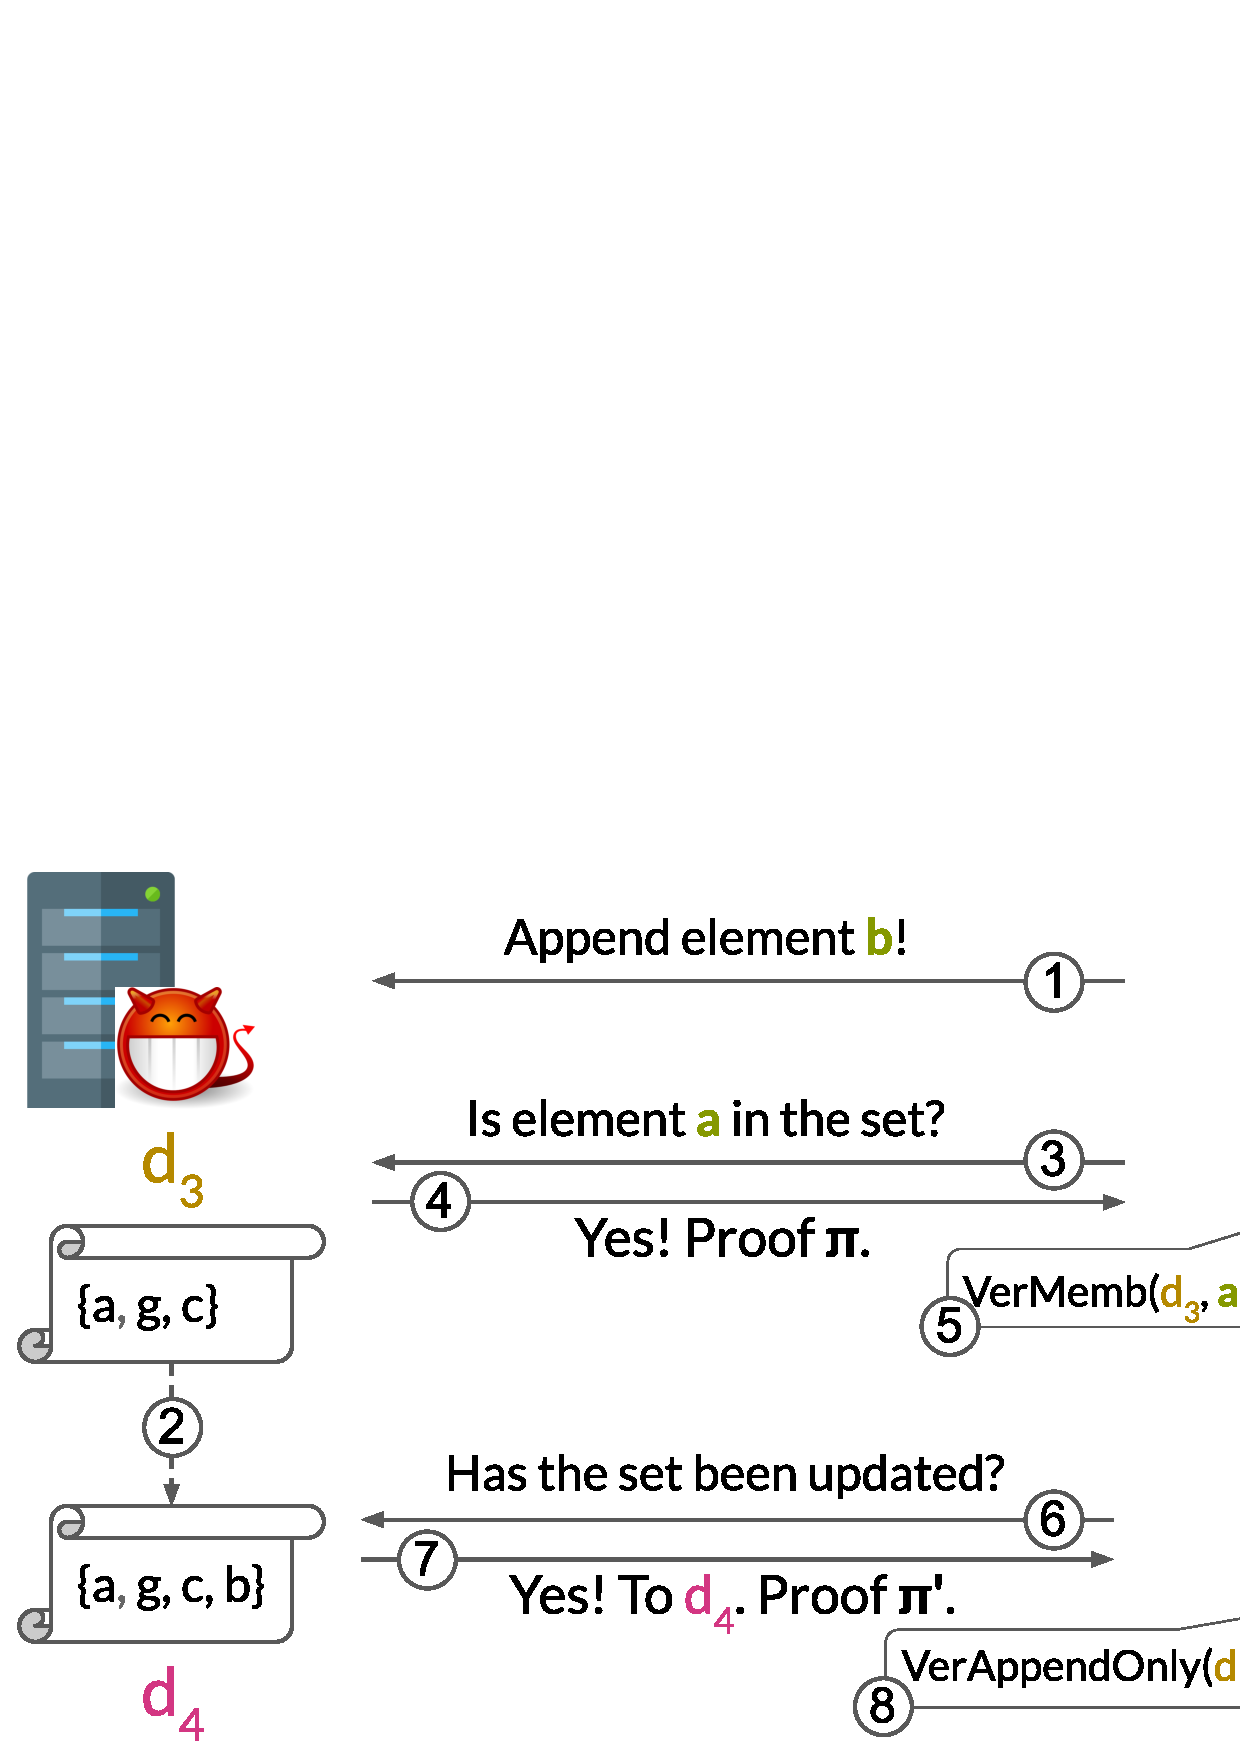
\includegraphics[width=.9\columnwidth]{figures-aad/model.pdf}
    %\vspace{-.5cm}
    \caption{
        Our model: a single malicious \textit{server} manages a \textit{set} and many \textit{clients} query the set.
        Clients will not necessarily have the digest of the latest set.
        The clients can (1) append a new element to the set, (2) query for an element and (3) ask for an updated digest of the set.
    }
    \label{f:model}
    %\vspace{-1.5em}
\end{figure}
}

\figModel

We begin by introducing a new primitive called an \textit{append-only authenticated set} (AAS).
An AAS is just a universal accumulator~\cite{LLX07} that supports subset witnesses and is fork-consistent.
We formalize the notion of an AAS in \cref{s:aas:defs} and instantiate it \textit{efficiently} from bilinear and RSA accumulators in \cref{s:aas:from-bilinear-acc} and in \cref{s:aas:from-rsa-acc}, respectively.
Then, in \cref{s:aad}, we slightly modify our AAS constructions to obtain \textit{append-only authenticated dictionaries} (AADs), which can be used to implement any transparency log~\cite{ELC16}.
Nonetheless, an AAS is useful in and of itself.
For example, it can be used for Revocation Transparency (RT)~\cite{Laurie15} to efficiently check the revocation status of certificates.

An AAS is a set of \textit{elements} managed by an \textit{untrusted server} and queried by \textit{clients}.
The server is the sole author of the AAS: it can append elements on its own and/or accept elements from clients.
% e.g., from History Tree paper: "Tamper-evident logs are fundamentally different: An untrusted logger is the sole author of the log and is responsible for both building and signing it.
% This is different from other models where elements might come from a \textit{trusted source} who signs them~\cite{two-party-ad,pads}.
Clients can check membership of elements in the set (see Steps 3-5 in \cref{f:model}).
Clients, also known as \textit{users}, are mutually-distrusting, potentially malicious, and do not have identities (i.e., no authorization or authentication).
Initially, the set starts out empty at \textit{version} zero, with new appends increasing its size and version by one.
Importantly, once an element has been appended to the set, it remains there forever: an adversary cannot remove nor change the element.
After each append, the server signs and publishes a new, small-sized \emph{digest} of the updated set (e.g., Step 2).

Clients periodically update their view of the set by requesting a new digest from the server (e.g., Step 6 and 7).
The new digest could be for an arbitrary version $j > i$, where $i$ is the previous version of the set (not just for $j = i+1$).
Importantly, clients always ensure the set remains \textit{append-only} by verifying an \textit{append-only proof} $\pi_{i,j}$ between the old and new digest (e.g., Step 8).
This way, clients can be certain the malicious server has not removed any elements from the set.
Clients will not necessarily have the latest digest of the set.
Finally, clients securely check if an element $k$ is in the set via a \emph{(non)membership proof} (e.g., Steps 3-5 in \cref{f:model}).

A malicious server can \emph{fork} clients' views~\cite{LKMS04}, preventing them from seeing each other's appends.
To deal with this, clients maintain a \textit{fork-consistent} view~\cite{LM07Beyond,LKMS04} of the set by checking append-only proofs.
As a consequence, if the server ever withholds an append from one client, that client's digest will forever diverge from other clients' digests.
To detect such \textit{forks}, clients can \textit{gossip}~\cite{CSP+15,STV+16,TD17,DPV+18} with one another about their digests.
This is crucial for security in transparency logs.

This model is the same as in history trees (HTs)~\cite{ht}, assuming only a gossip channel and no trusted third parties.
It also arises in encrypted web applications~\cite{mylar,verena,frientegrity}, Certificate Transparency (CT)~\cite{ct} and software transparency schemes~\cite{at,chainiac}.
Unlike the 2- and 3-party models~\cite{two-party-ad,pads,balloon}, there is no \textit{trusted source} that signs appends in this model.
A trusted source trivially solves the AAS/AAD problem as it can simply vouch for the data structure's append-only property with a digital signature.
Unfortunately, this kind of solution is useless for transparency logs~\cite{ct,Ryan2014,coniks}, which lack trusted parties.

        
        \section{Definitions}
        \label{s:aas:defs}
        \subsection{Server-side API}
The untrusted server implements:
\vspace{1em}

\api {\setup}$(1^\lambda, \upperbound) \rightarrow \pp, \vk$.
Randomized algorithm that returns public parameters $\pp$ used by the server and a \textit{verification key} $\vk$ used by clients.
Here, $\lambda$ is a security parameter and $\upperbound$ is an upper-bound on the number of elements $n$ in the set (i.e., $n \le \upperbound$).

\api {\append}$(\pp, \AS_i, d_i, k) \rightarrow \AS_{i+1}, d_{i+1}$.
Deterministic algorithm that appends a new element $k$ to the version $i$ set, creating a new version $i+1$ set.
Succeeds only if the set is not full (i.e., $i + 1 \le \upperbound$).
Returns the new authenticated set $\AS_{i+1}$ and its digest $d_{i+1}$.

\api $\provememb(\pp, \AS_i, k) \rightarrow b, \pi$.
Deterministic algorithm that proves (non)membership for element $k$.
When $k$ is in the set, generates a membership proof $\pi$ and sets $b=1$.
Otherwise, generates a non-membership proof $\pi$ and sets $b=0$.

\api {\proveappendonly}$(\pp, \AS_i, \AS_j) \rightarrow \pi_{i, j}$.
Deterministic algorithm that proves $\AS_i \subseteq \AS_j$.
In other words, generates an \textit{append-only proof} $\pi_{i, j}$ that all elements in $\AS_i$ are also present in $\AS_j$.
Importantly, a malicious server who removed elements from $\AS_j$ that were present in $\AS_i$ cannot construct a valid append-only proof.

\subsection{Client-side API}
Clients implement:
\vspace{1em}

\api {\vermemb}$(\vk, d_i, k, b, \pi) \rightarrow \{T, F\}$.
Deterministic algorithm that verifies proofs returned by $\provememb(\cdot)$ against the digest $d_i$.
When $b=1$, verifies $k$ is in the set via the membership proof $\pi$.
When $b=0$, verifies $k$ is \textit{not} in the set via the non-membership proof $\pi$.
(We formalize security in \cref{s:aas:correctness-and-security}.)

\api {\verappendonly}$(\vk, d_i, i, d_j, j, \pi_{i,j}) \rightarrow \{T, F\}$.
Deterministic algorithm that ensures a set remains append-only.
Verifies that $\pi_{i,j}$ correctly proves that the set with digest $d_i$ is a subset of the set with digest $d_j$.
Also, verifies that $d_i$ and $d_j$ are digests of sets at version $i$ and $j$, respectively, enforcing fork consistency.

\paragraph{Using the API.}
To use an AAS scheme, first, public parameters need to be computed using a call to $\setup(\cdot)$.
If the AAS scheme is trapdoored, a trusted party runs $\setup(\cdot)$ and forgets the trapdoor. 
(This can be securely implemented via a multi-party computation protocol~\cite{GMW87}.)
Once computed, the parameters can be reused by different servers for different append-only sets.
$\setup(\cdot)$ also returns a \textit{public} verification key $\vk$ to all clients.

Then, the server broadcasts the initial digest $d_0$ of the empty set $\AS_0$ to its many clients.
Clients can concurrently start appending elements using $\append(\cdot)$ calls.
If the server is honest, it serializes $\append(\cdot)$ calls.
Eventually, the server returns a new digest $d_i$ to clients along with an append-only proof $\pi_{0,i}$ computed using $\proveappendonly(\cdot)$.
Some clients might be offline but eventually they will receive either $d_i$ or a newer $d_j, j > i$.
Importantly, whenever clients transition from version $i$ to $j$, they check an append-only proof $\pi_{i,j}$ using $\verappendonly(\vk, d_i, i, d_j, j, \pi_{i,j})$.

Clients can look up elements in the set.
The server proves (non)membership of an element using $\provememb(\cdot)$.
A client verifies the proof using $\vermemb(\cdot)$ against their digest.
As more elements are added by clients, the server continues to publish a new digest $d_j$ and can prove it is a superset of any previous digest $d_i$ using $\proveappendonly(\cdot)$.

\subsection{Correctness and Security}
\label{s:aas:correctness-and-security}
We first introduce some helpful notation for our correctness definitions.
Consider an ordered sequence of $n$ appends $(k_i)_{i\in [n]}$.
% --- begin multiline ---
Let 
$\AS',d' \leftarrow \multiappend(\pp, \AS, d, (k_i)_{i\in [n]})$ 
denote a sequence of $\append(\cdot)$ calls arbitrarily interleaved with other $\provememb(\cdot)$ and $\proveappendonly(\cdot)$ calls such that 
$\AS',d'$ $\leftarrow$ $\append(\pp,\AS_{n-1}$, $d_{n-1}, k_{n})$,
$\AS_{n-1}, d_{n-1}$ $\leftarrow$ $\append(\pp,\AS_{n-2}, d_{n-2}, k_{n-1})$,
$\dots$,
$\AS_{1}, d_1$ $\leftarrow$ $\append(\pp,\AS, d, k_{1})$.
% --- end of multiline ---
Finally, let $\AS_0$ denote an empty AAS with empty digest $d_0$.

\begin{definition}[Append-only Authenticated Set]
    \label{def:secure-aas-definition}
    (\setup, \append, \provememb, \proveappendonly, \vermemb, \verappendonly) is a secure append-only authenticated set (AAS) if
    $\forall$ upper-bounds $\upperbound=\poly(\lambda)$ it satisfies the following properties:
\end{definition}

\begin{definition}[AAS Membership Correctness]
\label{def:aas:membership-correctness}
$\forall n \le \upperbound$, $\forall$ ordered sequences of appends $(k_i)_{i\in[n]}$, for all elements $k$, where $b=1$ if $k\in (k_i)_{i\in[n]}$ and $b=0$ otherwise,
\begin{align*}
\Pr \left[ \begin{array}{c}
(\pp,\vk) \leftarrow \setup(1^\lambda, \upperbound),\\
(\AS, d) \leftarrow \multiappend(\pp, \AS_0, d_0, (k_i)_{i\in[n]}),\\
(b',\pi) \leftarrow \provememb(\pp,\AS, k): \\
{{b=b'}\wedge{\vermemb(\vk, d, k, b, \pi) = T}}
\end{array} \right]
\ge 1 - \negl(\lambda)
\end{align*}
\end{definition}

\noindent \textit{Observation:}
Note that this definition compares the returned bit $b'$ with the ``ground truth'' in $(k_i)_{i\in[n]}$ and thus provides membership correctness.
Also, it handles non-membership correctness since $b'$ can be zero.
Finally, the definition handles all possible orders of appending elements.


\begin{definition}[AAS Membership Security]
\label{def:aas:membership-security}
$\forall$ adversaries \Adv running in time $\poly(\lambda)$,
\begin{align*}
\Pr \left[ \begin{array}{c}
(\pp,\vk) \leftarrow \setup(1^\lambda, \upperbound), \\
(d, k,\pi,\pi') \leftarrow \Adv(1^\lambda, \pp, \vk)
: \\
{\vermemb(\vk,d, k,0,\pi ,) = T} \wedge {} \\
{\vermemb(\vk,d, k,1,\pi',) = T}
\end{array} \right] \le \negl(\lambda)
\end{align*}
\end{definition}

\noindent \textit{Observation (1):}
This definition captures the lack of any ``ground truth'' about what was inserted in the set, since there is no trusted source in our model.
Nonetheless, given a fixed digest $d$, our definition prevents \textit{all} equivocation attacks about the membership of an element in the set.

\noindent \textit{Observation (2):}
These definitions imply \textit{collision-resistance}: i.e., different sets cannot have the same digest.
To see this, suppose you have two different sets with the same digest.
Since the sets differ, there exists an element $x$ that is in the first set but not the second set (without loss of generality).
Then, membership correctness guarantees you can create a valid membership proof for $x$ w.r.t. the first set and a non-membership proof for $x$ w.r.t. the second set.
As a result, we will have both a membership and a non-membership proof for $x$ that verifies w.r.t. the same digest.
This breaks membership security and leads to a contradiction.


\begin{definition}[AAS Append-only Correctness]
\label{def:aas:appendonly-correctness}
$\forall n \le \upperbound$, $\forall m < n,\forall$ sequences of appends $(k_i)_{i\in[n]}$ where $n\ge2$,
\begin{align*}
\Pr \left[ \begin{array}{c}
(\pp,\vk) \leftarrow \setup(1^\lambda, \upperbound) \\
(\AS_m, d_m) \leftarrow \multiappend(\pp,\AS_0,d_0,(k_i)_{i\in[m]}),\\
(\AS_n, d_n) \leftarrow \multiappend(\pp,\AS_m,d_m,(k_i)_{i\in[m+1,n]}),  \\
\pi \leftarrow \proveappendonly(\pp,\AS_m, \AS_n):\\
{\verappendonly(\vk, d_m, m, d_n, n, \pi) = T}
\end{array} \right] \ge 1 - \negl(\lambda)
\end{align*}
\end{definition}

\begin{definition}[AAS Append-only Security]
\label{def:aas:appendonly-security}
$\forall$ adversaries \Adv running in time $\poly(\lambda)$,
\begin{align*}
\Pr \left[ \begin{array}{c}
(\pp,\vk) \leftarrow \setup(1^\lambda, \upperbound)\\
(d_i,d_j,i < j,\pi_a, k,\pi,\pi') \leftarrow \Adv(1^\lambda, \pp, \vk)
: \\
{\verappendonly(\vk, d_i, i, d_j, j, \pi_a) = T} \wedge {}\\
{\vermemb(\vk, d_i, k, 1, \pi )  = T} \wedge {}\\
{\vermemb(\vk, d_j, k, 0, \pi') = T}
\end{array} \right] \le \negl(\lambda)
\end{align*}
\end{definition}

\noindent \textit{Observation:}
This definition ensures that elements can only be added to an AAS.

\begin{definition}[Fork Consistency]
\label{def:aas:fork-consistency}
$\forall$ adversaries \Adv running in time $\poly(\lambda)$,
\begin{align*}
\Pr \left[ \begin{array}{c}
(\pp,\vk) \leftarrow \setup(1^\lambda, \upperbound)\\
(d_i\ne d_i',d_j,i<j,\pi_i,\pi_i') \leftarrow \Adv(1^\lambda, \pp, \vk)
: \\
{\verappendonly(\vk, d_i , i, d_j, j, \pi_i) = T} \wedge {}\\
{\verappendonly(\vk, d_i', i, d_j, j, \pi_i') = T}\\
\end{array} \right] \le \negl(\lambda)
\end{align*}
\end{definition}

\noindent \textit{Observation:}
This is our own version of fork consistency that captures what is known in the literature about fork consistency~\cite{ht,LM07Beyond}.
Specifically, it allows a server to fork the set at version $i$ by presenting two different digests $d_i$ and $d_i'$ and prevents the server from forging append-only proofs that ``join'' the two forks into some common digest $d_j$ at a later version $j$.

        
        \section{AAS from Bilinear Accumulators}
        \label{s:aas:from-bilinear-acc}
        \newcommand{\communionTreeFig}{
%\begin{landscape}
\begin{figure*}[t]
{
    %\tiny
    %\scriptsize
    %\footnotesize
    %\small
    %\normalsize
    \begin{center}
    \begin{forest}
    %for tree={
    %    fit=band,% spaces the tree out a little to avoid collisions
    %    fit=tight,% spaces the tree out less
    %    fit=rectangle,
    %    inner sep=4,
    %}
    [{$g^{(s-e_1)(s-e_2)(s-e_3)(s-e_4)}$}
        [{$g^{(s-e_1)(s-e_2)}$}
            [{$g^{(s-e_1)}$}
                %[, no edge, tier=odd ]
            ]
            [{$g^{(s-e_2)}$}
                %[, no edge, tier=odd ]
            ]
        ]
        [{$g^{(s-e_3)(s-e_4)}$} 
            [{$g^{(s-e_3)}$}
                %[, no edge, tier=odd ]
            ]
            [{$g^{(s-e_4)}$}
                %[, no edge, tier=odd ]
            ]
        ]
    ]
    \end{forest}
    \end{center}
} % end of \tiny\scriptisize\whatever
\caption{A \communionTree (CT) over the set $\{e_1, e_2, e_3, e_4\}$.
The leaves store bilinear accumulators over the individual elements.
Every non-leaf node stores a bilinear accumulator over all elements from its subtree's leaves.}
\label{f:comm-tree}
\end{figure*}
%\end{landscape}
} % end of \newcommand

\newcommand{\accumulatedTreeFig}{
\begin{figure}[t]
    \centering
    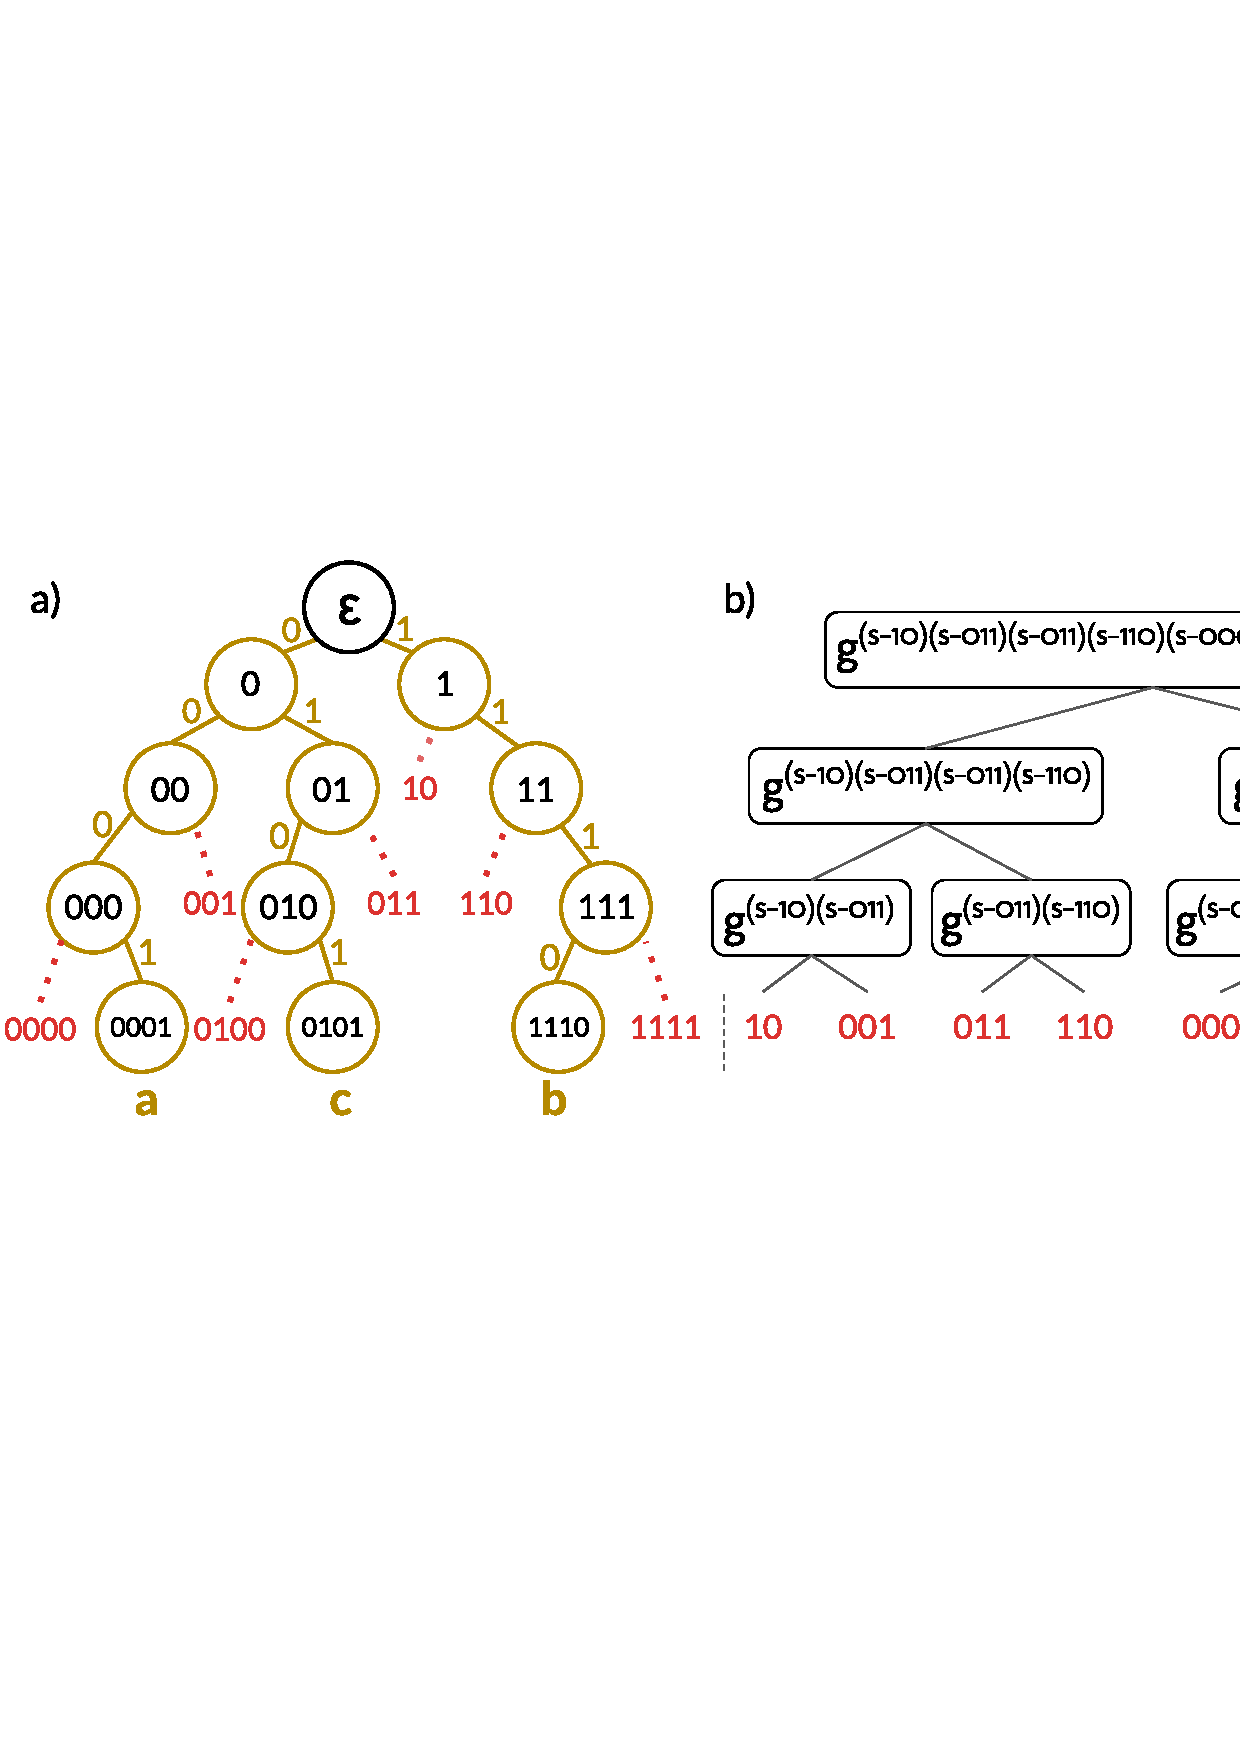
\includegraphics[width=.95\columnwidth]{figures-aad/AT.pdf}
    \vspace{-15em}
    \caption{
        On the left side, we depict a trie over set $S = \{a,b,c\}$.
        Each element is mapped to a unique path of length $4$ in the trie.
        (Here, $\lambda=2$.)
        Nodes that are not in the trie but are at its \textit{frontier} are depicted in \myred{\textbf{red}}.
        On the right side, we depict a \textit{\frontierCommunionTree} (FCT) corresponding to the set $S$.
        To prove that an element is not in $S$, we prove one of its prefixes is in the FCT.
        \label{f:accumulated-tree}}
    %\vspace{-2.5em}
\end{figure}
}

\newcommand{\forestFig}{
\begin{figure}[t]
    \centering
    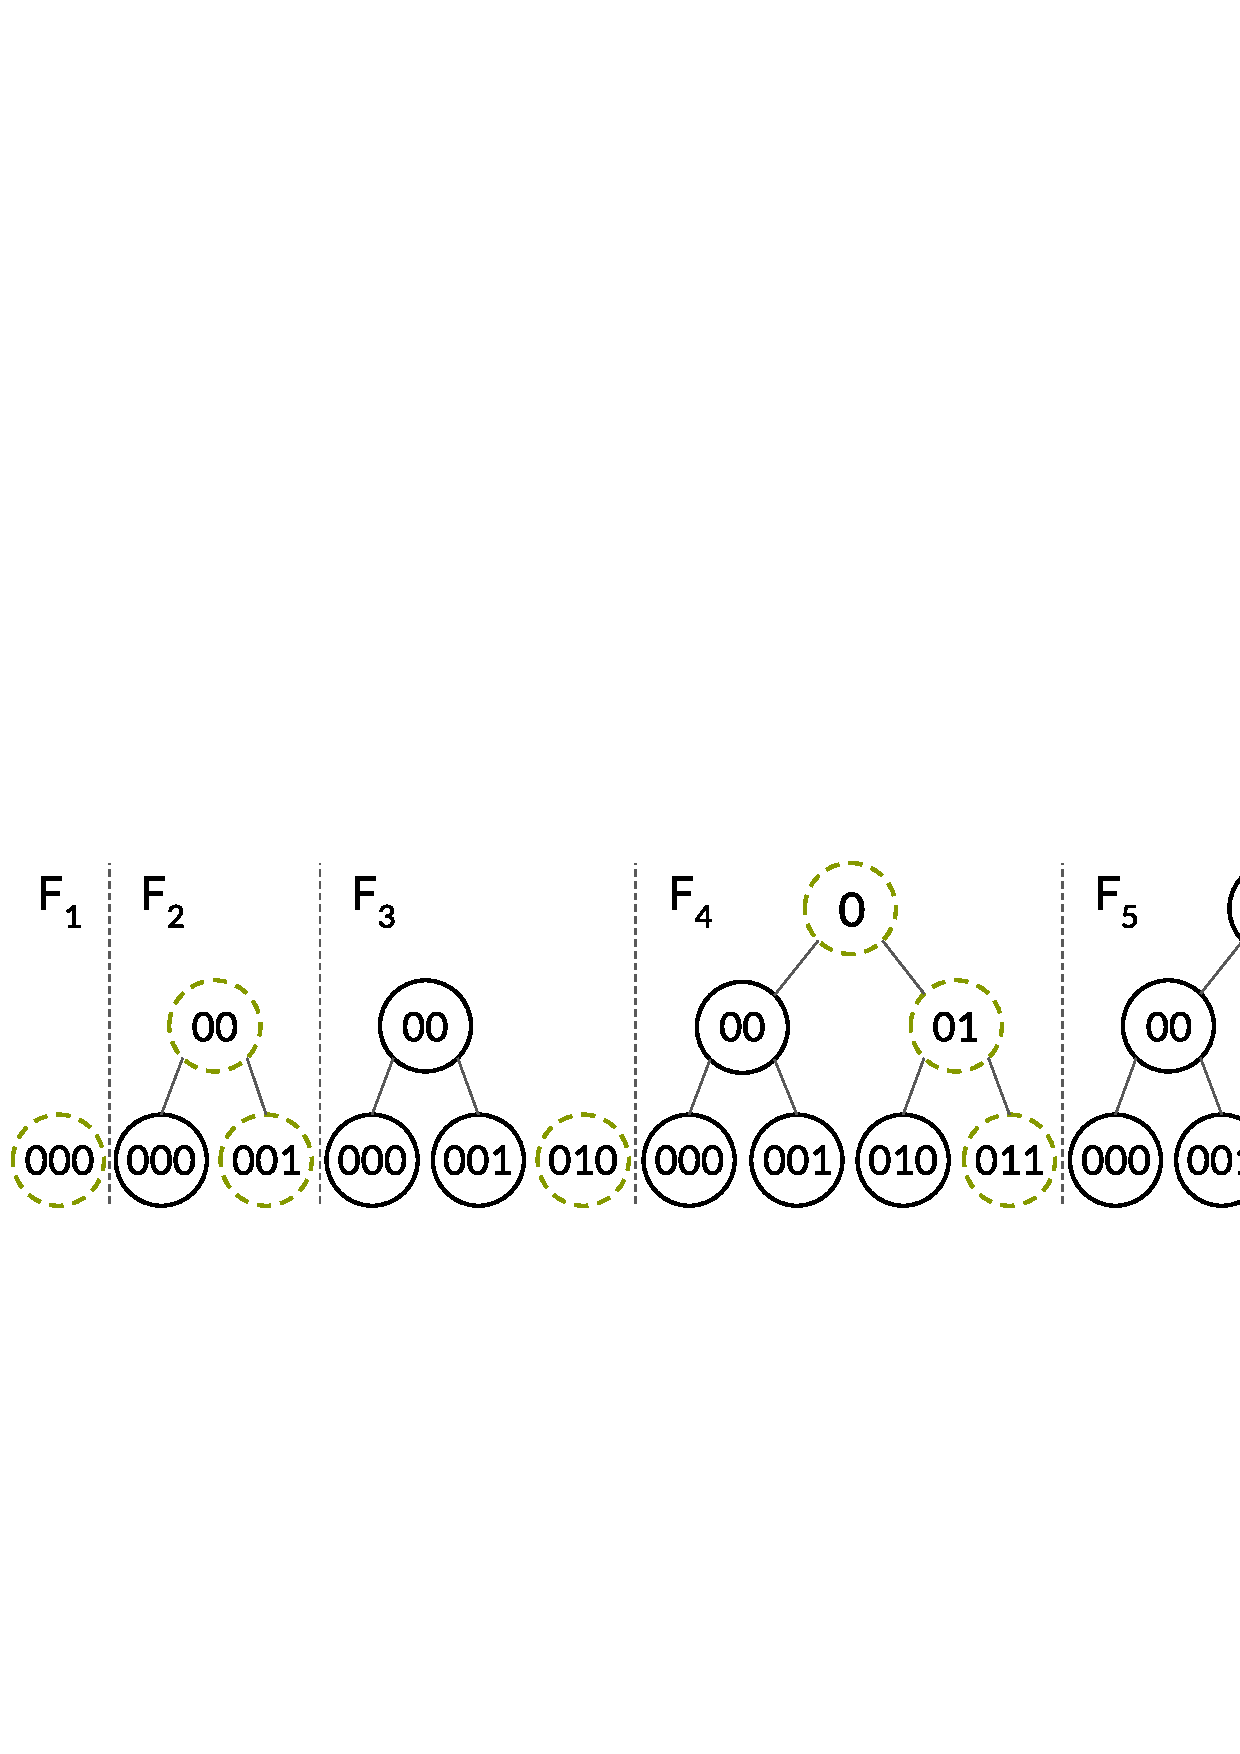
\includegraphics[width=.95\columnwidth]{figures-aad/forest.pdf}
    \vspace{-13em}
    \caption{
        A forest starting empty and going through a sequence of five appends.
        A forest only has trees of exact size $2^j$ for distinct $j$'s.
        A forest of $n$ leaves has \textit{at most} $\log{n}$ trees. 
    }
    \label{f:forest}
\end{figure}
}

\newcommand{\amortizedAasFig}{
\begin{figure}[t]
    \centering
    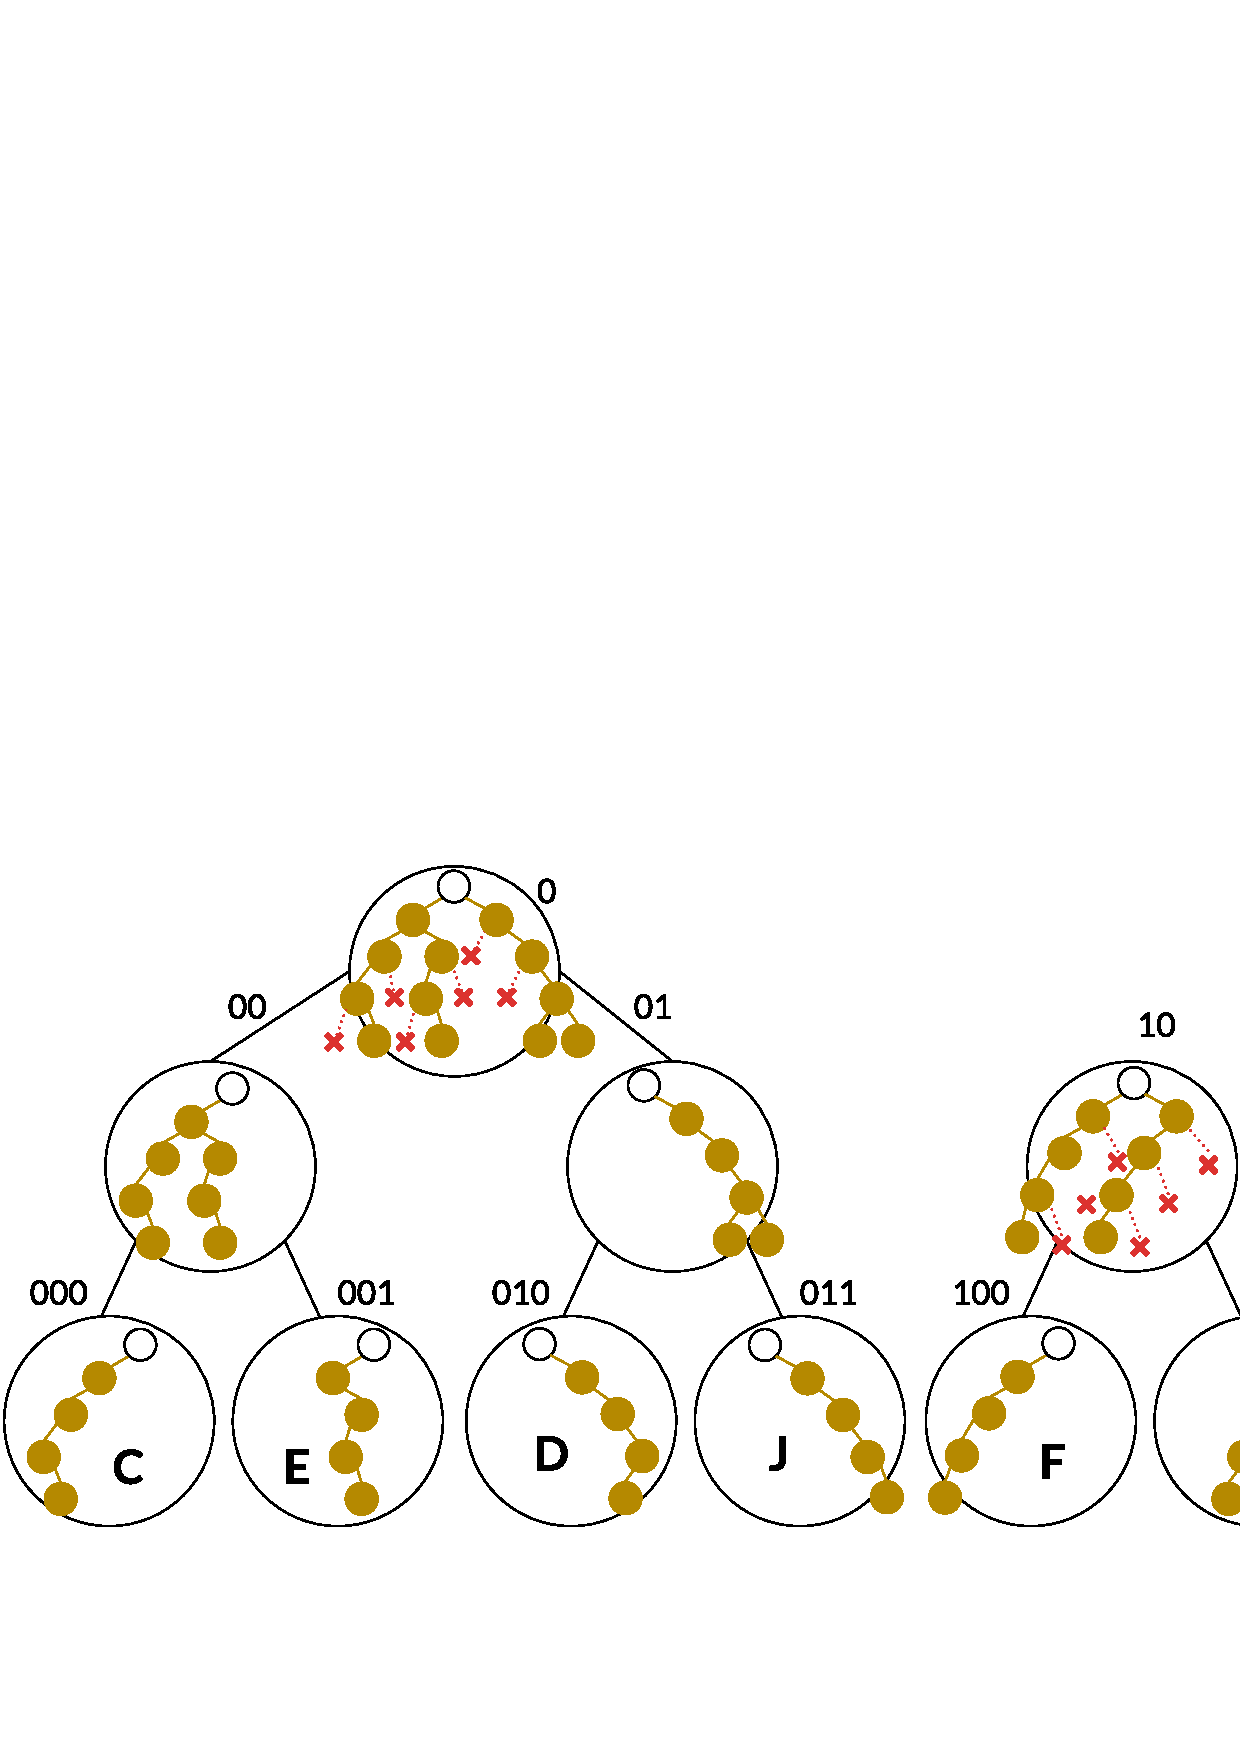
\includegraphics[width=.90\columnwidth]{figures-aad/accaas.pdf}
    \vspace{-1.7cm}
    \caption{
        A dynamic AAS with $\lambda=2$ for set $\{B,C,D,E,F,H,J\}$.
        Our AAS is a forest of PCTs with corresponding FCTs.
        Each node stores a prefix accumulator (and subset witness), depicted as a trie, in \myyellow{yellow}.
        Root nodes store an FCT, depicted as the missing \myred{red} nodes.
    }
    \label{f:accaas}
\end{figure}
}

This section presents our bilinear accumulator-based AAS construction.
We give a more formal, algorithmic description of this construction in \cref{s:aas:from-bilinear-acc:algorithms}.
We prove this construction secure under the $q$-SBDH and $q$-PKE assumptions in \cref{s:aas:from-bilinear-acc:proofs:membership-security}.
Finally, in \cref{s:aas:from-rsa-acc}, we present our RSA accumulator-based AAS.

As mentioned in \cref{s:intro:overview-techniques}, a bilinear accumulator over $n$ elements is already an AAS, but with two caveats: it is not fork-consistent (see \cref{def:aas:fork-consistency}) and it is computationally inefficient.
Specifically, proving (non)membership in a bilinear accumulator requires an $O(n)$ time polynomial division.
As a consequence, precomputing all $n$ membership proofs (naively) takes $O(n^2)$ time, which is prohibitive for most use cases.
Even worse, for non-membership, one must precompute proofs for all possible missing elements, of which there are exponentially many (in the security parameter $\lambda$).
Therefore, we need new techniques to achieve our desired polylogarithmic time complexity for computing both types of proofs in our AAS.

\subsection{Precomputing Membership with \communionTrees (CTs)}
\label{s:aas:from-bilinear-acc:ct}

\communionTreeFig

Our first technique is to deploy the bilinear accumulator in a tree structure, as follows.
We start with the elements $e_i$ as leaves of a binary tree (see \cref{f:comm-tree}).
Specifically, each leaf will store an accumulator over the singleton set $\{e_i\}$.
Every internal node in the tree will then store an accumulator over the union of the sets corresponding to its two children.
For example, the parent node of the two leaves corresponding to $\{e_i\}$ and $\{e_{i+1}\}$ stores the accumulator of the set $\{e_i,e_{i+1}\}$.
In this way, the root is the accumulator over the full set $S = \{e_1,\dots,e_n\}$ (see \cref{f:comm-tree}).

We stress that all accumulators in the tree use the same public parameters.
The time to compute all the accumulators in the tree is $T(n) = 2T(n/2) + O(n\log{n}) = O(n\log^2{n})$ where $O(n\log{n})$ is the time to multiply the characteristic polynomials of two sets of size $n$ in the tree.
We call the resulting structure a \textit{Comm(itment) Union Tree} or \emph{\communionTree} (CT) over set $S$, since every node in the tree is a commitment to the union of that node's childrens' committed sets.
A similar technique of ``unioning-and-then-accumulating'' sets in a tree first appeared in~\cite{CG10}.

A membership proof for element $e_i$ will leverage the fact that sets along the path from $e_i$'s leaf to the root of the \communionTree are subsets of each other.
The proof will consist of a sequence of \textit{subset witnesses} that validate this (computed as explained in \cref{s:prelim:bilinear-acc}).
Specifically, the proof contains the accumulators along the path from $e_i$'s leaf to the root, as well as the accumulators of all sibling nodes along this path (see \cref{f:comm-tree}).
The client verifies all these subset witnesses, starting from the singleton set $\{e_i\}$ in the leaf.
This convinces  him that $e_i$ is contained in the parent's accumulated set, which in turn is contained in its parent's accumulated set and so on, until the root.

Our CT approach gives us membership proofs of logarithmic size and thus logarithmic verification time.
Importantly, computing a \communionTree in $O(n\log^2{n})$ time implicitly computes all membership proofs ``for free''!
In contrast, building a standard billinear accumulator over $S$ would yield constant-size proofs but in $O(n^2)$ time for all $n$ proofs.
Unfortunately, CTs cannot (yet) precompute non-membership proofs, which we address next.

\accumulatedTreeFig

\subsection{Precomputing Non-membership by Accumulating Prefixes}
The \communionTree (CT) technique can efficiently precompute all $n$ membership proofs.
For non-membership though, we have to somehow precompute proofs for an exponential number of elements in the security parameter $\lambda$.
(Recall that an element is just a number $e\in \Fp$ where $p\approx 2^{2\lambda}$.)
For this, we build upon old ideas in computer science.

Specifically, we represent the set of elements as binary strings of length $2\lambda$ bits.
Thus, the set can be viewed as a \textit{trie} (see \cref{f:accumulated-tree}a).
As a consequence, when an element is not in the set, one of the prefixes of its binary string will not be in the trie.
Our key observation is that precomputing all proofs for such missing prefixes in effect precomputes all non-membership proofs.
This ``missing prefixes'' technique is also used in Micali et al.'s zero-knowledge sets~\cite{zks}.
We introduce it gradually below.

\subsubsection{\prefixCommunionTrees (PCTs)}
\label{s:aas:from-bilinear-acc:pct}
To efficiently precompute non-membership proofs, we slightly modify our CT construction into a \prefixCommunionTree (PCT).
As before, a parent's set is the union of its children's sets, but the key difference is that leaves will no longer store an individual element $e_i$ but will store all prefixes $\prefixes(e_i)$ of its binary representation.
We assume this representation is $2\lambda$ bits (or is made so using a CRHF) and can be mapped to an element in $\Fp$ (which is also of size $\approx 2\lambda$ bits) and thus can be accumulated.

For example, a leaf that previously stored element $e_1$ with binary representation $0001$, will now store the set $\prefixes(e_1) = \{\varepsilon,0,00,000,0001\}$ (i.e., all the prefixes of the binary representation of $e_1$, including the empty string $\varepsilon$).
Also, for any set $S = \{e_1,\dots,e_n\}$, we define its \emph{prefix set} as $\prefixes(S) = \prefixes(e_1) \cup \dots \cup \prefixes(e_n)$.
For example, let $S =\{a=0001,b=0101,c=1110\}$.
Then, the root of $S$'s \prefixCommunionTree will contain a \textit{prefix accumulator} over $\prefixes(S) = \prefixes(a) \cup \prefixes(b) \cup \prefixes(c) = \{\varepsilon,0,1,00,01,11,000,010,111,0001,0101,1110\}$.
We refer to accumulators in PCT nodes as prefix accumulators since they accumulate prefixes of elements, rather than elements themselves.

The time to build a PCT for $S$ is $O(\lambda n\log^2{n})$ since there are $O(\lambda n)$ prefixes across all leaves.
Note that membership proofs in a PCT are the same as in CTs, with a minor change.
The internal nodes of the tree still store accumulators over the union of their children.
However, the children now have common prefixes, which will only appear once in the parent.
For example, two children sets have the empty string $\varepsilon$ while their parent set only has $\varepsilon$ once (because of the union).
As a result, it is no longer the case that multiplying the characteristic polynomials of the children gives us the parent's polynomial.
Therefore, we can no longer rely on the siblings as subset witnesses: we have to explicitly compute subset witnesses for each child w.r.t. its parent.
We stress that this does not affect the asymptotic time complexity of computing the PCT.
As before, the client starts the proof verification from the leaf, which now stores a prefix set $\prefixes(e_i)$ rather than a singleton set $\{e_i\}$.

\subsubsection{\frontierCommunionTree (FCTs)}
\label{s:aas:from-bilinear-acc:fct}
But how does a PCT help with precomputing non-membership proofs for any element $e'\notin S$?
First, note that to prove $e'\notin S$ it suffices to show that \textit{any one prefix $\rho$ of $e'$ is not contained in $\prefixes(S)$}.
Second, note that there might exist other elements $e''$ who share $\rho$ as a prefix.
As a result, the non-membership proof for $e'$ could be ``reused'' as a non-membership proof for $e''$.

This is best illustrated in \cref{f:accumulated-tree}a using our previous example where $S =\{a,b,c\}$.
Consider elements $d= \underline{011}1$ and $f = \underline{011}0$ that are not in $S$.
To prove non-membership for either element, it suffices to prove the same statement: $\underline{011}\notin \prefixes(S)$.
Thus, if we can identify all such shared prefixes, we can use them to prove the non-membership of (exponentially) many elements.

First, note that prefix accumulator of a set $S$ is just a \textit{trie}, as depicted in \cref{f:accumulated-tree}a.
The key idea is to keep track of the prefixes at the ``frontier'' of the trie, depicted in \myred{\textbf{red}} in \cref{f:accumulated-tree}a.
Informally, these \textit{frontier prefixes} are prefixes that are \textit{not} in the trie but have a \textit{parent} in the trie (e.g., 011 is not in the trie but its parent 01 is).
We immediately notice that to prove non-membership of any element, it suffices to prove non-membership of one of these frontier prefixes!
In other words, elements that are not in $S$ will have one of these as a prefix.
We can formally define the \textit{frontier} of $S$ as:
\begin{align*}
    F(S) &= \{\rho \in \{0,1\}^{\le 2\lambda}: {\rho\not \in \prefixes(S)} \wedge {\parent(\rho) \in \prefixes(S)}\}\text{,}
\end{align*}
where $\parent(\rho)$ is $\rho$ without its last bit (e.g., $\parent(011) = 01$).
Note that the size of $F(S)$ is $O(\lambda n)$, proportionate to $\prefixes(S)$.

Most importantly, from the way $\prefixes(S)$ and $F(S)$ are defined, for any element $e'$, it holds that $e'\not\in S$ if, and only if, some prefix of $e'$ is in $F(S)$. 
Therefore, proving non-membership of $e'$ boils down to proving two statements: (i) some prefix of $e'$ belongs to $F(S)$, and (ii) $\prefixes(S) \cap F(S) = \varnothing$.
We stress that the latter is necessary as a malicious server may try to craft $F(S)$ in a false way (e.g., by adding some prefixes both in $\prefixes(S)$ and in $F(S)$).

To prove (i), we build a \communionTree over $F(S)$ which gives us precomputed membership proofs for all $\rho \in F(S)$ (see \cref{f:accumulated-tree}b).
We refer to this tree as the \emph{\frontierCommunionTree (FCT)} for set $S$, to the proofs as \textit{frontier proofs}, and to the accumulators in the tree as \textit{frontier accumulators}.
To prove (ii), we compute a \emph{disjointness witness} between sets $\prefixes(S)$ and $F(S)$, as described in \cref{s:prelim:polycommit} (i.e., between the root prefix accumulator and the root frontier accumulator).
The time to build a FCT for $S$ is $O(\lambda n\log^2{n})$ since $F(S)$ has $O(\lambda n)$ elements.
The disjointness witness can also be computed in $O(\lambda n\log^2{n})$ time.

\subsection{From Static to Dynamic AAS}

Combining all the above techniques, we obtain a \textit{static} AAS that does \textit{not yet} support updates efficiently (nor append-only proofs).
This construction consists of: (a) a PCT for $S$, (b) a FCT for $S$, and (c) a disjointness witness for $\prefixes(S)$ and $F(S)$ (i.e., between the root prefix and frontier accumulators).
The height of the PCT is $O(\log n)$ and the height of the FCT is $O(\log{(\lambda n)})$ so the size and verification time of a (non)membership proof is $O(\log{n})$.
The digest is just the root prefix accumulator of the PCT. 

\subsubsection{Appending Efficiently in Polylogarithmic Time}
Our AAS should \textit{efficiently} support appending new elements to $S$. 
The main challenge here is that updating the PCT and FCT as well as the disjointness witness after each update is very expensive (i.e., at least linear time in their size).
To address this we use a classic ``amortization'' trick from Overmars~\cite{overmars} also used in~\cite{distributed-acc}. 
Specifically, our AAS will consist not of one PCT for the entire set $S$, but of a \textit{forest} of PCTs and their corresponding FCTs.
The idea is to maintain a partitioning of $S$ with $1 + \floor{\log{|S|}}$ disjoint subsets, each of a distinct size $2^i$.

\forestFig

Initially, we start with no elements in the AAS.
When the first element $e_1$ is appended, we build its PCT over the set $\{e_1\}$, its FCT and a disjointness witness.
Together, these make up the \textit{CT-pair} of a set $S$ (in this case, $S=\{e_1\}$).
When the second element $e_2$ is appended, we ``merge'': we build a CT-pair over $\{e_1, e_2\}$.
We define the \textit{size of a CT pair} as the size of its set $S$ (in this case, the size is 2 since $S=\{e_1,e_2\}$).
The rule is we always merge equal-sized CT-pairs.
When $e_3$ is appended, we cannot merge it because there's no other CT-pair of size 1.
Instead, we create a CT-pair over $\{e_3\}$.

In general, after $2^\ell - 1$ appends, we end up with $\ell$ separate CT-pairs corresponding to sets of elements $S_1,\dots,S_\ell$.
The final set is $S=\bigcup_{j=1}^{\ell} S_j$ where $|S_j| = 2^j$.
The evolution of such a forest is depicted in \cref{f:forest} and the final data structure can be seen in \cref{f:accaas}.
In \cref{s:aas:from-bilinear-acc:asymptotics}, we show this approach gives us an $O(\lambda n\log^3 {n})$  \textit{amortized} append time.
Fortunately, generic \textit{de-amortization} techniques~\cite{overmars,overmars-van-leeuwen} can be used to obtain an $O(\lambda n\log^3 {n})$ \textit{worst-case} append time.

\amortizedAasFig

The downside of our amortized approach is that proving non-membership becomes slightly more expensive than in the static AAS data structure from above.
Specifically, now the server needs to prove non-membership in each CT-pair separately, requiring an $O(\log{n})$ frontier proof in each of the $O(\log{n})$ FCTs.
This increases the non-membership proof size to $O(\log^2 n)$.
On a good note, membership proofs remain unaffected: the server just sends a path to a leaf in \textit{one} of the PCTs where the element is found.
Finally, the AAS digest is set to the root prefix accumulators of all PCTs and has size $O(\log{n})$.
We analyze the complexity of our AAS in \cref{s:aas:from-bilinear-acc:asymptotics}.

\subsubsection{Logarithmic-sized Append-only Proofs}
Our append-only proofs are similar to the ones in history trees~\cite{ht}.
% Recall that when we merge the PCTs for $S_1, S_2$ and build a new PCT, (i) we compute its new root as the accumulator of $\prefixes(S_1) \cup \prefixes(S_2)$, (ii) we set the two old roots as the new root's children and (iii) we compute subset witnesses between the old roots and the new root.
% Thus, the old roots become children nodes in the new PCT.
% In fact, because every append to the AAS triggers a sequence of merges, we can generalize the above statement: after a sequence of appends, \textit{some} of the old roots in the old AAS will become descendants of a new root in the new AAS.
% The remaining old roots, if any, will remain as (new) roots in the new forest (e.g., root 0 from $F_4$ to $F_5$ in \cref{f:forest}).
% Our append-only proof leverages the above invariant.
An append-only proof must relate the root prefix accumulator(s) in the old AAS to the root prefix accumulator(s) in the new AAS.
We'll refer to these as ``old roots'' and ``new roots'', respectively.
Specifically, it must show that every old root either (i) became a new root or (ii) has a path to a new root with valid accumulator subset witnesses at every level.
Such a path is verified by checking the subset witnesses between every child and its parent, exactly as in a membership proof.
At the same time, note that there might be new roots that are neither old roots nor have paths to old roots (e.g., root 111 in $F_5$ from \cref{f:forest}).
The proof simply ignores such roots since they securely add new elements to the set.
To summarize, the append-only proof guarantees that each old root (1) has a valid subset path to a new root or (2) became a new root.

\paragraph{Ensuring Fork Consistency.}
For gossip protocols to work~\cite{CSP+15,DPV+18}, our AAS must be fork-consistent.
Interestingly, append-only proofs do not imply fork consistency.
For example, consider a server who computes an AAS for set $\{e_1\}$ and another one for the set $\{e_2\}$. 
The server gives the first set's digest to user $A$ and the second digest to user $B$.
Afterwards, he appends $e_2$ to the first set and $e_1$ to the second one, which ``joins'' the two sets into a common set $\{e_1,e_2\}$.
The append-only property was not violated (as the two users can deduce independently) but fork consistency has been: the two users had diverging views that were subsequently merged.

To avoid this, we will ``Merkle-ize'' each PCT using a CRHF $\Hb$ in the standard manner (i.e., a node hashes its prefix accumulator and its two children's hashes).
Our AAS digest is now set to the Merkle roots of all PCTs, which implicitly commit to all root prefix accumulators in the PCTs.
As a result, after merging PCTs for elements $e_1$ and $e_2$, the Merkle root of the merged PCT will differ based on how appends were ordered: $(e_1,e_2)$, or $(e_2,e_1)$.
Thus, violating fork consistency becomes as hard as finding a collision in $\Hb$.
(We prove this in \cref{s:aas:from-bilinear-acc:proofs:fork-consistency}.)

\subsection{Asymptotic Analysis}
\label{s:aas:from-bilinear-acc:asymptotics}

Suppose we have a \textit{worst-case} AAS with $n$ = $2^i - 1$ elements.

\paragraph{Append Time.}
First, let us analyze the time to merge two size-$n$ CT-pairs for two sets $S_1$ and $S_2$ into a size-$2n$ CT-pair for their union $S=S_1 \cup S_2$.
To compute $S$'s PCT, we need to (i) compute its prefix accumulator, (ii) set its children to the ``old'' prefix accumulators of $S_1$ and $S_2$ and (iii) compute subset witnesses for $S_1 \subset S$ and for $S_2\subset S$.
Since $|S_1|=|S_2|=n$, operations (i), (ii) and (iii) take $O(\lambda n \log^2{n})$ time.
Finally, we can compute $S$'s FCT from scratch in $O(\lambda n\log^2 n)$ time.

Now, consider the time $T(n)$ to create an AAS over a set $S$ with $n = 2^\ell$ elements (without loss of generality).
Then, $T(n)$ can be broken into:
\begin{itemize}
    \item The time to create a CT-pair over the children of $S$ of size $n/2$ (i.e., $2T(n/2)$).
    \item The time to merge these two CT-pairs, including computing subset witnesses (discussed above)
    \item The time to compute the FCT of $S$ (discussed above).
\end{itemize}
More formally, $T(n) = 2T(n/2) + O(\lambda n\log^2{n})$ which simplifies to $T(n) = O(\lambda n\log^3{n})$ time for $n$ appends.
Thus, the \textit{amortized} time for one append is $O(\lambda \log^3 {n})$ and can be de-amortized into \textit{worst-case} time using generic techniques~\cite{overmars,overmars-van-leeuwen}.

\paragraph{Space.}
The space is dominated by the FCTs, which take up $O(\lambda n/2) + O(\lambda n/4) + \dots + O(1) = O(\lambda n)$ space.
(When accounting just for the prefix accumulators, PCTs only take up $O(n)$ space.)

\paragraph{Digest Size.}
The digest is $O(\log{n})$-sized where $n$ is the size of the set.
We can make the digest constant-sized by hashing all Merkle roots together.
Then, we can include the Merkle roots as part of our append-only and lookup proofs, without increasing our asymptotic proof sizes.

\paragraph{Membership Proof Size.}
Suppose an element $e$ is in some PCT of the AAS .
To prove membership of $e$, we show a path from $e$'s leaf in the PCT to the PCT's root prefix accumulator consisting of constant-sized subset witnesses at every node.
Since the largest PCT in the forest has height $\log{(n/2)}$, the membership proof is $O(\log{n})$-sized.

\paragraph{Non-membership Proof Size.}
To prove non-membership of an element $e$, we show a frontier proof for a prefix of $e$ in every FCT in the forest.
The largest FCT has $O(\lambda n)$ nodes so frontier proofs are $O(\log{(\lambda n)})$-sized.
Because there are $O(\log{n})$ FCTs, all the frontier proofs are $O(\log{n}\log{(\lambda n)}) = O(\log^2{n})$-sized.

\paragraph{Append-only Proof Size.}
Our append-only proof is $O(\log{n})$-sized.
This is because, once we exclude common roots between the old and new digest, our proof consists of paths from each old root in the old forest up to a single new root in the new forest.
Because the old roots are roots of adjacent trees in the old forest, there will be a single $O(\log{n})$-sized Merkle path connecting the old roots to the new root.
In other words, our append-only proofs are similar to the append-only proofs from history trees~\cite{ht}.

\paragraph{Public Parameters.}
The server needs $q$-SDH public parameters, where $q = \Theta(\lambda n)$.
This is because, for an AAS of size $n$, it needs to build a trie of height $2\lambda$ over the $n$ keys.
In other words, the server has to accumulate $< (2\lambda+1) n$ prefixes which requires $((2\lambda +1) n)$-SDH parameters.
When verifying (non)membership proofs, a client must reconstruct a leaf prefix accumulator, which accumulates $2\lambda+1$ prefixes.
Thus, they only need $(2\lambda+1)$-SDH public parameters (see \cref{a:aas:setup}).

        
            \subsection{Algorithms}
            \label{s:aas:from-bilinear-acc:algorithms}
            Here, we give detailed algorithms that implement our amortized, dynamic AAS from \cref{s:aas:from-bilinear-acc}.
Recall that our AAS is just a forest of PCTs with corresponding FCTs.
Importantly, recall that our dynamic AAS is a forest that grows over time, as depicted in \cref{f:forest}.
In particular, observe that each forest node has a prefix accumulator associated with it, while root nodes in the forest have FCTs associated with them.
Our algorithms described below operate on this forest, adding new leaves, merging nodes in the forest and computing FCTs in the roots.

An important detail is that a bilinear accumulators $g^{\charpoly_A(s)}$ for a set $A$ is often accompanied by an ``extractable'' counterpart $g^{\tau \charpoly_A(s)}$.
Here $s$ is the $q$-SDH trapdoor and $\tau$ denotes another trapdoor.
The extractable counterpart is necessary to prove security of our (non)membership proofs and our append-only proofs under $q$-PKE (see \cref{s:aas:from-bilinear-acc:proofs}).

\paragraph{Trees Notation.}
\label{s:prelim:notation:trees}
The $|$ symbol denotes string concatenation.
A \textit{tree} is a set of nodes denoted by binary strings in a canonical way.
The root of a tree is denoted by the empty string $\varepsilon$ and the left and right children of a node $w$ are denoted by $w|0$ and $w|1$, respectively.
If $b\in\{0,1\}$, then the sibling of $w = v|b$ is denoted by $\sibling(w) = v|\overline{b}$, where $\overline{b} = 1-b$.
A \emph{path} from one node $v$ to its ancestor node $w$ is denoted by $\treepath[v,w] = \{u_1 = v, u_2 = \parent(u_1), \dots, u_\ell = \parent(u_{\ell-1}) = w\}$.
The parent node of $v = w|b$ is denoted by $\parent(v) = \parent(w|b) = w$.
We also use $\treepath[v,w) = \treepath[v,w]-\{w\}$.

\paragraph{Forest Notation.}
\label{s:prelim:notation:forests}
Let $F_i$ denote a forest of $\le \upperbound$ leaves that only has $i$ leaves in it.
(For example, \cref{f:forest} depicts a forest with $B=8$ growing from one leaf to five leaves.)
Intuitively, a forest is a set of trees where each tree's size is a \textit{unique} power of two (e.g., see $F_5$ in \cref{f:forest}).
The unique tree sizes are maintained by constantly merging trees of the same size.
% When \upperbound = 1, there will be one leaf with 0 bits (\ceil(\log(1)) = 0): the empty string.
% When \upperbound = 2, we need \ceil(\log(2)) = 1 bit for each of the two leaves, and their root will be the empty string, and so on.
% When \upperbound = 3, we need \ceil(\log(3)) = 2 bits for each of the three leaves.
Let $\bin^\upperbound(x)$ denote the $\ceil{\log{\upperbound}}$-bit binary expansion of a number $x$ (e.g., $\bin^{14}(6)=0110$).
(Note that $\bin^1(x) = \varepsilon,\forall x$ because $\ceil{\log{1}}=0$.)
In our AAS, $\bin^\upperbound(i)$ denotes the $i$th inserted leaf, where $i$ starts at 0 (e.g., see leaves 000 through 111 in $F_5$ in \cref{f:forest}).
Let $\roots(F_i)$ denote all the roots of all the trees in the forest (e.g., $\roots(F_5) = \{0, 111\}$ in \cref{f:forest}).
Let $\leaves(F_i)$ denote all the leaves in the forest (e.g., $\leaves(F_3) = \{000, 001, 010\}$ in \cref{f:forest}).

\paragraph{AAS Notation.}
Our algorithms use \textbf{assert} to ensure a condition is true or fail the calling function otherwise. 
Let $\dom(f)$ be the domain of a function $f$. %(i.e. $\forall x \in \dom(f), \exists y$ such that $f(x) = y$).
We use $f(x)=\bot$ to indicate $x\notin \dom(f)$.
Let $\AS_i$ denote our AAS with $i$ elements.
Each node $w$ in the forest stores ``extractable'' accumulators $\acc_w, \eacc_w$ of its PCT together with a Merkle hash $\hash_w$.
Internal nodes (i.e., non-roots) store a subset witness $\subsetProof_w$ between $\acc_w$ and $\acc_{\parent(w)}$.
The digest $d_i$ of $\AS_i$ maps each root $r$ to its Merkle hash $\hash_r$.
Every root $r$ stores a disjointness witness $\disj_r$ between its PCT and FCT.
For simplicity, we assume server algorithms implicitly ``parse out'' the \myblue{\textbf{bolded blue variables}} from $\AS_i$.
% The algorithms below sometimes incrementally build a function $f$ by adding new points $\left(u, v = f(u)\right)$ to its graph, either via $f = f\cup \{(u,v)\}$ or via $f(u) \gets v$.

\paragraph{Server Algorithms.}
{\setup}$(\cdot)$ generates large enough $q$-PKE public parameters $\PPpke_q(g; s,\tau)$ (see \cref{def:q-pke}), given an upper bound $\upperbound$ on the number of elements.
Importantly, the server forgets the trapdoors $s$ and $\tau$ used to generate the public parameters.
In other words, this is a \emph{trusted setup} phase (see \cref{s:prelim:trusted-setup}).

% Assuming elements are hashed to 2\lambda bits:
%
% The size of the AAS server public parameters
% --------------------------------------------
% \upperbound > 0 is the max # of elements
% When \upperbound = 2^k:
%  - the worst-case forest has a single PCT with \upperbound leaves, one for each element
%  - each element has 2\lambda bits and thus 2\lambda + 1 prefixes (b.c. we include the empty prefix \varepsilon, which we could exclude actually, since all elements have it)
%  - so, the root node of the PCT accumulates (2\lambda + 1)\upperbound prefixes (this is only true for \upperbound = 1 because, when \upperbound > 1, some prefixes will coincide)
% When 2^k < \upperbound < 2^{k+1}:
%  - the worst-case forest's largest PCT has \ell = 2^{\floor{\log{\upperbound}}} leaves
%    (e.g., If \upperbound = 10, the largest PCT will have 8 leaves, and the next PCT will have 2 leaves.
%     Incidentally, when \upperbound is not a power of two, we actually support adding more than \upperbound elements: 2^{k+1} - 1 to be exact.
%     For \upperbound = 10, we can add 8 + 4 + 2 + 1 = 15.)
%  - so, the root node of the PCT accumulates (2\lambda+1)\ell prefixes
%
% So, in general, we need (2\lambda+1)\ell prefixes in the root node of the largest PCT, where \ell = 2^{\floor{\log{\upperbound}}}
% Since a polynomial $\sum_{i=1}^q (x-r_i)$ with $q$ roots has degree $q$, that means the degree of the root prefix accumulator will be (2\lambda+1)\ell.
% (Note: In the implementation, we could avoid accumulating the empty prefix, since all keys will have it. But we do not.)
%
% The size of the AAS clients public parameters
% ---------------------------------------------
% The client needs to be able to reconstruct any leaf accumulato over 2\lambda+1 prefixes.
% So he needs to commit to polynomials of degree exactly $q=2\lambda + 1$

\begin{algorithm}[H]
    %\footnotesize
    %\small
    \begin{algorithmic}[1]
    \caption{\small Computes public parameters (trusted setup)}
    \label{a:aas:setup}
    \Function{\setup}{$1^\lambda, \upperbound$} $\rightarrow (\pp, \vk)$ \Comment{Generates $q$-PKE public parameters}
        \State
            $\ell \gets 2^{\floor{\log{\upperbound}}} \qquad
             q \gets (2\lambda + 1)\ell \qquad
             ( \Group,\GT,p,g,e(\cdot,\cdot) ) \leftarrow \groupkosetup(1^\lambda)$
        \State
            $s\stackrel{\$}{\gets} \Fp \qquad
             \tau\stackrel{\$}{\gets} \Fp \qquad
             \vk=((g^{s^i})_{i=0}^{2\lambda + 1}, g^\tau)$
        \State \Return $((( \Group,\GT,p,g,e(\cdot,\cdot) ), \upperbound, \PPpke_q(g; s,\tau)), \vk )$
    \EndFunction
    \end{algorithmic}
\end{algorithm}

\begin{algorithm}[H]%[tb] % sigle column
    \caption{\small Appends a new $i$th element to the AAS, $i\in[0,\upperbound-1]$}
    \label{a:aas:append}
    %\footnotesize
    %\small
    \begin{algorithmic}[1]
    \Function{\append}{$\pp,\AS_i, d_i, k$} $\rightarrow (\AS_{i+1}, d_{i+1})$
        \State $w \gets \bin^\upperbound(i) \qquad \elems_w \gets \{k\}$\Comment{Create new leaf $w$ for element $k$}
        \label{a:aas:append:create-leaf-begin}
        \State $(\accpoly_w, {\acc}_w, \cdot) \gets \accumulate(\prefixes(\elems_w)) \quad \hash_w \gets \Hb(w|\bot|{\acc}_w|\bot)$
        \label{a:aas:append:create-leaf-end}

        \LineComment{``Merge'' old PCT roots with new PCT root (recursively)}
        \While{$\sibling(w)\in \roots(F_i)$}
        \label{a:aas:append:merge-begin}
            \State $\ell \gets\sibling(w) \qquad p\gets \parent(w) \qquad \elems_p \gets \elems_\ell\cup \elems_w$
            \State $(\accpoly_p, {\acc}_p, \eacc_p) \gets \accumulate(\prefixes(\elems_p))\qquad \hash_p = \Hb(p|\hash_\ell|{\acc}_p|\hash_w)$
            \State $(\cdot, \subsetProof_\ell, \cdot) \gets \accumulate(\prefixes(\elems_p\setminus \elems_\ell))$
            \State $(\cdot, \subsetProof_w, \cdot) \gets \accumulate(\prefixes(\elems_p \setminus \elems_w)) \qquad w\gets p$
        \EndWhile
        \label{a:aas:append:merge-end}
        % Note: Adding a single leaf will always create exactly one new root, possibly by merging more than two old roots.

        \LineComment{Invariant: $w$ is a new root in $F_{i+1}$. Next, computes $w$'s frontier.}
        \label{a:aas:append:root-at-begin}
        \State $(\fropoly_w,\bft_w) \gets \createfrontier(F(\elems_w))$
        % We need frontier polynomial \fropoly_w here to compute the EEA coeffs below!
        \State $(y,z)\gets \mathsf{ExtEuclideanAlg}(\accpoly_w, \fropoly_w)\qquad {\disj}_w \gets ( g^{y(s)}, g^{z(s)})$
        \label{a:aas:append:root-at-end}

        \State Store updated AAS state (i.e., the \myblue{\textbf{bolded blue}} variables) into $\AS_{i+1}$
        \State $d_{i+1}(r) \gets \hash_r, \forall r \in \roots(F_{i+1})$\Comment{Set new digest}
        \State \Return $\AS_{i+1}, d_{i+1}$
    \EndFunction

    % Note that this function is implicitly given access to all the public parameters it needs.
    \Function{\accumulate}{$T$}
        \State \Return $(\accpoly, g^{\accpoly(s)}, g^{\tau \accpoly(s)})$ where $\accpoly(x)=\prod_{w \in T} {(x-\Hp(w))}$
    \EndFunction
    \end{algorithmic}
\end{algorithm}

{\append}$(\cdot)$ creates a new leaf $\ell$ for the element $k$ (\crefrange{a:aas:append:create-leaf-begin}{a:aas:append:create-leaf-end}).
It recursively merges equal-sized PCTs in the forest, as described in \cref{s:aas:from-bilinear-acc} (\crefrange{a:aas:append:merge-begin}{a:aas:append:merge-end}).
In this process, it computes subset witnesses between old PCT roots and the new PCT.
Merging ends when the newly created PCT $w$ has no equal-sized PCT to be merged with.
Recall from \cref{s:prelim:polycommit} that $\Hp$ maps elements to be accumulated to field elements in $\Fp$.

If $k$ is in the set, $\provememb(\cdot)$ sends a Merkle path to $k$'s leaf in some tree with root $r$ (\crefrange{a:aas:provememb:paths-begin}{a:aas:provememb:paths-end}) via $\provepath(\cdot)$ (see \cref{a:aas:provepath}).
This path contains subset witnesses between every node's accumulator and its parent node's accumulator.
If $k$ is not in the set, then $\provememb(\cdot)$ sends frontier proofs in each FCT in the forest (\crefrange{a:aas:provememb:frontier-begin}{a:aas:provememb:frontier-end}) via $\provefrontier(\cdot)$ (see \cref{a:at:provefrontier}).

\begin{algorithm}[H]%[tb] % sigle column
    \caption{\small Constructs a (non)membership proof}
    \label{a:aas:provememb}
    \label{a:aas:provepath}
    %\footnotesize
    \begin{algorithmic}[1]
    \Function{\provememb}{$\pp,\AS_i,k$} $\rightarrow (b,\pi)$
        \State Let $\ell\in \leaves(F_i)$ be the leaf where $k$ is stored or $\bot$ if $k\notin \AS_i$
        \If{$k \in \AS_i$} \Comment{Construct Merkle path to element}
            \label{a:aas:provememb:paths-begin}
            \State Let $r\in \roots(F_i)$ be the root of the tree where $k$ is stored
            \State $\pi \gets \provepath(\AS_i, \ell, r,\bot)\qquad b\gets 1$ % \qquad R\gets R-\{r\}
            \label{a:aas:provememb:paths-end}
        \Else \Comment{Prove non-membership in all FCTs}
            \label{a:aas:provememb:frontier-begin}
            \State $\CP_r\gets \provefrontier(\AS_i,r,k),\forall r\in \roots(F_i)$
            % We don't need extractability for prefix accumulators in non-membership proofs
            % We do need the hashes of the root's children (if any) for the client to verify this prefix accumulator against the Merke root hash
            % (note if r|c does not exist because r is a leaf, then we assume h_{r|c} equals \bot)
            \State $\pi\gets \proverootaccs(\AS_i, \pi)\quad b\gets 0$
            \label{a:aas:provememb:frontier-end}
        \EndIf
        \State \Return $b, ( \ell, \pi, (\CP_r)_{r\in \roots(F_i)}, (\disj_r)_{r\in \roots(F_i)})$
    \EndFunction

    % Includes leaf (u) and root (r) prefix accumulators, as well as (u)'s subset witness
    \Function{\provepath}{$\AS_i,u,r,\pi$} $\rightarrow \pi$\Comment{Precondition: $r$ is a root in $F_i$}
        \State $\pi(r) \gets ( \bot, \acc_r, \eacc_r, \bot)$
        \LineComment{Overwrites $\pi(w)$ set by previous \provepath call (if any)}
        \State $\pi(w) \gets ( \bot, \acc_w, \eacc_w, \subsetProof_w), \forall w\in \treepath[u,r)$
        \LineComment{Only sets $\pi(\sibling(w))$ if not already set from previous \provepath call!}
        \For{$w\in \treepath[u,r)$ where $\sibling(w)\notin \dom(\pi)$}
            \State $\pi(\sibling(w)) \gets ( \hash_{\sibling(w)}, \bot,\bot,\bot)$
        \EndFor
        \State \Return $\pi$
    \EndFunction

    \Function{\proverootaccs}{$\AS_i,\pi$} $\rightarrow \pi$
        % Note: Non-membership proofs don't need the extractable counterpart, but \verappendonly does.
        \State $\pi(r)\gets (\bot,\acc_{r}, \eacc_{r}, \bot), \forall r\in\roots(F_i),$
        \State $\pi(r|c)\gets (\hash_{r|c},\bot,\bot,\bot), \forall r\in\roots(F_i), \forall c\in \{0,1\}$
    \EndFunction
    \end{algorithmic}
\end{algorithm}

For each root $r$ in $F_i$, {\proveappendonly}$(\cdot)$ sends a Merkle path to an ancestor root in $F_j$, if any.
The Merkle path contains subset witnesses between all prefix accumulators along the path.
It also contains the root prefix accumulators from $F_i$, which the client will verify against his digest $d_i$.

\paragraph{Client Algorithms.}
{\verappendonly}$(\cdot)$ first ensures that $d_i$ and $d_j$ are digests at version $i$ and $j$, respectively (\crefrange{a:aas:verappendonly:check-digest-begin}{a:aas:verappendonly:check-digest-end}).
This involves checking that $d_i$ has the expected number of roots (i.e., same as in $F_i$) and that the Merkle hash of each root $r$ in $d_i$ is computed with the correct label $r$ as $d_i(r)=\Hb(r|h_{r|0}|a_r|h_{r|1})$.
However, for simplicity of exposition, \crefrange{a:aas:verappendonly:check-digest-begin}{a:aas:verappendonly:check-digest-end} of {\verappendonly}$(\cdot)$ leave these details out.

Before checking subset witnesses, {\verappendonly}$(\cdot)$ validates the old root prefix accumulators in $\pi_{i,j}$ against the Merkle roots in $d_i$ (\crefrange{a:aas:verappendonly:check-old-root-accs-begin}{a:aas:verappendonly:check-old-root-accs-end}).
Without this check, any old root prefix accumulator could be maliciously given in the append-only proof $\pi_{i,j}$, breaking the append-only property.
Then, it checks that each root $r$ from $F_i$ is a subset of some root in $F_j$ by checking subset witnesses (\cref{a:aas:verappendonly:paths}) via $\verpath(\cdot)$ (see \cref{a:helper:verpath}).

{\verappendonly}$(\cdot)$ enforces fork consistency implicitly when verifying Merkle hashes.
For this to work, \cref{a:aas:verappendonly:well-formed} first ensures that the Merkle paths from the old roots to the new roots are ``well-formed.''
This means checking that the proof paths contains all the expected sibiling Merkle hashes, at the right positions, and no other Merkle hashes.
If other Merkle hashes were included, our recursive $\mathsf{MerkleHash}(\cdot)$ implementation could be tricked into thinking an invalid Merkle path validates.

\begin{algorithm}[H]%[tb] % sigle column
    \caption{\small Creates and verifies append-only proofs}
    \label{a:aas:proveappendonly}
    \label{a:aas:verappendonly}
    %\footnotesize
    \begin{algorithmic}[1]
    \Function{\proveappendonly}{$\pp,\AS_i,\AS_j$} $\rightarrow \pi$
        \If{$\roots(F_i)\subset\roots(F_j)$}
            \Return $\bot$
        \EndIf
        \State Let $R=\{$roots $\in F_i$ but $\not\in F_j\}$ and $r'\in \roots(F_j)$ be their ancestor root
        % Note: When adding two paths, appends to proof \pi or even overwrites it
        \State $\pi\gets \provepath(\AS_j, r,r',\pi), \forall r \in R\quad \pi\gets\proverootaccs(\AS_i,\pi)$
        \State \Return $\pi$
    \EndFunction

    \Function{\verappendonly}{$\vk, d_i, i, d_j, j, \pi_{i,j}$} $\rightarrow \{T,F\}$
        % Version of digest is implicitly given by the node numbering fixed through Merkle hashing
        % For the fork consistency definition, VerAppendOnly needs to check the old version of the digest too (technicality).
        \Assert $d_i(r) \ne \bot \Leftrightarrow r\in \roots(F_i)$ \Comment{Is valid version $i$ digest?}
        \label{a:aas:verappendonly:check-digest-begin}
        \Assert $d_j(r) \ne \bot \Leftrightarrow r\in \roots(F_j)$ \Comment{Is valid version $j$ digest?}
        \label{a:aas:verappendonly:check-digest-end}
        \Assert $\forall r \in \roots(F_i) \cap \roots(F_j), d_i(r)=d_j(r)$
        
        \State Let $R=\{$roots $\in F_i$ but $\not\in F_j\}$ \Comment{i.e., old roots with paths to new root}
        % Recall that d_i(r) only stores the Merkle root hash h_r and not the prefix accumulator a_r.
        % The proof \pi_{i,j} will give a_r but it could give a completely different one, breaking the append-only property.
        % Thus, whatever it gives must be verified.
        \ForAll{$r\in \roots(F_i)$} \Comment{Check proof gives correct old root accumulators}
            \label{a:aas:verappendonly:check-old-root-accs-begin}
            \State $(\cdot,a_{r},\cdot,\cdot)\gets \pi(r)$ \quad $({h}_{r|b},\cdot,\cdot,\cdot) \gets \pi(r|b),\forall b\in \{0,1\}$
            \Assert $d_i(r) = \Hb(r|h_{r|0}|a_r|h_{r|1})$
        \EndFor
        \label{a:aas:verappendonly:check-old-root-accs-end}
        \State $\forall r\in R$, fetch $h_r$ from $d_i(r)$ and update $\pi_{i,j}(r)$ with it
        \Assert $\pi_{i,j}$ is well-formed Merkle proof for all roots in $R$
        \label{a:aas:verappendonly:well-formed}
        \Assert $\forall r\in R,\verpath(d_j, r, \pi_{i,j})$
        \label{a:aas:verappendonly:paths}
    \EndFunction
    \end{algorithmic}
\end{algorithm}

If $k$ is stored at leaf $\ell$ in the AAS, {\vermemb}$(\cdot)$ reconstructs $\ell$'s accumulator from $k$.
Then, it checks if there's a valid Merkle path from $\ell$ to some root, verifying subset witnesses along the path via $\verpath(\cdot)$ (see \cref{a:helper:verpath}).
If $k$ is not in the AAS, {\vermemb}$(\cdot)$ verifies frontier proofs for $k$ in each FCT in the forest via $\verfrontier(\cdot)$ (see \cref{a:at:verfrontier}).

\begin{algorithm}[H]%[tb] % single column
    \caption{\small Verifies a (non)membership proof}
    \label{a:aas:vermemb}
    \label{a:helper:verpath}
    %\footnotesize
    \begin{algorithmic}[1]
    \Function{\vermemb}{$\vk, d_i,k,b,\pi_k$} $\rightarrow \{T,F\}$
    \State Parse $\pi_{k}$ as $\ell, \pi, (\CP_r)_{r\in \roots(F_i)}, (y_r, z_r)_{r\in \roots(F_i)}$
    \If{$b = 1$} \Comment{This is a membership proof being verified}
    \label{a:aas:vermemb:foreach-leaf}
        \label{a:aas:vermemb:verpath-begin}
        \State $(\cdot, a_\ell, \hat{a}_\ell)\gets \accumulate(\prefixes(\{k\}))\qquad h_\ell \gets \Hb(\ell|\bot|a_\ell|\bot)$
        % VerPath will need a_\ell when recursively checking the append-only property
        % Also, this is an update, not an overwrite, because we have to preserve the subset witness from \pi(\ell) (if any)
        \State Update $\pi(\ell)$ with $h_\ell$ and accumulators $a_\ell$ and $\hat{a}_\ell$
        \Assert $\pi$ is well-formed Merkle proof for leaf $\ell \wedge {\verpath(d_i, \ell, \pi)}$
        \label{a:aas:vermemb:verpath-end}
    \Else  \Comment{This is a non-membership proof being verified}
        \label{a:aas:vermemb:verfrontier-begin}
        % Get FCT and PCT accs. Validate PCT accs against digest.
        \ForAll{$r\in \roots(F_i)$} \Comment{Check FCTs}
            \State $(\cdot,a_{r},\cdot,\cdot)\gets \pi(r)$ \quad $(o_r, \cdot) \gets \CP_r(\varepsilon)$
            \State $({h}_{r|b},\cdot,\cdot,\cdot) \gets \pi(r|b),\forall b\in \{0,1\}$
            \Assert $d_i(r) = \Hb(r|h_{r|0}|a_r|h_{r|1})$
            \Assert $e(a_r,y_r)e(o_r,z_r) = e(g,g) \wedge \verfrontier(k, \CP_r)$
        \EndFor
        \label{a:aas:vermemb:verfrontier-end}
    \EndIf
    \EndFunction

    % Note: w is always a node in F_i
    \Function{\verpath}{$d_k,w,\pi$} $\rightarrow \{T,F\}$ \Comment{Checks Merkle path from $w$ to some root in $d_k$}
        \State Let $r\in \roots(F_k)$ denote the ancestor root of $w$
        \LineComment{Walk path invariant: $u$ is \textit{not} a root node (but $\parent(u)$ might be)}
        \For{$u\gets w; u \neq r; u\gets\parent(u)$}
            \State $p \gets \parent(u)$\Comment{Check subset witness and extractability (below)}
            \State $(\cdot, a_{u}, \hat{a}_{u}, \pi_{u}) \gets \pi(u)\quad(\cdot, a_{p}, \hat{a}_{p}, \cdot) \gets \pi(p)$
            \Assert $e(a_u, \pi_u) = e(a_p, g) \wedge e(a_u, g^\tau) = e(\hat{a}_u, g)$
            \label{a:aas:verpath:extractability-check}
        \EndFor
        \Assert $d_k(r) = \mathsf{MerkleHash}(\pi, r)$ \Comment{Invariant: $u$ equals $r$ now}
        \label{a:aas:verpath:merklehash}
        \Assert $e(a_r, g^\tau) = e(\hat{a}_r, g)$\Comment{Is root accumulator extractable?}

    \EndFunction
    % Note: Does NOT modify Merkle proof \pi. Just returns the computed Merkle root hash.
    \Function{$\mathsf{MerkleHash}$}{$\pi, w$} $\rightarrow h_w$
    \label{a:aas:merklehash}
        \State $(h_w, a_w, \cdot,\cdot) \gets \pi(w)$
        \If{$h_w = \bot$}
            \State \Return $\Hb(w|\mathsf{MerkleHash}(\pi, w|0)|a_w|\mathsf{MerkleHash}(\pi, w|1))$
        \Else
            \State \Return $h_w$
        \EndIf
    \EndFunction
    \end{algorithmic}
\end{algorithm}

\paragraph{Frontier Algorithms.}
{\createfrontier}$(\cdot)$ creates a FCT level by level, starting from the leaves, given a set of frontier prefixes $F$.
Given a key $k\notin \AS_i$ and a root $r$, {\provefrontier}$(\cdot)$ returns a frontier proof for $k$ in the FCT at root $r$.
{\verfrontier}$(\cdot)$ verifies a frontier proof for one of $k$'s prefixes against a specific root FCT accumulator.
\begin{algorithm}[H]
    \begin{algorithmic}[1]
    \caption{\small Manages FCT of a set}
    \label{a:at:createfrontier}
    \label{a:at:provefrontier}
    \label{a:at:verfrontier}
    %\footnotesize
    \Function{\createfrontier}{$F$} $\rightarrow (\phi,\sigma)$
        \State $i\gets 0\qquad S_w\gets \varnothing, \forall w$
        \For{$\rho \in F$} \Comment{First, build FCT leaves, with $g^{s-\Hp(\rho)}$ for each prefix $\rho$}
            \State $w\gets \bin^{|F|}(i)\qquad S_w \gets \rho\qquad i\gets i+1$
            \State $(\fropoly_w,\fac,\efac) \gets \accumulate(S_w)\quad \sigma(w) \gets (\fac, \efac)$
        \EndFor

        % Example: When |F| = 5, this code merges the first two leaves, then the next two leaves, then for the 5th leaf without a sibling, it just "merges" it with its empty sibling.
        % In other words, its parent will have the same frontier accumulator and the tree looks like this:
        %        r
        %    -       -
        %  *   *   *
        % 1 2 3 4 5
        % In our C++ implementation, we have a more efficient implementation, where the tree looks like this:
        %        r
        %    -       5
        %  *   *
        % 1 2 3 4
        \For{$i \gets \ceil{\log{|F|}}; i\ne 0; i\gets i-1$} \Comment{Then, build FCT level by level}
            \State $j\gets 0\qquad \mathsf{levelSize} \gets 2^i\qquad u\gets \bin^{\mathsf{levelSize}}(0)$
            \While{$S_u \ne \varnothing$} \Comment{Merge sibling accumulators on level $i$}
                \State $p \gets \parent(u)\quad S_p \gets S_u\cup S_{\sibling(u)} \quad j \gets j+2$
                \State $(\fropoly_p,\fac,\efac) \gets \accumulate(S_p)\quad \sigma(p) \gets (\fac, \efac)\quad u \gets \bin^\mathsf{levelSize}(j)$
            \EndWhile
        \EndFor
        \State \Return $( \fropoly_\varepsilon, \sigma)$
    \EndFunction

    \Function{\provefrontier}{$\AS_i, r, k$} $\rightarrow \CP$
        \State Let $\rho$ be the smallest prefix of $k$ that is not in $\prefixes(\elems_r)$
        \State Let $\ell$ denote the leaf where $\bft_r(\ell) = g^{(s-\Hp(\rho))}$
        \State $\CP(\varepsilon) \gets \bft_r(\varepsilon)$ \Comment{Copy root FCT accumulator}
        \For{$w\in \treepath[\ell, \varepsilon)$}\Comment{Copy path to $\rho$'s FCT leaf}
            \State $\CP(w) \gets \bft_r(w)$
            \If{$\bft_r(\sibling(w))\ne \bot}$
                % Note: Siblings need not be extractable, but for simplicity of the code we don't optimize.
                % Asymptotically, proof-size remains the same.
                \State $\CP(\sibling(w)) \gets \bft_r(\sibling(w))$
            \Else
                % This handles frontier tree sizes that are not powers of two.
                % Continuing with the |F|=5 example from \createfrontier, the 5th leaf (at level 3) would have an empty sibling.
                % So would its parent at level 2. But its parent at level 1 wouldn't. And level 0 is the root. Just look at the tree:
                %
                %        r
                %    -       -
                %  *   *   *
                % 1 2 3 4 5
                \State $\CP(\sibling(w)) \gets (g, g^\tau)$
            \EndIf
        \EndFor
        \State \Return $\CP$
    \EndFunction

    \Function{\verfrontier}{$k,\CP$} $\rightarrow \{T,F\}$
        \LineComment{Find leaf $\ell$ in $\CP$ with a prefix $\rho$ for $k$, or fail.}
        \Assert $\exists \ell,\rho$ such that $\rho\in \prefixes(\{k\}) \wedge g^{(s-\Hp(\rho))} = \CP(\ell)$
        \Assert $e(\fac, g^\tau) = e(\efac_w, g)$ where $(\fac,\efac)\gets \CP(\varepsilon)$
        %\Comment{Root FCT accumulator is extractable?}
        % NOTE: The 'for' loop below implicitly verifies against root in FCT as well!
        \For{$w\in \treepath[\ell, \varepsilon)$}\Comment{Verify $\rho$'s membership in the FCT}
            \State $(c_w,\hat{c}_w) \gets \CP(w)\quad (s_w,\cdot)\gets \CP(\sibling(w))$
            \State $(p_w,\cdot) \gets \CP(\parent(w))$
            \Assert $e(c_w, s_w) = e(p_w, g)\wedge e(c_w, g^\tau) = e(\hat{c}_w, g)$
        \EndFor
    \EndFunction
    \end{algorithmic}
\end{algorithm}

            
            \subsection{Security Proofs}
            \label{s:aas:from-bilinear-acc:proofs}
            Membership and append-only correctness follow from close inspection of the algorithms. 
Here, we prove our AAS construction offers membership and append-only security, as well as fork consistency.

\subsubsection{Membership Security}
\label{s:aas:from-bilinear-acc:proofs:membership-security}
Assume there exists a polynomial-time adversary \Adv that produces digest $d$, element $k$ and inconsistent proofs $\pi,\pi'$ such that $\vermemb(VK,d,k,1,\pi)$ and $\vermemb(VK,d,k,0,\pi')$ both accept. 
We describe how \Adv can either find a collision in $\Hb$ (used to hash the PCTs) or break the $q$-SBDH assumption.

\begingroup
\renewcommand{\myblue}[1]{\textcolor{black}{#1}}
\renewcommand{\mathbf}[1]{#1}
\renewcommand{\boldsymbol}[1]{#1}

First, let us focus on the membership proof $\pi$, which consists of a path to $k$'s leaf in some PCT of size $2^\ell$ leaves.
% Q: If the verifier computes the leaf prefix accumulator, what is the length of this path in a tree of $2^\ell$ leaves?
% For example, say tree is of size 2^2 = 4, so it has 3 levels of nodes (i.e., 4 leaves + another 2 nodes at the next level + 1 root).
% Then, the proof will send accumulators at the root level and the one below it + 2 subset witnesses (between leaf and its parent and between root and its child)
Let $\acc_0,\acc_1,\dots,\acc_{\ell}$ be the prefix accumulators along this path (part of $\pi$), where $\acc_0$ is the leaf accumulator for element $k$ with characteristic polynomial $A_0(x) = \prod_{c \in \prefixes(k)}(x-\Hp(c))$.
% Note that $a_\ell$ is the root prefix accumulator.
Let $\pi_0, \dots, \pi_{\ell-1}$ denote the corresponding subset witnesses, such that $e(\acc_j, g) = e(\acc_{j-1}, \pi_{j-1}), \forall j \in [\ell]$.

Second, let us consider the other (contradictory) non-membership proof $\pi'$, which consists of a path to a FCT leaf storing a prefix $\rho$ of $k$.
Let $\fac_0, \fac_1,\dots,\fac_{\ell'}$ be the frontier accumulators along this path, where $\fac_0$ is the leaf accumulator for $\rho$ with characteristic polynomial $O_0(x) = x-\Hp(\rho)$.
Note that this FCT is of size $2^{\ell'}$, which might differ from $2^\ell$, the size of $\pi$'s PCT.
Let $\acc^*_\ell$ be the root prefix accumulator for this FCT's corresponding PCT, as contained in $\pi'$ (see \cref{a:aas:provememb}).

When verifying $\pi$ and $\pi'$, both $\acc_\ell$ and $\acc^*_\ell$ are hashed (together with the two claimed hash values of their children) and the result is checked against the hash from digest $d$.
Since verification of $\pi$ and $\pi'$ succeeds, if $\acc_\ell \neq \acc^*_\ell$ this would produce a collision in $\Hb$.

Else, we argue as follows.
Each prefix accumulator $\acc_1,\dots,\acc_\ell$ is accompanied by an extractability term $\eacc_1,\dots,\eacc_\ell$, which the client checks as $e(\acc_j,g^\tau)= e(\eacc_j,g)$ for $j\in[\ell]$ (see \cref{a:aas:verpath:extractability-check} in \cref{a:helper:verpath}).
Hence, from the $q$-PKE assumption, it follows that there exists a polynomial-time algorithm that, upon receiving the same input as \Adv, outputs polynomials $(A_j(x))_{j\in[\ell]}$ (in coefficient form) such that $g^{A_j(s)} = \acc_j$ with all but negligible probability.
The same holds for all frontier accumulators $\fac_1,\dots,\fac_{\ell'}$ and terms $\efac_1,\dots,\efac_{\ell'}$ included in $\pi'$, and let $(O_{j}(x))_{j\in[\ell']}$ denote their polynomials.

% The key idea is that just because the accumulators pass the subset tests, it doesn't necesarily mean the extracted polynomials will also pass.
We distinguish two cases and analyze them separately:
\begin{itemize}
    \item[(a)] $ (x-\Hp(\rho)) \nmid A_\ell(x)$ or $ (x-\Hp(\rho)) \nmid O_{\ell'}(x)$
    \item[(b)] $ (x-\Hp(\rho)) \;|\; A_\ell(x)$ and $ (x-\Hp(\rho)) \;|\; O_{\ell'}(x)$
\end{itemize}

For case (a), without loss of generality we will focus on the $(x-\Hp(\rho)) \nmid A_\ell(x)$ sub-case.
(The proof for the second sub-case proceeds identically.)
% Important: This is when frontier accumulators must be extractable.
% See how we treat first sub-case below.
% The second sub-case would be the same except it would need to extract frontier polynomials].
Observe that, by construction, $(x-\Hp(\rho)) \mathrel| A_0(x)$ and, by assumption, $(x-\Hp(\rho)) \nmid A_\ell(x)$.
Thus, there must exist some index $0 < i \le \ell$ such that $(x-\Hp(\rho)) \mathrel| A_{i-1}(x)$ and $(x-\Hp(\rho)) \nmid A_i(x)$.
% Why must there exist such an i?
% We have a sequence of polynomilas A_0, A_1, \dots, A_\ell, where the first is divisible and the last isn't. 
% There has to be an index where the polynomials "stop being divisible."
% In the worst-case, they are divisible until A_\ell, in which case i = \ell.
% In the best-case, they are only divisible at A_0, in which case i = 1.
Note that $i$ can be easily deduced given all  $(A_j(x))_{j\in[\ell]}$.
% Note that when $i = 1$, $(x-\Hp(\rho))$ always divides $A_0$ which is the characteristic polynomial of $k$'s prefixes.
Therefore, by polynomial division there exist efficiently computable polynomials $q_{i}{(x)},q_{i-1}(x)$ and $\kappa\in \Fp$ such that: $A_{i-1}(x) = (x-\Hp(\rho))\cdot q_{i-1}(x)$ and $A_{i}(x) = (x-\Hp(\rho))\cdot q_{i}(x) + \kappa$.

Now, during the verification of the $i$th subset witness, it holds that:
\begin{align*}
    e(\acc_i,g) &= e(\acc_{i-1},\pi_{i-1}) \Leftrightarrow\\
    e(g^{A_i(s)},g) &= e(g^{A_{i-1}(s)},\pi_{i-1})\Leftrightarrow\\
    e(g^{(s-\Hp(\rho))\cdot q_{i}(s) + \kappa},g) &= e(g^{(s-\Hp(\rho))\cdot q_{i-1}(s)},\pi_{i-1})\Leftrightarrow\\
        e(g^{q_{i}(s) + \frac{\kappa}{(s-\Hp(\rho))}},g) &= e(g^{q_{i-1}(s)},\pi_{i-1})\Leftrightarrow\\
        e(g^{\frac{\kappa}{(s-\Hp(\rho))}},g) &= e(g^{q_{i-1}(s)},\pi_{i-1})\cdot e(g^{-q_{i}(s)},g)\Leftrightarrow\\
        e(g^{\frac{1}{(s-\Hp(\rho))}},g) &= \left[ e(g^{q_{i-1}(s)},\pi_{i-1})\cdot e(g^{-q_{i}(s)},g)\right]^{\kappa^{-1}}.
\end{align*}
Hence, the pair $(\Hp(\rho), \left[ e(g^{q_{i-1}(s)},\pi_{i-1})\cdot e(g^{-q_{i}(s)},g)\right]^{\kappa^{-1}})$ can be used to break the $q$-SBDH assumption.

In case (b), by assumption, $(x-\Hp(\rho)) \mathrel| A_\ell(x)$ and $ (x-\Hp(\rho)) \mathrel| O_{\ell'}(x)$. 
Therefore, by polynomial division there exist efficiently computable polynomials $q_A{(x)},q_o(x)$ such that: 
$A_{\ell}(x) = (x-\Hp(\rho))\cdot q_A(x)$ and $O_{\ell'}(x) = (x-\Hp(\rho))\cdot q_o(x)$.
Let $\disj = (y,z)$ be the disjointness witness from $\pi'$.
Since $\disj$ verifies against accumulators $\acc_\ell$ and $\fac_{\ell'}$, it holds that:
\begin{align*}
    e(\acc_\ell,y) \cdot e(\fac_{\ell'},z) &= e(g,g) \Leftrightarrow\\
    e(g^{A_\ell(s)},y) \cdot e(g^{O_{\ell'}(s)},z) &= e(g,g) \Leftrightarrow\\
    e(g^{(s-\Hp(\rho))\cdot q_A(s)},y) \cdot     e(g^{(s-\Hp(\rho))\cdot q_o(s)},z) &= e(g,g)\Leftrightarrow\\
    e(g^{q_A(s)},y) \cdot e(g^{q_o(s)},z) &= e(g,g)^{\frac{1}{(s-\Hp(\rho))}}.
\end{align*}
Thus, the pair $(\Hp(\rho), e(g^{q_A(s)},y) \cdot e(g^{q_o(s)},z))$ can again be used to break the $q$-SBDH assumption.

\subsubsection{Append-only Security}
\label{s:aas:from-bilinear-acc:proofs:append-only-security}
We can prove append-only security with the same techniques used above. 
Let $\rho$ be the prefix of $k$ used to prove non-membership w.r.t. the new digest $d_{j}$.
The membership proof for $k$ w.r.t. the old digest $d_i$ again involves a series of prefix accumulators whose corresponding polynomials can be extracted.
By our previous analysis, $(x-\Hp(\rho))$ must divide the polynomial extracted for the root prefix accumulator in $d_i$, otherwise the $q$-SBDH assumption can be broken.
% In other words, this is case (a) of our membership security proof where we only use the prefix accumulators/polynomials to break $q$-SBDH
Continuing on this sequence of subset witnesses, the append-only proof ``connects'' this old root prefix accumulator to a new root prefix accumulator in $d_{j}$.
By the same argument, $(x-\Hp(\rho))$ must also divide the polynomial extracted for this new root prefix accumulator from $d_j$.
Since non-membership also verifies, $(x-\Hp(\rho))$ must divide the extracted polynomial for the root frontier accumulator in $d_{j}$, or else $q$-SBDH can be broken.
Finally, we apply the same argument as case (b) above, since $(x-\Hp(\rho))$ divides both these polynomials and we have a disjointness witness for their accumulators, again breaking $q$-SBDH.

\subsubsection{Fork Consistency}
\label{s:aas:from-bilinear-acc:proofs:fork-consistency}
Assume there exists a polynomial-time adversary \Adv that breaks fork consistency, producing digests $d_i\ne d'_i$ with append-only proofs $\pi_i,\pi'_i$ to a new digest $d_j$.
Since $d_i\ne d'_i$, there exists a root $r$ such that its hash $h_r$ in $d_i$ differs from its hash $h'_r$ in $d'_i$. % e.g., r = 00 in \cref{f:forest}
Since $d_i$ and $d'_i$ get ``joined'' into $d_j$, let $r^*\neq r$ denote the ancestor root of $r$ in $d_j$.
% e.g., r' = 0 \in cref{f:forest}
(Note that $r^* \neq r$, since \verappendonly always makes sure that common roots between an old digest and a new digest have the same hash.) 
% e.g., if proving F_2 and F_3 are append-only, then root 00 is 'common' between the two forests, and \verappendonly will ensure h_{00} remains the same in d_3. 
% Therefore, we need only consider strict ancestors r^* of r.
Now, note that both proofs $\pi_i,\pi'_i$ are Merkle proofs from node $r$ to $r^*$.
Importantly, because every node $w$ is hashed together with its label $w$ (as $h_w = \Hb(w,h_{w|0},a_w,h_{w|1})$), the two Merkle proofs take the same path (i.e., $\treepath[r,r^*]$)!
In other words, the adversary produced two Merkle proofs that (1) verify against the same digest $d_j$, (2) take the same path to the same leaf $r$, but (3) attest for different leaf hashes $h_r$ and $h_r'$.
This breaks Merkle hash tree security and can be used to produce a collision in $\Hb$.

\endgroup
        
        
        \section{AAS from RSA Accumulators}
        \label{s:aas:from-rsa-acc}
        In this section, we change our bilinear-based AAS from \cref{s:aas:from-bilinear-acc}, which we dub \biaas, into an RSA-based AAS, which we dub \rsaaas.
This transformation is natural, since our \biaas design is not dependent on the implementation of the underlying accumulator.
% Requirements for AAS/AAD accumulators:
%  - Need subset witnesses for append-only proofs in forest, for memb proofs and for frontier proofs. 
%  - Need disjointness for frontier. 
%  - Precomputing O(1) witnesses like in RSA can also be helpful, both for the frontier and the forest.
In fact, any accumulator that supports subset witnesses and disjointness witnesses suffices to implement our design.
Even better, RSA accumulators' $\Theta(n\log{n})$ time to precompute all membership witnesses will reduce the asymptotic frontier proof sizes in our AAS from logarithmic to constant.

Before introducing \rsaaas, we first describe how to enhance RSA accumulators with subset witnesses and disjointness witnesses.
Our enhancements build upon Boneh et al.'s~\cite{BBF18,BBF19} PoKE protocols (see \cref{s:prelim:poke-hidden-order}).
We do not prove security of these new RSA accumulator witnesses.
Instead, we prove our AAS construction based on these witnesses, is secure in \cref{s:aas:from-rsa-acc:proofs}.

\subsection{Subset and Disjointness Witnesses for RSA Accumulators}
\label{s:aas:from-rsa-acc:rsa-acc-enhance}

Boneh et al. present a \textit{union witness} for proving that two RSA accumulators over sets $A, B$ have been ``unioned'' into a single RSA accumulator over $A\cup B$.
The witness size is three group elements and two $\lambda$-bit numbers.
This union witness can be re-purposed as a subset witness between two accumulators over sets $A \subseteq B$.
Since this witness is rather large, we introduce a new, smaller-sized subset witness that only uses one \poketwo proof (see \cref{s:prelim:poke2}).

\paragraph{Subset Witnesses.}
Given sets $A\subseteq B$, and their RSA accumulators $a=\mathsf{acc}(A),b=\mathsf{acc}(B)$, naively proving that $A\subseteq B$ would involve sending all elements in their difference $B\backslash A$.
Then, the verifier would check this (potentially very large) \textit{subset witness} as follows:
\begin{align*}
    a^{\prod_{e\in{B\backslash A}} e} = b
\end{align*}

We immediately notice that the \poketwo protocols can save the verifier time and communication in verifying the above equation.
Let $x=\prod_{e\in{B\backslash A}} e$ be the exponent from the equation above.
Then, the prover can use the \poketwo protocol to prove that it knows $x$ such that $a^x = b$, without having to send $x$ to the verifier and without the verifier having to perform the (potentially very expensive) $a^x$ exponentiation.
In other words, we get a \textit{constant-sized} subset witness for $A \subseteq B$ that can be verified in constant-time.
Finally, this witness can be computed in $\Theta(|B\backslash A|)$ time.

\paragraph{Disjointness Witnesses.}
Using similar ideas, we also construct a \textit{disjointness witness} for RSA accumulators.
Given sets $A\cap B=\varnothing$ with RSA accumulators $a,b$, we can compute \bezout coefficients $x,y$ such that:
\begin{align*}
    x \left(\prod_{e\in A} e\right) + y \left(\prod_{e\in B} e\right) = 1
\end{align*}
Naively, a (potentially large) disjointness witness would consist of the \bezout coefficients $x,y$ which are as large as $\prod_{e\in B} e$ and $\prod_{e\in A} e$, respectively.
The verifier would check the equality from above holds ``in the exponent'':
\begin{align}
    a^{x} b^{y} &= g\Leftrightarrow\\
    \label{eq:rsa-acc-disjoint}
    \left(g^{\prod_{e\in A} e}\right)^x \left(g^{\prod_{e\in B} e}\right)^y &= g\Leftrightarrow\\
    g^{x\prod_{e\in A} e + y\prod_{e\in B} e} &= g\Leftrightarrow\\
    x \left(\prod_{e\in A} e\right) + y \left(\prod_{e\in B} e\right) &= 1.
\end{align}
Fortunately, \poketwo proofs can be used to avoid sending $x, y$, resulting in a constant-sized disjointness witness.
Specifically, the prover sends two \poketwo proofs, one for $a^x = u$ and another for $b^y = w$.
The verifier checks the two \poketwo proofs and then checks that $u\cdot w = g$ to make sure \cref{eq:rsa-acc-disjoint} holds.
To compute the witness, the prover spends $\Theta(n\log^2{n}\log\log{n})$ time to compute \bezout coefficients~\cite{Schonhage71}, where $n=\max(|A|,|B|)$, and $\Theta(n)$ time to compute the two \poketwo proofs.
Finally, our disjointness witness can be made smaller by aggregating the two \poketwo proofs~\cite{BBF18}.

\subsection{From Bilinear-based to RSA-based AAS}
\label{s:aas:from-rsa-acc:changes}

Replacing the bilinear accumulator in \biaas (see \cref{s:aas:from-bilinear-acc}) with an RSA accumulator (see \cref{s:prelim:rsa-acc}) together with some adjustments gives us an RSA-based AAS which we call \rsaaas.
This construction has several advantages over \biaas.
First, it only requires constant-sized public parameters.
Second, it does not inherently require a trusted setup phase (see \cref{s:prelim:trusted-setup-rsa}).
Third, its (non)membership proof size decreases from $O(\log^2{n})$ to $O(\log{n})$.
Finally, at the level of implementation, our memory consumption should also decrease, since FCTs are no longer required.

At the same time, \rsaaas inherits some of the disadvantages of RSA accumulators (see \cref{s:prelim:rsa-acc}).
First, because group elements in hidden-order groups are larger than in prime (known) order groups, our subset witnesses will be slightly larger than in \biaas.
Second, appends will be slower because RSA accumulator and witness computation is slower.
Third, even though we showed how to extend RSA accumulators with subset and disjointness witnesses, our witnesses incur the overheads of \poketwo proofs (see \cref{s:prelim:poke2}).
Finally, RSA accumulators require elements to be primes, which involves expensive hashing.

In the rest of this section, we highlight the differences between \biaas and \rsaaas.

\paragraph{Hashing to Primes.}
A key difference in \rsaaas is that prefixes of appended keys need to be hashed to their \textit{prime representatives} via a hash function $\Hprime : \{0,1\}^* \rightarrow \primes(2\lambda)$.
This is because, when enhanced with disjointness witnesses, RSA accumulators require the accumulated elements to be primes (see \cref{s:prelim:rsa-acc}).
This is similar to \biaas, which also requires hashing the prefixes of keys, but to a finite field $\Fp$.
% Note: Hashing in \biaas can be eliminated by numbering sparse-prefix tree nodes from 0 to p-1. 
% But our sparse trees have more than p nodes and p is only 254 bits, so this only works with large fields and does not save much time anyway to be worth increasing the field size.
Although, in \rsaaas, the hashing of prefixes to primes is much more expensive since it involves primality testing.
For example, hashing to a prime takes $\approx 1$ millisecond while hashing to $\Fp$ takes $\le 1$ microsecond.

\paragraph{Constant-sized Public Parameters and (No) Trusted Setup.}
First, since RSA accumulators have constant-sized public parameters, \rsaaas has constant-sized public parameters for the server and clients.
In contrast, \biaas has $q$-SDH public parameters with $q=\Theta(\lambda n)$ for the server and $q=\Theta(\lambda)$ for the client.
Second, if the RSA accumulator is instantiated over \textit{class groups}, then the AAS scheme does not require a trusted setup (see \cref{s:prelim:trusted-setup-rsa}).
Even if instantiated over $\ZNstar$, the trusted setup ceremony would be much simpler.
This makes \rsaaas much easier to instantiate in practice.

\paragraph{Logarithmic Append-only and (Non)membership Proofs.}
First, recall that \biaas used \textit{\prefixCommunionTrees} (PCTs) to precompute all \textit{logarithmic-sized} membership \& append-only proofs and used \textit{\frontierCommunionTrees} (FCTs) to precompute all non-membership proofs.
\rsaaas does the same, except it optimizes FCTs and, optionally, PCTs.
First, given the frontier $F(S)$ of a set $S$, we immediately notice that we can use RSA fast witness precomputation (see \cref{s:prelim:rsa-acc}) to obtain all \textit{constant-sized} frontier proofs in $\Theta(|F(S)|\log{|F(S)|})$ time.
Looked at differently, we obtain an FCT of height one: the root is the RSA frontier accumulator of $S$, while the leaves are the elements of $S$ and their RSA membership witnesses.
As a consequence, the AAS non-membership proof, which consists of $O(\log{n})$ frontier proofs, is now $O(\log{n})$-sized, an asymptotic improvement over \biaas.
We believe this could also translate to a concrete improvement in proof sizes.

Second, the same technique can (optionally) be applied for the PCT, to precompute constant-sized RSA witnesses for all prefixes in $\prefixes(S)$.
Then, an AAS membership proof for $k$ would consist of $\Theta(\lambda)$ witnesses, one for each prefix of $k$.
% Note: A key question is how fast can they be aggregated, since we would be doing EEAs on ever increasing numbers.
These witnesses can be aggregated efficiently using techniques from~\cite{BBF19} into a single constant-sized witness, reducing the AAS membership proof size to $O(1)$, which is an asymptotic improvement over \biaas.
However, to save computation time, the server can choose not to deploy this improvement and use traditional PCTs only, maintaining logarithmic-sized AAS membership proofs.
(Indeed, our security proof from \cref{s:aas:from-rsa-acc:proofs} assumes traditional PCT-based membership proofs for \rsaaas.)
In contrast, for the frontier, we stress that \rsaaas always uses the RSA witness precomputation trick to reduce AAS non-membership proof to logarithmic size.

% Q: Because we are not limited by public params, we could do compressed prefix trees here no? and get rid of the \lambda overhead?
% A: We could but we're still limited by the depth of the compressed prefix tree, which has to be fixed at every level in the forest in order for the subset witnesses to work.
% Otherwise, we could have two forest leaves with different keys: 00* and 01* that each store prefix trees 0 and 0 which, when maliciously merged as prefix tree 0 (rather than {00,01}), could not reliably answer queries of the form is key 01* in the tree?
% The key problem w/ compressed tries is that acc(prefix) = 0 tells us 'prefix' is in the trie while acc(prefix) \ne 0 tells us nothing (whether bilinear/RSA/VC): prefix could either not be in the trie, or it could be in the trie but has no conflict so it was not inserted to achieve compression.

\subsection{Asymptotic Analysis}
\label{s:aas:from-rsa-acc:asymptotics}
As in \cref{s:aas:from-bilinear-acc:asymptotics}, suppose we have a \textit{worst-case} AAS with $n$ = $2^i - 1$ elements, but based on RSA accumulators.

\paragraph{Append-time.}
As before, consider the time $T(n)$ to create an AAS over a set $S$ with $n = 2^\ell$ elements (without loss of generality).
Then, $T(n)$ can be broken into:
\begin{itemize}
    \item The time to create each children AAS of size $n/2$ (i.e., $2T(n/2)$).
    \item The time to merge these two children, which can be broken into:
    \begin{itemize}
        \item Computing an RSA prefix accumulator for $S$ in $\Theta(\lambda n)$ time.
        \item Computing subset witnesses between $S$'s prefix accumulator and each of its two children's prefix accumulators in $\Theta(\lambda n)$ time.
        %   O(\lambda n\log^2{\lambda n}\log\log{\lambda n})
        % = O(\lambda n
        %        (\log{\lambda}+\log{n})(\log{\lambda}+\log{n})
        %         \log{\log{n}+\log\lambda})
        % = O(\lambda n
        %        (\log{\lambda}+\log{n})(\log{\lambda}+\log{n})
        %         \log{\log{n}})
        % = O(\lambda n
        %        (\log^2{\lambda}+2\log{\lambda}\log{n}+\log^2{n})
        %         \log{\log{n}})
        % = O(\lambda n
        %         \log^2{n}
        %         \log{\log{n}})
        \item Computing the FCT of $S$, which requires $\Theta(\lambda n\log^2{n}\log\log{n})$ time for the \bezout coefficients and $\Theta(\lambda n \log{n})$ time for the frontier proofs (via the RSA fast membership witness precomputation trick from \cref{s:prelim:rsa-acc}).
    \end{itemize}
\end{itemize}

% Detailed analysis of $T(n) = 2T(n/2) + O(n\log^2{n}\log\log{n})$ below:
%\begin{align}
%T(2^k)
%  &= 2T(2^{k-1}) + O(2^k\log^2{(2^k)}\log\log{2^k})\\
%  &= 2T(2^{k-1}) + O(2^k k^2\log{k})\\
%  &= 2\left(2T(2^{k-2}) + O\left(2^{k-1} {(k-1)}^2\log{(k-1)}\right)\right) + O(2^k k^2\log{k})\\
%  % Note: Does not fit
%  % &= 2\left(2\left(2T(2^{k-3}) + O\left(2^{k-2} {(k-2)}^2\log{(k-2)}\right)\right) + O\left(2^{k-1} {(k-1)}^2\log{(k-1)}\right)\right) + O(2^k k^2\log{k})\\
%  &= \dots\\
%  &= 2^k O(1) + \sum_{i=0}^k O\left(2^{k} {i}^2\log{i}\right)\\
%  &= O(2^k) + \sum_{i=1}^k O\left(2^{k} {i}^2\log{i}\right)\\
%  &\le O(2^k) + k \cdot O\left(2^{k} {k}^2\log{k}\right)\\
%  &\le O(2^k) + O\left(2^{k} {k}^3\log{k}\right)
%\end{align}
Thus, the \textit{amortized} time for one append is $O(\lambda \log^3 {n}\log\log{n})$, which is higher by a factor of $\log\log{n}$ than in the bilinear AAS (see \cref{s:aas:from-bilinear-acc:asymptotics}).
Appends can be de-amortized into \textit{worst-case} time using generic techniques~\cite{overmars,overmars-van-leeuwen}.

\paragraph{Space, Digests, Append-only Proofs and Membership Proofs.}
Here, \rsaaas has the same overheads as \biaas, which are discussed in \cref{s:aas:from-bilinear-acc:asymptotics}:
\begin{itemize}
    \item $\Theta(\lambda n)$ space.
    \item $O(\log{n})$ digests, which can be made $\Theta(1)$.
    \item $\Theta(\log{n})$ membership and append-only proofs.
\end{itemize}
However, \rsaaas can support $\Theta(1)$ membership witnesses (see \cref{s:aas:from-rsa-acc:changes}), but only with extra computation during appends and by keeping digests of size $O(\log{n})$.
% Note: Would need to investigate asymptotics for a set of size N to aggregate all O(\lambda) proofs in each of the N leafs.

\paragraph{Non-membership Proof Size.}
Recall that \biaas had $\Theta(\log^2{n})$ sized proofs because, in the worst-case, a frontier proof in each of the $\Theta(\log{n})$ FCTs would need to be sent.
Fortunately, since frontier proofs in our case are $\Theta(1)$-sized, this reduces our non-membership proof size to $\Theta(\log{n})$. 

\paragraph{Public Parameters.}
Unlike \biaas, \rsaaas has constant-sized public parameters, both on the server and client side.

\subsection{Security Proofs}
\label{s:aas:from-rsa-acc:proofs}

In these proofs, we ignore Merkle hashing, which is done for fork consistency purposes.
Instead, we assume that the digest of the AAS only contains the root prefix accumulators in the forest (rather than Merkle root hashes).
The proof with Merkle hashing would not differ much.
For example, we give such a proof for the bilinear AAS in \cref{s:aas:from-bilinear-acc:proofs:membership-security}.

We also assume that the RSA witness precomputation trick is not used to precompute constant-sized AAS membership proofs.
(This assumption actually makes the security proof slightly more complex.)
However, recall that this trick is always used to precompute all constant-sized frontier proofs (and reduce AAS non-membership proof size to logarithmic).

\subsubsection{Append-only Security}
\label{s:aas:from-rsa-acc:proofs:append-only-security}

Suppose an adversary \Adv breaks append-only security (see \cref{def:aas:appendonly-security}) and outputs:
\begin{itemize}
\item Two digests $d\ne d'$,
\item A valid membership proof $\pi$ for a key $k$ in $d$,
\item A valid append-only proof $\pi^\subseteq$ from $d$ to $d'$,
\item A valid non-membership proof $\pi'$ for the same key $k$ in $d'$.
\end{itemize}

Then, we can build another adversary \AdvB that breaks the Strong RSA assumption (see \cref{s:prelim:strong-rsa}) as follows.
First, \AdvB runs \Adv and obtains $(d,d',\pi^\subseteq,k,\pi,\pi')$.

Since $\pi$ proves that $k$ is in the AAS with digest $d$, then $\pi$ will consist of a path of accumulators with subset witnesses, from $k$'s leaf to a root accumulator in $d$.
Let $a_\ell$ denote this accumulator and $\ell+1$ denote the length of the path (i.e., the number of nodes, including the leaf and the root node).
Let $a_0$ be the leaf accumulator over all prefixes of $k$.
Note that the verifier, in this case \AdvB, reconstructs $a_0=g^z, z = \prod_{\rho\in\prefixes(k)} \Hprime(\rho)$ from the key $k$.

Let $(a_i)_{i\in[1,\ell)}$ and $(\pi_i^\in)_{i\in[0,\ell)}$ denote the accumulators and subset witnesses, respectively, from the membership proof $\pi$.
% $\pi_i^\in = (z^\in_i, Q^\in_i, r^\in_i)$
Recall that a subset witness $\pi_i^\in$ is a \poketwo proof that the prover knows an $x_i^\in \in \Z$ such that $a_{i}^{x_i^\in} = a_{i+1}$ (for all $i\in[0,\ell)$).
In particular, since this is a proof of \textit{knowledge}~\cite{GMR85}, an \textit{extractor} exists that \AdvB can use to obtain the exponents $x_i^\in \in \Z,\forall i\in[0,\ell)$.
Let $x^\in = \prod_{i \in [0,\ell)} x_i^\in$, which \AdvB can compute, and note that $\left(a_0\right)^{x^\in} = a_\ell$.

The append-only proof $\pi_{i,j}$ ``connects'' all root accumulators from digest $d$ to one root accumulator in $d'$ via subset witnesses.
Let this root accumulator in $d'$ be denoted by $a_{\ell'}$, where $\ell' \ge \ell$ is the height of the tallest tree in $d'$.
(Importantly, it could be that $a_\ell = a_\ell'$; e.g., $\pi_{2,3}$ in \cref{f:forest}.)
% e.g., when \ell = \ell':   0 accs, 0 subset witnesses
% e.g., when \ell = \ell'+1: 0 accs, 1 subset witness
% e.g., when \ell = \ell'+2: 1 acc,  2 subset witnesses
Then, amongst other paths, $\pi_{i,j}$ contains a path of accumulators $(a_i)_{i\in(\ell,\ell')}$ with subset witnesses $(\pi_i^\subseteq)_{i\in[\ell,\ell')}$.
As before, $\pi_i^\subseteq$ is a \poketwo proof of knowledge for an $x_i^\subseteq \in \Z$ such that $a_{i}^{x_i^\subseteq} = a_{i+1}$ and this $x_i^\subseteq$ can be extracted by \AdvB (for all $i\in[\ell,\ell')$).
Let $x^\subseteq = \prod_{i \in [\ell,\ell')} x_i^\subseteq$, which \AdvB can compute, and note that $\left(a_\ell\right)^{x^\subseteq} = a_{\ell'}$.
 
Since $\pi'$ proves that $k$ is \textit{not} in the AAS with digest $d'$, then $\pi'$ has to prove that $k$ is not in any of the root accumulators from $d'$.
In particular, it has to prove non-membership of $k$ in $a_{\ell'}$.
For this, $\pi'$ includes the frontier accumulator $f_{\ell'}$ corresponding to $a_{\ell'}$ together with a disjointness witness $(u,v,\mathsf{poke}_u,\mathsf{poke}_v)$, which proves knowledge of \bezout coefficients $\alpha,\beta$ such that $(a_{\ell'})^\alpha = u$ and $(f_{\ell'})^\beta = v$ where $u\cdot v = g$.
As before, \AdvB can extract $\alpha$ and $\beta$.
Finally, $\pi'$ proves membership in $f_{\ell}$ of a prefix $\rho$ of $k$ with prime representative $e=\Hprime(\rho)$.
In other words, $\pi'$ includes an RSA membership witness $w$ such that $w^e = f_{\ell'}$.

At this point, recall that \AdvB computed $a_0=g^{z}$ where $z=\prod_{\rho\in\prefixes(k)} \Hprime(\rho)$.
Importantly, the prime representative $e$ divides $z$ (since it is one of the prefixes of $k$) and \AdvB can compute $c=z/e$.
In other words, $a_0 = g^{e c}$.

Now, \AdvB can break Strong RSA by noticing that:
\begin{align*}
    \left(a_{\ell'}\right)^\alpha \left(f_{\ell'}\right)^\beta &= g\Leftrightarrow\\
    \left(\left(a_{\ell}\right)^{x^\subseteq}\right)^\alpha \left(w^e\right)^\beta &= g\Leftrightarrow\\
    \left(\left(a_0\right)^{x^\in}\right)^{\alpha x^\subseteq} w^{e\beta} &= g\Leftrightarrow\\
    \left(a_0\right)^{\alpha x^\in x^\subseteq} w^{e\beta} &= g\Leftrightarrow\\
    \left(g^{e c}\right)^{\alpha x^\in x^\subseteq} w^{e\beta} &= g\Leftrightarrow\\
    g^{e c \alpha x^\in x^\subseteq} w^{e\beta} &= g\Leftrightarrow\\
    \left(g^{c \alpha x^\in x^\subseteq} w^{\beta}\right)^e &= g.
\end{align*}

Thus, \AdvB computes $y = g^{c \alpha x^\in x^\subseteq} w^{\beta}$.
Since $e$ is a prime and $y^e = g$, \AdvB breaks Strong RSA (see \cref{def:strong-rsa}).

\subsubsection{Membership Security}
\label{s:aas:from-rsa-acc:proofs:membership-security}

This proof proceeds in the same style as the append-only security proof from \cref{s:aas:from-rsa-acc:proofs:append-only-security}.
Suppose an adversary \Adv breaks membership security (see \cref{def:aas:membership-security}) and outputs:
\begin{itemize}
\item A digests $d$,
\item A valid membership proof $\pi$ for a key $k$ in $d$,
\item A valid non-membership proof $\pi'$ for the same key $k$ in $d$.
\end{itemize}

Then, we can build another adversary \AdvB that breaks the Strong RSA assumption (see \cref{s:prelim:strong-rsa}) as follows.
First, \AdvB runs \Adv and obtains $(d,k,\pi,\pi')$.

Our reasoning is the same as in \cref{s:aas:from-rsa-acc:proofs:append-only-security}.
Let $a_0$ denote the leaf accumulator over $k$'s prefixes and $a_\ell$ denote the root accumulator where $k$'s membership is proven.
Since $\pi$ proves that $k$ is in the AAS with digest $d$, ultimately, the adversary \AdvB can extract and compute $x^{\in}\in \Z$ such that $\left(a_0\right)^{x^\in} = a_\ell$.
Since $\pi'$ proves that $k$ is \textit{not} in the AAS with digest $d$, then $\pi'$ has to prove non-membership of $k$ in $a_{\ell}$.
To do this, $\pi'$ proves membership of a prefix $\rho$ of $k$ with prime representative $e$ in the frontier accumulator $f_\ell$ which is provably disjoint from $a_\ell$.
Specifically, $\pi'$ contains $w$ such that $w^e = f_\ell$.
As in \cref{s:aas:from-rsa-acc:proofs:append-only-security}, from the disjointness witness between $a_\ell$ and $f_\ell$, \AdvB extracts \bezout coefficients $\alpha,\beta$ such that $(a_{\ell})^\alpha = u$ and $(f_{\ell})^\beta = v$ where $u\cdot v = g$.
Recall from \cref{s:aas:from-rsa-acc:proofs:append-only-security} that \AdvB computes $c$ and $a_0=g^{e c}$ where $c =\left(\prod_{\rho\in\prefixes(k)} \Hprime(\rho)\right) / e$.

Now, \AdvB can break Strong RSA by noticing that:
\begin{align*}
    \left(a_{\ell}\right)^\alpha \left(f_{\ell}\right)^\beta &= g\Leftrightarrow\\
    \left(\left(a_0\right)^{x^\in}\right)^{\alpha} w^{e\beta} &= g\Leftrightarrow\\
    \left(a_0\right)^{\alpha x^\in} w^{e\beta} &= g\Leftrightarrow\\
    \left(g^{e c}\right)^{\alpha x^\in} w^{e\beta} &= g\Leftrightarrow\\
    g^{e c \alpha x^\in} w^{e\beta} &= g\Leftrightarrow\\
    \left(g^{c \alpha x^\in} w^{\beta}\right)^e &= g.
\end{align*}

Thus, \AdvB computes $y = g^{c \alpha x^\in} w^{\beta}$.
Since $e$ is a prime and $y^e = g$, \AdvB breaks Strong RSA (see \cref{def:strong-rsa}).

    
    \chapter{Append-only Authenticated Dictionaries (AAD)}
    \label{s:aad}
    
        \section{Overview}
        \label{s:aad:intro}
        In this section, we generalize the notion of an append-only authenticated set from \cref{s:aas} to an \textit{append-only authenticated dictionary} (AAD).
Recall that an AAS stores \textit{elements} and supports (non)membership queries of the form ``Is $e\in S$?''
In contrast, an AAD stores \textit{key-value pairs} and supports \textit{lookups} of the form ``Is $V$ the complete set of values for key $k$?''
In other words, an AAD maps a \textit{key} $k$ to a multiset of \textit{values} $V$ in an append-only fashion.
Specifically, once a value has been added to a key, it cannot be removed nor changed.
For example, if a key is a domain name and its values are certificates for that domain, then an AAD can be used as a Certificate Transparency (CT) log.
In general, keys and values can have any application-specific type.

Naturally, we need new security notions that capture the additional functionality of dictionaries over sets.
Specifically, in an AAS, no malicious server can simultaneously produce accepting proofs of membership and non-membership for the same element $e$ with respect to the same digest.
In contrast, in an AAD, no malicious server can simultaneously produce accepting proofs for two different sets of values $V,V'$ for a key $k$ with respect to the same digest.
This captures the related notion for an AAS since one of the sets of values may be empty (indicating $k$ has never been registered in the dictionary) and the other non-empty.
Similarly, the security definitions for the ``append-only'' property can also be adjusted.
        
        \section{Definitions}
        \label{s:aad:defs}
        \subsection{Server-side API}
The untrusted server implements:
\vspace{1em}

\api {\setup}$(1^\lambda, \upperbound) \rightarrow \pp, \vk$.
Randomized algorithm that returns public parameters $\pp$ used by the server and a \textit{verification key} $\vk$ used by clients.
Here, $\lambda$ is a security parameter and $\upperbound$ is an upper-bound on the number of elements $n$ in the dictionary (i.e., $n \le \upperbound$).

\api {\append}$(\pp, \AD_i, d_i, k,v) \rightarrow \AD_{i+1}, d_{i+1}$.
Deterministic algorithm that appends a new key-value pair $(k,v)$ to the version $i$ dictionary, creating a new version $i+1$ dictionary.
Succeeds only if the dictionary is not full (i.e., $i + 1 \le \upperbound$).
Returns the new authenticated dictionary $\AD_{i+1}$ and its digest $d_{i+1}$.

\api $\provelookup(\pp, \AD_i, k) \rightarrow V, \pi_{k,V}$.
Deterministic algorithm that generates a proof $\pi_{k,V}$ that $V$ is the \textit{complete} multiset of values for key $k$.
In particular, when $\AD_i(k) = \varnothing$, this is a proof that key $k$ has no values.
Finally, the server cannot construct a fake proof $\pi_{k,V'}$ for the wrong $V'$, including for $V' = \varnothing$.

\api {\proveappendonly}$(\pp, \AD_i, \AD_j) \rightarrow \pi_{i, j}$.
Deterministic algorithm that proves $\AD_i$ is a subset of $\AD_j$.
Generates an \textit{append-only proof} $\pi_{i, j}$ that all key-value pairs in $\AD_i$ are also present and unchanged in $\AD_j$.
Importantly, a malicious server who removed or changed keys from $\AD_j$ that were present in $\AD_i$ cannot construct a valid append-only proof.

\subsection{Client-side API}
Clients implement:
\vspace{1em}

\api {\verlookup}$(\vk, d_i, k, V, \pi) \rightarrow \{T, F\}$.
Deterministic algorithm that verifies proofs returned by $\provelookup(\cdot)$ against the digest $d_i$ at version $i$ of the dictionary.
When $V \ne \varnothing$, verifies that $V$ is the complete multiset of values for key $k$, ensuring no values have been left out and no extra values were added.
When $V = \varnothing$, verifies that key $k$ is not mapped to any value.

\api {\verappendonly}$(\vk, d_i, i, d_j, j, \pi_{i,j}) \rightarrow \{T, F\}$.
Deterministic algorithm that ensures a dictionary remains append-only.
Verifies that $\pi_{i,j}$ correctly proves that the dictionary with digest $d_i$ is a subset of the dictionary with digest $d_j$.
Also, verifies that $d_i$ and $d_j$ are digests of dictionaries at version $i$ and $j$, respectively.

\subsection{Correctness and Security}
Consider an ordered sequence of $n$ key-value pairs $(k_i\in \mathcal{K}, v_i\in\mathcal{V})_{i\in [n]}$.
Note that the same key (or key-value pair) can occur multiple times in the sequence.
% --- begin multiline ---
Let
$\AD',d' \leftarrow \multiappend(\pp, \AD, d, (k_i, v_i)_{i\in [n]})$
denote a sequence of $\append(\cdot)$ calls arbitrarily interleaved with other $\provelookup(\cdot)$ and $\proveappendonly(\cdot)$ calls such that
$\AD',d'$ $\leftarrow$ $\append(\pp,\AD_{n-1}, d_{n-1}, k_{n}, v_n)$,
$\AD_{n-1}, d_{n-1}$ $\leftarrow$ $\append(\pp,\AD_{n-2}$, $d_{n-2}, k_{n-1}, v_{n-1})$,
$\dots$,
$\AD_{1}, d_1$ $\leftarrow$ $\append(\pp,\AD, d, k_{1}, v_{1})$.
% --- end of multiline ---
Let $D_n$ denote the \textit{corresponding dictionary} obtained after appending each $(k_i, v_i)_{i\in [n]}$ in order.
%In other words, $\kv{k,v}\in D_n \Leftrightarrow \exists i\in [n]$ s.t. $k=k_i$ and $v=v_i$.
Finally, let $\AD_0$ denote an empty authenticated dictionary with (empty) digest $d_0$.

\begin{definition}[Append-only Authenticated Dictionary]
    \label{d:secure-maad-definition}
    (\setup, \append, \provelookup, \proveappendonly, \verlookup, \verappendonly) is a secure append-only authenticated dictionary (AAD) if
    $\forall$ upper-bounds $\upperbound=\poly(\lambda)$ it satisfies the following properties:
\end{definition}

\begin{definition}[AAD Lookup Correctness]
\label{def:aad:lookup-correctness}
$\forall n \le \upperbound$, $\forall$ sequences $(k_i\in \mathcal{K}, v_i\in\mathcal{V})_{i\in [n]}$ with corresponding dictionary $D_n$, $\forall$ keys $k\in\mathcal{K}$,
\begin{align*}
\Pr \left[ \begin{array}{c}
    (\pp,\vk) \leftarrow \setup(1^\lambda, \upperbound),\\
    (\AD, d) \leftarrow \multiappend(\pp, \AD_0, d_0, (k_i, v_i)_{i\in [n]}),\\
    (V, \pi) \leftarrow \provelookup(\pp,\AD, k): \\
    {V = D_n(k)} \wedge {\verlookup(\vk, d, k, V,\pi) = T}
\end{array} \right] \ge 1 - \negl(\lambda)
\end{align*}
\end{definition}

\noindent \textit{Observation:}
Note that this definition compares the returned multiset $V$ with the ``ground truth'' in $D_n$ and thus provides lookup correctness.
Also, it handles non-membership correctness since $V$ can be the empty set.
Finally, the definition handles all possible orders of inserting key-value pairs.

\begin{definition}[AAD Lookup Security]
\label{def:aad:lookup-security}
$\forall$ adversaries \Adv running in time $\poly(\lambda)$,
\begin{align*}
\Pr \left[ \begin{array}{c}
    (\pp,\vk) \leftarrow \setup(1^\lambda, \upperbound), \\
    (d, k,V\ne V',\pi,\pi') \leftarrow \Adv(1^\lambda, \pp, \vk)
    : \\
    {\verlookup(\vk,d, k,V,\pi) = T} \wedge {} \\
    {\verlookup(\vk,d, k,V',\pi') = T}
\end{array} \right] \le \negl(\lambda)
\end{align*}
\end{definition}

\noindent \textit{Observation:}
This definition captures the lack of any ``ground truth'' about what was inserted in the dictionary, since there is no trusted source in our model.
Nonetheless, given a fixed digest $d$, our definition prevents \textit{all} equivocation attacks about the complete multiset of values of a key, including the special case where the server equivocates about the key being present (i.e., $V \ne \varnothing$ and $V' = \varnothing$).
% Note that this definition also implies that different dictionaries cannot have the same digest.
% Suppose I have two different dictionaries with the same digest.
% Then, there must a key k with different multisets V and V'.
% Membership correctness says proofs for V and V' can be constructed w.r.t. to the digest.
% However, this breaks membership security.

\begin{definition}[AAD Append-only Correctness]
\label{def:aad:appendonly-correctness}
$\forall n \le \upperbound$, $\forall$ sequences $(k_i\in \mathcal{K}, v_i\in\mathcal{V})_{i\in [n]}$ where $n\ge 2$
\begin{align*}
\Pr \left[ \begin{array}{c}
    (\pp,\vk) \leftarrow \setup(1^\lambda, \upperbound) \\
    (\AD_m, d_m) \leftarrow \multiappend(\pp,\AD_0,d_0,(k_i, v_i)_{i\in [m]}),\\
    (\AD_n, d_n) \leftarrow \multiappend(\pp,\AD_m,d_m,(k_j, v_j)_{j\in [m+1,n]}),  \\
    \pi \leftarrow \proveappendonly(\pp,\AD_m, \AD_n):\\
    {\verappendonly(\vk, d_m, m, d_n, n, \pi) = T}
\end{array} \right] \ge 1 - \negl(\lambda)
\end{align*}
\end{definition}

% Note: This does not subsume lookup security when i = j because, according to this definition, V = [v1] and V' = [v1,v2] would both be allowed as the multisets for key k in the same digest d_i
\begin{definition}[AAD Append-only Security]
\label{def:aad:appendonly-security}
$\forall$ adversaries \Adv running in time $\poly(\lambda)$,
\begin{align*}
\Pr \left[ \begin{array}{c}
    (\pp,\vk) \leftarrow \setup(1^\lambda, \upperbound)\\
    (d_i,d_j,i<j,\pi_a, k,V\ne V',\pi,\pi') \leftarrow \Adv(1^\lambda, \pp, \vk)
    : \\
    {\verappendonly(\vk, d_i, i, d_j, j, \pi_a) = T} \wedge {}\\
    {\verlookup(\vk, d_i, k, V , \pi )  = T} \wedge {}\\
    {\verlookup(\vk, d_j, k, V', \pi') = T}
\end{array} \right] \le \negl(\lambda)
\end{align*}
\end{definition}

\noindent \textit{Observation:}
This definition ensures that values can only be added to a key and can never be removed nor changed.

\begin{definition}[AAD Fork Consistency]
This definition stays the same as for an AAS (see \cref{def:aas:fork-consistency}).
\end{definition}
       
        \section{AAD from (Any) Accumulator}
        \label{s:aad:from-acc}
        In this section, we give two approaches of building AADs from any cryptographic accumulator (see \cref{s:prelim:acc}).
In the first approach, we modify our AAS construction from \cref{s:aas:from-bilinear-acc} to keep track of key-value pairs in the forest leaves, rather than just keys.
Unfortunately, this approach has the disadvantage of requiring $O(\lambda n \log{n})$ space.
In our second approach, we reduce the space to $O(\lambda n)$ at the cost of making appends slight slower and doubling the size of the public parameters.
Append-only proof sizes remain the same in both constructions.
Since we only implement this second approach (see \cref{s:aad:from-bilinear-acc:eval}), we do not investigate the concrete differences in lookup proof sizes.

\newcommand{\aadComplexityTable}{
\begin{table}[t]
    %\large
    \small
    %\footnotesize
    %\scriptsize
    \centering
    \begin{tabular}{lcccccc}
        %\toprule
        {\makecell{Scheme}}
        & \makecell{Space}
        & \makecell{Public\\params}
        & \makecell{Append time}
        & \makecell{Lookup\\proof size}
        & \makecell{Inclusion\\proof size}
        & \makecell{Append-only\\ proof size}\\
        \toprule

        \biaad        & $\lambda n$         & $4\lambda{n}$ & $\lambda\log^3{n}$            & $(|V|+\log{n})\log{n}$ & $|V|\log{n}$ & $\log{n}$ \\[.5em]
        
        \biaadset     & $\lambda n \log{n}$ & $2\lambda{n}$ & $\lambda\log^3{n}$            & $|V|\log^2{n}$         & $|V|\log{n}$ & $\log{n}$ \\

        \addlinespace[0.4em]
        \midrule
        \addlinespace[0.5em]
        
        \rsaaad       & $\lambda n$         & 1             & $\lambda\log^3{n}\log\log{n}$ & $|V|\log{n}$           & $|V|$        & $\log{n}$ \\[.5em]
        
        \rsaaadset    & $\lambda n \log{n}$ & 1             & $\lambda\log^3{n}\log\log{n}$ & $|V|\log{n}$           & $|V|$        & $\log{n}$ \\

        %\toprule
    \end{tabular}
    \caption{
       Complexity of our AAD schemes.
       $n$ is the number of key-value pairs in the AAD.
       Lookup proofs are for keys with $|V|$ values.
       While our ``short'' constructions require more space, they speed up appends due to their ``shorter'' tries.
       }
    \label{t:aad-from-acc-asymptotics} % must go after \caption{} for \cref{} to work
    %\toprule
\end{table}
}

\subsection{From AAS to AAD}
\label{s:aad:from-acc:short}

\begin{figure}[t]
    \centering
    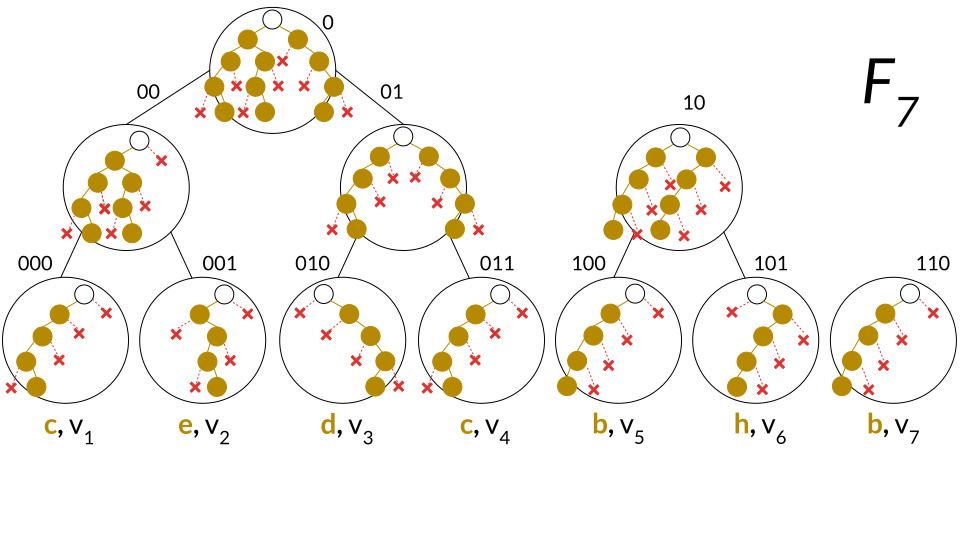
\includegraphics[width=.90\columnwidth]{figures-aad/accaad-short.pdf}
    \vspace{-1.7cm}
    \caption{
        A dynamic AAD for dictionary $\{(b,v_5),(b,v_7),(c,v_1),(c,v_4),(d,v_3),(e,v_2),(h,v_6)\}$ with $\lambda=2$.
        Unlike the AAS from \cref{f:accaas}, this AAD stores key-value pairs in the forest leaves.
        Furthermore, \textit{every node} in the forest now stores a \frontierCommunionTree (FCT).
        Similar to the AAS, all accumulators are built over the prefixes of the keys.
        This way, the accumulators can be used to ``provably-guide'' a search for all the values of a key.
    }
    \label{f:accaad-short}
\end{figure}

We can easily modify our AAS approach from \cref{s:aas:from-bilinear-acc} to obtain an AAD as depicted in \cref{f:accaad-short}.
First, the leaves in the forest will now store \textit{key-value pairs}, since we want dictionaries rather than sets.
As before, each node in the forest will store a prefix accumulator, but the accumulator will be computed only over the keys in its subtrees, even though the leaves store key-value pairs.
Thus, each tree in the forest can be regarded as a PCT, which stores key-value pairs as leaves but only accumulates the keys.
This will be very useful for proving lookups.

Second, all nodes in the forest, not just root nodes, need to store an FCT.
(In contrast, in our AAS, only root nodes stored FCTs, and internal nodes discarded them after merges.)
The FCTs enable the server to easily prove that a key $k$ is \textit{not} in a node's subtree.
This is necessary for proving lookups.
On the other hand, FCTs at every node increase the space on the server to $O(\lambda n \log{n})$.
Finally, append-only proofs remain the same as in the AAS.
We can now detail exactly how lookup proofs work.

\subsubsection{Proving Lookups}
\label{s:aad:from-acc:short:lookup-proofs}
Consider lookups for a key $k$ with a single value $v$.
Equipped with the ability of proving non-membership of $k$ in any node in the forest, the server can now easily prove such lookups.
First, the server shows $(k,v)$ is in a PCT using a proof path.
Second, to show that $k$ has no other values in that tree, the server proves $k$ is \textit{not} in any of the subtrees rooted at the sibling nodes along the proof path.
We call these subtrees \textit{missing subtrees}, since only their roots are included in the PCT proof path (as sibling nodes).
For every missing subtree, the server gives a frontier proof for $k$ not being there.
Finally, for all other PCTs in the forest, the server gives a frontier proof that $k$ is not in that PCT.

We can now generalize.
Suppose $k$ has (zero or more) values $V$ ``spread out'' across $t$ of the $O(\log{n})$ trees in the forest.
The lookup proof consists of:
\begin{itemize}
    \item For each value $v\in V$, a PCT proof path to $(k,v)$ in the forest. These paths add $O(|V|\log{n})$ overhead and form what we call a \textit{pruned forest}.
    \item For each missing subtree in this pruned forest, a frontier proof for $k$ in that subtree. There will be $O(|V|\log{n})$ such subtrees (and thus frontier proofs).
    \item For each of the $\log{(n)}-t$ remaining PCTs where $k$ has no values, a frontier proof to prove $k$ is not there. This is at most $O(\log{n})$ frontier proofs.
\end{itemize}
Thus, the lookup proof size is $O\left(|V|\log{n} + f(|V|\log{n} + \log{n})\right)$, where $f$ is the frontier proof size.
If instantiated with RSA accumulators, we call this scheme \rsaaadset, and it has $O(|V|\log{n})$ lookup proofs.
If instantiated with bilinear accumulators, we call it \biaadset, and it has $O(|V|\log^2{n})$ lookup proofs.

\subsection{AADs with Less Space Overhead}
\label{s:aad:from-acc:tall}
\begin{figure}[t]
    \centering
    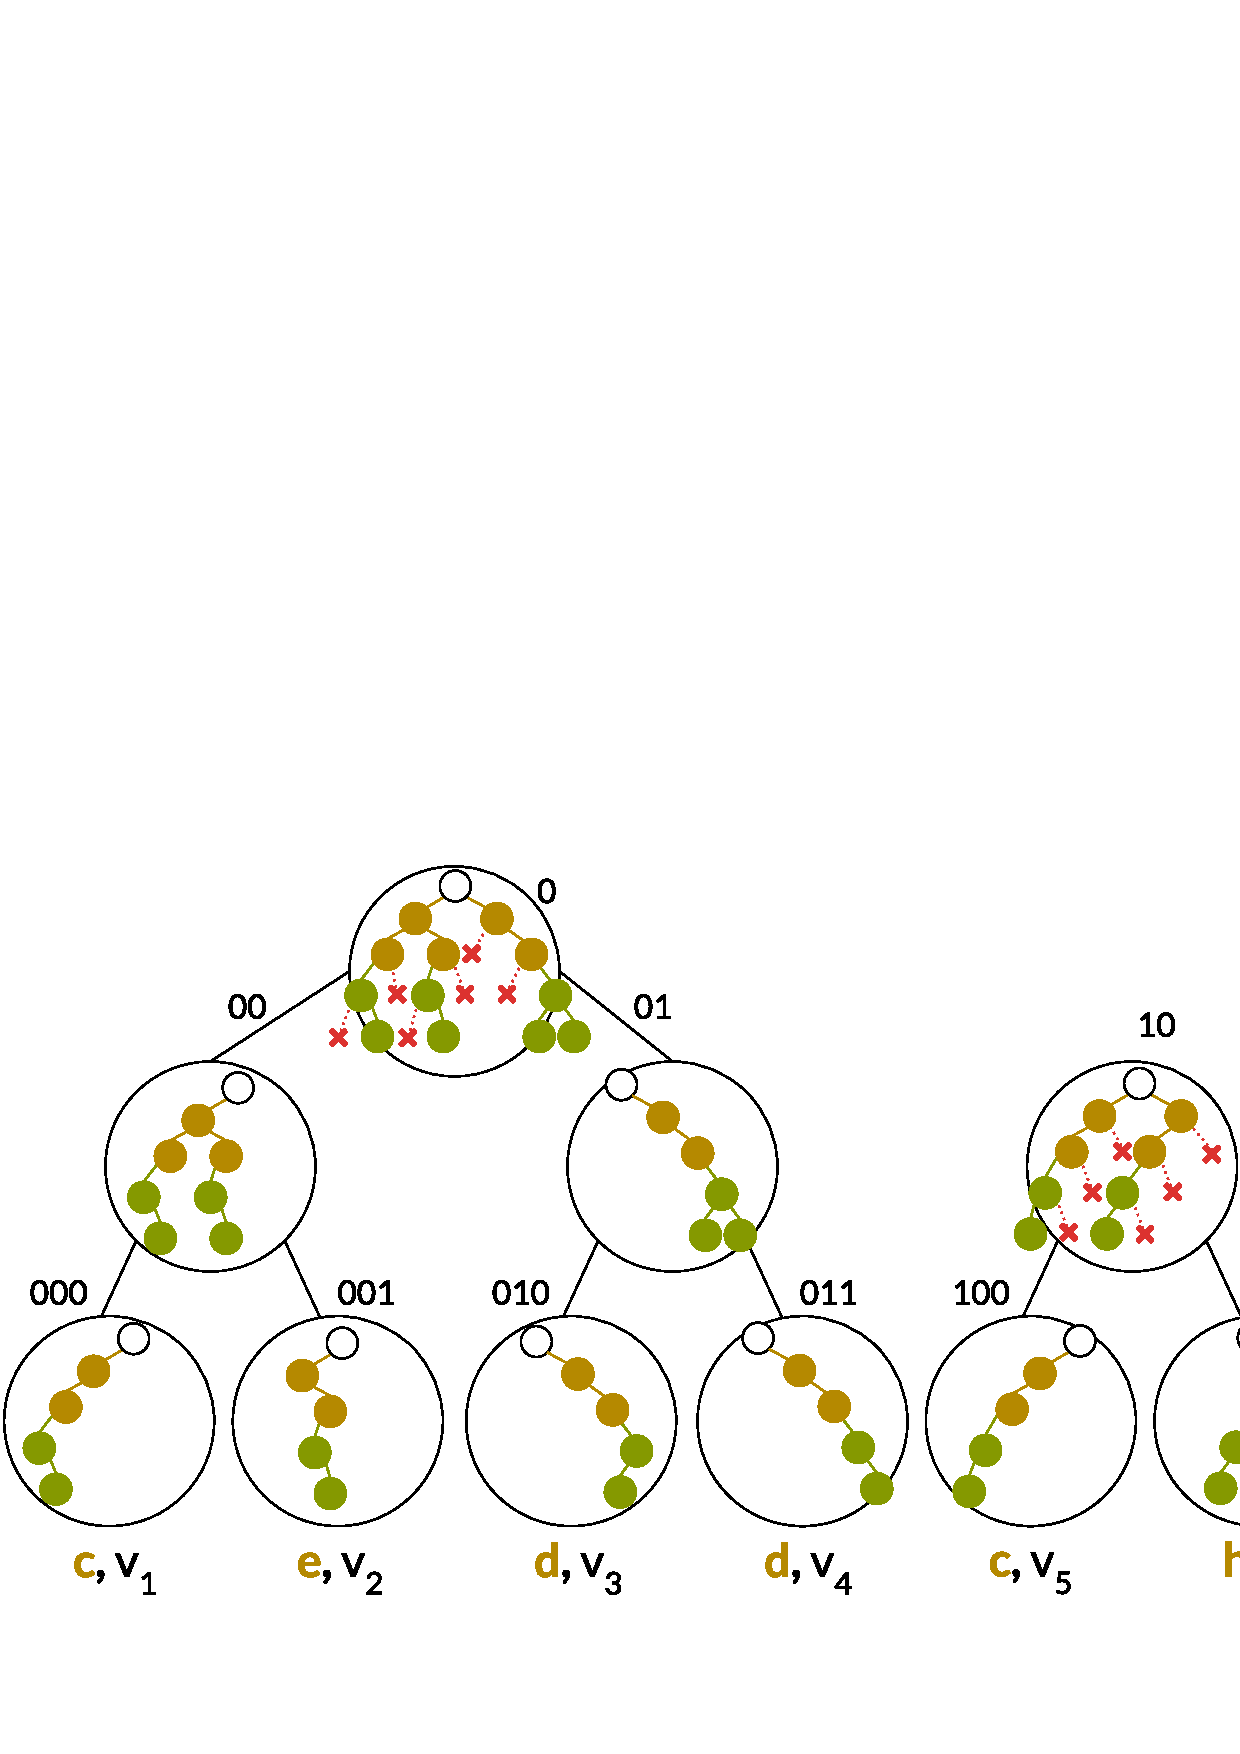
\includegraphics[width=.90\columnwidth]{figures-aad/accaad-tall.pdf}
    \vspace{-1.7cm}
    \caption{
        A dynamic AAD for dictionary $\{(c,v_1),(c,v_5),(d,v_3),(d,v_4),(e,v_2),(h,v_6),(h,v_7)\}$ with $\lambda=1$.
        The tries in this AAD are built not just over keys but also over values, unlike our AAS from \cref{f:accaas} and unlike our ``short'' AAD from \cref{f:accaad-short}.
        Specifically, the first $2\lambda$ edges in a trie path encode the hash of the key and the last $2\lambda$ edges encode the hash of the value.
        As in our AAS, \textit{only root nodes} in the forest store a \frontierCommunionTree (FCT).
        These root FCTs are used to ``provably-guide'' a search for all the values of a key.
    }
    \label{f:accaad-tall}
\end{figure}

Here, we take a different approach where PCTs accumulate both keys and their values in a manner that allows us to construct lookup proofs.
Specifically, we increase the size of the domain of the underlying AAS from $2\lambda$ bits to $4\lambda$ bits so as to account for the value $v$, as depicted in \cref{f:accaad-tall}.
That is, $(k,v)$ would be inserted in the AAS as $k|v$, using the same algorithms from \cref{s:aas:from-bilinear-acc:algorithms}.
This increases the trie height, making appends slower since more prefixes have to be accumulated.
We call the RSA-based construction \rsaaad and the bilinear-based construction \biaad.

Note that \biaad has double the $q$-PKE parameters public parameters of \biaas (and of \biaadset).
Specifically, the server needs $q=4\lambda n + 1$ and clients need $q=4\lambda+1$.
% More precisely, clients only need (g^{\tau^i})_{i\in[0,4\lambda+1]} since they never need to reconstruct extractable accumulators
On the other hand, \biaad and \rsaaad have lower space overhead than \biaadset and \rsaaad: $O(\lambda n)$ versus $O(\lambda n\log{n})$.

\paragraph{Supporting Large Domains and Multisets.}
To handle keys and values longer than $2\lambda$ bits, we store $\mathcal{H}(k)|\mathcal{H}(v)$ in the AAD (rather than $k|v$), where $\mathcal{H}$ is a CRHF and we can retrieve the actual value $v$ from another repository.
To support multisets (same $v$ can be inserted twice for a $k$), the server can insert $\mathcal{H}(\mathcal{H}(v)|i)$ for the $i$th occurrence of $(k,v)$.
% Simply inserting H(k)|H(v) does not work because if you insert (k,v) twice, and both insertions end up in the same PCT, then the frontier cannot be used to guarantee all copies of the same value $v$ have been revealed by the prover.
% In fact, the frontier is not even used here: the prover just gives a path to one of the (k,v)'s and then uses the frontier to show that there are not other values other than v for k in this PCT.
% The problem is that while that might be true, it does not say anything about how many times the value v occurrs in the PCT.

\subsubsection{Proving Lookups}
\label{s:aad:from-acc:tall:lookup-proofs}

First, consider a key $k$ with no values.
A lookup proof consists of $O(\log{n})$ frontier proofs, one for each PCT in the forest where a prefix of $k$ is missing.
This is very similar to a non-membership proof in the AAS (see \cref{s:aas:from-bilinear-acc}).

But what if $k$ has one or more values?
First, the lookup proof contains paths to PCT leaves with $k$'s values (i.e., with elements of the form $k|v$), much like a membership proof in an AAS.
But what is to guarantee \textit{completeness} of the response?
What if a malicious server leaves out one of the values of key $k$?
(This is important in transparency logs where users look up their own PKs and must receive all of them to detect impersonation attacks.)

\paragraph{Lower Frontiers.}
\begin{figure}[t]
    \centering
    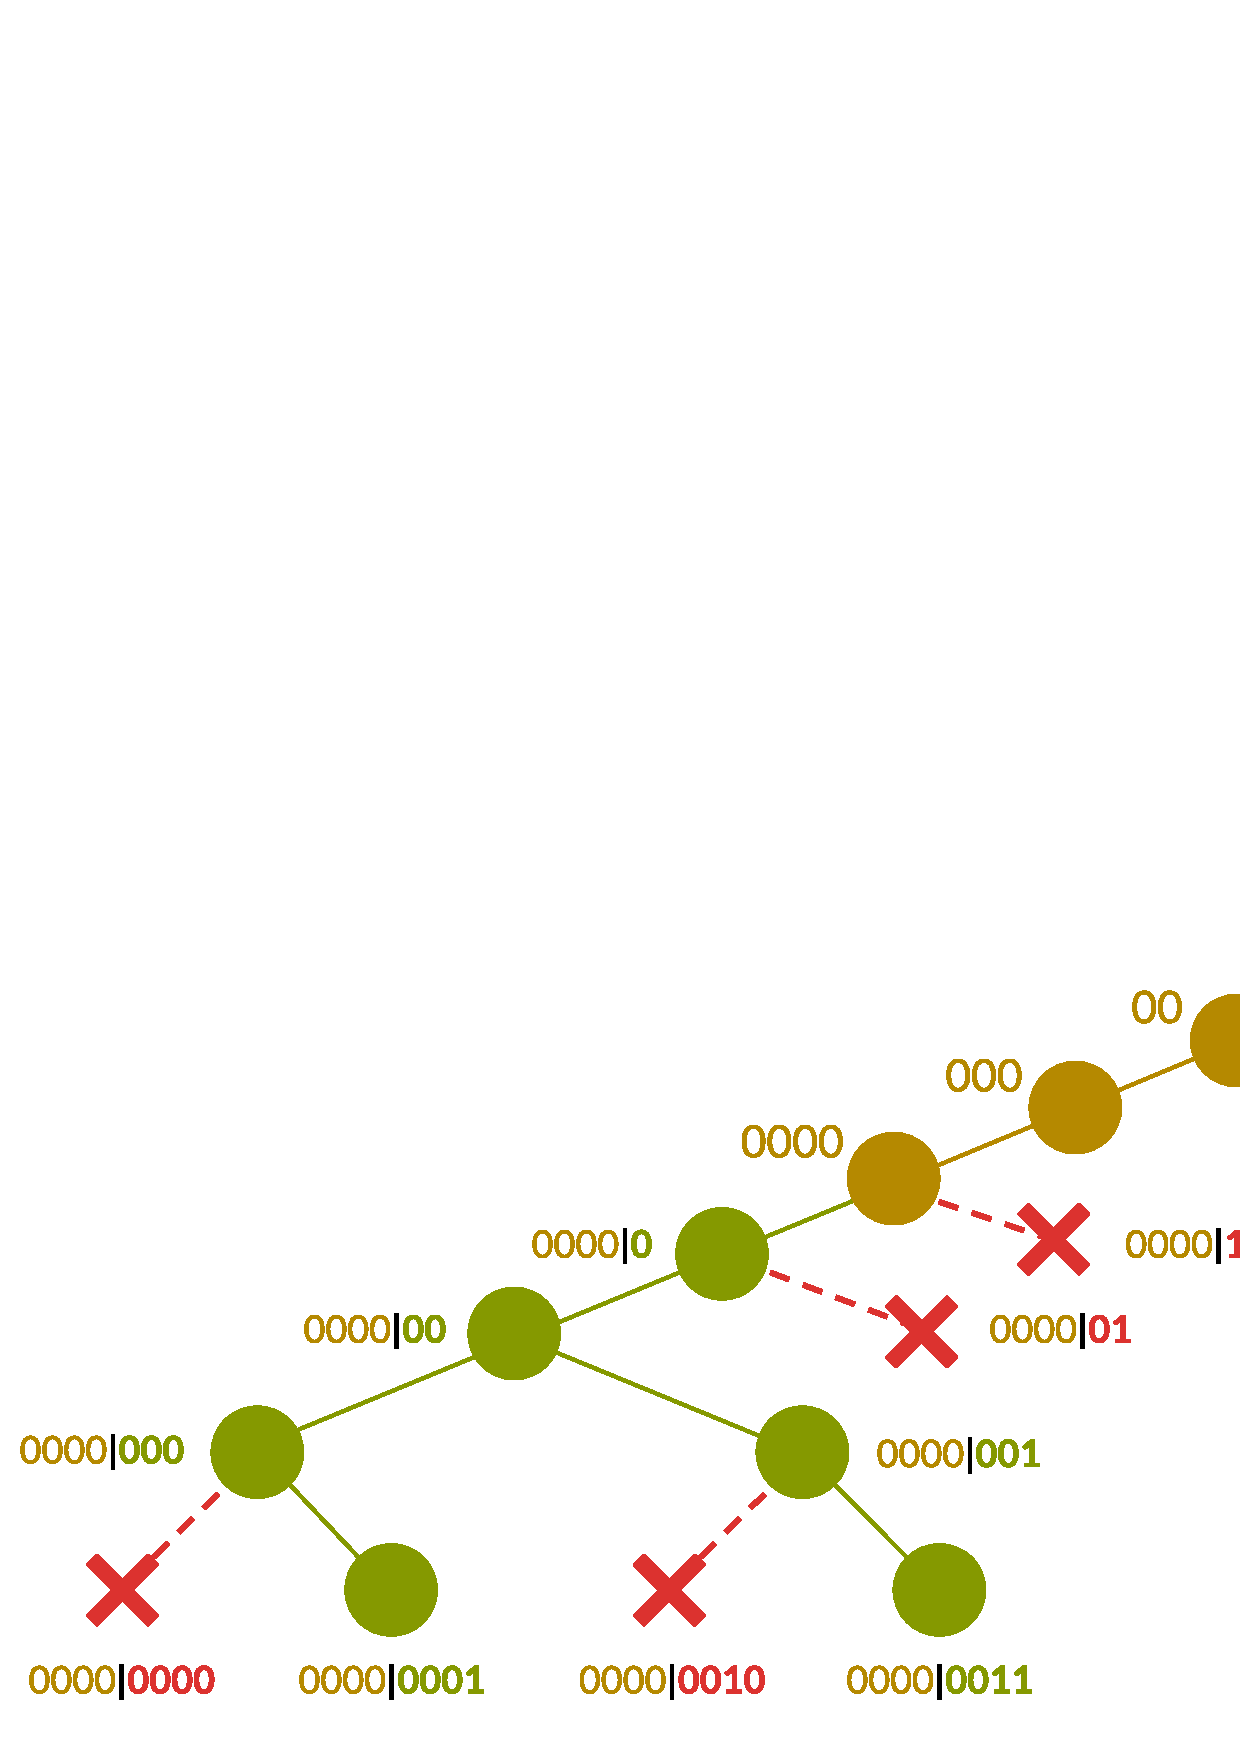
\includegraphics[width=\columnwidth]{figures-aad/lower-frontier.pdf}
    \vspace{-1.0cm}
    \caption{
        A ``tall'' trie for a key $k$ with hash $0000$ that has two values with hashes $0001$ and $0011$, respectively.
        The security parameter is $\lambda=2$.
        The lower frontier consists of the \red{red nodes} in the lower half of the trie, which correspond to missing values for $k$.
    }
    \label{f:lower-frontier}
\end{figure}
We use the same frontier technique as in the AAS to convince clients values are not being left out.
Specifically, the server proves specific prefixes for the \textit{missing values} of $k$ are not in the PCTs (and thus are not maliciously being left out).
This is best illustrated with the example in \cref{f:lower-frontier} where the security parameter is $\lambda=2$.

Suppose the server wants to prove $k=0000$ has \textit{complete} set of values $V=\{v_1 = 0001, v_2 = 0011\}$.
Consider a trie over $k|v_1$ and $k|v_2$ and note that $F^{[k]}_V = \{(0000|1), (0000|01), (0000|0000)$, $(0000|0010)\}$ is the set of all frontier prefixes for the missing values of $k$.
We call this set the \textit{lower frontier} of $k$ relative to $V$.
The key idea for showing completeness of $V$ is to \textit{prove all these lower frontier prefixes are in the FCT} via frontier proofs (as defined in \cref{s:aas:from-bilinear-acc}).
Since there are $O(\lambda)$ lower frontier prefixes, one for each value $v\in V$ of key $k$, the server will send $O(\lambda|V|)$ frontier proofs.
Thus, a proof for a key $k$ with a single value $v$ (i.e., $V=\{v\}$) consists of:
\begin{itemize}
    \item A proof path to $(k,v)$ in some PCT (to show $v$ is one of $k$'s values),
    \item $O(\lambda)$ frontier proofs in the FCT corresponding to that PCT, one for each prefix in the lower frontier $F^{[k]}_{\{v\}}$ (to guarantee completeness of $\{v\}$ in that PCT),
    \item A frontier proof for a missing prefix of $k$ in each one of the remaining $O(\log{n})$ FCTs (to prove $k$ has no values there).
\end{itemize}

\paragraph{Keys with Multiple Values.}
Let us generalize lookup proofs to keys with many values.
Assume the key $k$ has (zero or more) values in $V$ that are ``spread out'' across $t\ge 0$ of the $\le \log{n}$ PCTs in the forest.
For PCTs with no values for $k$, the server proves non-membership of $k$ in the corresponding FCT via one frontier proof.
For the $i$th PCT, where $k$ has values $v \in V_i$, the server proves the completeness of $V_i$ by giving $O(\lambda|V_i|)$ frontier proofs, one for each lower frontier prefix.
Thus, the lookup proof consists of:

\begin{itemize}
    \item For each value $v\in V$, a PCT proof path to $(k,v)$ in the forest. These add $O(|V|\log{n})$ overhead.
    \item Across the $t$ PCTs where $k$ has values, $O(\lambda|V|)$ frontier proofs will be sent.
    \item For each of the $\log{(n)}-t$ remaining PCTs where $k$ has no values, a frontier proof in its corresponding FCT to prove $k$ is not there.
\end{itemize}

Thus, the total number of frontier proofs is $O\left(\lambda|V| - t + \log{n}\right)=O\left(\lambda|V| + \log{n}\right)$.
This means the lookup proof size is $O\left(f\left(\lambda|V| + \log{n}\right) + |V|\log{n}\right)$-sized, where $f$ is the construction-specific frontier proof size.
%Now let us consider the general case of a key with values $V=\bigcup_{i\in[\log{n}]} V_i$, where $V_i$ are the values of $k$ in the $i$th tree in the forest (if any) and $t$ is the number of trees for which $V_i\ne \varnothing$.
%$O\left(\left(\sum_{i=1}^t {\lambda|V_i|}\right) - t + \log{n})\right)$ where $0 \le t\le \log{n}$.
% Because, for every tree where k has a value, the complexity goes from (\lambda + \log{n}) frontier proofs, to (\lambda + \lambda + (\log{n} - 1)) frontier proofs.
%
% All values V could be in a single tree: $O(\lambda|V|)$ frontier proofs in that tree + $O(\log{n})$ frontier proofs, one for the remaining trees
% All values V could be spread out in all trees: $O(\lambda|V|)$ frontier proofs across all tree
% Somewhere in between: $O(\lambda|V|)$ across \log{n}/2 trees + \log{n}/2 frontier proofs, one for each remaining tree
Next, we describe how to remove the $\lambda$ factor in the expression above.
% and decrease it to $O\left(f\left(|V| + \log{n}\right) + |V|\log{n}\right)$,
 
\paragraph{Smaller Lookup Proofs in \biaad.}
Since frontier proofs are $O(\log{n})$-sized, the \biaad lookup proof size will be $O(\lambda |V|\log{n}+\log^2{n})$.
% b.c., just apply $f=O(\log{n})$ in the expression from the paragraph above.
% e.g., when there are values in all trees.
% e.g., when there aren't, you have to add another \log^2{n} factor which is dominated away by \lambda\log{n}.
We show how to decrease this to $O(|V|\log{n} + \log^2{n})$.
% All values V could be in a single tree: $O(|V|\log{n})$ for that tree + $O(\log^2{n})$ for the remaining trees
% All values V could be spread out in all trees: $O(|V|\log{n})$ frontier proofs across all tree
% Somewhere in between: $O(\lambda|V|)$ across \log{n}/2 trees + \log{n}/2 frontier proofs, one for each remaining tree
We begin with the case where $k$ has one value.

We know from before that a lookup proof for $(k,\{v\})$ is $O(\lambda \log{n})$-sized
(since the $\lambda\log{n}$ term dominates the $\log^2{n}$ term).
Note that the $O(\lambda)$ overhead comes from having to prove that all $O(\lambda)$ \underline{lower} frontier prefixes of $k$ (relative to $V$) are in an FCT.
The key idea is to \textit{group all these lower frontier prefixes} into a single FCT leaf, creating a frontier accumulator over all of them.
As a result, instead of having to send $O(\lambda)$ frontier proofs (one for each lower frontier prefix), we send a single $O(\log{n})$-sized frontier proof for a single FCT leaf which contains all $O(\lambda)$ lower frontier prefixes of $k$ relative to $\{v\}$.

We can generalize this idea. 
Specifically, if $k$ has $|V_i|$ values in the $i$th FCT in the forest, then $k$'s lower frontier relative to $V_i$ has $O(\lambda|V_i|)$ prefixes.
Then, for each FCT $i$, we split the lower frontier prefixes of $k$ associated with $V_i$ into separate FCT leaves each of size at most $4\lambda + 1$.
We remind the reader that clients have enough public parameters to reconstruct the accumulators in these FCT leaves and verify the frontier proof.
% i.e., they have (g^{\tau^i})_{i=0}^{4\lambda+1}
As a result, the lookup proof size becomes $O(|V|\log{n} + \log^2{n})$.

\aadComplexityTable

\paragraph{Smaller Lookup Proofs in \rsaaad.}
Because frontier proofs are constant-sized in \rsaaas, the \rsaaad lookup proof size will be $O(\lambda |V|+\log{n}+|V|\log{n})$.
The same key idea from above can be used to bring the proof size down to $O(|V|+\log{n} + |V|\log{n})=O(|V|\log{n})$.
Recall that, in \rsaaad, constant-sized membership witnesses are computed for every frontier prefix.
Thus, in each FCT, for each key $k$'s lower frontier prefixes, we can aggregate its membership witnesses in batches of size $4\lambda+1$ using the technique from~\cite{BBF19}.

\subsection{Supporting Inclusion Proofs}
Another useful proof for a transparency log is an \textit{inclusion proof} which only returns \textit{one of the values} of key $k$ (while lookup proofs return \textit{all} values of a key $k$).
For example, in Certificate Transparency (CT), browsers are supposed to verify an inclusion proof of a website's certificate before using it.
Our AADs support inclusion proofs too.
They consist of a path to a PCT leaf with the desired key-value pair.
Since they do not require frontier proofs, inclusion proofs are only $O(\log{n})$-sized.

\subsection{Asymptotic Analysis}
\label{s:aad:from-acc:asymptotics}
We have already analyzed the lookup proof sizes of each construction in \cref{s:aad:from-acc:short:lookup-proofs,s:aad:from-acc:tall:lookup-proofs}.
The complexity analyses for the bilinear- and RSA-based AADs are similar to the ones from \cref{s:aas:from-bilinear-acc:asymptotics} and \cref{s:aas:from-rsa-acc:asymptotics}, respectively.
To avoid repetition, we give the AAD complexities in \cref{t:aad-from-acc-asymptotics}.
        
        \section{Bilinear-based AAD Implementation}
        \label{s:aad:from-bilinear-acc:eval}
        In this section, we evaluate our \biaad (not AAS) construction's proof sizes, append times and memory usage.
We find that append times and memory usage are too high for a practical deployment and discuss how they might be improved in future work (see \cref{s:eval:append-time,s:eval:memory}).
If they are improved, we find AADs can save bandwidth relative to CT and CONIKS and we describe exactly when and how much in ~\cref{s:eval:worth-it}.

\paragraph{Codebase and Testbed.}
We implemented our \textit{amortized} AAD construction from \cref{s:aad} in 5700 lines of C++.
Its \textit{worst-case} append time is $O(\lambda n \log^2{n})$ while its amortized append time is $O(\lambda \log^3{n})$.
We used Zcash's \texttt{libff}~\cite{libff} as our elliptic curve library with support for a 254-bit Barretto-Naehrig curve with a Type~III pairing~\cite{bn-curve}.
% 110 bits for BN254: https://eprint.iacr.org/2016/1102.pdf
We used \texttt{libfqfft}~\cite{libfqfft} to multiply polynomials and \texttt{libntl}~\cite{libntl} to divide polynomials and compute GCDs.
Our code is available at:
\begin{center}
    \url{https://github.com/alinush/libaad-ccs2019}.
\end{center}
We ran our evaluation in the cloud on Amazon Web Services (AWS) on a r4.16xlarge instance type with 488 GiB of RAM and 64 VCPUs, running Ubuntu 16.04.4 (64-bit).
This instance type is ``memory-optimized'' which, according to AWS, means it is ``designed to deliver fast performance for workloads that process large data sets in memory.''

\subsection{Microbenchmarks}
In this subsection, we measure:
\begin{itemize}
  \item The average time to append a key-value pair,
  \item The size of lookup proofs,
  \item The size of append-only proofs,
  \item Our memory usage.
\end{itemize}
  
\subsubsection{Append Times}
\label{s:eval:append-time}
% batch size 32
% 2019-02-04 10:50:34 36714 36714  PERF         benchAppends: 196 | Average time per append: 3422 milliseconds
% 
% batch size 64
% 2019-02-04 02:54:48 35509 35509  PERF         benchAppends: 196 | Average time per append: 3064 milliseconds
%
% batch size 128
% 2019-02-03 19:48:54 34590 34590  PERF         benchAppends: 196 | Average time per append: 2664 milliseconds
%
% batch size 256
% 2019-02-03 13:38:04 34156 34156  PERF         benchAppends: 196 | Average time per append: 2361 milliseconds
%
% batch size 512
% 2019-02-03 08:08:40 33620 33620  PERF         benchAppends: 196 | Average time per append: 1848 milliseconds
%
% batch size 1024
% 2019-02-03 03:13:40 30937 30937  PERF         benchAppends: 194 | Average time per append: 1548 milliseconds
%
% batch size 2048
% 2019-02-02 23:30:41 30167 30167  PERF         benchAppends: 194 | Average time per append: 1353 milliseconds
%
% batch size 4096
% 2019-02-02 20:15:01 29514 29514  PERF         benchAppends: 194 | Average time per append: 976 milliseconds
%
% batch size 8192
% 2019-02-02 17:47:11 28621 28621  PERF         benchAppends: 194 | Average time per append: 760 milliseconds
%

\begin{figure}[t]
    \centering
    \textbf{AAD Append Times}\par\medskip
    \includegraphics[width=.90\columnwidth,trim={0 25cm 0 0},clip]{figures-aad/aad-merged-append-time-and-proof.png}
    \caption{
        This graph plots the average append-time (y-axis) as measured after $n$ appends (x-axis).
        ``Spikes'' occur when two PCTs of size $b$ are merged in the forest (see \cref{f:forest}), which triggers a new FCT computation, where $b$ is the batch size.
        The average append time increases with the dictionary size since bigger PCTs are being created and merged (and bigger FCTs are being computed).
        Bigger batch size means PCTs are merged less frequently and FCTs are created less frequently, which decreases the average append time.
    }
    \label{f:append-time}
\end{figure}

Starting with an empty AAD, we append key-value pairs to it and keep track of the \textit{cumulative average append-time}.
Recall that appends are amortized in our construction (but can be de-amortized using known techniques~\cite{overmars-van-leeuwen,overmars}).
As a result, in our benchmark some appends are very fast (e.g., 25 milliseconds) while others are painfully slow (e.g., 1.5 hours).
To keep the running time of our benchmark reasonable, we only benchmarked $2^{13} = 8192$ appends.
We also investigate the effect of batching on append times.
Batching $k = 2^i$ appends together means we only compute one FCT for the full tree of size $k$ created after inserting the batch.
In contrast, without batching, we would compute $k$ FCTs, one for each new forest root created after an append.
\cref{f:append-time} shows that the average append time is 5.75 seconds with no batching and 0.76 seconds with batch size 8192.
(For batch sizes $32, 64, \dots, 4096$, the average times per append in milliseconds are 3422, 3064, 2644, 2361, 1848, 1548, 1353 and 976, respectively.)
These times should increase by around 3.5 seconds if we benchmarked $2^{20}$ appends.

\paragraph{Speeding Up Appends.}
The bottleneck for appends is computing the FCTs.
Although we used \texttt{libff}'s multi-threaded multi-exponentiation to compute accumulators faster, there are other ways to speed up appends that we have not explored.
First, we can parallelize computing (1) the polynomials on the same level in a FCT, (2) the smaller accumulators at lower levels of the FCT, where multi-threaded multi-exponentiation does not help as much and (3) the subset witnesses in the forest.
Second, we can reuse some of the previously computed accumulators when computing a new FCT.
Third, our PCT and FCT constructions require ``extractable'' counterparts of the accumulators, which almost triple the time to commit to a polynomial.
We hope to remove this expensive requirement by proving our construction secure in the generic group model, similar to new SNARK constructions~\cite{groth16}.
Finally, techniques for distributed FFT could speed up polynomial operations~\cite{dizk}.

\subsubsection{Lookup Proofs}
\label{s:eval:lookup}

\begin{figure*}[t]
    \centering
    \textbf{AAD Lookup Proof Size and Verification Time}\par\medskip
    \subfloat[Worst-case AAD sizes]{\label{f:lookup-worst}%
        \includegraphics[width=0.49\linewidth]{figures-aad/aad-memb-worst-case.png}
        \label{f:evaluation:lookup-worst}
    }
    \subfloat[Average-case AAD sizes]{\label{f:lookup-avg}%
        \includegraphics[width=0.49\linewidth]{figures-aad/aad-memb-avg-case.png}
        \label{f:evaluation:lookup-avg}
    }
    \caption{
        Lookup proof sizes and verification times (y-axis) increase with the dictionary size (x-axis) and with the number of values the proof attests for.
        \cref{f:lookup-worst} tells the same story as \cref{f:lookup-avg}, except the proof sizes and verification times are slightly higher since these \textit{worst-case} AADs have more trees in the forest.
    }
\end{figure*}

We investigate three factors that affect lookup proof size and verification time: (1) the dictionary size, (2) the number of trees in the forest and (3) the number of values of a key.
Our benchmark creates AADs of ever-increasing size $n$.
For speed, instead of computing accumulators, we simply pick them uniformly at random.
(Note that this does not affect the proof verification time.)
We measure \textit{average} proof sizes for keys with $\ell$ values in an AAD of size $n$, where $\ell \in \{0, 1, 2, 4, 8, 16, 32\}$.
(Recall that a key with $\ell$ values requires $\ell$ frontier proofs.)

To get an average, for every $\ell$, we set up 10 different \textit{target} keys so each key has $\ell$ values.
The rest of the inserted keys are random (and simply ignored by the benchmark).
Importantly, we randomly disperse the target key-value pairs throughout the forest to avoid having all values of a key end up in consecutive forest leaves, which would artificially decrease the proof size.
Once the dictionary reaches size $n$, we go through every target key with $\ell$ values, compute its lookup proof, and measure the size and verification time.
% (Think of a lookup proof for $\ell = 0$ values as a non-membership proof.)
Then, for each $\ell$, we take an average over its 10 target keys.
We repeat the experiment for increasing dictionary sizes $n$ and summarize the numbers in \cref{f:lookup-avg,f:lookup-worst}.
Proof verification is single-threaded.

\paragraph{Worst-Case vs. Best-Case Dictionary Sizes.}
Recall that some dictionary sizes are ``better'' than others because they have fewer trees in the forest.
For example, a dictionary of (worst-case) size $2^i - 1$ will have $i$ trees in the forest and thus $i$ FCTs.
Thus, a lookup proof must include frontier proofs in all $i$ FCTs.
In contrast, a dictionary of size $2^i$ only has a single tree in the forest, so a lookup proof needs only one {frontier proof}.
Indeed, our evaluation shows that lookup proofs are smaller in AADs of size $10^i$ (see \cref{f:lookup-avg}) compared to $2^i-1$ (see \cref{f:lookup-worst}).
For example, for a key with 32 values, the proof averages 95 KiB for size $10^6$ and 118 KiB for size $2^{20} - 1$.

%  aadSize  numValues  proofKiB    verifSecond
%  1000000          0   18.718750    0.372885
%  1000000          1   21.578125    0.446906
%  1000000          2   24.168750    0.517544
%  1000000          4   29.578125    0.661258
%  1000000          8   39.250000    0.923060
%  1000000         16   58.587500    1.452599
%  1000000         32   94.728125    2.474843

%  aadSize  numValues  proofKiB    verifSecond
%  1048575          0   41.934375    0.843512
%  1048575          1   44.803125    0.907273
%  1048575          2   47.390625    0.977507
%  1048575          4   52.418750    1.117400
%  1048575          8   62.350000    1.383276
%  1048575         16   81.684375    1.908019
%  1048575         32  118.112500    2.962104

\subsubsection{Append-only Proofs}
\label{s:eval:append-only-proof}

\begin{figure}[t]
    \centering
    \textbf{AAD Append-only Proof Size and Verification Time}\par\medskip
    \includegraphics[width=.70\columnwidth,trim={0 0 0 23cm},clip]{figures-aad/aad-merged-append-time-and-proof.png}
    \caption{
        This graph shows that our append-only proof sizes and verification times (y-axis) are quite small and scale logarithmically with the dictionary size (x-axis).
    }
    \label{f:append-only-proof}
\end{figure}

This benchmark appends random key-value pairs until it reaches a target size $n = 2^{i+1} - 1$.
Then, it measures the append-only proof size (and verification time) between AADs of size $n$ and $m = 2^{i} - 1$.
We benchmarked on $2^{i}-1$ AAD sizes to illustrate worst-case $\Theta(i)$ append-only proof sizes.
To speed up the benchmark, we randomly pick accumulators in the forest.
Append-only proof verification is single-threaded.
Our results show append-only proofs are reasonably small and fast to verify (see \cref{f:append-only-proof}).
For example, the append-only proof between sizes $2^{19}-1$ and $2^{20}-1$ is 3.5 KiB and verifies in $45$ milliseconds.

\subsubsection{Memory Usage}
\label{s:eval:memory}
% Note: The 390x is from the FrontierSizeBench numbers in experiments/ccs19/frontier-size/20
\newcommand{\frontierOverhead}{390}
Our lookup proof benchmark was the most memory-hungry: it consumed 263 GiB of RAM for an AAD of size $n = 2^{20}-1$.
In contrast, the append-only proof benchmark consumed only 12.5 GiBs of memory, since it did not need FCTs.
As an example, when $n = 2^{20} - 1$, all FCTs combined have no more than $\frontierOverhead n$ nodes.
% This would normally require $2\cdot 32 + 64 = 128$ bytes per node, but \texttt{libff} needs 96 bytes per G1 and 192 per G2 => 384 for 2*G1 + G2
Since we are using Type~III pairings, each node stores three accumulators (two in $\Group_1$ and one in $\Group_2$) in 384 bytes (due to \texttt{libff}'s 3$\times$ overhead).
Thus, the FCT accumulators require no more than 147 GiB of RAM.
% 400 * (2^20-1) * (32*2 + 64) bytes in GiB        ----> 50 GiBs     (accs ideal)
% 400 * (2^20-1) * (96*2 + 192) bytes in GiB       ----> 150 GiBs    (accs w/ libff)
% 390 * (2^20-1) * (96*2 + 192) bytes in GiB       ----> 146.24 GiBs (accs w/ libff)
%
% Each node stores: left, right, parent and data pointer: 8*4 = 32 bytes
% 390 * (2^20-1) * (8*4) bytes in GiB              ----> 12.18 GiB   (root FCT pointer overhead)
% 450 * (2^20-1) * (8*3) bytes in GiB              ----> 10.54 GiB   (root PCT pointer overhead)
The rest of the overhead comes from our pointer-based FCT implementation and other bookkeeping (e.g., polynomials).
% $q$-PKE public parameters for an AAD of size $2^{20}$ take up at least 64 GiB of RAM: 512 * 2^20 * (32 bytes * 2 + 64 bytes), ignoring libff's 3x overhead.
The $q$-PKE public parameters could have added 64 GiBs of RAM, but these two benchmarks did not need them.

\paragraph{Improving Memory.}
A new security proof could eliminate the additional $\Group_1$ and $\Group_2$ accumulators and reduce FCT memory by 2.66$\times$ and the size of the public parameters by 1.33$\times$ (see \cref{s:eval:append-time}).
% i.e., in each pair of FCT siblings, we go from 2 * [ G_1, G_1, G_2 ] (32*2 + 64 bytes) to [ G_1 ] (32 bytes) in one node and [ G2 ] (64 bytes) in the sibling (so they can be paired)
% saves 2*(32+64) / (32 + 64) = 2.66x memory
% and eliminates g_1^{\tau s^i}'s, saving (32 * 2 + 64) / (32 + 64) = 1.33x memory
A more efficient representation of group elements than \texttt{libff}'s could also reduce FCT memory by 3$\times$.
An efficient array-based implementation of PCTs and FCTs could further reduce memory by tens of gigabytes.
Finally, the 390$\times$ overhead of FCTs can be drastically reduced by carefully grouping upper frontier prefixes together in a FCT leaf, similar to the grouping of lower frontier prefixes from \cref{s:aad}.
However, doing this without increasing the lookup proof size too much remains to be investigated.
% The idea is that right now, each upper frontier prefix gets its own FCT leaf.
% This is because when proving non-membership of a key, we have to give a frontier proof for one of its missing prefixes.
% We do this by giving a subset path to a FCT leaf containing \textit{just} that missing prefix.
% But this means we incur a large computational overhead, creating roughly 2\lambda leaves for every newly inserted key's upper frontier prefixes.
% We could reduce this drastically by grouping upper frontier prefixes too (similar to how we group lower frontier prefixes).
% The downside is that, now, a frontier proof for an upper frontier prefix will be sending a path to a leaf with several other prefixes.
% To verify the leaf accumulator of this path, the verifier will have to recreate it from scratch.
% So he will need to be given the other/extra upper frontier prefixes in that leaf.
% This will slightly increase proof sizes, but could be mitigated against with compression.

\subsection{Comparison to Merkle Tree Approaches}
\label{s:eval:comparison-to-merkle}

How do AADs compare to Merkle prefix trees or History Trees (HTs), which are used in CONIKS and Certificate Transparency (CT), respectively?
First of all, appends in AADs are orders of magnitude slower because of the overheads of cryptographic accumulators and remain to be improved in future work (see \cref{s:eval:append-time}).

Lookup proofs in prefix trees are much smaller than in AADs.
% $\log_2(2^{20}) \cdot 32 = 640$ bytes
In a prefix tree of size $2^{20}$, a proof consisting of a Merkle path would be around $640$ bytes.
In comparison, our proofs for a key with 32 values are 152 times to 189 times more expensive (depending on the number of trees in the forest).
% 95 KiB / 640 bytes = 152x
% 118 KiB / 640 bytes = 189x
On the other hand, append-only proofs in AADs are $O(\log{n})$, much smaller than the $O(n)$ in prefix trees.
For example, our Golang implementation of prefix trees, shows that the append-only proof between trees of size $2^{19}$ and $2^{20}$ is 32 MiB (as opposed to 3.5 KiB in AADs).
The proof gets a bit smaller when the size gap between the dictionaries is larger but not by much: 14.6 MiB between $10^5$ and $10^6$.

Lookup proofs in history trees (HTs) are $O(n)$-sized, compared to $O(\log^2{n})$ in AADs.
This is because, to guarantee completeness, the HT proof must consist of all key-value pairs.
On the other hand, append-only proofs in AADs are slightly larger than in HTs.
While our proofs contain approximately the same number of nodes as in HT proofs, our nodes store two prefix accumulators in $\Group_1$ and a subset witness in $\Group_2$ (in addition to a Merkle hash).
This increases the per-node proof size from 32 bytes to 32 + 64 + 64 = 160 bytes.

% Sparse Merkle prefix tree proof sizes
% oldSize   newSize     appendOnlyProfSize
% 524,288   1,048,576   32 MiB
% 100,000   1,000,000   14.3 MiB

% Append-only proof sizes:
%  newDictSize  proofKiB  verifyMillisec
%         1023     1.59375      21.521
%         2047     1.78125      24.105
%         4095     1.96875      26.698
%         8191     2.15625      29.022
%        16383     2.34375      31.749
%        32767     2.53125      34.103
%        65535     2.71875      36.689
%       131071     2.90625      38.830
%       262143     3.09375      40.976
%       524287     3.28125      43.664
%      1048575     3.46875      45.573


\subsubsection{When do AADs Reduce Bandwidth?}
\label{s:eval:worth-it}
Asymptotically, AAD proof sizes outperform previous work.
But in practice, our evaluation shows AAD proof sizes are still larger than ideal, especially lookup proofs.
This begs the question: \textit{In what settings do AADs reduce bandwidth in transparency logs?}
We answer this question below while acknowledging that AAD append times and memory usage are not yet sufficiently fast for a practical deployment (see \cref{s:eval:append-time}).

To begin, consider a key transparency log with approximately one billion entries (i.e., an entry is a user ID and its PK).

\newcommand{\coniksfreq}{\ensuremath{\mathbf{\mathsf{D}}}\xspace}
\newcommand{\checkfreq}{\ensuremath{\mathbf{\mathsf{C}}}\xspace}

\paragraph{CONIKS.}
In a CONIKS log, each user must check their PK in every digest published by the log server.
Let \coniksfreq denote the number of digests published per day by the log server.
This means the CONIKS log server will, on average, send $960 \cdot \coniksfreq$ bytes per day per user (without accounting for the overhead of VRFs~\cite{vrf} in CONIKS).
If this were an AAD log, then each user (1) gets the most recent digest via an append-only proof and (2) checks their PK only in this digest via a lookup proof.

Let \checkfreq denote the number of times per day a user checks his PK (and note that, in CONIKS, $C = D$).
Since the lookup proof is for the user's PKs not having changed, it only needs to contain frontier proofs.
Extrapolating from \cref{f:lookup-avg}, such an average-case lookup proof is 40 KiB (in an AAD of size one billion).
Similarly, an append-only proof would be 7 KiB.
This means the AAD log server will, on average, send $47 \cdot 1024 \cdot C$ bytes per day per user.
Thus, AADs are more efficient when $.0199 \cdot D / C > 1$.

% Thus, if $C < (960 \cdot D) / (47\cdot 1024) =  0.0199 \cdot D$, then the AAD log server requires less bandwidth than CONIKS.
In other words, AADs will be more bandwidth-efficient in settings where log digests must be published frequently (i.e., $D$ is high) but users check their PK sporadically (i.e., $C$ is low).
% This should already be the case in key transparency, where all users should be able to register and update keys quickly (for availability reasons) even though some users might check their keys less often (since users can be offline).
For example, if $D=250$ (i.e., a new digest every 6 minutes) and $C=0.5$ (i.e., users check once every two days), then AADs result in 10$\times$ less bandwidth.

%% In CT, the server has to send   (certs_per_sec * cert_size_bytes * num_monitors)               bytes / sec
%% In AADs, the server has to send (47 * 1024 / (3600 * 24) * num_monitors * monitorings_per_day) bytes / sec
%%                                  .557 * num_monitors * monitorings_per_day)                    bytes / sec
%%
%% CT / AAD bandwidth overhead: 
%%      certs_per_sec * cert_size_bytes / (.557 * monitorings_per_day)
%%      17318 / (.557 monitorings_per_day)
%%      e.g., 1295.481 when monitoring once per hour (which is consistent with 483 GiBps / 383 MiBps)
%%
%% As long as:
%%      monitorings_per_day < certs_per_sec * cert_size_bytes / (47*1024/(3600*24))
%%      monitorings_per_day < certs_per_sec * cert_size_bytes / .557
%%      monitorings_per_day < 31,091.56
%% ...AADs result in less bandwidth.
\paragraph{Certificate Transparency (CT).}
Recall that CT lacks succinct lookup proofs.
As a result, domains usually trust one or more \textit{monitors} to download the log, index it and correctly answer lookup queries.
Alternatively, a domain can act as a monitor itself and keep up with every update to the log.
We call such domains \emph{monitoring domains}.

Currently, CT receives 12.37 certificates per second on average~\cite{ct-num-certs}, with a mean size of 1.4 KiB each~\cite{ct-avg-cert-size}.
Thus, a CT log server will, on average, send $12.37 \cdot 1.4 \cdot 1024 = 17,733.63$ bytes per second per monitoring domain.
In contrast, AADs require $47 \cdot 1024 \cdot C / 86,400 = .557\cdot C$ bytes per second per monitoring domain.
As before, $C$ denotes how many times per day a monitoring domain will check its PK in the log.
Thus, AADs are more efficient when $31,837 / C > 1$.

So even if domains monitor very frequently (e.g., $C = 100$), AADs are more bandwidth efficient.
However, we stress that our append times and memory usage must be reduced for a practical deployment to achieve these bandwidth savings (see \cref{s:eval:append-time,s:eval:memory}).

%% CONIKS bandwidth
%  ----------------
% Assume the CONIKS log publishes 10,000 digests per day.
% bytes_per_user = 960 bytes * 10,000 / day = 111.11 bytes/user/sec
% bytes_total = 111.11 bytes/user/sec * 1,000,000,000 = 103 GiBps
%
% If the frequency is to update the log once per hour, then CONIKS beats AADs.
% 960 bytes * 24 / day = 0.266666667 bytes/user/sec
% multiplied by 1,000,000,000 users, that's 254.31 MiBps.
% If it's once per minute, then the bandwidth would go to 253.31 MiBps * 60 = 14.9 GiBps.
% On the other hand, the proofs can be compressed using diffs, which could save a lot of traffic.

%% AAD bandwidth for CONIKS
%  ------------------------
% 47 KiB 10^9 / day = 47 KiB * 1024 bytes/KiB * 10^9 users / (24 hr/day * 60 min/hr * 60 sec/min) = 557037037 bytes/sec = 531.23 MiBps

%% CT bandwidth
%  ------------
% First CT log was launched in March 2013. Today is July 7, 2018 ([source](https://en.wikipedia.org/wiki/Certificate_Transparency#Certificate_authority_implementation))
% 1976 days between 03/01/2013 and 07/28/2018
% 2,112,278,786 certificates
% 1068966 certs/day
% 12.37 certs/second
% 1,400 bytes: the average size of a certificate
% 12.37 certs/sec * 1,400 bytes/cert = 17,318 bytes/sec
% 17,318 bytes/sec * 30 million = 519540000000 bytes/sec =  483 GiB/sec if 30 million domains monitor

%% AAD bandwidth for CT
%  --------------------
% 47 KiB * 1024 bytes/KiB * 30 million domains / hr = (47 * 1024 * 30*10^6 / 3600) / sec = 401,066,666.667 bytes/second = 383 MiBps

%
% Part II: AMT [VSS/DKG]
%
\part{Threshold Cryptosystems}
\label{s:threshcrypto}

    
    \chapter{Introduction}
    \label{s:threshcrypto:intro}
    \newcommand{\vssDkgPreviousWorkTable}{
\begin{table}[h]
    %\large
    %\small
    \footnotesize
    %\scriptsize
    \centering
    %\vspace{1em}
    %\vspace{2.2em}
    \begin{tabular}{lcccccc}
        %\toprule
        {\makecell{Scheme}}
        & \makecell{Dealing\\round\\time}
        & \makecell{Verification\\round\\time}
        & \makecell{Complaint\\round\\time}
        & \makecell{Reconstruct\\time\\(no interpol.)}
        & \makecell{Dealing\\communic.\\(broadcast)}
        & \makecell{Dealing\\communic.\\(private)}\\
        \toprule

        Feldman VSS~\cite{Feldman87} & $n\log{n}$   & $t$          & \myred{$t^2$} & \myred{$nt$} & \myred{$t$} & $n$ \\
        \jfdkg~\cite{GJKR07}         & $n\log{n}$   & \myred{$nt$} & \myred{$t^3$} & \myred{$nt$} & \myred{$t$} & $n$ \\
        \evss ~\cite{KZG10a}         & \myred{$nt$} & $1$          & $t$           & $n$          & $1$         & $n$ \\
        \ejfdkg~\cite{Kate2010}      & \myred{$nt$} & $n$          & \myred{$t^2$} &$n$           & $1$         & $n$ \\

        \toprule

        \textbf{\ourvss}   & $n\log{t}$ & $\log{t}$  & $t\log{t}$           & $n\log{t}$ & $1$ & $n\log{t}$ \\
        \textbf{\ourdkg}   & $n\log{t}$ & $n\log{t}$ & \myred{$t^2\log{t}$} & $n\log{t}$ & $1$ & $n\log{t}$ \\
    \end{tabular}
    \caption{
       Per-player \textit{worst-case} asymptotic complexity of $(t,n)$ VSS/DKG protocols.
    }
    \label{t:vss-dkg-comparison} % must go after \caption{} for \cref{} to work
    %\toprule
\end{table}
}

% For more motivation, see intro of: [ZI03] "Round optimal distributed key generation of threshold cryptosystem based on discrete logarithm problem"
% "A great proportion of solutions to multiparty protocols turns out to be a crux of threshold cryptosystem scheme in constructing a distributed TTP: key recovery [24], signature escrow [15,23], contract signing [27], fair exchange of digital signatures [2], e-voting [9,19] and auction [6] schemes."

Due to the popularity of cryptocurrencies, interest in Byzantine fault tolerant (BFT) systems has been steadily increasing~\cite{bitcoin,ethereum,GAG+19,algorand,dfinity,ouroboros,ouroboros-praos,ouroboros-genesis,randherd}.
At the core of BFT systems often lie simpler threshold cryptosystems such as threshold signature schemes (TSS)~\cite{Boldyreva03,Shoup00}, verifiable secret sharing (VSS) protocols~\cite{Pedersen1991NonInteractive,CGMA85,KZG10a} and distributed key generation (DKG) protocols~\cite{Pedersen1991AThreshold,GJKR07,Kate2010}.
For example, TSS and DKG protocols are used to scale consensus protocols~\cite{GAG+19,dfinity,constantinople}.
Furthermore, DKG protocols~\cite{GJKR07} are used to securely generate keys for TSS~\cite{KG09}, to generate nonces for interactive TSS~\cite{SS01,GGN16}, and to build proactively-secure threshold cryptosystems~\cite{Herzberg1995ProactiveSecret,Herzberg1997ProactivePublic}.
Finally, VSS is used to build multi-party computation (MPC) protocols~\cite{GRR98p}, random beacons~\cite{randherd,CD17a,ouroboros} and is the key component of DKG protocols.

Despite their usefulness, TSS, VSS and DKG protocols do not scale well in important settings.
For example, BFT systems often operate in the \textit{honest majority} setting, with $n$ total players where $t > n/2$ players must be honest.
In this setting, \textit{$t$-out-of-$n$ threshold cryptosystems}, such as TSS, VSS and DKG, require time quadratic in $n$~\cite{Feldman87,Pedersen1991NonInteractive,KZG10a,Boldyreva03}.
This is because of two reasons.
% Note: At this point, it might not be clear to all readers that threshold cryptosystems reconstruct secrets, so we clarify below.
First, reconstruction of secrets, a key step in any threshold cryptosystem, is typically implemented naively using $\Theta(t^2)$ time polynomial interpolation, even though faster algorithms exist~\cite{vG13ModernCh10}.
This makes aggregating threshold signatures and reconstructing VSS or DKG secrets slow for large $t$.
Second, either the dealing round, the verification round or the reconstruction phase in VSS and DKG protocols require $\Theta(nt)$ time.
% e.g., Feldman VSS has $\Theta(nt)$ worst-case time to verify shares during reconstruction.
Fundamentally, this is because current polynomial commitment schemes require $\Theta(nt)$ time to either compute or verify all proofs~\cite{Feldman87,Pedersen1991NonInteractive,KZG10a}.
In this thesis, we address both of these problems.

\paragraph{Contributions.}

Our first contribution is a BLS TSS~\cite{Boldyreva03} with $\Theta(t\log^2{t})$ aggregation time, $\Theta(1)$ signing and verification times and $\Theta(1)$ signature size (see \cref{s:threshsig}).
In contrast, previous schemes had $\Theta(t^2)$ aggregation time (see \cref{s:related-work:tss}).
We implement our fast BLS TSS in C++ and show it outperforms the naive BLS TSS as early as $n\ge \blsOutperformN$ and scales to $n$ as large as 2 million (see \cref{s:eval:threshsig}).
At that scale, we can aggregate a signature \blsTimeImprovFriendly{2097151} faster in \blsEffTimeFriendly{2097151} compared to \blsNaiveTimeFriendly{2097151} if done naively.
Our fast BLS TSS leverages a $\Theta(t\log^2{t})$ time \textit{fast Lagrange} interpolation algorithm~\cite{vG13ModernCh10}, which outperforms the $\Theta(t^2)$ time \textit{naive} \textit{Lagrange} algorithm.

\vssDkgPreviousWorkTable

Our second contribution is a space-time trade-off for computing evaluation proofs in \textit{KZG polynomial commitments}~\cite{KZG10a} (see \cref{s:amt}).
KZG commitments are quite powerful in that their size and the time to verify an evaluation proof are both constant and do not depend on the degree of the committed polynomial.
We show how to compute $n$ evaluation proofs on a degree $t$ polynomial in $\Theta(\amtDealTime)$ time.
Each proof is of size $\floor{\log{t}}-1$ group elements.
Previously, each proof was just one group element but computing all proofs required $\Theta(nt)$ time.
Our key technique is to authenticate a polynomial multipoint evaluation at the first $n$ roots of unity (see \cref{s:prelim:fft}), obtaining an \textit{authenticated multipoint evaluation tree (AMT)}.
Importantly, similar to KZG proofs, our AMT proofs remain homomorphic (see \cref{s:scalable-dkg:homomorphic-amt}), which is useful when we apply them to distributed key generation (DKG) protocols.
Finally, AMTs give rise to a new \textit{vector commitment (VC)} scheme~\cite{CF13,CPZ18} as we discuss in \cref{s:vcs:from-amt}.

Our third contribution is \ourvss, a scalable VSS with a $\Theta(n\log{t})$ time sharing phase, an $O(t\log^2{t}+n\log{t})$ time reconstruction phase, $\Theta(1)$-sized broadcast (during dealing round) and $\Theta(n\log{t})$ overall communication.
% Note: Dealer broadcasts a KZG commitment during dealing and { batch proof (or < t KZG proofs) + < t shares } during the complaint round
\ourvss improves over previous VSS protocols which, in the worst case, incur $\Theta(nt)$ computation.
However, this improvement comes at the cost of slightly higher verification times and communication (see \cref{t:vss-dkg-comparison}).
Nonetheless, in \cref{s:threshcrypto:eval}, we show \ourvss outperforms \evss~\cite{KZG10a}, the most communication-efficient VSS, as early as $n=\vssOutperformBcN$. 
Importantly, \ourvss is highly scalable. 
For example, for $n\approx 2^{17}$, we reduce the best-case end-to-end time of \evss from \evssVssEndToEndBcTimeFriendly{131071} to \amtVssEndToEndBcTimeFriendly{131071}.

Our fourth contribution is \ourdkg, a DKG with a $\Theta(n\log{t})$ time sharing phase (except for its quadratic time complaint round), an $O(t\log^2{t}+n\log{t})$ time reconstruction phase, a $\Theta(1)$-sized broadcast (during dealing round) and $\Theta(n\log{t})$ per-player dealing communication.
\ourdkg improves over previous DKGs which, in the worst case, incur $\Omega(nt)$ computation.
% Specifically:
%  - in JF-DKG, dealing is efficient, best-case verification is efficient, but worst-case reconstruction is inefficient
%  - in eJF-DKG, dealing is inefficient
%  - in AMT DKG, everything is efficient
Once again, this improvement comes at the cost of slightly higher verification times and communication (see \cref{t:vss-dkg-comparison}).
Nonetheless, in \cref{s:threshcrypto:eval}, we show \ourdkg outperforms \ejfdkg~\cite{Kate2010}, the most communication-efficient DKG, as early as $n=\dkgOutperformBcN$.
% Note: AMT VSS is slower than AMT DKG in the ``best case'' due to best-case VSS reconstruction needing to verify $t$ shares.
For $n\approx 2^{17}$, we reduce the best-case end-to-end time of \ejfdkg from \ejfDkgEndToEndBcTimeFriendly{131071} to \amtDkgEndToEndBcTimeFriendly{131071}.

Our last contribution is an open-source implementation:
\begin{center}
\url{https://github.com/alinush/libpolycrypto/}
\end{center}

\paragraph{Limitations.}
Our work only addresses TSS, VSS and DKG protocols secure against \textit{static} adversaries.
% WARNING: I keep forgetting that NBB16 withstands only static adversaries.
% WARNING: SJSW19 says they are adaptively-secure but I don't see an argument as to why/how.
However, \textit{adaptive security} can be obtained, albeit with some overheads\cite{CGJ+99,Feldman87,AF04,FMY99,JL00}.
We only target \textit{synchronous} VSS and DKG protocols, which make strong assumptions about the delivery of messages.
However, recent work~\cite{SJSW19} shows how to instantiate such protocols using the Ethereum blockchain~\cite{ethereum}.
Our VSS and DKG protocols require a \textit{trusted setup} (see \cref{s:prelim:trusted-setup}).
Our evaluation only measures the computation in VSS and DKG protocols and does not measure network delays that would arise in a full implementation on a real network.
Our techniques slightly increase the communication overhead of VSS and DKG protocols from $\Theta(n)$ to $\Theta(n\log{t})$.
However, when accounting for the time savings, the extra communication is worth it.
Still, we acknowledge communication is more expensive than computation in some settings.
Finally, we do not address the worst-case quadratic overhead of complaints in DKG protocols.
We leave scaling this to future work.
        
        \section{Related Work}
        \label{s:threshcrypto:related-work}
        % Desmedt and Frankel~\cite{DesmedtFrankel1990Threshold} were the first to instantiate threshold encryption using ElGamal encryption~\cite{ElGamal1985APublicKey} and Shamir secret sharing~\cite{how-to-share-a-secret}.
% Later on, Desmedt and Frankel~\cite{DesmedtFrankel1992SharedGeneration} introduced the first RSA-based threshold signature.
% Shoup introduced a more practical RSA-based threshold signature~\cite{Shoup2000Practical}.
% Harn introduced the first ElGamal-based threshold signature~\cite{Harn1994GroupOriented}.

\subsection{Threshold Signature Schemes (TSS)}
\label{s:related-work:tss}

Threshold signatures and threshold encryption were first conceptualized by Desmedt~\cite{Desmedt87}, who proposed inefficient constructions based on generic multi-party computation (MPC) protocols~\cite{GMW87}.
Desmedt and Frankel later efficiently instantiated these ideas via a threshold-variant of ElGamal encryption~\cite{DF90}.
Since then, many threshold signatures based on \textit{Shamir secret sharing} (see \cref{s:prelim:vss}) have been proposed~\cite{DesmedtFrankel1992SharedGeneration,Shoup00,Harn94,GJKR96,SS01,Boldyreva03,GGN16,PK96}.
To the best of our knowledge, none of these schemes addressed the $\Theta(t^2)$ time required for polynomial interpolation.
Furthermore, all current BLS TSS~\cite{Boldyreva03} implementations seem to use this quadratic algorithm~\cite{bls-chia-impl,bls-sbft-impl,bls-dfinity-impl,bls-herumi-impl} and thus do not scale to large $t$.
In contrast, our work uses $\Theta(t\log^2{t})$ fast Lagrange interpolation and scales to $t = 2^{20}$ (see \cref{s:threshsig}).

An alternative to a TSS is a \textit{multi-signature scheme (MSS)}.
Unlike a TSS, an MSS does not have a unique, constant-sized public key (PK) against which all final signatures can be verified.
Instead, the PK is dynamically computed given the contributing signers' IDs and their public keys.
This means that a $t$-out-of-$n$ MSS must include the $t$ signer IDs as part of the signature, which makes it $\Omega(t)$-sized.
Furthermore, MSS verifiers must have all signers' PKs, which are of $\Omega(n)$ size.
To fix this, the PKs can be Merkle-hashed but this now requires including the PKs and their Merkle proofs as part of the MSS~\cite{STV+16}.
(This communication overhead can be addressed by using a more communication-efficient vector commitment scheme~\cite{CF13}, but only by introducing additional computational overhead.)
On the other hand, an MSS is much faster to aggregate than a TSS.
Still, due to its $\Omega(t)$ size, an MSS does not always scale.

\subsection{Verifiable Secret Sharing (VSS)}
\label{s:related-work:vss}
VSS protocols were introduced by Chor et al.~\cite{CGMA85}.
Feldman proposed the first efficient, non-interactive VSS with computational hiding and information-theoretic binding~\cite{Feldman87}.
Pedersen introduced its counterpart with information-theoretic hiding and computational binding~\cite{Pedersen1991NonInteractive}.
Both schemes require a $\Theta(t)$-sized broadcast during dealing.

Kate et al.'s \evss reduced this to $\Theta(1)$ using constant-sized polynomial commitments~\cite{KZG10a}.
\evss also reduced the verification round time from $\Theta(t)$ to $\Theta(1)$.
However, \evss's $\Theta(nt)$ dealing time scales poorly when $t\approx n$.
Our work improves \evss to $\Theta(\amtDealTime)$ dealing time at the cost of \amtOneShareVerifTime verification round time.
We also increase communication from $\Theta(n)$ to \amtAllShareVerifTime (see \cref{t:vss-dkg-comparison}).
%(The dealing time in Feldman's and Pedersen's VSS is $\Theta(n\log{n})$ because they must evaluate a degree $t-1$ polynomial at $n$ points, which they can do with an FFT.)
% While Pedersen and Feldman's VSS incurred $\Theta(nt)$ time for all players to verify their shares, Kate et al.'s VSS just shifts this cost to the dealer.

\subsection{Publicly-Verifiable Secret Sharing (PVSS)}
\label{s:related-work:pvss}

Stadler proposed publicly verifiable secret sharing (PVSS) protocols~\cite{Stadler1996Publicly} where any \textit{external verifier} can verify the VSS protocol execution.
As a result, PVSS is less concerned with players individually and efficiently verifying their shares, instead enabling external verifiers to verify all players' (encrypted) shares.
Schoenmakers proposed an efficient $(t,n)$ PVSS protocol~\cite{Schoenmakers1999} where dealing is $\Theta(n\log{n})$ time and external verification of all shares is $\Theta(nt)$ time, later improved to $\Theta(n)$ time by Cascudo and David~\cite{CD17a}.
Unfortunately, when the dealer is malicious, PVSS still needs $\Theta(nt)$ computation during reconstruction.
Furthermore, PVSS might not be a good fit in protocols with a large number of players.
In this setting, it might be better to base security on a \textit{large}, threshold number of honest players who individually and efficiently verify their own share rather than on a \textit{small} number of external verifiers who must each do $\Omega(n)$ work.
Indeed, recent work explores the use of VSS within BFT protocols \textit{without} external verifiers~\cite{BTA+19}.
Nonetheless, our \ourvss protocol can be easily modified into a PVSS since an AMT for all $n$ proofs can be batch-verified in $\Theta(n)$ time (see \cref{s:scalable-vss:reconstruction}).

% Note: First person to pose the DKG question was C. Meadows in "Some Threshold Schemes Without Central Key Distributors", in CRYPTO 1988 (I think) or in "Congressus Numerantium, 46, 1985, pp. 187-199." but cannot find the paper online.
\subsection{Distributed Key Generation (DKG)}
\label{s:related-work:dkg}
DKG protocols were introduced by Ingemarsson and Simmons~\cite{Ingemarsson1991} and subsequently improved by Pedersen ~\cite{Pedersen1991AThreshold,Pedersen1991NonInteractive}.
Gennaro et al.~\cite{GJKR07} noticed that if players in Pedersen's DKG refuse to deal~\cite{Pedersen1991AThreshold}, they cannot be provably blamed and fixed this in their new \jfdkg protocol.
They also showed that secrets produced by Pedersen's DKG can be \textit{biased}, and fixed this in their \newdkg protocol.
% Note: Gennaro's unbiasable New-DKG with Pedersen commitments can be made more efificient (one less round, I think) by changing the reconstruction of $y=g^z_i$ to use proofs-of-knowledge~\cite{Canetti1999Adaptive}.
% But, NBB16 is even better I think.
Neji et al. gave a more efficient way of debiasing Pedersen's DKG~\cite{NBB16}.
Gennaro et al. also introduced the first ``fast-track'' or optimistic DKG~\cite{GRR98p}.
Canetti et al. modified \newdkg into an adaptively-secure DKG~\cite{CGJ+99}.
Fouque and Stern~\cite{FS01} gave a one-round DKG that removes the need for an expensive \textit{complaint round} (see \cref{alg:dkg}).
So far, all DKGs required a $\Theta(t)$-sized broadcast by each player.
% Note: In the worst case, \ejfdkg requires $\Theta(f^2)$ pairings to verify $\Theta(f^2)$ complaints.
% Even worse, JF-DKG would require $\Theta(f^2 \times t)$ time.

% Notes:
%  - Kate et al. DKG papers don't mention eJF-DKG. 
%  - PolyCommit mentions that eVSS can be applied to DKG, but does not explore the NIZKs needed to prove g^{f_i(0)} is correct.
%  - So attribution goes to Kate's thesis.
Kate's \ejfdkg~\cite{Kate2010} reduced the dealer's broadcast to $\Theta(1)$ via constant-sized polynomial commitments~\cite{KZG10a}, taking a first step towards scalability.
% Note: DKG verification of $n$ shares in JF-DKG is $nt$ exponentiations in the worst case.
\ejfdkg also reduced verification time from $\Theta(nt)$ per player to $\Theta(n)$ but at the cost of $\Theta(nt)$ dealing time per player.
To summarize, all DKGs so far require $\Theta(nt)$ computation per player (in the worst case), while our \ourdkg requires $\Theta(\amtDealTime)$.
% Note: Technically it's O(nt + t\log^2{t}), if we include the t\log^2{t} interpolation cost.
% But that's just O(nt + t^2) if done naively, which is just O(nt)

So far, all these DKGs assume a synchronous communication model between players, which can be difficult to instantiate.
Recently, ETHDKG~\cite{SJSW19} surpasses this difficulty using Ethereum~\cite{ethereum}.
Kate et al. introduced \textit{asynchronous} DKG protocols~\cite{Kate2010,KG09} based on bivariate polynomials.
We have not investigated if our techniques apply there.

% Note: Gennaro's New-DKG with Pedersen commitments can be made unbiasable by changing the reconstruction of $y=g^z_i$ to use proofs-of-knowledge~\cite{CGJ+99}

\subsection{Polylogarithmic DKG}
\label{s:related-work:polylogdkg}
Canny and Sorkin present a polylogarithmic time DKG~\cite{CS04}, a beautiful result that unfortunately has limitations.
In certain settings, their protocol only requires $\Theta(\log^3{n})$ computation and communication per player.
The key idea is that each player only talks to a \textit{group} of $\log{n}$ other players, leading to a $\Theta(\log^3{n})$ per-player complexity.
Unfortunately, their protocol centralizes trust in a dealer who must ``permute'' the players before the protocol starts.
The authors argue the dealer can be distributed amongst the players, but it is unclear how to do so securely while maintaining the $\Theta(\log^3{n})$ per player complexity.

Furthermore, their protocol does not efficiently support all thresholds $(t,n)$.
Instead, it only supports $((1/2 + \varepsilon)n, n)$ thresholds and tolerates $(1/2 - \varepsilon)n$ failures, where $\varepsilon \in (0,1/2)$.
Thus, their protocol can tolerate more failures only if $\varepsilon$ is made very small.
Unfortunately, a smaller $\varepsilon$ causes the group size to increase, driving up the per-player complexity (see \cref{s:polylog-dkg-confgs}).
As a result, their protocol only scales in settings where a small fraction of failures is tolerated (e.g., 1/5) and a larger fraction of players is required to reconstruct (e.g., 4/5).
Nonetheless, for their protocol to be truly distributed, the trusted dealer must be eliminated as a single point of failure.

\subsection{DKG Implementations}
\label{s:related-work:dkg-impl}
Finally, the increasing popularity of BLS threshold signatures~\cite{Boldyreva03} has led to several DKG implementations.
For example, recent works implement a DKG on top of the Ethereum blockchain~\cite{SJSW19,Schindler2018EthDkgGithub,orbs-dkg-github}.
Cryptocurrency companies such as DFINITY and GNOSIS implement a DKG as well~\cite{dfinity-dkg,gnosis-dkg}.
Finally, Distributed Privacy Guard (DKGPG)~\cite{dkgpg} implements a DKG for ElGamal threshold encryption~\cite{DF90} and for DSS threshold signatures~\cite{CGJ+99}.
All current implementations are based on Feldman~\cite{Feldman87} or Pedersen commitments~\cite{Pedersen1991AThreshold} and require $\Theta(nt)$ time per player, which makes them difficult to scale.

    \chapter{Preliminaries}
    \label{s:prelim:threshcrypto}
    
        \section{Communication and Adversarial Model}
        \subsection{Synchronous Communication}
DKG and VSS protocols assume a \textit{broadcast channel} for all actors to reliably communicate with each other~\cite{CGMA85,Pedersen1991AThreshold}.
(In practice, this can be implemented using BFT protocols~\cite{SJSW19}.)
In addition, some protocols need \textit{private and authenticated channels} between actors~\cite{Feldman87,Pedersen1991AThreshold,KZG10a,GJKR07,Kate2010}.
We focus on \textit{synchronous} VSS and DKG protocols, where parties communicate in \textit{rounds}.
Within a round, each party performs some computation, (possibly) sends private messages to other players and broadcasts a message to everybody.
By the end of the round, each party receives all messages sent in that round by other players (whether privately or via broadcast).

\subsection{Static, Rushing, Threshold Adversaries}
We assume computationally-bounded adversaries \Adv that control up to $t-1$ players.
We restrict ourselves to \textit{static} \Adv's who fix the set of $<t$ corrupted players before the protocol starts.
% Note: FGG+06 is one VSS paper that talks about rushing adversaries.
We assume \Adv can be \textit{rushing} and can wait to hear all messages from all honest players in a round before privately sending or broadcasting his own message within that same round.
% Note: Why you do NOT need an honest majority to disqualify dishonest players in a DKG protocol:
%  - if t   players say player i is bad, then one of the players must have been honest, so we can safely disqualify player i.
%  - if t-1 players say player i is bad, then they could all be malicious, so you can't disqualify i
The protocols in this thesis are \textit{robust}: there are always $t$ honest players who can reconstruct the secret.
In the synchronous setting, robustness holds for all $t - 1 < n/2$~\cite{GJKR07}.
%To see this, note the minimum number of honest players is $h = n - (t-1)$, since an adversary can compromise up to $t-1$ players.
%Since $t$ honest are needed to reconstruct, this is the same thing as saying $h \ge t\Leftrightarrow h > t-1 \Leftrightarrow n-(t-1) > t-1 \Leftrightarrow n > 2t-2 \Leftrightarrow n/2 > t-1$.

        
        \section{$\ell$-Polynomial Diffie-Hellman (polyDH) Assumption}
        \label{s:prelim:assumptions-threshold-crypto}
        \begin{definition}[$\ell$-Polynomial Diffie-Hellman (polyDH) Assumption]
\label{def:q-polydh}
Given as input security parameter $1^\lambda$, bilinear pairing parameters $\langle \Group, \GT, p, g, e\rangle \leftarrow \groupkosetup(1^\lambda)$ (see \cref{def:bilinear-pairing-parameters}),
public parameters $\PPsdh_\ell(g;\tau)=\langle g, g^\tau, g^{\tau^2}, \dots, g^{\tau^\ell}\rangle$ where $\ell = \poly(\lambda)$ and $\tau$ is chosen uniformly at random from $\Zp^*$, no probabilistic polynomial-time adversary can output $(\phi(x), g^{\phi(\tau)}) \in \Zp[X]\times \Group$, such that $\ell < \deg{\phi} < 2^\lambda$, except with probability negligible in $\lambda$.
% Q: Why does KZG condition 2^\lambda > \deg{\phi}? Could a PPT adversary ever output such a polynomial?
% A: I guess it could, depending on the format, because such a polynomial could have lots of zero coefficients which don't need to be outputted.
\end{definition}


        \section{Threshold Signature Schemes (TSS)}
        \label{s:prelim:threshsig}
        A $(t,n)$-threshold signature scheme (TSS) is a protocol amongst $n$ \textit{signers} where \textit{only} subsets of size $\ge t$ can produce a \textit{digital signature}~\cite{rsa} on a message $m$.
Many signature schemes can be turned into a TSS, such as 
RSA~\cite{rsa,Shoup00}, 
Schnorr~\cite{Schnorr89,SS01,GJKR03}, 
ElGamal~\cite{ElGamal1985APublicKey,PK96,GJKR96}, 
ECDSA~\cite{GGN16} and 
BLS~\cite{BLS04,Boldyreva03}.
In this thesis, we focus on the BLS TSS because of its simplicity.

\subsection{(Threshold) BLS signatures}
\label{s:prelim:threshsig:bls}

A normal BLS signature on a message $m\in \{0,1\}^*$ is $\sigma = H(m)^s$ where $s\in_R \Fp$ is the \textit{secret key} and $H : \{0,1\}^* \rightarrow \Group$ is a hash function modeled as a random oracle.
To verify the signature against the \textit{public key} $g^s$, a bilinear map $e$ is used to ensure that $e(H(m), g^s) \stackrel{?}{=} e(\sigma, g)\Leftrightarrow e(H(m),g)^s \stackrel{?}{=} e(H(m)^s, g)$.

To obtain a $(t,n)$ BLS TSS~\cite{Boldyreva03}, the secret key $s$ is split amongst the $n$ signers using $(t,n)$ Shamir secret sharing (see \cref{s:prelim:vss}).
Specifically, each signer $i$ has a \textit{secret key share} $s_i$ of $s$ along with a \textit{verification key} $g^{s_i}$.
%Reconstructing $s$ directly and then using it to sign $m$ would only result in a one-time threshold signature scheme, since once $s$ is revealed to a signer, the scheme is no longer a threshold scheme.
To produce a signature on $m$, each $i$ computes a \textit{signature share} $\sigma_i = H(m)^{s_i}$.
Then, all $\sigma_i$'s are sent to an \textit{aggregator} (e.g., one of the signers).

Since some signers are malicious, their $\sigma_i$ might not be valid.
Thus, the aggregator verifies each $\sigma_i$ by checking if $e(g^{s_i}, H(m)) \stackrel{?}{=} e(\sigma_i, g)$.
(This works because $\sigma_i$ is a normal BLS signature that should verify under $g^{s_i}$.)
This way, the aggregator finds a subset $T$ of $t$ signers who produced a valid signature share $\sigma_i$.
Now, the aggregator can compute the final signature as $\sigma = \prod_{i\in T} {\sigma_i^{\Ell_i^T(0)}} = H(m)^{\sum_{i\in T} {s_i \Ell_i^T(0)}} = H(m)^s$ via Lagrange interpolation (see \cref{s:prelim:interpolation}).
Importantly, aggregation never exposes the secret key $s$, which is interpolated ``in the exponent.''
The time to \textit{aggregate} the signature is $\Theta(t^2)$, dominated by the time to (naively) compute the $\Ell_i^T(0)$'s.

        
        \section{(Verifiable) Secret Sharing (VSS)}
        \label{s:prelim:vss}
        \label{s:prelim:shamir-secret-sharing}
        \newcommand{\evssAlgorithm}{
\setlist[enumerate]{leftmargin=15pt, itemsep=.3pt}
\setlist[itemize]{leftmargin=*, itemsep=.3pt}
\begin{algorithm}[t] % single column algorithm
    \caption{\small \evss: A synchronous $(t,n)$ VSS}
    \label{alg:vss}
    \footnotesize

    \vspace{.2em}
    \begin{center}
        \textbf{Sharing Phase}
    \end{center}
    \vspace{-.5em}
    \underline{Dealing round:}
    \begin{enumerate}
        \item The dealer picks $\phi\in_R \Fp[X]$ of degree $t-1$ with $s = \phi(0)$, computes all shares $s_i = \phi(i)$, and commits to $\phi$ as $c = g^{\phi(\tau)}$.
        \item Computes KZG proofs $\pi_i = g^{q_i(\tau)}$, $q_i(x) = \frac{\phi(x)-\phi(i)}{x-i}$, $\forall i\in[n]$.
        \item \textit{Broadcasts} $c$ to all players. Then, sends $(s_i, \pi_i)$ to each player $i\in[n]$ over an \textit{authenticated, private} channel.
    \end{enumerate}
    \underline{Verification round:}
    \begin{enumerate}
        \item Each player $i\in [n]$ verifies $\pi_i$ against $c$ by checking if $e(c / g^{s_i}, g) = e(\pi_i, g^{\tau-i})$.
              If this check fails (or $i$ received nothing from dealer), then $i$ broadcasts a \textit{complaint} against the dealer.
    \end{enumerate}
%    \underline{Complaint round (w/ KZG batch proofs):}
%    \begin{enumerate}
%        \item If the size of the set $S$ of complaining players is $\ge t$, then the dealer is \textit{disqualified}.
%              Otherwise, the dealer computes a \textit{KZG batch proof} $\pi$ for all $\{s_i\}_{i\in S}$ and broadcasts $(S, \{s_i\}_{i\in S}, \pi)$.
%              % In some sense, the round has finished after the KZG batch proof was broadcast, and the verification work done below
%              % should be considered as part of a new round. But since this verification is not followed by another broadcast, it is not considered as a new round.
%        \item If the batch proof does not verify, then the dealer is disqualified. Otherwise, each $i\in S$ now has his correct share $s_i$.
%    \end{enumerate}
    \underline{Complaint round:}
    \begin{enumerate}
        \item If the size of the set $S$ of complaining players is $\ge t$, the dealer is \textit{disqualified}.
              Otherwise, the dealer reveals the correct shares with proofs by broadcasting $\{s_i, \pi_i\}_{i\in S}$.
              % In some sense, the round has finished after the KZG batch proof was broadcast, and the verification work done below
              % should be considered as part of a new round. But since this verification is not followed by another broadcast, it is not considered as a new round.
        \item If any one proof does not verify (or dealer did not broadcast), the dealer is disqualified. Otherwise, each $i\in [n]$ now has his correct share $s_i$.
    \end{enumerate}

    \begin{center}
        \textbf{Reconstruction Phase}
    \end{center}
    \vspace{-.5em}
    Given commitment $c$ and shares $(i, s_i,\pi_i)_{i\in T}$, $|T|\ge t$, the \textit{reconstructor}:
    \begin{enumerate}
        \item Verifies each $s_i$, identifying a subset $V$ of $t$ players with valid shares.
        \item Interpolates $s=\sum_{i\in V} \Ell_i^V(0) s_i=\phi(0)$.
    \end{enumerate}
\end{algorithm}
}

A $(t,n)$ \textit{secret sharing} scheme allows a \textit{dealer} to split up a secret $s$ amongst $n$ \textit{players} such that \textit{only} subsets of size $\ge t$ players can reconstruct $s$.
Secret sharing schemes were introduced independently by Shamir~\cite{Shamir79} and Blakley~\cite{Blakley79}.
In this thesis, we focus on \textit{Shamir's secret sharing (SSS)} protocol and its extensions.

SSS is split into two phases.
In the \textit{sharing phase}, the dealer picks a degree $t-1$, random, univariate polynomial $\phi$, lets $s=\phi(0)$ and distributes a \textit{share} $s_i = \phi(i)$ to each player $i\in [n]$.
In the \textit{reconstruction phase}, any subset $T\subset [n]$ of $t$ honest players can reconstruct $s$ by sending their shares to a \textit{reconstructor}.
(This can be one of the players, or another 3rd party.)
For each $i\in T$, the reconstructor computes a \textit{Lagrange coefficient} $\Ell_i^T(0) = \prod_{j\in T, j\ne i} {\frac{0-j}{i - j}}$.
Then, he computes the secret as $s = \phi(0) = \sum_{i\in T} \Ell_i^T(0) s_i$ via Lagrange interpolation (see \cref{s:prelim:interpolation}).

% Q: What if dealer picks polynomial of degree less than $t-1$ and commits to it? The Kate et al. commitment doesn't reveal the degree.
% A: The answer is that secrecy is only guaranteed for *honest* dealers, since a dishonest dealer can always give some of the players the secret.
%
% Q: What if dealer picks polynomial of degree t or higher? Then different subsets of t players will reconstruct different secrets.
% A: Dealer can't do this because of the $(t-1)$-polyDH assumption.
Unfortunately, SSS does not tolerate malicious dealers who distribute invalid shares, nor malicious players who might send invalid shares during reconstruction.
To deal with this, \textit{Verifiable Secret Sharing (VSS)} protocols enable players to verify shares from a potentially-malicious dealer~\cite{CGMA85,Feldman87,Pedersen1991NonInteractive,KZG10a}.
Furthermore, VSS also enables the reconstructor to verify the shares before interpolating the (wrong) secret.

Loosely speaking, VSS protocols must offer two properties against any adversary who compromises the dealer and $<t$ players: \textit{secrecy} and \textit{correctness}.
Secrecy guarantees that no adversary learns the secret $s$ when the dealer is honest, since a malicious one can simply reveal $s$.
Correctness guarantees that, after the sharing phase, either any set of $\ge t$ honest players can always reconstruct $s$ or the dealer is \textit{disqualified}.
We refer the reader to~\cite{KZG10a} for more formal VSS definitions. %, since our paper extends Kate et al.'s \evss.

\evssAlgorithm

% Typically the round complexity of VSS means the round complexity of the sharing phase:
% For example, \evss has 1 round for the dealer to broadcast the commitment and send shares.
% Then, another round for the players to send their complaints.
% Then, another round for the dealer to send back a batch proof for all complaining players.
% In ~\cite{BKP11}, a 2-round VSS is presented, surprisingly.

\subsection{Kate et al.'s \evss}
\label{s:prelim:evss}
At a high-level, \evss follows the style of previous VSS protocols~\cite{Feldman87,Pedersen1991NonInteractive}.
In the \textit{dealing round}, the dealer commits to $\phi$ and sends each player their share and \textit{proof} that their share is correct.
In the \textit{verification round}, each player verifies the proof for his share and, if incorrect, broadcasts a \textit{complaint}.
Finally, in the \textit{complaint round}, the dealer resolves complaints (if any) by broadcasting the correct share of each complaining player.
We give a detailed description of \evss in \cref{alg:vss} and its asymptotic complexity in \cref{t:vss-dkg-comparison}.

From \cref{alg:vss}, \evss's \textit{overall communication} complexity is $\Theta(n)$ (since at most $2n+(t-1)$ shares and proofs are sent while dealing, complaining and reconstructing).
\evss's reconstruction phase is $O(t\log^2{t} + n)$ time, since at most $n$ shares have to be verified before the secret can be interpolated fast in $\Theta(t\log^2{t})$ time~\cite{vG13ModernCh10}.
\evss's dealing round is $\Theta(nt)$ time, since $n$ KZG proofs must be computed.
% Note: We point out in the Evaluation section that the evaluations $\phi(i)$ are obtained ``for free'' during this proof computation.
% (It does not matter in terms of asymptotics, just concrete performance.)
The verification round is $\Theta(1)$ time (per player).
If $S$ is the set of complaining players, the complaint round takes $\Theta(|S|)$ time and communication for the dealer to send $|S|$ shares with proofs and $\Theta(|S|)$ time for each player to verify them.
\evss's \textit{end-to-end time}, consisting of the sharing phase and reconstruction phase time, is $\Theta(nt)$.

% Note: In practice, \evss and Feldman's VSS~\cite{Feldman1987Practical} take the same amount of overall \textbf{asymptotic} time, because \evss just shifts the high verification cost of Feldman's VSS into the sharing phase.
% During reconstruction, for example, Feldman takes $\Theta(nt)$.
% But Feldman can be implemented on faster curves, so it is faster.
        
        \section{Distributed Key Generation (DKG)}
        \label{s:prelim:dkg}
        \newcommand{\ejfdkgAlgorithm}{
%\begin{multicols}{2}
%\begin{algorithm*} % two column algorithm
\setlist[enumerate]{leftmargin=15pt, itemsep=.3pt}
\setlist[itemize]{leftmargin=*, itemsep=.3pt}
\begin{algorithm}[t] % single column algorithm
    \caption{\small \ejfdkg's {Sharing Phase}}
    \label{alg:dkg}
    \footnotesize
        
        \vspace{.2em}
        \underline{Dealing round:}
        Each player $i$:
        \begin{enumerate}
            \item Picks $f_i \in_R \Fp[X]$ of degree $t-1$, sets $z_i = f_i(0)$ and $c_i = g^{f_i(\tau)}$.
            % Note: A NIZKPoK of $z_i$ w.r.t. to $g^{z_i}$ is necessary for securely verifying the KZG proof against $g^{z_i}$.
            \item Computes $g^{z_i} = g^{f_i(0)}$, a KZG proof $\pi_{i,0}$ for $f_i(0)$ and a NIZKPoK $\nizkpok_i$ for $g^{f_i(0)}$
                  and \textit{broadcasts} $(c_i, g^{z_i}, \pi_{i,0}, \nizkpok_i)$.
            % NOTE: Sending $g^{z_i}$ could be deferred to later, and that would avoid the biasability of the final secret $s$ at the cost of an extra broadcast round. But PolyCommit_Ped must be used to hide g^{f_i(0)}.
            \item Computes shares $s_{i,j} = f_i(j)$ and KZG proofs $\pi_{i,j}$ and
                  sends $(s_{i,j}, \pi_{i,j})$ to each $j\in[n]$ over an \textit{authenticated, private} channel.
        \end{enumerate}

        \underline{Verification round:}
        For each $(c_i, g^{z_i}, \pi_{i,0}, \nizkpok_i, s_{i,j}, \pi_{i,j})$ from $i$, each $j$:
        \begin{enumerate}
            \item Verifies $\pi_{i,0}$ by checking $e(c_i/g^{z_i},g) = e(\pi_{i,0}, g^{\tau-0})$ and verifies the $\nizkpok_i$ NIZKPoK.
            % Note: The fact that g^{z_i} partially leaks the MSB of z_i is problematic here, because now the the adversary can disqualify a P_i that he controls if that favors a certain MSB in the final \sum_i g^{z_i}. He can disqualify P_i by having another controlled player P_j complain about P_i and then having P_i intentionally broadcast a bad share.
            \item Verifies its share $s_{i,j}$ using $e(c_i/g^{s_{i,j}},g) = e(\pi_{i,j}, g^{\tau-j})$.
            % Note: If the f_i(0) check fails for player j, it fails for all players => all honest players complain => player i is automatically disqualified
            \item If any of these checks fail (or nothing was received from $i$), then $j$ broadcasts a complaint against $i$.
        \end{enumerate}

%        \underline{Complaint round (w/ KZG batch proofs):}
%        \begin{enumerate}
%            \item Let $S_i$ be the set of players complaining against $i$. If $|S_i| \ge t$, then $i$ is marked as \textit{disqualified} by all players.
%                  Otherwise, if $|S_i| > 0$, then $i$ computes a \textit{KZG batch proof} $\kzgbatchproof_i$ for all $\{s_{i,j}\}_{j\in S_i}$ and broadcasts $(S_i, \{s_{i,j}\}_{j\in S_i}, \kzgbatchproof_i)$.
%            \item If the batch proof $\kzgbatchproof_i$ does not verify, then $i$ is disqualified.
%                  Otherwise, each $j\in S_i$ now has his correct share $s_{i,j}$.
%            \item Let $Q$ denote the set of players that were \textit{not} disqualified.
%                  The agreed-upon (unknown) secret key $s=\sum_{j \in Q} z_j$.
%                  Each $i$
%                sets $c = \prod_{j\in Q} c_j$,
%                sets the \textit{public key} $g^s = \prod_{j\in Q} g^{z_j}$,
%                sets his share $s_i = \sum_{j\in Q} s_{j,i}$,
%                and sets his KZG proof $\pi_i = \prod_{j\in Q} \pi_{j,i}$.
%%            \begin{itemize}
%%                \item $P_i$ computes his \textit{verification key} (VK) $g^{s_i}$ and tweaks the proof $\pi_i$ to vouch for his $g^{s_i}$ rather than $s_i$.
%%                This allows $P_i$ to verifiably announce its VK to all other $P_j$'s
%%            \end{itemize}
%        \end{enumerate}

        \underline{Complaint round:}
        \begin{enumerate}
            \item Let $S_i$ be the set of players complaining against $i$. If $|S_i| \ge t$, then $i$ is marked as \textit{disqualified} by all honest players.
                  Otherwise, $i$ broadcasts $\{s_{i,j},\pi_{i,j}\}_{j\in S_i}$.
            % In some sense, the round has finished after the broadcast, and the verification work done below
            % should be considered as part of a new round. But since this verification is not followed by another broadcast, it is not considered as a new round.
            \item If any one proof does not verify (or $i$ did not broadcast), then $i$ is disqualified.
                  Otherwise, each $j\in S_i$ now has his correct share $s_{i,j}$.
            \item Let $Q$ denote the set of players that were \textit{not} disqualified.
                  The agreed-upon (unknown) secret key $s=\sum_{j \in Q} z_j$.
                  Each $i$
                sets $c = \prod_{j\in Q} c_j$,
                sets the \textit{public key} $g^s = \prod_{j\in Q} g^{z_j}$,
                sets his share $s_i = \sum_{j\in Q} s_{j,i}$,
                and sets his KZG proof $\pi_i = \prod_{j\in Q} \pi_{j,i}$.
        \end{enumerate}

    %\textit{Postconditions:}
    %All honest participants agree on the public key $g^s$ and have a share $s_i$ of $s$ such that any subgroup of size $t$ participants can reconstruct $s$.
%\end{algorithm*}
\end{algorithm}
}

TSS protocols pose a key generation problem: if one party $P$ splits $s$ to the $n$ signers (via SSS), $P$ would know $s$ and could sign on behalf of the group.
This would make the TSS insecure and thus motivates \textit{distributed key generation} (DKG) protocols~\cite{GJKR07,Pedersen1991AThreshold}.
A $(t,n)$ DKG protocol for discrete log cryptosystems allows $n$ players to jointly generate a secret key $s\in_R \Fp$ with public key $g^s\in \Group$ such that \textit{only} subsets of size $\ge t$ can reconstruct $s$.

Unlike VSS protocols, where the dealer knows $s$ (see \cref{s:prelim:vss}), DKG protocols guarantee nobody learns $s$ during the execution of the protocol.
Typically, DKG protocols achieve this by having each player $i$ secret-share its own secret $z_i$ and setting the \textit{final secret} $s$ to be $\sum_i z_i$.
Similar to VSS, DKG protocols must offer two security properties against any adversary who compromises $<t$ players: \textit{secrecy} and \textit{correctness}.
Informally, secrecy guarantees that no adversary can learn any information about $s$ beyond what is leaked by $g^s$.
Correctness guarantees that all honest players agree on $g^s$ and any subset with $\ge t$ honest players can reconstruct $s$.

\ejfdkgAlgorithm

\subsection{Kate's \ejfdkg}
\label{s:prelim:dkg:ejfdkg}
In this thesis, we focus on improving \ejfdkg which, at a high-level, consists of $n$ parallel executions of \evss.
We describe only its sharing phase in \cref{alg:dkg}, since it has the same reconstruction phase as \evss.
Note that \ejfdkg makes use of \textit{non-interactive zero-knowledge proofs of knowledge (NIZKPoKs)}~\cite{CS97}.
Although \ejfdkg is \textit{biasable} and produces an $s$ that is not guaranteed to be uniform, computing discrete logs on $g^s$ is still hard~\cite{Kate2010,GJKR03}.
Also, debiasing DKG protocols is possible~\cite{GJKR07,NBB16,SJSW19}.
        
        \section{Vector Commitments (VCs)}
        \label{s:prelim:vcs}
        A \textit{vector commitment} (VC) scheme allows a \textit{prover} $P$ to compute a small \textit{commitment} $c$ of a \textit{vector of messages} $(m_i)_{i\in[n]}$ where $m_i\in \Fp$.
The prover $P$ can \textit{open} the commitment: $P$ can reveal a message at a specific \textit{position} in the vector to a \textit{verifier} $V$ who has the commitment $c$.
To ensure $P$ is not equivocating about the message at that position, $V$ checks a \textit{proof} against $c$.
VCs also support efficiently updating proofs and the commitment after a vector update.
We formalize VCs in \cref{s:prelim:vcs:defs}.

VCs were first formalized by Catalano et al.~\cite{CF13}, although the notion of committing to multiple messages appears earlier in the literature~\cite{KZG10a,CFM08,LY10}.
Kohlweiss and Rial~\cite{KR13} extend VCs with zero-knowledge protocols for proving correct computation of a new commitment, for opening messages at secret positions, and for proving secret updates of messages at secret position.
Camenisch et al.~\cite{CDHK15} build VCs from KZG commitments (see \cref{s:prelim:polycommit:kzg}) and Lagrange polynomials (see \cref{s:prelim:interpolation}).
Lai and Malavolta~\cite{LM18} formalize \textit{subvector commitments (SVCs)} which support opening not just a single message $m_i$ but any subset of messages $(m_i)_{i\in I}$ with positions from a set $I$.

Chepurnoy et al.~\cite{CPZ18} instantiate VCs using multivariate polynomial commitments~\cite{PST13}.
Boneh et al.~\cite{BBF19} instantiate VCs using hidden-order groups.
Their construction has the advantage of having constant-sized public parameters.
They also introduce \textit{key-value map commitments}, which support a larger set of positions such as $[0, 2^{2\lambda}]$ rather than just $[1,n]$, where $\lambda$ is a security parameter.
Libert et al.~\cite{LRY16} generalize VCs to \textit{functional commitments (FCs)} which, instead of revealing the full message $m_i$ when opening, can reveal $f_{\vec{x}}(\vec{v})$ where $\vec{v} = (m_i)_{i\in[n]}$ is the committed vector and $f_{\vec{x}} : \Fp^n \rightarrow \Fp$ is any linear function of the form $f_{\vec{x}}(\vec{v}) = \sum_{i\in[n]} x_i m_i$.
Lai and Malavolta~\cite{LM18} generalize FCs to \textit{linear map commitments (LMCs)} where the function can be any linear map $f : \Fp^n \rightarrow \Fp^q$ for some $q$.

\subsection{Definitions}
\label{s:prelim:vcs:defs}

\subsubsection{VC API}
We define vector commitment schemes below.
Our definition is almost identical to Catalano and Fiore's~\cite{CF13}.
\\

\api $\vcsetup(1^\lambda, \ell)\rightarrow \pp,\vk$.
Randomized algorithm that computes and returns public parameters $\pp$ and a verification key \vk given security parameter $\lambda$ and the maximum size $\ell$ of the vector.

\api $\vccommit(\pp, (m_j)_{j\in[\ell]}) \rightarrow c,\mathsf{aux}$.
Deterministic algorithm that returns a vector commitment $c$ to the sequence $(m_j)_{j\in[\ell]}$ of messages along with some \textit{auxiliary information} $\mathsf{aux}$ (typically consisting of the messages themselves).

\api $\vcopen(\pp, m_i, i, \mathsf{aux}) \rightarrow \pi_i$.
Deterministic algorithm that returns a proof $\pi_i$ that $m_i$ is the $i$th message in the vector.

\api $\vcverify(\vk, c, m, i, \pi_i) \rightarrow T/F$.
Deterministic algorithm that verifies the proof $\pi_i$ that $c$ commits to some sequence $m_1, ..., m_q$ where $m_i = m$.

\api $\vcupdate(\pp, c, m, m', j)\rightarrow c'$.
Deterministic algorithm that returns a new commitment $c'$ to the vector committed in $c$, except its $j$th message is changed from $m$ to $m'$.

\api $\vcproofupdate(\pp, c, \pi_i, m, m', j)\rightarrow \pi'_i$.
Suppose the $j$th message $m$ in $c$ was updated to $m'$ using $c' = \vcupdate(\pp,c,m,m',j)$.
Given the old proof $\pi_i$ for the $i$th message in $c$, this deterministic algorithm updates it to a new proof $\pi'_i$ that verifies against $c'$.
Note that $i$ can be equal to $j$.

\subsubsection{Correctness and Security}

\begin{definition}[Vector Commitment (VC) Scheme]
    \label{def:vc}
    (\vcsetup, \vccommit, \vcopen, \vcverify, \vcupdate, \vcproofupdate) is a secure \textit{vector commitment (VC) scheme} if
    $\forall$ upper-bounds $\ell=\poly(\lambda)$
    it satisfies the following properties:
\end{definition}

\begin{definition}[Opening Correctness]
$\forall$ vectors $(m_j)_{j\in [\ell]}$, $\forall$ positions $i\in[\ell]$:
\begin{align*}
\Pr \left[ \begin{array}{c}
\pp,\vk \leftarrow \vcsetup(1^\lambda, \ell), \\
c,\mathsf{aux}\leftarrow \vccommit(\pp, (m_j)_{j\in [\ell]}),\\
\pi_i \leftarrow \vcopen(\pp, m_i, i, \mathsf{aux}):\\
\vcverify(\vk, c, m_i, i, \pi_i) = T
\end{array} \right] \ge 1 - \mathsf{negl}(\lambda)
\end{align*}
\end{definition}

\begin{definition}[Digest Update Correctness]
$\forall$ vectors $\vec{v}=(m_j)_{j\in [\ell]}$, $\forall$ positions $i\in[\ell],k\in[\ell]$, $\forall$ messages $m_k'$, let $\vec{u}$ be the same vector as $\vec{v}$ except with $m_k'$ rather than $m_k$ at position $k$:
\begin{align*}
\Pr \left[ \begin{array}{c}
\pp,\vk \leftarrow \vcsetup(1^\lambda, \ell), \\
c, \mathsf{aux}\leftarrow \vccommit(\pp, \vec{v}),\\
\hat{c}\leftarrow \vcupdate(\pp, c, m_k, m_k', k),\\
c', \mathsf{aux'}\leftarrow \vccommit(\pp, \vec{u}):\\
c' = \hat{c}
\end{array} \right] \ge 1 - \mathsf{negl}(\lambda)
\end{align*}
\end{definition}

\begin{definition}[Proof Update Correctness]
$\forall$ vectors $(m_j)_{j\in [\ell]}$, $\forall$ positions $i\in[\ell],k\in[\ell]$, $\forall$ messages $m_k'$:
\begin{align*}
\Pr \left[ \begin{array}{c}
\pp,\vk \leftarrow \vcsetup(1^\lambda, \ell), \\
c,\mathsf{aux}\leftarrow \vccommit(\pp, (m_j)_{j\in [\ell]}),\\
\pi_i \leftarrow \vcopen(\pp, m_i, i,\mathsf{aux}),\\
c', \pi'_i \leftarrow \vcproofupdate(\pp, c, \pi_i, m_k, m_k', k):\\
\vcverify(\vk, c', m_k', k, \pi'_i) = T
\end{array} \right] \ge 1 - \mathsf{negl}(\lambda)
\end{align*}
\end{definition}

\begin{definition}[Position Binding Security]
\label{def:vc:position-binding-security}
$\forall$ adversaries $\Adv$ running in time $\poly(\lambda)$:
\begin{align*}
\Pr \left[ \begin{array}{c}
\pp,\vk \leftarrow \vcsetup(1^\lambda, \ell), \\
(c,m,m',i,\pi,\pi') \leftarrow \Adv(1^\lambda, \pp): \\
\vcverify(\vk, c, m, i, \pi) = T\ \wedge \\
\vcverify(\vk, c, m', i, \pi') = T\ \wedge \\
m \ne m'
\end{array} \right] \le \mathsf{negl}(\lambda)
\end{align*}
\end{definition}

    \chapter{Constant-sized, Univariate Polynomial Commitments with Faster Proofs}
    \label{s:amt}
        
        %\section is defined in amt.tex
        In this section, we improve KZG's $\Theta(nt)$ time for computing $n$ proofs for a degree-bound $t$ polynomial to $\Theta(n\log{t})$ time.

\section{Authenticated Polynomial Multipoint Evaluation Trees (AMTs)}
Our key technique is to commit to the quotients in a polynomial multipoint evaluation (see~\cref{s:prelim:multipoint-eval}), obtaining an \textit{authenticated multipoint evaluation tree} (AMT).
However, our new AMT evaluation proofs are logarithmic-sized, whereas KZG proofs are constant-sized.
Throughout this section, we restrict ourselves to computing AMTs at points $\{1,2,\dots,n\}$ on polynomials of degree $t-1 < n$.
(In \cref{s:amt:arbitrary-points}, we discuss generalizing to any set of points.)
Finally, in \cref{s:amt:proofs}, we show AMT evaluation proofs are secure under $q$-SBDH.
In contrast, KZG proofs are secure under a weaker assumption called $q$-SDH~\cite{BB08}.

\subsection{Computing $n$ Evaluations Proofs in $n\log^2{n}$ time}
\label{s:amt:computing-proofs}
KZG evaluation proofs leverage the \textit{polynomial remainder theorem}: $\forall i\in \Fp, \exists q_i$ of degree $t-1$ such that $\phi(x) = q_i(x)(x-i) + \phi(i)$.
Specifically, a constant-sized KZG proof for $\phi(i)$ is just a commitment to the quotient polynomial $q_i$ (see \cref{s:prelim:polycommit}) and takes $\Theta(t)$ time to compute.
Thus, computing KZG proofs for each $i\in[n]$ takes $\Theta(nt)$ time.
We improve on this by looking at $\phi(x)$ from the lens of a polynomial multipoint evaluation~\cite{vG13ModernCh10}.

For example, consider the multipoint evaluation of $\phi$ at all $i\in[8]$ from \cref{f:multipoint-eval}.
Note that every node in the multipoint evaluation tree stores a quotient and a remainder obtained by dividing the parent node's remainder by its accumulator polynomial (see \cref{s:prelim:multipoint-eval}).
The first key idea is that, for any evaluated point $i\in[8]$, $\phi(x)$ can be expressed as $\phi(i)$ plus a linear combination of quotients and accumulator polynomials along the path to $\phi(i)$'s leaf in the multipoint evaluation tree.

For example, consider $i=1$, which has the left-most path in tree.
Start with the root node in \cref{f:multipoint-eval}, which says:
$$\phi(x)=q_{1,8}(x) (x-1)\dots(x-8) + r_{1,8}(x).$$
Then, expand $r_{1,8}(x)$ by going left in the tree (down towards $\phi(1)$'s leaf), obtaining:
\begin{align*}
\phi(x)& = q_{1,8}(x) (x-1)(x-2)(x-3)(x-4)\cdots(x-8) \\
       & + q_{1,4}(x) (x-1)(x-2)(x-3)(x-4) + r_{1,4}.
\end{align*}
Repeat this process recursively by replacing $r_{1,4}(x)$ and then $r_{1,2}(x)$ to get:
\begin{align*}
\phi(x)& = q_{1,8}(x) (x-1)(x-2)(x-3)(x-4)\cdots(x-8) \\
       & + q_{1,4}(x) (x-1)(x-2)(x-3)(x-4) \\
       & + q_{1,2}(x) (x-1)(x-2) \\
       & + q_{1,1}(x)(x-1) + \phi(1).
\end{align*}
Note that $\phi(x)$ can be re-expressed similarly for any other points $i\in [2,n]$.
Importantly, note that there are only $\Theta(n)$ quotient and accumulator polynomials shared by all $\phi(i)$ expressions, $i\in[n]$.

Our second key idea follows naturally: we commit to all these $\Theta(n)$ quotient polynomials in the multipoint evaluation of $\phi$.
This gives us logarithmic-sized evaluation proofs for any point $i\in[n]$.
We call these proofs \textit{AMT proofs}.
For example, in \cref{f:multipoint-eval}, the AMT proof for $\phi(4)$ would be $\{g^{q_{1,8}(\tau)}, g^{q_{1,4}(\tau)}, g^{q_{3,4}(\tau)}, g^{q_{4,4}(\tau)}\}$, where $\tau$ denotes the trapdoor used in KZG commitments (see \cref{s:prelim:polycommit}).

Recall that a multipoint evaluation of $\phi$ at $n$ points takes $\Theta(n\log^2{n})$ time (see \cref{s:prelim:multipoint-eval}).
This asymptotically dominates the $\Theta(n\log{n})$ time to commit to the quotients.
Thus, \textit{for now}, the time to compute an AMT is $\Theta(n\log^2{n})$.
We explain how to speed this up to $\Theta(\amtDealTime)$ in \cref{s:amt:roots-of-unity} for a carefully selected set of $n$ evaluation points.

\subsection{Verifying our New Evaluation Proofs}
\label{s:amt:verifying-proofs}
The next question is how to verify our new logarithmic-sized AMT proofs.
Recall that, given any point $i$, $\phi(x)$ can be expressed as:
\begin{align}
\label{eq:amt-path}
\phi(x) &= \phi(i) + \sum_{w\in \mathsf{\treepath(i)}} q_w(x) a_w(x)
\end{align}
where $\treepath(i)$ is the set of nodes along the path from the root to $\phi(i)$ and $q_w$ and $a_w$ denote the quotient and accumulator polynomials stored at node $w$ in the multipoint evaluation tree (see \cref{f:multipoint-eval}).
How can we verify a proof $\pi_i = \left(g^{q_w(\tau)}\right)_{w\in\treepath(i)}$ for $\phi(i) = y_i$?
We simply use a bilinear map to check that \cref{eq:amt-path} holds at $x=\tau$:
\begin{align}
\label{eq:amt-verify}
e(g^{\phi(\tau)}, g) &\stackrel{?}{=} e(g^{y_i},g) \prod_{w\in\treepath(i)} e(g^{q_w(\tau)}, g^{a_w(\tau)}) \Leftrightarrow\\ \nonumber
e(g, g)^{\phi(\tau)} &\stackrel{?}{=} e(g,g)^{y_i} \prod_{w\in\treepath(i)} e(g,g)^{q_w(\tau) a_w(\tau)}\Leftrightarrow\\ \nonumber
e(g, g)^{\phi(\tau)} &\stackrel{?}{=} e(g,g)^{{y_i}+\sum_{i\in\treepath(w)} {q_w(\tau) a_w(\tau)}}\Leftrightarrow\\ \nonumber
         \phi(\tau)  &\stackrel{?}{=} {y_i}+\sum_{w\in\treepath(i)} {q_w(\tau) a_w(\tau)}.
\end{align}
This is reminiscent of how KZG proofs are verified by checking that $\phi(x) = q_i(x)(x-i) + \phi(i)$ holds at $x=\tau$ (see \cref{s:prelim:polycommit}).
However, note that \textit{the verifier needs to have the} $g^{a_w(\tau)}$ \textit{accumulator commitments}, which are not part of the AMT proof.
This implies AMT verifiers must have $O(n)$ public parameters, whereas KZG verifiers only need $\{g^\tau\}$ as their public parameters (see \cref{s:prelim:polycommit}).
Fortunately, in \cref{s:amt:public-parameters} we reduce the verifers' public parameters to just $\Theta(\log{t})$.

\subsection{Homomorphic Proofs}
\label{s:amt:homomorphic}
\label{s:scalable-dkg:homomorphic-amt}
%At the end of \ejfdkg's sharing phase, each player must aggregate all his shares, commitments and KZG proofs from the set of qualified players into a final share, commitment and proof (see \cref{alg:dkg}).
%But for this to work in \ourdkg, AMT proofs must be \textit{homomorphic}: $\forall a\in\Fp$, a proof for $f_1(a)$ and a proof for $f_2(a)$ must be \textit{aggregated} into a proof for $(f_1+f_2)(a)$.
AMT proofs are \textit{homomorphic}: a proof for $f_1(j)$ and a proof for $f_2(j)$, can be \textit{aggregated} into a proof for $(f_1+f_2)(j)$.
The intuition for why this holds is that ``adding up'' the multipoint evaluation trees of two polynomials $\phi$ and $\rho$ at the same points (i.e., at $X=\{\omega_N^{j-1}\}_{j\in[n]}$) results in a multipoint evaluation tree of their sum $\phi+\rho$ (also at $X$).
%(The evaluations have to be at the same set of points, say, $\{1,2,\dots,n\}$.)
In more detail, let $q_{w, [\psi]}$ denote the quotient polynomial at node $w$ in $\psi$'s multipoint evaluation tree (at $X$).
Then, one can show that $q_{w,[\phi+\rho]} = q_{w,[\phi]} + q_{w,[\rho]}$ and that $g^{q_{w,[\phi+\rho]}(\tau)} = g^{q_{w,[\phi]}(\tau) + q_{w,[\rho]}(\tau)} = g^{q_{w,[\phi]}(\tau)} g^{q_{w,[\rho]}(\tau)}$.
In other words, given an AMT for $\phi$ and an AMT for $\rho$, we can obtain an AMT for $\phi+\rho$ by multiplying quotient commitments at each node.
It follows that a proof for $f_1(a)$ and one for $f_2(a)$ can be aggregated into a proof for $(f_1+f_2)(a)$ by multiplying commitments at each node.

\subsection{Better AMTs via Roots of Unity}
\label{s:amt:roots-of-unity}
Instead of evaluating $\phi$ at points $\{1,2,3,\dots,n\}$, we assume $n=2^m$ and evaluate $\phi$ at all $n$ $n$th roots of unity in $\Fp$.
Specifically, we compute $\phi(\omega_n^{i-1})$ rather than $\phi(i)$, where $\omega_n$ is a primitive $n$th root of unity.
(We can generalize to any $n$ by using the first $n$ $N$th roots of unity, where $N=2^m$ is the smallest value such that $N\ge n$.)

The main benefit of using roots of unity is they give rise to simpler accumulator polynomials of the form $(x^{2^k} + c)$ in the multipoint evaluation tree (for some $c$).
This speeds up the multipoint evaluation (see \cref{s:amt:proof-time-and-sizes}), since dividing degree-bound $2n$ polynomials by $(x^n + c)$ can be done in $\Theta(n)$ rather than $\Theta(n\log{n})$ time.
In \cref{s:amt:proof-time-and-sizes}, we show this new, optimized AMT proof is $\amtProofSize{t}$ group elements and computing an AMT takes $\Theta(\amtDealTime)$ time.

The $(x^{2^k} + c)$ form of the accumulators is best illustrated with an example.
Let $n=8$ and $\omega_8$ denote a primitive 8th root of unity.
Previously, in \cref{f:multipoint-eval}, the evaluation points $\{1,2,\dots,8\}$ were ordered as $\langle (x-1), (x-2),\dots, (x-8)\rangle$ monomials in the leaves.
Then, the accumulators were computed by multiplying ``up the tree,'' culminating in the root accumulator $\prod_{i\in[8]}(x-i)$.
In our case, the evaluation points are $\{\omega_8^{i-1}\}_{i\in[8]}$ but we reorder them using a bit-reversal permutation~\cite{bitreversal-wiki} as $\langle(x-\omega_8^0), (x-\omega_8^4), (x-\omega_8^2), (x-\omega_8^6), (x-\omega_8^1), (x-\omega_8^5), (x-\omega_8^3), (x-\omega_8^7)\rangle$.
This ordering ensures that, as we multiply ``up the tree,'' all accumulators are of the form $(x^{2^k} + \omega_8^j)$ for some $j$.

Let us see exactly how this happens.
The parent accumulator of the first two leaves $(x-\omega_8^0)$ and $(x-\omega_8^4)$ is their product $(x-\omega_8^0)(x-\omega_8^4) = x^2 - \omega_8^4 x - \omega_8^0 x + \omega_8^0 \omega_8^4$.
Since $\omega_n^i \omega_n^j = \omega_n^{(i+j) \bmod n}$~\cite{CLRS09}, this equals $x^2 - x(\omega_8^4 + \omega_8^0) + \omega_8^4$.
Since $\omega_n^{k+n/2} = -\omega_n^k$~\cite{CLRS09}, this equals $(x^2 + \omega_8^4)$.
The remaining accumulators after $(x^2 + \omega_8^4)$ on this level are $\{(x^2 + \omega_8^0), (x^2 + \omega_8^6), (x^2 + \omega_8^2)\}$.
Recursing on the next level, its accumulators are $\langle(x^4 + \omega_8^4),(x^4 + \omega_8^0)\rangle$.
Finally, the root will be $(x^8-\omega_8^0) = (x^8 - 1) = \prod_{i=0}^{7}(x-\omega_8^i)$.
% bitreverse(000)=000=0
% bitreverse(001)=100=4
% bitreverse(010)=010=2
% bitreverse(011)=110=6
% bitreverse(100)=001=1
% bitreverse(101)=101=5
% bitreverse(110)=011=3
% bitreverse(111)=111=7

% bitreverse(00)=00
% bitreverse(01)=10
% bitreverse(10)=01
% bitreverse(11)=11
%
% (x-w_4^0)(x-w_4^2) = (x^2 - x w_4^0 -x w_4^2 - w_4^2) = (x^2 - x (w_4^0 + w_4^2) - w_4^2).
% recall that \omega_n^{k + n/2} = -\omega_n^k
% since n = 4, we have w_4^{0+2} = -w_4^0
% so we have (x^2 - w_4^2), which equals (x^2 + w_4^0) = (x^2 + 1)
%
% (x-w_4)(x-w_4^3) = (x^2 - x (w_4 + w_4^3) - w_4^4) = (x^2 - x (w_4 + w_4^3) - 1)
% recall that \omega_n^{k + n/2} = -\omega_n^k
% since n = 4, we have w_4^{1 + 2} = - w_4, i.e., w_4^3 = -w_4
% so we have (x^2 - 1)

\subsection{Prover Time and Proof Sizes}
\label{s:amt:proof-time-and-sizes}
We will restrict ourselves to our $n = 2^m$ and $\deg{\phi}=t-1 < n$ setting.
We first show that computing our optimized, roots-of-unity-based AMT takes $O(n\log{t})$ time (see \cref{s:amt:roots-of-unity}).
The key observation is that, when computing the AMT, divisions at higher levels (i.e., closer to the root) in the tree are \textit{trivial} and need not be performed.
Specifically, at sufficiently high levels, the degree of the divisors (i.e., accumulators) are larger than the degrees of the dividends (i.e., remainders), and always give quotients equal to zero.
Since zero quotients can be easily recreated by verifiers, their commitments need not be included in the proof.
We expand on this next.

Let us number levels differently, from $\log{n}$ (the root) to 0 (the leaves), so that level $i$ has $n/2^i$ nodes, each with an accumulator of degree $2^i$.
Now, let $k$ be the smallest value such that $2^k \le \deg{\phi} < 2^{k+1}$.
In other words, $k$ is the level at which accumulator degrees are $\le \deg{\phi}$ and thus divisions are non-trivial.
Put differently, each node on level $k$ will be the root node of an (authenticated) multipoint evaluation (sub)tree.
We argue that the time to compute any one such subtree is $O(2^k \log{2^k})$ and, since there are $n/2^k$ such subtrees, the final AMT takes $O(n\log{2^k}) = O(n\log{t})$ time since $2^k\le t-1=\deg{\phi}$.
We prove this inductively next.

At the root node of a level $k$ subtree, the dividend $d_k = \phi$ has $\deg{d_k} < 2^{k+1}$ (by definition of $k$ above).
The accumulator $a_k$ has $\deg{a_k} = 2^k$.
Thus, the quotient $q_k = d_k/a_k$ will have $\deg{q_k} = \deg{d_k}-\deg{a_k}< 2^{k+1} - 2^k = 2^k$ and the remainder $r_k = d_k \bmod a_k$ will have $\deg{r_k} < \deg{a_k} = 2^k$.
The division at this level will only take $O(\deg{d_k})=O(2^{k+1})$ time, thanks to the $(x^{2^k} + c)$ form of $a_k$.
Committing to the quotient will take $O(2^{k})$ time.
To summarize, at level $k$ we are doing $O(2^{k+1})$ work and $\deg{d_k} < 2^{k+1}, \deg{a_k} = 2^k, \deg{q_k} < 2^k, \deg{r_k} < 2^k$.

Next, we argue that the amount of work \textit{per node} on level $k-1$ is half the work per node at level $k$.
This is because (1) the dividend $d_{k-1}$ is set to the remainder $r_k$ from the parent, so $\deg{d_{k-1}} < 2^k$, (2) $\deg{a_{k-1}}=2^{k-1}$, (3) $\deg{q_{k-1}} = \deg{d_{k-1}}-\deg{a_{k-1}}<2^k-2^{k-1}=2^{k-1}$ and (4) $\deg{r_{k-1}} < \deg{a_{k-1}}=2^{k-1}$.
Thus, at level $k-1$, the division takes $O(2^k)$ time and committing to the quotient takes $O(2^{k-1})$ time.
As a result, the time to compute the subtree can be expressed as $T(2^{k+1}) = 2T(2^{k+1} / 2) + O(2^{k+1}) = O(2^{k}\log{2^{k}})$.

Finally, an AMT proof is $O(\log{t})$-sized.
Recall that quotients in the AMT are non-zero only at levels $k$ and below, where $2^k \le t-1 < 2^{k+1}$.
Thus, an AMT proof will only have non-zero quotients at levels $k, k-1, k-2, \dots, 1, 0$.
Since $k = \floor{\log_2(t-1)}$ the exact proof size is $\floor{\log_2(t-1)}+1$ group elements.


\subsection{Keeping (Almost) the Same Public Parameters}
\label{s:amt:public-parameters}
Do AMTs need extra public parameters, which would impose unwanted overhead in the trusted setup phase (see \cref{s:prelim:trusted-setup})?
Recall that in KZG, given $(t-1)$-SDH public parameters, one can commit to any degree-bound $t$ polynomials and compute \textit{any number} of KZG evaluation proofs.
In contrast, computing an AMT at $n > t-1$ points seems to require committing to degree $n > t-1$ accumulator polynomials (e.g., to the root accumulator $(x^n-1)$).
Yet this is not possible given only $(t-1)$-SDH parameters, as ensured by the $(t-1)$-polyDH assumption (see \cref{def:q-polydh}).

Fortunately, when computing an AMT, divisions by accumulators of degree $> t-1$ always give quotient zero (see \cref{s:amt:proof-time-and-sizes}).
This means that, when pairing such quotients with their accumulators during proof verification, the result will always be $1_{\Group_T}$ (see \cref{eq:amt-verify}).
In other words, such pairings need never be computed and so their corresponding accumulators (of degree $>t-1$) need never be committed to.
Furthermore, quotients are not problematic since they always have degree $< \deg{\phi} = t-1$ (or are equal to zero).

Second, AMT verifiers only need a logarithmic number of $g^{\tau^{2^k}}$ powers to recreate any accumulator commitment $g^{a_w(\tau)}$.
(This is a bit worse than KZG verifiers, who only need $g^\tau$.)
Specifically, given a subset $\{g^{\tau^{2^k}} \mathrel| 0 \le k\le \floor{\log(t-1)}\}$ of the $(t-1)$-SDH parameters, the verifier can commit to any degree-bound $t$ accumulator of the $(x^{2^k}+c)$ form.
Thus, we impose no additional overhead in the trusted setup.
In contrast, if we evaluated $\phi$ at $\{1,2,\dots, n\}$, verifiers would need all $(t-1)$-SDH public parameters to reconstruct the accumulators.
        
            \subsection{Security Proofs}
            \label{s:amt:proofs}
            We show our modified KZG scheme with AMT proofs satisfies \textit{computational hiding} (see \cref{def:polycommit:comp-hiding}) under the discrete log (DL) assumption and \textit{evaluation binding} (see \cref{def:polycommit:eval-binding}) under the $\ell$-Strong Bilinear Diffie-Hellman ($\ell$-SBDH) assumption.
These properties were originally defined in \cite{KZG10a}.
We prove these properties hold for a more general scheme that builds AMTs for an arbitrary set $X$ of $n$ points (rather than just for the set of roots of unity).
For this scheme, \polysetup returns not only $\ell$-SDH public parameters, but also the accumulator commitments necessary to verify AMT proofs.
In other words, given an evaluation point $x^{*} \in X$, verifiers have access to accumulators $\{g^{a_w(\tau)}\}_{w\in\treepath(x^{*})}$ necessary to verify $x^{*}$'s AMT proof.
(Recall that accumulators of degree $>\deg(\phi)$ can be discarded; see \cref{s:amt:public-parameters}.)

\paragraph{Computational Hiding Proof.}
Suppose there exists an adversary $\Adv=(\Adv_0,\Adv_1)$ that breaks computational hiding for polynomials of degree $d$ (see \cref{def:polycommit:comp-hiding}) and outputs $\phi(\hat{x})$ for an unqueried $\hat{x}\ne x_i, \forall i\in[d]$ where $d=\deg{\phi}$.
Then, we show how to build an adversary \AdvB that takes as input a random discrete log instance $(g, g^a)$ and uses \Adv to break it and output $a$.
(Our proof is in the same style as Kate et al.'s proof for $\mathsf{PolyCommit}_\mathsf{DL}$'s computational hiding~\cite{KZG10b}.)

\AdvB runs $\polysetup(1^\lambda, d)$ which picks $\tau\in_R \Fp$ and outputs public parameters $\pp=\PPsdh_d(g;\tau)$.
Importantly, since \AdvB runs the setup, \AdvB will know the trapdoor $\tau$.
\AdvB calls $\Adv_0$, which picks $d$ distinct points $x_i\in X, \forall i\in[d]$.
Then, \AdvB picks $d$ random evaluations $y_i\in \Fp$, one for each $x_i$.
\AdvB also picks a random $x_0\in X$ different than all $x_i$'s.
For notational convenience, let $y_0 = a$.
(Although \AdvB does not know $a$, it will be sufficient for him to know $g^{y_0}=g^a$.)
Note that $(x_i, y_i)_{i=0}^d$ determines a degree $d$ polynomial $\phi$ where $\phi(x_i) = y_i,\forall i\in[0,d]$.
Since $\AdvB$ does not know $a$ (only $g^a$), it will interpolate $\phi$'s commitment $g^{\phi(\tau)}$ ``in the exponent'' as:
$$g^{\phi(\tau)} = \prod_{i\in [0,d]} (g^{y_i})^{\Ell_i^{T}(\tau)}.$$
Here, $T=\{x_i\}_{i\in [0,d]}$ and recall that $\Ell_i^T(\tau)=\prod_{j\in T, j\ne i} (\tau-x_j)/(x_i-x_j)$ (see \cref{s:prelim:interpolation}).
To summarize, \AdvB ``embeds'' the $(g,g^a)$ challenge in an (unknown-to-$\AdvB$-but-determined) polynomial $\phi$ with commitment $c=g^{\phi(\tau)}$.

Next, \AdvB has to simulate AMT proofs $\pi_i$ for $y_i = \phi(x_i), \forall i\in[d]$.
To do this, recall that at each node $w$ in the AMT, we have quotient and remainder polynomials $q_w,r_w$ such that $r_{\parent(w)} = q_w a_w + r_w$ (see \cref{f:multipoint-eval}).
Also, recall that \AdvB knows $\tau$ so he can compute accumulator evaluations $a_w(\tau), \forall$ nodes $w$ in the AMT.
Now, \AdvB can simulate proofs as follows.

For the root node $w = \varepsilon$, we have $r_{\parent(\varepsilon)} = \phi$, so \AdvB picks a random $r_\varepsilon(\tau)\in \Fp$, and computes the root quotient commitment as $g^{q_\varepsilon(\tau)}=(g^{\phi(\tau)}/g^{r_\varepsilon(\tau)})^{\frac{1}{a_\varepsilon(\tau)}}$.
At the next level, consider the children nodes $u$ and $v$ of the root $\varepsilon$.
For each child $w\in\{u,v\}$, \AdvB must commit to a quotient $q_w$ that satisfies $r_\varepsilon(\tau)=q_w(\tau) a_w(\tau) + r_w(\tau)$ for some $r_w$.
So \AdvB proceeds similarly: for each child $w\in\{u,v\}$, he picks a random $r_w(\tau)$ and computes a commitment $g^{q_w(\tau)}=(g^{r_\varepsilon(\tau)}/g^{r_w(\tau)})^{\frac{1}{a_w(\tau)}}$.
\AdvB will do this recursively until it reaches leaf nodes in the AMT.
For each leaf $l$, instead of picking $r_l(\tau)$ randomly, \AdvB will set it to the $y_i$ corresponding to that leaf.
This way, \AdvB can simulate quotient commitments $\{g^{q_w(\tau)}\}_{w\in \treepath(x_i)}$ for all $i\in[d]$ that pass the AMT proof verification in \cref{eq:amt-verify}.

Next, \AdvB calls \Adv with $(\pp, c, (x_i, y_i, \pi_i)_{i=1}^d)$ as input, hoping that \Adv outputs another point $\hat{x}$ and its evaluation $\phi(\hat{x})$.
% It could be that \hat{x} = x_0, but in that case A trivially breaks the DL instance, so we're good.
Since \Adv breaks computational hiding, this happens with non-negligible probability.
(Note that \AdvB can check \Adv succeeds by interpolating $g^{\phi(\hat{x})}$ ``in the exponent''.)
When \Adv succeeds, if $\hat{x}=x_0$, then $a = \phi(\hat{x})$, so \AdvB breaks discrete log on $(g,g^a)$.
Otherwise, \AdvB uses the first $d$ points $(x_i, y_i=\phi(x_i))_{i\in [d]}$ and this new distinct $(\hat{x},\phi(\hat{x}))$ point to interpolate $\phi$ and as a result obtain $a = \phi(x_0)$.
(Recall that, by \cref{def:polycommit:comp-hiding}, we have $\hat{x}\ne x_i,\forall i\in[d]$.)
As a result, \AdvB breaks discrete log on $(g,g^a)$.

\paragraph{Evaluation Binding Proof.}
Suppose there exists an adversary \Adv that outputs a commitment $c$, with two contradicting proofs $\pi, \pi'$ attesting that $\phi(k)$ is equal to $v$ and $v'$, respectively.
We show how to build another adversary \AdvB that breaks $q$-SBDH.
First, \AdvB runs \Adv to get $(c, \pi, \pi', \phi(k), v, v')$.
Let $W=\treepath(k)$ denote the nodes along $k$'s path in the AMT.
Let $(\pi_i)_{i\in W}$ denote the quotient commitments in $\pi$.
Similarly, let $(\pi'_i)_{i\in W}$ denote the quotient commitments in $\pi'$.
Since both proofs verify, we have:
\begin{align*}
e(c, g) &= e(g^{v}, g) \prod_{i\in W} {e(\pi_i, g^{a_i(\tau)})}\\
e(c, g) &= e(g^{v'}, g) \prod_{i \in W} {e(\pi'_i, g^{a_i(\tau)})}.
\end{align*}
Dividing the first equation by the second, we get:
\begin{align*}
% because the two equations above have the same LHS
%e(g^{v}, g) \prod_{i \in W} {e(\pi_i, g^{a_i(\tau)})} &= e(g^{v'}, g) \prod_{i \in W} {e(\pi'_i, g^{a_i(\tau)})}\Leftrightarrow\\
1_{\Group_T} &= \frac{e(g^{v}, g)}{e(g^{v'}, g)} \frac{\prod_{i \in W} {e(\pi_i, g^{a_i(\tau)})}} {\prod_{i \in W} {e(\pi'_i, g^{a_i(\tau)})}}\Leftrightarrow\\
1_{\Group_T} &= {e(g^{v-v'}, g)} \prod_{i \in W} \frac{e(\pi_i, g^{a_i(\tau)})}{e(\pi'_i, g^{a_i(\tau)})} \Leftrightarrow\\
% divide by e(g^v', g) and by \prod_i e(\pi_i, g^{a_i(\tau)}) + bilinear properties
e(g^{v'-v}, g) &= \prod_{i \in W} e(\pi_i / \pi'_i, g^{a_i(\tau)}).
\end{align*}
Now, recall that one of the accumulators $(a_i(x))_{i\in W}$ is the monomial $(x - k)$, and all the other $a_i(x)$'s contain $(x-k)$ as a term, which means it can be factored out of them.
Thus, since $(x-k)$ perfectly divides all $a_i(x)$'s, let $r_i(x) = a_i(x) / (x-k), \forall i\in W$.
Importantly, the adversary \AdvB can compute all $r_i(x)$'s in polynomial time, since it can reconstruct all the accumulator polynomials $(a_i(x))_{i\in W}$.
As a result, \AdvB can compute all commitments $(g^{r_i(\tau)})_{i \in W}$.
Then, \AdvB breaks $\ell$-SBDH as follows:
\begin{align*}
e(g^{v'-v}, g) &= \prod_{i\in W} {e(\pi_i / \pi'_i, g^{r_i(\tau)(\tau-k)})}\\
% because bilinear properties
e(g^{v'-v}, g) &= \prod_{i\in W} {e(\pi_i / \pi'_i, g^{r_i(\tau)})^{(\tau-k)}}\\
% because a1^x a2^x a3^x ... an^x = (a1 a2 ... an)^x
e(g^{v'-v}, g) &= \left[\prod_{i\in W} {e(\pi_i / \pi'_i, g^{r_i(\tau)})}\right]^{(\tau-k)}\\
% exponentiate by 1/(\tau-k) and by 1/(v-v')
e(g, g)^{\frac{1}{\tau-k}} &= \left[\prod_{i\in W} {e(\pi_i / \pi'_i, g^{r_i(\tau)})}\right]^{\frac{1}{v'-v}}.
\end{align*}

    
        
        \section{Vector Commitments (VCs) from AMTs}
        \label{s:vcs:from-amt}
        Our AMT technique for precomputing evaluation proofs at $N$ points in a polynomial commitment (see \cref{s:amt}) naturally gives rise to a bounded Vector Commitment (VC) scheme similar to~\cite{CF13,CPZ18}.
Our scheme can be regarded as the univariate polynomial counterpart of Chepurnoy et al.'s scheme~\cite{CPZ18}, which is based on multivariate polynomials.

\subsection{Overview}
Let $N=2^k$ be the maximum size of vectors our scheme can commit to and let $\omega_N$ be a primitive $N$th root of unity.
We encode the message $m_i$ at position $i$ in the vector as $\phi(\omega_N^{i-1})=m_i,\forall i\in[N]$ using a degree $N-1$ polynomial $\phi$, similar to~\cite{CDHK15}.
We then use AMT proofs to prove that $m_i$ is the correct message at position $i$.
Furthermore, we use the homomorphism of KZG commitments (see \cref{s:prelim:polycommit:kzg:homomorphism}) and of AMT proofs (see \cref{s:amt:homomorphic}) to update VC digests and proofs, respectively.
Lastly, our VC scheme can be turned into a \textit{subvector commitment scheme (SVC)}~\cite{LM18} using KZG batch proofs (see \cref{s:prelim:polycommit:kzg:batch}).

\subsection{Updating VC Proofs}
\label{s:vcs:from-amt:updating-proofs}
Recall from \cref{s:prelim:vcs} that a VC scheme must support updating proofs after the vector has been changed.
Specifically, if the $j$th message in the vector committed in $c$ changes from $m$ to $m'$, then given a proof $\pi_i$ for any position $i\in[\ell]$, we should be able to update it to a new proof $\pi'_i$ that verifies against the updated vector commitment $c'$, which has $m'$ rather than $m$ at position $j$.
We describe below how to update proofs by leveraging the AMT homomorphism (see \cref{s:amt:homomorphic}).

Let $\phi(x)$ be the polynomial committed in $c$ and $\phi'(x)$ be the new polynomial of the updated vector committed in $c'$.
Then, $\phi'(x)=\phi(x) + \Ell_{j-1}(x)(m'-m)$.
This implies that the AMT of $\phi'$ is just the AMT of $\phi$ homomorphically combined with the AMT of $\Ell_{j-1}(x)(m'-m)$.
As a consequence, the proof $\pi'_i$ is just the proof $\pi_i$ homomorphically combined with the AMT of $\Ell_{j-1}(x)(m'-m)$, but only at nodes that intersect $\treepath(i)$.
Thus, to update proofs, we can compute an AMT over $\Ell_{j-1}(x)(m'-m)$ and homomorphically combine it with $\pi'_i$.
Note that this AMT will only consist of a single path to the evaluation $\Ell_{j-1}(\omega_N^{j-1})=m'-m$.

In practice, to save computation time, AMTs for all $\Ell_i(x),i\in[0,\ell-1]$ can be precomputed during $\vcsetup$ (see \cref{s:prelim:vcs:defs}).
Then, when a proof $\pi_i$ must be updated after a change at position $j$ from $m$ to $m'$, the precomputed AMT for $\Ell_{j-1}(x)$ can be multiplied by the $m'-m$ delta.
This results in an AMT for $\Ell_{j-1}(x)(m'-m)$ which can now be used to update $\pi_i$.
%We refer to the AMT for the $i-1$th Lagrange polynomial as an \textit{update key} $\mathsf{upk}_i$.
%Note that whenever $m_j$ is updated, $\mathsf{upk}_j$ needs to be sent to every client who wants to update their proof for $m_i$.

\subsection{Construction}
We give a detailed description of our VC scheme below.
Security of our VC scheme follows directly from our security proof in \cref{s:amt:proofs} that AMT-based evaluation proofs satisfy \textit{Evaluation Binding} as defined in \cref{def:polycommit:eval-binding}.
\\

\api $\vcsetup(1^\lambda, \ell)\rightarrow \pp,\vk$.
% e.g., if you have \ell = 3 elements in the vector, this will interpolate a degree 2 polynomial
Generates bilinear pairing parameters $\langle \Group, \GT, p, g, e\rangle \leftarrow \groupkosetup(1^\lambda)$
Generates random $(\ell-1)$-SDH public parameters $\PPsdh_{\ell-1}(g; \tau)$.
Let $N=2^k$ denote the smallest power of two such that $N \ge \ell$ and let $\omega_N$ denote a primitive $N$th root of unity in $\Fp$.
For all $i\in[0,\ell-1]$, computes KZG commitments $g^{\Ell_i(\tau)}$ to the Lagrange polynomial $\Ell_i(x)=\prod_{j\in [0,\ell-1], j\ne i} (x-\omega_N^j) / (\omega_N^i - \omega_N^j)$.
(These are needed to update digests later.)
Sets $\pp = \left(N, \omega_N, \PPsdh_{\ell-1}(g; \tau),\left(g^{\Ell_i(\tau)}\right)_{i\in[0,\ell-1]}\right)$.
(Optionally, can also include AMTs for all Lagrange polynomials in \pp, to make updating proofs faster.)
Sets $\vk = \left(g, (g^{\tau^{2^i}})_{i\in[0,\floor{\log_2{(\ell-1)}}]}\right)$.

\api $\vccommit(\pp, (m_j)_{j\in[\ell]}) \rightarrow c, \mathsf{aux}$.
Let $\phi(x)=\sum_{j\in[\ell]} \Ell_{j-1}(x) m_j$ be the polynomial that ``encodes'' the vector.
Note that $\phi(\omega_N^{j-1})=m_j, \forall j\in[\ell]$.
Computes an AMT over $\phi$, evaluating it at the first $\ell$ $N$th roots of unity (see \cref{s:amt:computing-proofs}).
Stores the AMT in $\mathsf{aux}$.
Returns a KZG commitment $c = g^{\phi(\tau)}$ and $\mathsf{aux}$.

\api $\vcopen(\pp, m_i, i, \mathsf{aux}) \rightarrow \pi_i$.
Parses the AMT out from the auxiliary data $\mathsf{aux}$ and returns an AMT proof for $\phi(\omega_N^{i-1})=m_i$.

\api $\vcverify(\vk, c, m, i, \pi_i) \rightarrow T/F$.
Verifies the AMT proof $\pi_i$ for $\phi(\omega_N^{i-1})=m_i$ (see \cref{s:amt:verifying-proofs}).

\api $\vcupdate(\pp, c, m, m', j)\rightarrow c'$.
Sets $c' = c \left(g^{\Ell_{j-1}(\tau)}\right)^{m'-m}$.

\api $\vcproofupdate(\pp, c, \pi_i, m, m', j)\rightarrow \pi'_i$.
Computes an AMT over $\Ell_{j-1}(x)$ (or fetches the precomputed one from the public parameters \pp, if any).
Multiplies this AMT by $(m'-m)$.
Homomorphically combines $\pi_i$ with the AMT for $\Ell_{j-1}(x)(m'-m)$ only at the nodes they intersect at (see \cref{s:vcs:from-amt:updating-proofs}).
The final result will be the updated proof $\pi'_i$.


    \chapter{Scalable Threshold Cryptosystems}
    \label{s:threshcrypto:scalable-systems}
    
        \section{Scalable Threshold Signatures (TSS)}
        \label{s:threshsig}
        In this section, we show how to reduce the time to aggregate a $(t,n)$ BLS threshold signature from $\Theta(t^2)$ to $\Theta(t\log^2{t})$.
%We focus on BLS here, but our techniques generalize to other schemes.
Although we focus on BLS, our techniques can be used in any threshold cryptosystem (not just signatures) whose secret key lies in a prime-order field $\Fp$.
% Note: Must have roots of unity? No, can use other multiplication / division algorithms, but in practice, roots of unity are preferred.
This includes ElGamal signatures~\cite{Harn94,PK96,GJKR96}, ElGamal encryption~\cite{DF90}, Schnorr signatures~\cite{SS01,GJKR03} (but not RSA-based schemes, whose secret key does not lie in a prime-order field~\cite{Shoup00}).

Recall from \cref{s:prelim:threshsig} that $(t,n)$ threshold signature aggregation has two phases: (1) computing Lagrange coefficients and (2) exponentiating signature shares by these coefficients.
Unfortunately, when implemented naively in $\Theta(t^2)$ time, the time to compute Lagrange coefficients dominates the cost of aggregation (see \cref{f:thresh}).
In fact, current descriptions and implementations of threshold schemes all seem to use this inefficient scheme, which we dub \textit{naive Lagrange}~\cite{bls-chia-impl,bls-dfinity-impl,bls-herumi-impl,bls-sbft-impl,Boldyreva03}.
%We improve on naive Lagrange using known techniques for \textit{fast polynomial interpolation}~\cite{vG13ModernCh10} that, to the best of our knowledge, have not been applied to threshold cryptosystems before.

We make three contributions.
First, we adapt the \textit{fast polynomial interpolation} from \cite{vG13ModernCh10} to compute just the Lagrange coefficients fast in $\Theta(t\log^2{t})$ time.
We call this scheme \textit{fast Lagrange}.
Second, we speed up this scheme by using roots-of-unity rather than $\{1,2,\dots, n\}$ as the signer IDs.
Third, we implement threshold BLS signatures based on fast Lagrange and show they outperform the naive ones as early as $n=\blsOutperformN$ (see \cref{s:eval:threshsig}).

\subsection{Fast Lagrange-based BLS}
\label{s:threshsig:fast-lagr}
Recall that a \textit{Lagrange polynomial} $\Ell_i^T(x)$ is defined as:
\begin{align}
\Ell_i^T(x) &= \prod_{\substack{j\in T\\j\ne i}}\frac{x-j}{i-j}
\end{align}

First, let us rewrite $\Ell_i^T(x)$ as:
\begin{align}
\Ell_i^T(x) &= \frac{N_i(x)}{D_i}
\label{eq:lagr:ni}
\end{align}
\begin{align}
N_i(x) &= \frac{N(x)}{x-i} = \prod_{\substack{j\in T\\j\ne i}} {(x-j)}
\end{align}
\begin{align}
N(x) &= \prod_{i\in T}{(x-i)}
\end{align}
\begin{align}
D_i &= N_i(i) = \prod_{\substack{j\in T\\j\ne i}} {(i - j)}
\end{align}
Our goal is to quickly compute $\Ell_i^T(0)$ for each signer ID $i\in T$.
In other words, we need to quickly compute all $N_i(0)$'s and all $D_i$'s.

First, given the set of signer IDs $T$, we interpolate $N(x)$ in $\Theta(t\log^2{t})$ time by starting with the $(x-i)$'s as leaves of a tree and ``multiplying up the tree.''
Second, we can compute all $N_i(0) = N(0) / (-i)$ in $\Theta(t)$ time.
(Note that $N(0)$ is just the first coefficient of $N(x)$.)
However, computing $D_i,\forall i\in T$ appears to require $\Theta(t^2)$ time.
Fortunately, the \textit{derivative} $N'(x)$ of $N(x)$ evaluated at $i$ is exactly equal to $D_i$~\cite{vG13ModernCh10}.
Thus, an $\Theta(t\log^2{t})$ multipoint evaluation of $N'(x)$ at all $i\in T$ can efficiently compute all $D_i$'s!

To see why $N'(i) = D_i$, it is useful to look at the closed form formula for $N'(x)$ obtained by applying the product rule of differentiation (i.e., $(fg)' = f'g + fg'$).
For example, for $N(x) = (x-1)(x-2)(x-3)$:
\begin{align*}
N'(x)
%&= \big[(x-1)(x-2)\big]'(x-3) + \big[(x-1)(x-2)\big](x-3)'\\
%&= \big[(x-1)'(x-2) + (x-1)(x-2)'\big](x-3) + (x-1)(x-2)\\
%&= \big[(x-2)+(x-1)\big](x-3) + (x-1)(x-2)\\
&= (x-2)(x-3) + (x-1)(x-3) + (x-1)(x-2)\\
&= N_1(x) + N_2(x) + N_3(x)
\end{align*}
In general, we can prove that $N'(x) = \sum_{i\in T} N_i(x)\ \text{where}\ \deg{N'(\cdot)} = t-1$.
Since $N_j(i) = 0$ for all $i\ne j$ (see \cref{eq:lagr:ni}), it follows that $N'(i) = N_i(i) + 0 = D_i$.
Lastly, computing $N'(x)$ only takes $\Theta(t)$ time via polynomial differentiation.
Specifically, if $N = (c_t, c_{t-1}, \dots, c_1, c_0)$, then $N' = (t \cdot c_t, (t-1) c_{t-1}, \dots, 2 c_2, c_1)$.

To summarize, given a set $T$ of signer IDs, we can compute the Lagrange coefficients $\Ell_i^T(0) = N_i(x) / N'(i)$ by (1) computing $N(x)$ in $\Theta(t\log^2{t})$ time, (2) computing all $N_i(0)$'s in $\Theta(t)$ time, (3) computing $N'(x)$ in $\Theta(t)$ time and (4) evaluating $N'(x)$ at all $i\in T$ in $\Theta(t\log^2{t})$ time.
This reduces the time to compute all $\Ell_i^T(0)$'s from $\Theta(t^2)$ to $\Theta(t\log^2{t})$.

\subsection{Further Speed-ups via Roots of Unity}
\label{s:threshsig:roots-of-unity}
The fast Lagrange technique works for any threshold cryptosytem whose secret key $s$ lies in prime-order field $\Fp$.
However, for fields that support roots of unity, further speed-ups are possible.
(A caveat is that pairings on the underlying elliptic curve can be up to 2$\times$ slower.)
Without loss of generality, assume the total number of signers $n$ is a power of two and let $\omega_n$ denote a primitive $n$th root of unity in $\Fp$.
If we replace the $\{1,\dots,n\}$ signer IDs with roots of unity $\{\omega_n^{i-1}\}_{i\in[n]}$, then $N'(x)$ can be evaluated at any subset of signer IDs with a single Fast Fourier Transform (FFT).
This is much faster than a polynomial multipoint evaluation, which performs many polynomial divisions, each involving many FFTs.
Our fast Lagrange implementation from \cref{s:eval:threshsig} takes advantage of this optimization.
Furthermore, we use roots of unity to compute inverses faster in both our naive and fast Lagrange implementations (see \cref{s:eval:threshsig}).
For example, in naive Lagrange, we compute $N(0)=\prod_{i\in T}(0-\omega_n^i)$ much faster as $(-1)^{|T|}\cdot \omega_n^{\sum_{i\in T} i}$.
% Note: For both, we compute the numerators N(0)/(0-x_i) using the nice properties of roots of unity for -w_n^k and for inverses

        
        \section{Scalable Verifiable Secret Sharing (VSS)}
        \label{s:scalable-vss}
        \input{scalable-vss}
        
        \section{Scalable Distributed Key Generation (DKG)}
        \label{s:scalable-dkg}
        In this section, we scale $(t,n)$ DKG protocols to large $n$ in the difficult case when $t > n/2$.
We start from \ejfdkg, where each player acts as an \evss dealer (see \cref{alg:dkg}), taking $\Theta(nt)$ time to compute $n$ KZG evaluation proofs and $\Theta(t)$ time to compute one KZG proof for $g^{f_i(0)}$ (see \cref{alg:dkg}).
We simply replace \evss with \ourvss in \ejfdkg, obtaining a new protocol we call \ourdkg with smaller $\Theta(n\log{t})$ per-player dealing time.
%As in \ourvss, the players' shares are evaluations at the roots of unity rather than $\{1,2,\dots,n\}$.
Importantly, we keep the same KZG proof for $g^{f_i(0)}$.

Compared to \ejfdkg, \ourdkg has slightly larger communication (see \cref{s:eval:dkg:communication}), larger proof verification times and a slower complaint round (see \cref{t:vss-dkg-comparison}).
Fortunately, when using KZG batch proofs (see \cref{s:scalable-vss:batch-complaints}), the complaint round can be made more efficient in both \ejfdkg and \ourdkg.
Furthermore, we show \ourdkg players can verify their shares much faster under certain conditions (see \cref{s:scalable-dkg:share-verif}).
Finally, in \cref{s:eval:dkg}, we show that our smaller dealing time more than makes up for these increases.

\subsection{Fast-track Verification Round}
\label{s:scalable-dkg:share-verif}
During the verification round, each player $j$ must receive and verify shares from all players $i\in[n]$, including himself (see \cref{alg:dkg}).
% $n$ shares with evaluation proofs and $n$ $g^{f_i(0)}$'s with evaluation proofs and NIZKPoKs from all other players (including from $j$ himself).
Specifically, each player $i$ gives $j$: (1) a KZG commitment $c_i$ of $i$'s polynomial $f_i$, (2) a share $s_{i,j}=f_i(\omega_N^{j-1})$ with an AMT proof $\pi_{i,j}$ and (3) $g^{f_i(0)}$ with a NIZKPoK and KZG proof.
Next, player $j$ must verify each $s_{i,j}$ and $g^{f_i(0)}$ against their $c_i$.
With \textit{naive verification}, this takes $\Theta(n\log{t})$ pairings for all $s_{i,j}$'s (since $\pi_{i,j}$'s are AMT proofs), and $\Theta(n)$ pairings for the $g^{f_i(0)}$'s.
We show how \textit{batch verification} can do this faster, with anywhere from $\Theta(\log{t})$ to $\Theta(n\log{t})$ pairings, depending on the number of valid shares.
(We will not address the $\Theta(n)$ work required to verify all NIZKPoKs.)

First, consider the \textit{best case} when all $s_{i,j}$'s are valid.
% Note: It is not true that if s_j verifies then all shares are valid.
% Counterexample: s_1 with \pi_2 proof and s_2 with \pi_1 proof; they don't verify individually, but they verify in aggregate.
The key idea is player $j$ will verify just one \textit{aggregated} share $s_j = \sum_{i=1}^n s_{i,j}$ against an aggregated commitment $c_\mathsf{all}=\prod_{i=1}^n c_i$ and aggregated proof $\pi_j$ from all $\pi_{i,j}$'s (as explained in \cref{s:scalable-dkg:homomorphic-amt}).
(We ignore the $g^{f_i(0)}$'s for now.)
This takes $\Theta(n\log{t})$ aggregation work but only takes $\Theta(\log{t})$ pairings.
If successful, $j$ has a valid share $s_j$ on $f_\mathsf{all} = \sum_{i=1}^n f_i$.
The same aggregation can be done on the $g^{f_i(0)}$'s and their KZG proofs.
This way, the number of pairings is reduced significantly to $\Theta(\log{t})$ for the shares and $\Theta(1)$ for the $g^{f_i(0)}$'s.
(Again, $j$ still does $\Theta(n)$ work to verify the NIZKPoKs individually, which we will not address.)

Since players can be malicious, let us consider an \textit{average case} when a small number of $b$ shares are bad.
In this case, $j$ can identify the $b$ shares faster via \textit{batch verification}~\cite{Boldyreva03}.
Specifically, $j$ starts with the shares, proofs and commitments as leaves of a binary tree, where every node aggregates its subtree's shares, proofs and commitments.
As a result, the root will contain $(c_\mathsf{all},s_j,\pi_j)$.
If verification of the root fails, $j$ proceeds recursively down the tree.
Whenever a node verifies, shares in its subtree will no longer be checked individually, saving work for $j$.
In this fashion, $j$ only computes $\Theta(b\log{t})$ pairings if $\le b$ shares are bad.

Unfortunately, in the \textit{worst case} (i.e., $t-1$ bad shares), batch verification computes $\approx(2n-1)\log{t}$ pairings, which is slower than the $\approx n\log{t}$ pairings when done naively.
Thus, as pointed out by previous work~\cite{LM07}, $j$ should abort and verify naively after too many nodes fail verification.
To summarize, $j$ can compute fewer pairings by batch-verifying optimistically to see if he is in the best or average case and downgrading to naive verification otherwise.
We stress that $j$ still does $\Theta(n\log{t})$ work to build the tree and $\Theta(n)$ work to verify all NIZKPoKs, but fewer (expensive) pairings are computed.

\subsection{Optimistic Reconstruction}
\label{s:scalable-dkg:reconstr}
DKG protocols have the advantage that $g^s$ must be exposed to all players and the reconstructor.
Thus, the reconstructor can optimistically interpolate $s$ from any $t$ shares (without verifying them) and check the result against $g^s$.
In the best case, when all or most shares are valid, this will recover the correct $s$ very fast (see \cref{s:eval:dkg:reconstr}).
(Note that \ourvss and \evss do not expose $g^s$ but they could be easily modified to do so and speed up the reconstruction in the best case, at a very small increase in dealing time.)
In the worst case, \ourdkg's reconstruction time is the same as \ourvss's (see \cref{s:scalable-vss:reconstruction}).
        
        \section{Implementation}
        \label{s:threshcrypto:eval}
        In this section, we demonstrate the scalability of our proposed cryptosystems.
Our experiments focus on the difficult case when $t > n/2$, specifically $t=f+1$ and $n=2f+1$.
We benchmark TSS, VSS and DKG cryptosystems for thresholds $t \in\{2^1,2^2,2^3,\dots,2^{20}\}$.
Although we did not benchmark other thresholds, similar performance gains would have been observed for other sufficiently large values of $t$ (e.g., $t=f+1$ and $n=3f+1$).
However, we acknowledge that, for sufficiently small $t$, \evss's and \ejfdkg's $\Theta(nt)$ dealing would outperform ours.
Similarly, in this small $t$ setting, naive Lagrange interpolation would outperform fast Lagrange.
Our experiments show that:
\begin{itemize}
    \item Our BLS TSS scales to $n \approx 2$ million signers and outperforms the naive scheme as early as $n=\blsOutperformN$ (see \cref{f:thresh}).
    % Note: Outperforming in the 'worst case'
    \item \ourvss scales to hundreds of thousands of participants, and outperforms \evss as early as $n=\vssOutperformWcN$ (see \cref{f:vss-e2e-times}).
    \item \ourdkg scales to $n\approx$ 65,000 players and outperforms \ejfdkg at $n=\dkgOutperformWcN$ (see \cref{f:dkg-e2e-times}).
\end{itemize}
Importantly, our VSS and DKG speed-ups come at the price of a modest increase in communication (see \cref{f:dkg-bw}).
For example, for $n\approx$ 65,000, a DKG player's communication during dealing increases by \amtDkgCommOverhead{65535} from \ejfDkgComm{65535} in \ejfdkg to \amtDkgComm{65535} in \ourdkg.
However, since the worst-case end-to-end time decreases by \amtDkgEndToEndWcTimeImprovOverejf{65535} from \ejfDkgEndToEndWcTime{65535} in \ejfdkg to \amtDkgEndToEndWcTime{65535} in \ourdkg, the extra communication should be worth it in many applications.

For prohibitively-slow experiments with large $t$, we repeat them fewer times than experiments with smaller $t$.
For brevity, we specify the amount of times we repeat an experiment for each threshold via a \textit{measurement configuration}.
For example, the measurement configuration of our efficient BLS threshold scheme is $\langle 7 \times 100, 13 \times 10 \rangle$.
This means that for the first 7 thresholds $t\in\{2^1,2^2,\dots,2^7\}$ we ran the experiment 100 times while for the last 13 thresholds we ran it 10 times.

\paragraph{Codebase and Experimental Setup.}
We implemented (1) our BLS threshold signature scheme from \cref{s:threshsig}, (2) \ejfdkg~\cite{Kate2010} and \ourdkg and (3) \evss~\cite{KZG10a} and \ourvss in 5700 lines of C++.
We used a 254-bit Barretto-Naehrig curve with a Type~III pairing~\cite{bn-curve} from Zcash's \texttt{libff}~\cite{libff} elliptic curve library.
We used \texttt{libfqfft}~\cite{libfqfft} to multiply polynomials fast using FFT.
All experiments were run on an Intel Core i7 CPU 980X @ 3.33GHz with 12 cores and 20 GB of RAM, running Ubuntu 16.04.6 LTS (64-bit version).
Since all benchmarked schemes would benefit equally from multi-threading, we did not implement it.

\paragraph{Limitations.}
Our DKG and VSS evaluations do not account for network delays.
This is an important limitation.
Our focus was on the computational bottlenecks of these protocols.
Nonetheless, scaling and evaluating the broadcast channel of VSS and DKG protocols is necessary, interesting future work.
In particular, ideas from scalable consensus protocols~\cite{algorand} could be used for this.
Finally, our VSS and DKG ``worst case'' evaluations do not fully account for malicious behavior.
Specifically, they do not account for the additional communication and computational cost associated with complaint broadcasting.
We hope to address this in future work (see \cref{s:future-work:threshcrypto:scaling-dkg-complaints}).

\subsection{BLS Threshold Signature Experiments}
\label{s:eval:threshsig}

\begin{figure}[t]
    \centering
    \textbf{BLS TSS Aggregation Time}\par\medskip
    \includegraphics[width=0.70\columnwidth]{figures-thresh/thresh.png}
    \caption{
        This figure plots the time to aggregate a $(t,n)$ BLS TSS (for $t=f+1$ and $n=2f+1$), excluding the share verification cost.
        The $y$ axis is in seconds and the $x$ axis is $\log_2{t}$.
        We plot the individual cost of each aggregation phase: interpolation and multi-exponentiation.
        First, we see that, for BLS with \textit{naive Lagrange}, the signature aggregation cost is dominated by the cost of naive Lagrange interpolation, as $n$ gets larger.
        Second, we see that that our $\Theta(t\log^2{t})$ \textit{fast Lagrange} interpolation beats the $\Theta(t^2)$ naive Lagrange interpolation as early as $t \ge 128$ (or $n \ge 255$).
        Third, as $n$ gets larger, we see that BLS with fast Lagrange is orders of magnitude faster than with naive Lagrange.
    }
    \label{f:thresh}
\end{figure}

First, we sample a random subset of $t$ signers $T$ with valid signature shares $\{\sigma_i\}_{i\in T}$.
Second, we compute Lagrange coefficients $\Ell_i^T(0)$ w.r.t. points $x_i = \omega_N^{i-1}$ (see \cref{s:prelim:interpolation}) using both fast and naive Lagrange.
Third, we compute the final threshold signature $\sigma = \prod_{i\in T} \sigma_i^{\Ell_i^T(0)}$ using a multi-exponentiation.
The measurement configuration for fast Lagrange is $\langle 7 \times 100, 13 \times 10 \rangle$ while for naive Lagrange is $\langle 8\times 100, 6 \times 10, 8, 4, 2, 1,1,1\rangle$.
We plot the average aggregation time in \cref{f:thresh} and observe that our scheme beats the naive scheme as early as $n = \blsOutperformN$.
We do not measure the time to identify valid signature shares via batch verification~\cite{Boldyreva03}, which our techniques leaves unchanged.

Our results show that our fast Lagrange interpolation drastically reduces the time to aggregate when $t\approx n/2$.
Specifically, for $n\approx 2^{21}$, we aggregate a signature in \blsEffTime{2097151}, instead of \blsNaiveTime{2097151} if aggregated via naive Lagrange (\blsTimeImprov{2097151} faster).
The benefits are not as drastic for smaller thresholds, but remain significant.
For example, for $n\approx 2^{15}$, we reduce the time by \blsTimeImprov{32767} from \blsNaiveTime{32767} to \blsEffTime{32767}.
For $n=4095$, we see a \blsTimeImprov{4095} speed-up from \blsNaiveTime{4095} to \blsEffTime{4095}.
For $n=2047$, we see a \blsTimeImprov{2047} speed-up from \blsNaiveTime{2047} to \blsEffTime{2047}.


\subsection{Verifiable Secret Sharing Experiments}
\label{s:eval:vss}
% Note: VSS plots resemble DKG plots
%  VSS deal       ~= DKG per-player deal
%   - but DKG additionally computes f_i(0) proof and NIZKPoK
%  VSS verify     != DKG per-player verify / (n-1)
%   - because DKG also verifies f_i(0) which adds extra work
In this section, we benchmark \evss and \ourvss.
We do not benchmark the complaint round since, when implemented with KZG batch proofs, it remains the same (see \cref{s:scalable-vss:overview}).

\subsubsection{VSS Dealing}
\label{s:eval:vss:deal}

\begin{figure}[t]
    \centering
    \textbf{VSS (and DKG) Dealing Time}\par\medskip
    \includegraphics[width=0.70\columnwidth]{figures-thresh/all-deal-times.png}
    \caption{
        This figure shows that our AMT VSS/DKG dealing is orders of magnitude faster than \evss and \ejfdkg dealing. 
        The $y$ axis is the dealing round time in seconds and the $x$ axis is $\log_2{t}$.
        We achieve this speed-up by replacing the $\Theta(tn)$ time KZG proofs with our  $\Theta(n\log{t})$ time AMT proofs.
    }
    \label{f:all-deal-times}
\end{figure}

For \evss dealing, the measurement configuration is $\langle 10 \times 10, 3, 2, 2, 1, 1, 0, 0, 0, 0, 0\rangle$.
For large $t\ge 2^{16}$, \evss dealing is too slow, so we extrapolate it from the previous dealing time (i.e., we multiply by 3.5).
For \ourvss dealing, the measurement configuration is $\langle12 \times 100, 50, 22, 10, 5, 3, 2, 1, 1\rangle$.
In \evss, we compute the shares $s_i$ ``for free'' as remainders of the $\phi(x) / (x-i)$ divisions.
We plot the average dealing time in \ourvss and \evss as a function of $n$ in \cref{f:all-deal-times}.
Our results show that \ourvss's $\Theta(\amtDealTime)$ dealing scales much better than \evss's $\Theta(nt)$ dealing.
For example, for $n\approx 65,000$, \evss takes \evssVssDealTime{65535} while \ourvss takes \amtVssDealTime{65535}.
For very large $n\approx 2^{21}$, \evss takes a prohibitive \evssVssDealTime{2097151} while \ourvss takes \amtVssDealTime{2097151}.
We find that \ourvss's dealing outperforms \evss's as early as $n=\amtVssDealTimeOutperformNevss$.

\subsubsection{VSS Verification Round}
\label{s:eval:vss:share-verif}

\begin{figure}[t]
    \centering
    \textbf{VSS Share Verification Time}\par\medskip
    \includegraphics[width=0.70\columnwidth]{figures-thresh/vss-verify-times.png}
    \caption{
        This graph plots the VSS verification round time for both \evss and \ourvss.
        The $y$ axis is the verification round time in milliseconds and the $x$ axis is $\log_2{t}$.
        We can see \ourvss's verification time is slower than \evss (i.e., $\Theta(\amtOneShareVerifTime)$ vs $\Theta(1)$ pairings).
        This is the price we pay for precomputing AMT proofs much faster.
    }
    \label{f:vss-verify-times}
\end{figure}

In \cref{f:vss-verify-times}, we plot the time for one player to verify its share.
The measurement configuration is $\langle 20 \times 1000\rangle$ for both schemes.
In \evss, verification requires two pairings and one exponentiation in $\Group_1$, taking on average $2.15$ ms.
In \ourvss, verification requires $\amtProofSize{t}$ pairings and one exponentiation in $\Group_1$, ranging from \amtVssVerifyTime{3} ($n=3$) to \amtVssVerifyTime{2097151} ($n\approx 2^{21}$).

\subsubsection{VSS Reconstruction}
\label{s:eval:vss:reconstr}

\begin{figure}[t]
    \centering
    \textbf{VSS Reconstruction Time}\par\medskip
    \includegraphics[width=0.70\columnwidth]{figures-thresh/vss-reconstr-times.png}
    \caption{
        This graph shows that \ourvss's reconstruction time is slower than in \evss.
        The $y$ axis is the time in seconds and the $x$ axis is $\log_2{t}$.
        An interesting observation is that \ourvss's best-case reconstruction time is very close to \evss's worst-case reconstruction time (we explain in \cref{s:eval:vss:reconstr} why).
    }
    \label{f:vss-reconstr-times}
\end{figure}

In \cref{f:vss-reconstr-times}, we plot the time to reconstruct the secret.
We consider the \textit{best-case} and \textit{worst-case} times, as detailed in \cref{s:scalable-vss:reconstruction}.
For \evss, ``best case'' means the first $t$ share verifications are successful and ``worst case'' means the first $n-t$ are unsuccessful (see \cref{s:scalable-vss:reconstruction}).
The measurement configuration is $\langle 5 \times 1000, 500, 250, 120, 60, 30, 15, 5\times 10, 8,4,2,1\rangle$ for \evss and $\langle 9 \times 100, 4\times 10, 4,2, 5\times 1\rangle$ for \ourvss.
In both protocols, the (fast) Lagrange interpolation time is insignificant compared to the time to verify shares during reconstruction (e.g., for $n\approx 2^{21}$ in \evss, interpolation is only \fastLagrTime{2097151} out of the total \evssVssReconstrBcTime{2097151} worst-case time).

\ourvss's best-case is very close to \evss's worst-case.
This is because, with the help of memoization, \ourvss's best case only computes $\le 2n-1$ pairings (i.e., the number of nodes in a full binary tree with $n$ leaves).
This closely matches the $2n$ pairings in \evss's worst case.
(In practice, we replace $n$ of these pairings and $\Group_1$ exponentiations by $n$ $\Group_T$ exponentiations, which are slightly faster.)
\ourvss's worst case is \evssVssReconstrWcTimeImprovOveramt{3} to \evssVssReconstrWcTimeImprovOveramt{2097151} slower than \evss's.
But we show next that our faster dealing more than makes up for this.
Finally, \evss's best-case time is half its worst-case time, as expected.

\subsubsection{VSS End-to-End Time}
\label{s:eval:vss:end-to-end}

\begin{figure}[t]
    \centering
    \textbf{VSS End-to-End Time}\par\medskip
    \includegraphics[width=0.70\columnwidth]{figures-thresh/vss-e2e-times.png}
    \caption{
        The $y$ axis is the end-to-end time (i.e., sharing and reconstruction phases) in seconds and the $x$ axis is $\log_2{t}$.
        This graph shows that, in terms of the end-to-end execution time of the VSS protocol, \ourvss is orders of magnitude faster than \evss as $n$ gets larger.
        This is despite our slower verification round and reconstruction phase, which are made up for by our much faster dealing round.
    }
    \label{f:vss-e2e-times}
\end{figure}

Finally, we consider the \textit{end-to-end time}, which is the sum of the sharing and reconstruction phase times.
(Again, a limitation of our work is ignoring the overhead of the complaint round in the worst case.)
\cref{f:vss-e2e-times} gives the best- and worst-case end-to-end times.
The key takeaway is that \ourvss's smaller dealing time makes up for the increase in its verification round and reconstruction phase times.
\ourvss outperforms \evss's worst-case time at $n\ge \vssOutperformWcN$ and its best-case time at $n\ge \vssOutperformBcN$.
For example, for large $n=16,383$, we reduce the worst-case time from \evssVssEndToEndWcTime{16383} to \amtVssEndToEndWcTime{16383} and the best-case time from \evssVssEndToEndBcTime{16383} to \amtVssEndToEndBcTime{16383}.
The best case improvement ranges from \amtVssEndToEndBcTimeImprovOverevss{\vssOutperformBcN} ($n=\vssOutperformBcN$) to \amtVssEndToEndBcTimeImprovOverevss{2097151} ($n\approx 2^{21}$).
The worst case improvement ranges from \amtVssEndToEndWcTimeImprovOverevss{\vssOutperformWcN} ($n=\vssOutperformWcN$) to \amtVssEndToEndWcTimeImprovOverevss{2097151} ($n\approx 2^{21}$).
Thus, we conclude \ourvss scales better than \evss.

\subsection{Distributed Key Generation Experiments}
\label{s:eval:dkg}

Our DKG experiments mostly tell the same story as our VSS experiments:
AMTs drastically reduce the dealing time of DKG players, which more than makes up for the slight increase in verification and reconstruction time.
However, \ourdkg has a \amtDkgCommOverhead{7} to \amtDkgCommOverhead{2097151} communication overhead during dealing.
Still, we believe this is worth the drastic reduction in end-to-end times (see \cref{s:eval:dkg:e2e-time}).

\subsubsection{DKG Dealing}
DKG dealing time is equal to VSS dealing time (see \cref{s:eval:vss:deal}) plus the time to compute a KZG proof and a NIZKPoK for $g^{f_i(0)}$.
However, as $n$ increases, the time to compute these two proofs pales in comparison to the time to compute the $n$ evaluation proofs.
Thus, in \cref{f:all-deal-times}, we treat DKG dealing times as equal to VSS dealing times.
(Having separate VSS and DKG lines in \cref{f:all-deal-times} would be pointless, as they would be almost indistinguishable.)
As a result, the same observations apply here as in \cref{s:eval:vss:deal}: AMTs drastically reduce dealing times.

\subsubsection{DKG Verification Round}
\label{s:eval:dkg:share-verif}

\begin{figure}[t]
    \centering
    \textbf{DKG Share Verification Round Time}\par\medskip
    \includegraphics[width=0.70\columnwidth]{figures-thresh/dkg-verify-times.png}
    \caption{
        The $y$ axis is the verification round time in seconds and the $x$ axis is $\log_2{t}$.
        This graph shows that \ourdkg's \textit{worst-case} share verification round is slower than \ejfdkg's.
        This is due to our $\Theta(\amtAllShareVerifTime)$ cost to verify all $n$ shares, compared to \ejfdkg's $\Theta(n)$ cost.
        However, in the \textit{best case}, both protocols perform almost the same, since most of the time is spent aggregating proofs instead of verifying them.
    }
    \label{f:dkg-verify-times}
\end{figure}

We consider both the \textit{best case} and the \textit{worst case} verification time, as discussed in \cref{s:scalable-dkg:share-verif}.
In our best-case experiment, each player $j$ aggregates all its shares as $s_j=\sum_{i\in[n]} s_{i,j}$ and their evaluation proofs as $\pi_j$.
Then, $j$ verifies $s_j$ against $\pi_j$.
Similarly, $j$ aggregates and efficiently verifies all its $g^{f_i(0)}$'s and their KZG proofs.
In the worst-case experiment, $j$ individually verifies the $s_{i,j}$ shares and the $g^{f_i(0)}$'s.
Importantly, in both experiments, $j$ individually verifies all $n$ NIZKPoKs for $g^{f_i(0)}$ in $\Theta(n)$ time.
The two experiments are meant to bound the time of a realistic implementation that carefully uses \textit{batch verification}~\cite{Boldyreva03,LM07} to not exceed the worst-case time too much.

The best-case \ejfdkg measurement configuration is $\langle 8 \times 100, 50, 25, 12, 9 \times 10\rangle$ and the worst-case is $\langle 5 \times 100, 50, 25, 12, 12\times 10 \rangle$.
For \ourdkg, the best-case configuration is $\langle 12\times 100, 80, 40, 20, 16, 8, 4, 3, 2 \rangle$ and the worst-case is $\langle 5 \times 100, 4\times 80, 40, 20, 8, 4, 2, 6\times 1 \rangle$.
The average per-player verification times are plotted in \cref{f:dkg-verify-times}.
In the best case, both schemes perform roughly the same, since the verification of the $n$ NIZKPoKs quickly starts dominating the aggregated proof verification.
In the worst case, \ourdkg time ranges from \amtDkgVerifyWcTime{3} ($n=3$) to \amtDkgVerifyWcTime{2097151} ($n \approx 2^{21}$).
In contrast, \ejfdkg time ranges from \ejfDkgVerifyWcTime{3} to \ejfDkgVerifyWcTime{2097151} (\ejfDkgVerifyWcTimeImprovOveramt{7} to \ejfDkgVerifyWcTimeImprovOveramt{2097151} faster).
Nonetheless, \ejfdkg remains slower overall due to its much slower dealing (see \cref{s:eval:dkg:e2e-time}).
Both best- and worst-case times can be reduced by batch-verifying NIZKPoKs, which resemble Schnorr signatures~\cite{Schnorr89} and are amenable to batching~\cite{BDL+12}.

\subsubsection{DKG Reconstruction}
\label{s:eval:dkg:reconstr}

\begin{figure}[t]
    \centering
    \textbf{DKG Reconstruction Time}\par\medskip
    \includegraphics[width=0.70\columnwidth]{figures-thresh/dkg-reconstr-times.png}
    \caption{
        The $y$ axis is the reconstruction phase time in seconds and the $x$ axis is $\log_2{t}$.
        This graph shows that, in the \textit{best case}, both \ourdkg and \ejfdkg are just as fast, since they both just interpolate the secret $s$ directly.
        In the \textit{worst case}, however, \ourdkg has to spend more time verifying shares than \ejfdkg due to our larger proofs.
        Nonetheless, in \cref{f:dkg-e2e-times}, we show our slower reconstruction time is worth it, since our end-to-end time is much smaller than in \ejfdkg.
    }
    \label{f:dkg-reconstr-times}
\end{figure}

Here the measurement configuration is $\langle 4\times 1000, 200, 50, 25, 13\times 10\rangle$ and times are plotted in \cref{f:dkg-reconstr-times}.
The best case is very fast in both \ejfdkg and \ourdkg, taking only \amtDkgReconstrBcTime{2097151} for $t=2^{20}$, since both schemes interpolate the secret $s$ without verifying shares and check it against $g^s$ (see \cref{s:scalable-dkg:reconstr}).
For the worst case, the time is the sum of (1) the (failed) best-case reconstruction time and (2) the worst-case time to identify $t$ valid shares from $n$ shares.
Since the best case is very fast, the DKG worst-case time (see \cref{f:dkg-reconstr-times}) looks almost identical to its VSS counterpart (see \cref{f:vss-reconstr-times}).
Note that the same \ourvss speed-up techniques for finding $t$ valid shares apply in \ourdkg (see \cref{s:scalable-vss:reconstruction}).
\ourdkg's worst case is anywhere from \ejfDkgReconstrWcTimeImprovOveramt{3} to \ejfDkgReconstrWcTimeImprovOveramt{2097151} slower than \ejfdkg's, much like \ourvss.
However, as we show next, \ourdkg's faster dealing more than makes up for this.

\subsubsection{DKG End-to-End Time}
\label{s:eval:dkg:e2e-time}

\begin{figure}[t]
    \centering
    \textbf{DKG End-to-End Time}\par\medskip
    \includegraphics[width=0.70\columnwidth]{figures-thresh/dkg-e2e-times.png}
    \caption{
        The $y$ axis is the end-to-end time (i.e., sharing and reconstruction phases) in seconds and the $x$ axis is $\log_2{t}$.
        This graph shows that, in terms of the end-to-end execution time of the DKG protocol, \ourdkg is orders of magnitude faster than \ejfdkg as $n$ gets larger.
        This is because our slower verification round and reconstruction phase are more than made up for by our much faster dealing round.
    }
    \label{f:dkg-e2e-times}
\end{figure}

Similar to the VSS experiments in \cref{s:eval:vss:end-to-end}, we consider the \textit{end-to-end time}.
\cref{f:dkg-e2e-times} plots the best- and worst-case end-to-end times and shows that \ourdkg outperforms \ejfdkg starting at $n\ge \dkgOutperformBcN$ (in the best case) and at $n\ge\dkgOutperformWcN$ (in the worst case).
This is a direct consequence of \ourvss outperforming \evss, since the DKG protocols use these VSS protocols internally.
For example, for large $n=16,383$, we reduce the worst-case end-to-end time from \ejfDkgEndToEndWcTime{16383} to \amtDkgEndToEndWcTime{16383} and the best-case time from \ejfDkgEndToEndBcTime{16383} to \amtDkgEndToEndBcTime{16383}.
The improvement in best-case end-to-end time ranges from \amtDkgEndToEndBcTimeImprovOverejf{\dkgOutperformBcN} ($n=\dkgOutperformBcN$) to \amtDkgEndToEndBcTimeImprovOverejf{2097151} $(n\approx2^{21})$ and, in the worst case, from \amtDkgEndToEndWcTimeImprovOverejf{\dkgOutperformWcN} to \amtDkgEndToEndWcTimeImprovOverejf{2097151}.
Thus, we conclude \ourdkg scales better than \ejfdkg.

\subsubsection{DKG Communication}
\label{s:eval:dkg:communication}

\begin{figure}[t]
    \centering
    \textbf{DKG Communication}\par\medskip
    \includegraphics[width=0.70\columnwidth]{figures-thresh/bw.png}
    \caption{
        The $y$ axis is the communication in mebibytes (MiBs) and the $x$ axis is $\log_2{t}$.
        This graph shows that \ourdkg incurs slightly higher communication than \ejfdkg.
        % Note: For some reason, my more complicated macros don't work inside \caption without \protect.
        The per-player upload during dealing increases by at most \protect \amtDkgUploadOverhead{2097151} and the download by at most \protect \amtDkgDownloadOverhead{2097151}.
        Overall, \ourdkg's communication overhead ranges from \protect \amtDkgCommOverhead{3} to \protect \amtDkgCommOverhead{2097151}.
    }
    \label{f:dkg-bw}
\end{figure}

We estimate each player's upload and download during the dealing round.
For upload, each \ejfdkg and \ourdkg player $i$ has to broadcast a KZG commitment $g^{f_i(\tau)}$ (32 bytes) and a commitment $g^{f_i(0)}$ with a NIZKPoK and a KZG proof (32 + 64 + 32 bytes).
Then, $i$ has to send each $j\in[n]$ its share (32 bytes) with an evaluation proof (32 bytes for KZG or $(\amtProofSize{t}) \cdot 32$ bytes for AMT).
For download, each player $i$, has to download $n-1$ shares, each with their KZG commitment and evaluation proof, plus $n-1$ $g^{f_j(0)}$'s, each with their NIZKPoK and KZG proof.
Note that \ourdkg uses KZG proofs for $g^{f_i(0)}$ to minimize its communication overhead.

We plot the upload and download numbers for both schemes in \cref{f:dkg-bw}.
\ejfdkg's per-player upload ranges from \ejfDkgUpload{3} to \ejfDkgUpload{2097151} while download ranges from \ejfDkgDownload{3} to \ejfDkgDownload{2097151}.
\ourvss's upload overhead ranges from \amtDkgUploadOverhead{3} to \amtDkgUploadOverhead{2097151} and its download overhead ranges from \amtDkgDownloadOverhead{3} to \amtDkgDownloadOverhead{2097151}.
Overall, \ourvss's upload-and-download overhead ranges from \amtDkgCommOverhead{3} to \amtDkgCommOverhead{2097151}.
Thus, we believe the \amtDkgEndToEndBcTimeImprovOverejf{2097151} and \amtDkgEndToEndWcTimeImprovOverejf{2097151} reductions in best- and worst-case end-to-end times are sufficiently large to make up for this overhead.

%
% Part IV: Bye bye
%
\part{Conclusion and Future Work}

    \chapter{Future Work}
    
\section{Append-only Authenticated Data Structures}
\label{s:future-work:aads}

\subsection{Improving Our Current AADs}
\label{s:future-work:aads:current}

\subsubsection{De-amortization}
\label{s:future-work:aads:current:deamor}
In \cref{s:aas:from-bilinear-acc,s:aad:from-acc}, we mentioned that our \textit{amortized} append time can be de-amortized to a worst-case time using known, generic techniques for any static data structure~\cite{overmars,overmars-van-leeuwen}.
However, we did not investigate the details of how to do this \textit{efficiently} in this thesis.
We believe it would be interesting future work to optimize such a de-amortized construction.

\subsubsection{Compressed Tries}
\label{s:future-work:aads:current:compressed-tries}

A big source of overhead in our AAS and AAD are the ``sparse'' tries of height $2\lambda$ (see \cref{s:aas:from-bilinear-acc,s:aad:from-acc:short}) and $4\lambda$ (see \cref{s:aad:from-acc:tall}), respectively.
Replacing these with a compressed trie of height $h = O(\log{n})$ would drastically reduce append times, server storage and server memory.

For now, let us focus on the AAS.
Suppose we limit all trie heights to some arbitrary $h$ (e.g., $h = 32$).
At the same time, we redefine the frontier of such tries to consist, as before, of nodes that (1) are not in the trie but have parents in the trie and that (2) are at depth $\le h$. 
(The root node is at depth 0 and a trie with $h=0$ has just one node: the root.)
% Note: can do multiset union for prefix accumulators and use the root frontier accumulators only to prove exclusion of a key! This also saves time on computing subset witnesses if we use symmetric pairings.

%Recall that each node in the PCT stores a prefix accumulator over the trie in that node.
Immediately, we notice this design suffers from ambiguity.
Consider two elements $e_1,e_2$ that have the same first $h$ bits.
Recall that these bits are used to determine a path in the trie.
Unfortunately, since $e_1$ and $e_2$ have the same first $h$ bits, this path cannot be used to tell which one of them was inserted.
In fact, it could be that none of them was inserted (e.g., another element $e_3$ with the same first $h$ bits was inserted.)
In contrast, when the trie height was $2\lambda$, no such ambiguity was possible, unless $e_1$ and $e_2$ had the same cryptographic hash, which would imply a collision in the CRHF.
Nonetheless, we believe additional techniques can be used to disambiguate between such conflicting elements, at the cost of slightly increasing lookup proof size.
We leave exploring this to future work.

\subsubsection{Reducing Server Space}
\label{s:future-work:aads:current:multiset-prefix-acc}
Our current approach for proving completeness for lookup proofs in \biaadset and \rsaaadset set requires FCTs at every node in the forest.
This spikes storage to $O(\lambda n \log{n})$ on the server, as opposed to $O(\lambda n)$ for our previous approach from \cref{s:aad:from-acc:tall}.
An interesting question is if we can avoid this space increase while maintaining $O(2\lambda n)$ public parameters by removing the need for FCTs at internal nodes in the forest.
%Our previous approach relied on proving non-membership of the key $k$ in all missing subtrees of the pruned proof tree, via frontier proofs.
%This convinced clients that all key value pairs $(k,v)$ have been revealed.

A promising approach could be changing the prefix accumulators to be multisets rather than sets of prefixes.
This would allow the server to prove that all $m$ paths to a key $k$ have been given by showing that the root prefix accumulator accumulates $k$'s prefixes with multiplicity \textit{exactly} equal to $m$.
This approach will concretely increase the server's public parameters size to \textit{exactly} $\ell = (2\lambda+1){n}$, within our $O(2\lambda n)$ upper bound.
We leave efficiently precomputing such proofs (perhaps via AMTs; see \cref{s:amt}) and determining the increase in public parameters on the client to future work.
We believe this ``prefix multiset accumulator'' approach could also be used in combination with our ``compressed trie'' approach (see \cref{s:future-work:aads:current:compressed-tries}).

\subsubsection{Speeding up Frontier Proofs via AMTs}
\label{s:future-work:aads:current:amt-frontiers}
Our frontier technique from \cref{s:aas:from-bilinear-acc:fct} is just a precomputation technique.
Specifically, it proves that for each prefix $\rho$ at the frontier of a trie, $\rho$ is \textit{not} accumulated in the prefix accumulator corresponding to that trie.
Let $\alpha$ denote the characteristic polynomial committed in that prefix accumulator.
In other words, our frontier technique precomputes all proofs for $\alpha(\rho)\ne 0$ by computing proofs for $\phi(\rho)=0$ and for $\gcd(\alpha,\phi)=1$.
However, in \cref{s:amt}, we introduced an AMT technique that does exactly this, without resorting to disjointness proofs.
Thus, we hope to use AMTs to improve our frontier proof sizes and computation times in future work.

\subsubsection{Parallelizing RSA-based Accumulators}
A big source of overhead in our RSA-based AAD is committing to RSA accumulators and witnesses.
These commitments consist of an inherently unparallelizable exponentiation with a huge exponent.
(Indeed, this difficulty to parallelize is leveraged to build \textit{verifiable delay functions}~\cite{Boneh2018ASurvey,Wesolowski19,Pietrzak2018}.)
Thus, an interesting direction would be to develop \textit{parallelizable} RSA accumulators that support committing to sets and computing witnesses faster.

One avenue for doing this is an RSA-based polynomial commitment scheme.
Recent work~\cite{BFS19} shows how to build such constant-sized polynomial commitments with logarithmic-sized evaluation proofs from hidden-order groups (see \cref{s:prelim:hidden-order-groups}).
Importantly, unlike RSA accumulators, these RSA polynomial commitments seem to support parallelizing the computation of a commitment.
This could significantly speed up our RSA-based AAD.

\subsubsection{AADs from The Generic Group Model}
Our \biaad implementation using Type III pairings incurs significant overhead from having to compute extractable counterparts of elements.
It is worth exploring if hierarchical accumulator-based constructions such as our \communionTree (CT) techniques have security proofs that do not require these extractable counterparts.
One such construction is our AMTs from \cref{s:amt} which, although hierarchical, can be proven secure under $q$-SBDH.
We leave it to future work to find such security proofs, perhaps in the generic group model.

\subsection{New AAD Constructions}

\subsubsection{Lower bounds for CRHF-based AAS}
Before exploring new constructions, we should better understand what can(not) be done with simple cryptographic tools such as \textit{collision-resistant hash functions} (CRHFs).
We hope to prove lower bounds about what can be achieved with CRHFs in future work.

\subsubsection{AADs from Lattices}
It would be theoretically-interesting to construct AADs from lattice-based cryptography~\cite{Peikert15}.
In particular, we believe modifications of Ajtai-based hash functions~\cite{Ajtai96,GGH11} might prove useful for this.
For example, the hash function proposed by Papamanthou et al.~\cite{PSTY13} has enough algebraic structure to give rise to a cryptographic accumulator.
Thus, if enhanced with a subset witness, it could be used to build an AAD.
We leave this to future work.

\subsubsection{AADs from Argument Systems}
\label{s:snarks}
% NOTE: https://youtu.be/jEHOZbKSHNI?t=547
%  - Aurora has O_k(N log N) prover time, O_k(log^2{N}) proof size and O_k(N) verification time, where k is a sec param
%
% NOTE: https://youtu.be/Y2HLlr3-MGA?t=1364
%  - Aurora and Ligero have O(n) verification time: 
%  - but STARK verifier complexity is wrong, since it should be polylog, I think (not linear)
%
% NOTE: Detailed table of complexities here: https://eprint.iacr.org/2019/099.pdf
%  - Bulletproofs is O(n log n) verifier
%  - says STARK verifier is polylog 
%  - Hyrax complexity 
%
% NOTE: https://github.com/elibensasson/libSTARK also says STARK verifier is polylog

% d = depth of circuit
% n = circuit size
% Aurora:       transparent, PQ, \log^2{n} proof (220KB for n = 10^6), n\log{n} proving time, O(n) verification
% Ligero:       like aurora, except \sqrt{n} proof (4 MB)
% Hyrax:        like aurora, no PQ, except d\log{n} proof (50 KB)
% Bulletproofs: like aurora, no PQ, except \log{n} proof (1.5KB)
% STARK:        like aurora, except bigger constants for proof sizes (3.2 MB), verification time seems to be faster than SNARKs
% Kalai's new:  verification cost and proof size linear in the circuit depth, linear CRS, still requires trusted setup
%
% Micali's CS proofs: "Finally, Micali raises similar goals to ours in his work on computationally sound (CS) proofs [Mic94]. His results are however obtained in the random oracle model. This allows him to achieve CS-proofs for the correctness of general time computations with a nearly linear time verifier, a prover whose runtime is polynomial in the time complexity of the computation, and a poly-log length non-interactive (“written down” rather than interactive) proof." from GKR15 paper
%
% Summary: too large proofs, too large verification time, and unclear (concrete) prover complexity, since some of these use PCPs (e.g., STARKs).
%
A promising direction for future work is to build AADs from generic argument systems~\cite{groth10,groth16,qsp,cs-proofs,aurora,bulletproofs,ligero,hyrax,stark}.
Such AAD constructions would also require non-standard assumptions~\cite{GentryWichs2011}, possibly different than $q$-PKE (e.g., random oracle model, generic group model, etc.).
Depending on the argument system, they might or might not require trusted setup and large public parameters.

A static AAD can be built from an argument system (e.g., a SNARK~\cite{groth16,qsp}) as follows.
The AAD maintains one unsorted tree $U$ and one sorted tree $S$ whose leaves are sorted by key. 
The digest of the AAD consists of (1) the Merkle roots $(d(S), d(U))$ of $S$ and $U$ and (2) a SNARK \textit{proof of ``correspondence''} $\pi(S,U)$  between $S$ and $U$.
This proof shows that $S$'s leaves are the same as $U$'s \textit{but in a different, sorted by key, order}.
The SNARK circuit takes as input $U$'s leaves and $S$'s leaves, hashes them to obtain $d(U)$ and $d(S)$ and checks that $S$'s leaves are sorted by key.

Now, given a digest $(d(S), d(U), \pi(S,U))$, lookups can be efficiently proven using Merkle proofs in the sorted tree $S$.
The append-only property of two digests $(d(S), d(U), \pi(S,U))$ and $(d(S'), d(U')$, $\pi(S',U'))$ can be efficiently proven using an append-only proof between $d(U)$ and $d(U')$, since $U$ and $U'$ are just history trees~\cite{ht}.
This proves $U$ is a subset of $U'$ and, crucially, it also proves that $S$ is a subset of $S'$, since the SNARK $\pi(S,U)$ proves that $S$ ``corresponds'' to $U$ and $S'$ to $U'$.
Unfortunately, updates would invalidate the SNARK proof and would require time at least linear in the dictionary size to recompute this proof.
However, we can apply the same Overmars technique~\cite{overmars,overmars-van-leeuwen} to make updates polylogarithmic time.
(This would now require a family of circuits, one for each size $2^i$ of the trees.)

This approach would result in much shorter lookup proofs while maintaining the same efficiency for append-only proofs, since state-of-the-art SNARKs have proofs consisting of just 3 group elements~\cite{groth16}.
% $O(\log^2{n})$ lookup proofs, $O(\log{n})$ append-only proofs, $O(n)$ storage and, we estimate, $O(\log^3{n})$ append time if instantiated with state-of-the art SNARKs~\cite{groth16}.
On the other hand, this approach might need more public parameters and could have slower appends.
This is because, even with SNARK-friendly hashes (e.g., Ajtai-based~\cite{cycles-of-ec}, MiMC~\cite{mimc} or Jubjub~\cite{jubjub}), we estimate the number of multiplication gates for hashing trees of size $2^{20}$ to be in the billions.
(And we are not accounting for the gates that verify tree $S$ is sorted.)
In contrast, the degrees of the polynomials in our bilinear-based constructions are only in the hundreds of millions for dictionaries of size $2^{20}$.

Nonetheless, optimizing such a solution would be interesting future work.
For example, replacing SNARKs with STARKs~\cite{stark} would eliminate the large public parameters and the trusted setup, at the cost of larger append-only proofs.
This may well be worth it if the proof size and prover time are not too large.
Other argument systems such as Hyrax~\cite{hyrax}, Ligero~\cite{ligero} and Aurora~\cite{aurora} could achieve the same result.
Unfortunately, Aurora and Ligero would increase the append-only proof verification time to linear, which could be prohibitive.
Bulletproofs~\cite{bulletproofs} would further increase this verification time to quasilinear.
Hyrax can make this time sublinear if the circuit is sufficiently parallel or has ``a wiring pattern [that] satisfies a technical regularity condition''~\cite{hyrax}.

\paragraph{Recursively-Composable Arguments.}
Another interesting approach is to obtain AADs from recursively-composable SNARKs~\cite{cycles-of-ec,BitanskyCanettiChiesaTromer2013,BGH19,COS19}.
Such SNARKs could structure the verification of the append-only property recursively so that circuits need not operate on the entire dictionary, thus lowering overheads.
We are aware of concurrent work that explores this approach, but unfortunately it is not peer-reviewed nor published in an online archive.
While such an approach could be very promising, currently implemented systems operate at the 80-bit security level.
This is because increasing the security of the elliptic curves used in recursive SNARK constructions is costly, since they have low embedding degree~\cite{cycles-of-ec}.
% For BN254: \sqrt{p/q} = \sqrt{2^220/2^20} = 2^100
In contrast, our implementation is 100-bit-secure after accounting for recent progress on computing discrete logs~\cite{MenezesSarkarSingh2017} and our $q$-SDH assumption with $q=2^{20}$~\cite{BB08}.
% For BLS12-318: \sqrt{p/q} = \sqrt{2^256/2^20} = \sqrt{2^236} = 2^118
We can increase this to 118 bits, with no loss in performance, by adopting 128-bit-secure BLS12-381 curves~\cite{bls12-381-switch}.
    
\section{Threshold Cryptosystems}
\label{s:future-work:threshcrypto}

\subsection{Further Scaling VSS and DKG}

\subsubsection{Scaling the Broadcast Channel}
\label{s:future-work:threshcrypto:scaling-vss-broadcast}
A key bottleneck in VSS and DKG protocols is the broadcast channel used to agree on commitments to the polynomials that encode the secret(s).
Future work can approach scaling the broadcast channel in two ways.
The first way is to assume the broadcast channel is external to the VSS or DKG protocol and implemented by a different, smaller set of $N \ll n$ parties via a consensus protocol~\cite{pbft}.
For example, ETHDKG~\cite{SJSW19} takes this approach by using the Ethereum blockchain~\cite{ethereum} as the broadcast channel of a Feldman-style DKG protocol~\cite{GJKR07}.
The second way is to assume an honest majority among the $n$ VSS/DKG players and rely on this majority to securely run a synchronous consensus protocol~\cite{ADD+19}.
Sortition techniques from scalable consensus protocols~\cite{algorand} can be employed to further scale such protocols.

\subsubsection{Scaling the DKG Complaint Round}
\label{s:future-work:threshcrypto:scaling-dkg-complaints}
The DKG complaint round has worst-case computational quadratic overhead.
Furthermore, in the worst case, it requires $O(f)$ broadcasts, each $O(f)$-sized, where $f$ is the number of malicious players.
This seriously limits the scalability of our DKG protocols in the worst-case setting of $f=t-1$ malicious players.

Kate et al.~\cite{KZG10a} partially address this problem for VSS, not DKG, protocols via \textit{batch proofs} as discussed in \cref{s:scalable-vss:batch-complaints}.
Kate later applies batch proofs to the complaint round in DKG protocols too~\cite{Kate2010}.
This is a step in the right direction.
Even though batch proofs increase asymptotic computational complexity, they decrease the concrete computational complexity and the concrete communication complexity (see \cref{s:prelim:evss,s:prelim:dkg:ejfdkg}).

Any future work that improves computing and verifying batch proofs will also improve the concrete complexity of DKG complaints.
In general, any future work that reduces the complexity of the complaint round would be very interesting.
For example, we explain next how running the DKG with randomly-picked \textit{subcommittees} can do exactly this.

\subsubsection{Sortitioned DKG}
\label{s:future-work:threshcrypto:sortition}
To further reduce communication and computation, we propose a \textit{sortitioned DKG} where only a small, random \textit{committee} of $c < n$ players deal.
The key question is where does the randomness to pick the committee come from?

When a DKG runs many times, this randomness could come from previous DKG runs (e.g., DKGs for Schnorr TSS nonces).
To bootstrap securely, the first DKG run would be with a full committee of size $c=n$.

When a DKG runs only once, such as when distributing the secret key of a $(t,n)$ TSS, the $c$ players could be a decentralized cothority~\cite{STV+16} different than the TSS signers.
The cothority would run the DKG dealing round while the $n$ signers would run the DKG verification round (see \cref{alg:dkg}).
The complaint round would be split: accused cothority members would compute the KZG batch proofs (see \cref{s:scalable-vss:batch-complaints}) while the $n$ signers would receive and verify those proofs.
Importantly, our AMT technique would help cothority members deal much more efficiently to the $n$ signers by reducing both the required time and communication.
We leave defining and proving the security of sortitioned DKGs to future work.

\subsubsection{Scaling VSS and DKG in the Asynchronous Setting}
A fascinating problem is to scale VSS and DKG in the \textit{asynchronous setting} which assumes very little about message delivery.
Such protocols sometimes make use of bivariate polynomials~\cite{Kate2010,KG09,KHG12}, for which constant-sized commitments with small-sized evaluation proofs are not known to exist.
It would be interesting to come up with such a commitment scheme, perhaps modifying the new polynomial commitments based on RSA~\cite{BFS19}.
It would also be interesting to see if our AMT technique can be applied to bivariate polynomials to save computation in asynchronous VSS/DKG.

\subsection{Enhancing AMTs}

\subsubsection{AMTs for Arbitrary Evaluation Points}
\label{s:amt:arbitrary-points}
AMTs can be generalized to any set of points $\{x_i\}_{i\in[n]}$ (not just $x_i=\omega_N^{i-1}$) \textit{for which verifiers do not have the necessary accumulator commitments}.
The accumulators $g^{a_{w}(\tau)}$ can be included as part of the proof \textit{but} along with (1) a subset witness w.r.t. the parent accumulator and (2) an ``extractable'' counterpart $g^{\alpha a_w(\tau)}$, where $\alpha$ is another trapdoor.
% Note: Need to add: 
% - 64 byte accumulator in G2 (so we can pair it with G1 quotient), 
% - 32 bytes for extractable counterpart in G1 (so we can check it for equality against accumulator in G2 and g^\tau in G1)
% - 32 bytes for the subset witness in G1 (so we can pair with child accumulator in G1).
% So overhead goes from 32 bytes per node to 128 bytes per node.
The asymptotic proof size remains the same but will increase in practice by 4x (with Type III pairings).
Furthermore, this construction will need extra public parameters of the form $(g^{\alpha \tau^i})_{i\in[0,\ell]}$.
On the other hand, proof verifiers now need $\Theta(1)$ rather than $\Theta(\log{n})$ public parameters (see \cref{s:amt:public-parameters,s:scalable-vss:public-params}).
We leave proving this construction secure under $\ell$-PKE~\cite{groth10} to future work.


\subsubsection{Information-Theoretic Hiding AMTs}
\label{s:amt:information-theoretic-amts}
We can devise an information-theoretic hiding version of our AMT proofs that is compatible with information-theoretic hiding KZG commitments~\cite{KZG10a}.
This version of AMTs can be used to speed up the unbiasable \newdkg protocol~\cite{GJKR07}. 
%, although other ways of getting unbiasability exist~\cite{NBB16}.
% Our evaluation focused on the biasable protocols since we would have observed an improvement of roughly the same magnitude in the unbiasable protocols too.
% Also for simplicity of presentation, since the PK $\sum_i g^{z_i}$ can be extracted in a simple way.
Let $h=g^{\kappa}$ be another generator of $\Group$ such that nobody knows the discrete log $\kappa=\log_g(h)$.
Assume that, in addition to $\mathsf{PP}_q(g; \tau)$, we also have public parameters $\mathsf{PP}_\ell(h;\tau)$.

An information-theoretic hiding KZG commitment to $\phi$ of degree $d$ is $c = g^{\phi(\tau)} h^{r(\tau)} = g^{\phi(\tau)+\kappa r(\tau)}$ where $r$ is a random, degree $d$ polynomial~\cite{KZG10a}.
Note that $c$ is just a commitment to the polynomial $\psi(x) = \phi(x) + \kappa r(x)$.
As a consequence, all we have to do is build an AMT for $\psi$.
For this, we compute an AMT for $\phi$ with public parameters $\PPsdh_\ell(g;\tau)$ and one for $r$ but with parameters $\PPsdh_\ell(h;\tau)$.
By homomorphically combining these two AMTs we get exactly the AMT for $\psi$ (see \cref{s:scalable-dkg:homomorphic-amt}).
We leave proving this construction is information-theoretic hiding to future work.
% Note that the 'hiding' definition from the KZG paper gives the adversary the commitment and a bunch of evaluation proofs, so as to account for the fact that proofs might reveal the polynomial.


\subsubsection{Verifying an AMT with $\approx 2n-1$ Pairings}
\label{s:amt:batch-verification}
The efficient reconstruction techniques from \cref{s:scalable-vss:reconstruction} reduced the number of pairings when verifying an AMT, but still required $\Theta(t + (n-t)\log{t})$ pairings in the worst case.
At the cost of doubling the prover time and proof size, this can be reduced to $\approx 2n-1$ pairings, independent of how many proofs are valid.
The key idea is to also include commitments to the \textit{remainder polynomials} from the multipoint evaluation tree in the AMT (see \cref{f:multipoint-eval}).
This way, an entire AMT tree can be verified node-by-node, top-to-bottom by checking that the division at each node is correct.
We leave proving this approach secure to future work.

    
    \chapter{Conclusion}
    \label{s:conclusion}
    This thesis makes progress on two fundamental problems in cryptography: keeping secrets and exchanging public keys.

First, we showed how to scale verifiable secret sharing (VSS) to millions of participants.
Our scalable VSS protocol can be used to make leaking a secret key much harder by splitting it across millions of devices and forcing adversaries to compromise more than half of them.
We then showed how to use such a secret to \textit{quickly} sign messages only if more than half of the million signers cooperate.
Specifically, we proposed a threshold signature scheme (TSS) that scales to millions of signers.
Compared to previous TSSs at this scale, our scheme can sign a message in tens of seconds rather than tens of hours.
Our TSS can be used to decentralize signing authorities on the Internet and to create randomness beacons.
Yet to securely bootstrap our scalable TSS, we need a scalable distributed key generation (DKG) to securely generate its key without anybody learning it.
For this, we showed how to use our scalable VSS to obtain a scalable DKG.
At the same time, we left some problems to future work, such as the VSS/DKG broadcast channel and the worst-case overhead of complaints in DKGs.

Second, we showed how to build append-only logs using only a single untrusted server and no additional trust assumptions.
Our construction is the first to achieve logarithmic proof sizes for both append-only and lookup proofs.
Our logs can be used to secure the public key infrastructures that are crucial for secure web browsing and for end-to-end encrypted messaging.
Furthermore, our logs can help secure the currently-feeble software distribution ecosystem, where users can be easily tricked into downloading malicious binaries.
Unfortunately, our log's polylogarithmic (de)amortized append time is not yet fast enough for practice and we hope to speed it up in future work.
Similarly, (some of) our concrete proof sizes could also be further reduced in future work.

At the core of almost all constructions in this thesis lie new techniques for computing proofs fast in constant-sized polynomial commitments and in cryptographic accumulators.
We believe some of these techniques could be of independent interest.
For example, our authenticated multipoint evaluation tree (AMT) gives rise to a new vector commitment (VC) scheme, which can be used to scale cryptocurrencies.


\cleardoublepage
\part{Appendix}
\appendix
% NOTE: Need \chapter title in the appendix!
\chapter{Appendix}
\include{appa}
\section{Threshold Cryptosystems Performance Numbers}


\begin{table}[t]
    %\large
    %\small
    \footnotesize
    \scriptsize
    \centering
    \begin{tabular}{cccclrlrlr}
        {\makecell{Total \# of\\players}}
        & \makecell{Dealing\\round\\time}
        & \makecell{Verification\\round\\time}
        & \multicolumn{2}{c}{\makecell{Reconstruction\\phase time\\(BC / WC)}}
        & \multicolumn{2}{c}{\makecell{End-to-end\\time\\(BC / WC)}}
        & \multicolumn{2}{c}{\makecell{End-to-end\\speed-up\\(BC / WC)}}\\
        \toprule

        \multirow{2}{*}{$n=3$} & \evssVssDealTime{3} & \evssVssVerifyTime{3} & \evssVssReconstrBcTime{3} & \evssVssReconstrWcTime{3} & \evssVssEndToEndBcTime{3} & \evssVssEndToEndWcTime{3} & \amtVssEndToEndBcTimeImprovOverevss{3} & \amtVssEndToEndWcTimeImprovOverevss{3} \\
         & \amtVssDealTime{3} & \amtVssVerifyTime{3} & \amtVssReconstrBcTime{3} & \amtVssReconstrWcTime{3} & \amtVssEndToEndBcTime{3} & \amtVssEndToEndWcTime{3} & & \\
        \addlinespace[0.4em]

        \multirow{2}{*}{$n=7$} & \evssVssDealTime{7} & \evssVssVerifyTime{7} & \evssVssReconstrBcTime{7} & \evssVssReconstrWcTime{7} & \evssVssEndToEndBcTime{7} & \evssVssEndToEndWcTime{7} & \amtVssEndToEndBcTimeImprovOverevss{7} & \amtVssEndToEndWcTimeImprovOverevss{7} \\
         & \amtVssDealTime{7} & \amtVssVerifyTime{7} & \amtVssReconstrBcTime{7} & \amtVssReconstrWcTime{7} & \amtVssEndToEndBcTime{7} & \amtVssEndToEndWcTime{7} & & \\
        \addlinespace[0.4em]

        \multirow{2}{*}{$n=15$} & \evssVssDealTime{15} & \evssVssVerifyTime{15} & \evssVssReconstrBcTime{15} & \evssVssReconstrWcTime{15} & \evssVssEndToEndBcTime{15} & \evssVssEndToEndWcTime{15} & \amtVssEndToEndBcTimeImprovOverevss{15} & \amtVssEndToEndWcTimeImprovOverevss{15} \\
         & \amtVssDealTime{15} & \amtVssVerifyTime{15} & \amtVssReconstrBcTime{15} & \amtVssReconstrWcTime{15} & \amtVssEndToEndBcTime{15} & \amtVssEndToEndWcTime{15} & & \\
        \addlinespace[0.4em]

        \multirow{2}{*}{$n=31$} & \evssVssDealTime{31} & \evssVssVerifyTime{31} & \evssVssReconstrBcTime{31} & \evssVssReconstrWcTime{31} & \evssVssEndToEndBcTime{31} & \evssVssEndToEndWcTime{31} & \amtVssEndToEndBcTimeImprovOverevss{31} & \amtVssEndToEndWcTimeImprovOverevss{31} \\
         & \amtVssDealTime{31} & \amtVssVerifyTime{31} & \amtVssReconstrBcTime{31} & \amtVssReconstrWcTime{31} & \amtVssEndToEndBcTime{31} & \amtVssEndToEndWcTime{31} & & \\
        \addlinespace[0.4em]

        \multirow{2}{*}{$n=63$} & \evssVssDealTime{63} & \evssVssVerifyTime{63} & \evssVssReconstrBcTime{63} & \evssVssReconstrWcTime{63} & \evssVssEndToEndBcTime{63} & \evssVssEndToEndWcTime{63} & \amtVssEndToEndBcTimeImprovOverevss{63} & \amtVssEndToEndWcTimeImprovOverevss{63} \\
         & \amtVssDealTime{63} & \amtVssVerifyTime{63} & \amtVssReconstrBcTime{63} & \amtVssReconstrWcTime{63} & \amtVssEndToEndBcTime{63} & \amtVssEndToEndWcTime{63} & & \\
        \addlinespace[0.4em]

        \multirow{2}{*}{$n=127$} & \evssVssDealTime{127} & \evssVssVerifyTime{127} & \evssVssReconstrBcTime{127} & \evssVssReconstrWcTime{127} & \evssVssEndToEndBcTime{127} & \evssVssEndToEndWcTime{127} & \amtVssEndToEndBcTimeImprovOverevss{127} & \amtVssEndToEndWcTimeImprovOverevss{127} \\
         & \amtVssDealTime{127} & \amtVssVerifyTime{127} & \amtVssReconstrBcTime{127} & \amtVssReconstrWcTime{127} & \amtVssEndToEndBcTime{127} & \amtVssEndToEndWcTime{127} & & \\
        \addlinespace[0.4em]

        \multirow{2}{*}{$n=255$} & \evssVssDealTime{255} & \evssVssVerifyTime{255} & \evssVssReconstrBcTime{255} & \evssVssReconstrWcTime{255} & \evssVssEndToEndBcTime{255} & \evssVssEndToEndWcTime{255} & \amtVssEndToEndBcTimeImprovOverevss{255} & \amtVssEndToEndWcTimeImprovOverevss{255} \\
         & \amtVssDealTime{255} & \amtVssVerifyTime{255} & \amtVssReconstrBcTime{255} & \amtVssReconstrWcTime{255} & \amtVssEndToEndBcTime{255} & \amtVssEndToEndWcTime{255} & & \\
        \addlinespace[0.4em]

        \multirow{2}{*}{$n=511$} & \evssVssDealTime{511} & \evssVssVerifyTime{511} & \evssVssReconstrBcTime{511} & \evssVssReconstrWcTime{511} & \evssVssEndToEndBcTime{511} & \evssVssEndToEndWcTime{511} & \amtVssEndToEndBcTimeImprovOverevss{511} & \amtVssEndToEndWcTimeImprovOverevss{511} \\
         & \amtVssDealTime{511} & \amtVssVerifyTime{511} & \amtVssReconstrBcTime{511} & \amtVssReconstrWcTime{511} & \amtVssEndToEndBcTime{511} & \amtVssEndToEndWcTime{511} & & \\
        \addlinespace[0.4em]

        \multirow{2}{*}{$n=1023$} & \evssVssDealTime{1023} & \evssVssVerifyTime{1023} & \evssVssReconstrBcTime{1023} & \evssVssReconstrWcTime{1023} & \evssVssEndToEndBcTime{1023} & \evssVssEndToEndWcTime{1023} & \amtVssEndToEndBcTimeImprovOverevss{1023} & \amtVssEndToEndWcTimeImprovOverevss{1023} \\
         & \amtVssDealTime{1023} & \amtVssVerifyTime{1023} & \amtVssReconstrBcTime{1023} & \amtVssReconstrWcTime{1023} & \amtVssEndToEndBcTime{1023} & \amtVssEndToEndWcTime{1023} & & \\
        \addlinespace[0.4em]

        \multirow{2}{*}{$n=2047$} & \evssVssDealTime{2047} & \evssVssVerifyTime{2047} & \evssVssReconstrBcTime{2047} & \evssVssReconstrWcTime{2047} & \evssVssEndToEndBcTime{2047} & \evssVssEndToEndWcTime{2047} & \amtVssEndToEndBcTimeImprovOverevss{2047} & \amtVssEndToEndWcTimeImprovOverevss{2047} \\
         & \amtVssDealTime{2047} & \amtVssVerifyTime{2047} & \amtVssReconstrBcTime{2047} & \amtVssReconstrWcTime{2047} & \amtVssEndToEndBcTime{2047} & \amtVssEndToEndWcTime{2047} & & \\
        \addlinespace[0.4em]

        \multirow{2}{*}{$n=4095$} & \evssVssDealTime{4095} & \evssVssVerifyTime{4095} & \evssVssReconstrBcTime{4095} & \evssVssReconstrWcTime{4095} & \evssVssEndToEndBcTime{4095} & \evssVssEndToEndWcTime{4095} & \amtVssEndToEndBcTimeImprovOverevss{4095} & \amtVssEndToEndWcTimeImprovOverevss{4095} \\
         & \amtVssDealTime{4095} & \amtVssVerifyTime{4095} & \amtVssReconstrBcTime{4095} & \amtVssReconstrWcTime{4095} & \amtVssEndToEndBcTime{4095} & \amtVssEndToEndWcTime{4095} & & \\
        \addlinespace[0.4em]

        \multirow{2}{*}{$n=8191$} & \evssVssDealTime{8191} & \evssVssVerifyTime{8191} & \evssVssReconstrBcTime{8191} & \evssVssReconstrWcTime{8191} & \evssVssEndToEndBcTime{8191} & \evssVssEndToEndWcTime{8191} & \amtVssEndToEndBcTimeImprovOverevss{8191} & \amtVssEndToEndWcTimeImprovOverevss{8191} \\
         & \amtVssDealTime{8191} & \amtVssVerifyTime{8191} & \amtVssReconstrBcTime{8191} & \amtVssReconstrWcTime{8191} & \amtVssEndToEndBcTime{8191} & \amtVssEndToEndWcTime{8191} & & \\
        \addlinespace[0.4em]

        \multirow{2}{*}{$n=16383$} & \evssVssDealTime{16383} & \evssVssVerifyTime{16383} & \evssVssReconstrBcTime{16383} & \evssVssReconstrWcTime{16383} & \evssVssEndToEndBcTime{16383} & \evssVssEndToEndWcTime{16383} & \amtVssEndToEndBcTimeImprovOverevss{16383} & \amtVssEndToEndWcTimeImprovOverevss{16383} \\
         & \amtVssDealTime{16383} & \amtVssVerifyTime{16383} & \amtVssReconstrBcTime{16383} & \amtVssReconstrWcTime{16383} & \amtVssEndToEndBcTime{16383} & \amtVssEndToEndWcTime{16383} & & \\
        \addlinespace[0.4em]

        \multirow{2}{*}{$n=32767$} & \evssVssDealTime{32767} & \evssVssVerifyTime{32767} & \evssVssReconstrBcTime{32767} & \evssVssReconstrWcTime{32767} & \evssVssEndToEndBcTime{32767} & \evssVssEndToEndWcTime{32767} & \amtVssEndToEndBcTimeImprovOverevss{32767} & \amtVssEndToEndWcTimeImprovOverevss{32767} \\
         & \amtVssDealTime{32767} & \amtVssVerifyTime{32767} & \amtVssReconstrBcTime{32767} & \amtVssReconstrWcTime{32767} & \amtVssEndToEndBcTime{32767} & \amtVssEndToEndWcTime{32767} & & \\
        \addlinespace[0.4em]

        \multirow{2}{*}{$n=65535$} & \evssVssDealTime{65535} & \evssVssVerifyTime{65535} & \evssVssReconstrBcTime{65535} & \evssVssReconstrWcTime{65535} & \evssVssEndToEndBcTime{65535} & \evssVssEndToEndWcTime{65535} & \amtVssEndToEndBcTimeImprovOverevss{65535} & \amtVssEndToEndWcTimeImprovOverevss{65535} \\
         & \amtVssDealTime{65535} & \amtVssVerifyTime{65535} & \amtVssReconstrBcTime{65535} & \amtVssReconstrWcTime{65535} & \amtVssEndToEndBcTime{65535} & \amtVssEndToEndWcTime{65535} & & \\
        \addlinespace[0.4em]

        \multirow{2}{*}{$n=131071$} & \evssVssDealTime{131071} & \evssVssVerifyTime{131071} & \evssVssReconstrBcTime{131071} & \evssVssReconstrWcTime{131071} & \evssVssEndToEndBcTime{131071} & \evssVssEndToEndWcTime{131071} & \amtVssEndToEndBcTimeImprovOverevss{131071} & \amtVssEndToEndWcTimeImprovOverevss{131071} \\
         & \amtVssDealTime{131071} & \amtVssVerifyTime{131071} & \amtVssReconstrBcTime{131071} & \amtVssReconstrWcTime{131071} & \amtVssEndToEndBcTime{131071} & \amtVssEndToEndWcTime{131071} & & \\
        \addlinespace[0.4em]

        \multirow{2}{*}{$n=262143$} & \evssVssDealTime{262143} & \evssVssVerifyTime{262143} & \evssVssReconstrBcTime{262143} & \evssVssReconstrWcTime{262143} & \evssVssEndToEndBcTime{262143} & \evssVssEndToEndWcTime{262143} & \amtVssEndToEndBcTimeImprovOverevss{262143} & \amtVssEndToEndWcTimeImprovOverevss{262143} \\
         & \amtVssDealTime{262143} & \amtVssVerifyTime{262143} & \amtVssReconstrBcTime{262143} & \amtVssReconstrWcTime{262143} & \amtVssEndToEndBcTime{262143} & \amtVssEndToEndWcTime{262143} & & \\
        \addlinespace[0.4em]

        \multirow{2}{*}{$n=524287$} & \evssVssDealTime{524287} & \evssVssVerifyTime{524287} & \evssVssReconstrBcTime{524287} & \evssVssReconstrWcTime{524287} & \evssVssEndToEndBcTime{524287} & \evssVssEndToEndWcTime{524287} & \amtVssEndToEndBcTimeImprovOverevss{524287} & \amtVssEndToEndWcTimeImprovOverevss{524287} \\
         & \amtVssDealTime{524287} & \amtVssVerifyTime{524287} & \amtVssReconstrBcTime{524287} & \amtVssReconstrWcTime{524287} & \amtVssEndToEndBcTime{524287} & \amtVssEndToEndWcTime{524287} & & \\
        \addlinespace[0.4em]

        \multirow{2}{*}{$n=1048575$} & \evssVssDealTime{1048575} & \evssVssVerifyTime{1048575} & \evssVssReconstrBcTime{1048575} & \evssVssReconstrWcTime{1048575} & \evssVssEndToEndBcTime{1048575} & \evssVssEndToEndWcTime{1048575} & \amtVssEndToEndBcTimeImprovOverevss{1048575} & \amtVssEndToEndWcTimeImprovOverevss{1048575} \\
         & \amtVssDealTime{1048575} & \amtVssVerifyTime{1048575} & \amtVssReconstrBcTime{1048575} & \amtVssReconstrWcTime{1048575} & \amtVssEndToEndBcTime{1048575} & \amtVssEndToEndWcTime{1048575} & & \\
        \addlinespace[0.4em]

        \multirow{2}{*}{$n=2097151$} & \evssVssDealTime{2097151} & \evssVssVerifyTime{2097151} & \evssVssReconstrBcTime{2097151} & \evssVssReconstrWcTime{2097151} & \evssVssEndToEndBcTime{2097151} & \evssVssEndToEndWcTime{2097151} & \amtVssEndToEndBcTimeImprovOverevss{2097151} & \amtVssEndToEndWcTimeImprovOverevss{2097151} \\
         & \amtVssDealTime{2097151} & \amtVssVerifyTime{2097151} & \amtVssReconstrBcTime{2097151} & \amtVssReconstrWcTime{2097151} & \amtVssEndToEndBcTime{2097151} & \amtVssEndToEndWcTime{2097151} & & \\
        \addlinespace[0.4em]


    \end{tabular}
    \caption{
        Detailed performance numbers from \cref{s:eval:vss} for \evss vs. \ourvss.
    }
    \label{t:vss-perf} % must go after \caption{} for \cref{} to work
\end{table}



\begin{table}[t]
    %\large
    %\small
    %\footnotesize
    \scriptsize
    \centering
    %\vspace{1em}
    %\vspace{2.2em}
    \begin{tabular}{ccccccc}
        %\toprule
        {\makecell{Total \# of\\players}}
        & \makecell{Dealing\\round time}
        & \makecell{Verification\\ round time\\(best case / worst case)}
        & \makecell{Reconstruction\\phase time\\(best case / worst-case)}
        %& \makecell{$n$ shares\\ verify time}
        & \makecell{End-to-end\\time\\(best case / worst-case)}\\
        \toprule
        
        $n=3$ & \ejfDkgDealTime{3} & \ejfDkgVerifyBcTime{3} / \ejfDkgVerifyWcTime{3} & \ejfDkgReconstrBcTime{3} / \ejfDkgReconstrWcTime{3} & \ejfDkgEndToEndBcTime{3} / \ejfDkgEndToEndWcTime{3}\\
        $n=3$ & \amtDkgDealTime{3} & \amtDkgVerifyBcTime{3} / \amtDkgVerifyWcTime{3} & \amtDkgReconstrBcTime{3} / \amtDkgReconstrWcTime{3} & \amtDkgEndToEndBcTime{3} / \amtDkgEndToEndWcTime{3}\\
        \addlinespace[0.4em]
        
        $n=7$ & \ejfDkgDealTime{7} & \ejfDkgVerifyBcTime{7} / \ejfDkgVerifyWcTime{7} & \ejfDkgReconstrBcTime{7} / \ejfDkgReconstrWcTime{7} & \ejfDkgEndToEndBcTime{7} / \ejfDkgEndToEndWcTime{7}\\
        $n=7$ & \amtDkgDealTime{7} & \amtDkgVerifyBcTime{7} / \amtDkgVerifyWcTime{7} & \amtDkgReconstrBcTime{7} / \amtDkgReconstrWcTime{7} & \amtDkgEndToEndBcTime{7} / \amtDkgEndToEndWcTime{7}\\
        \addlinespace[0.4em]
        
        $n=15$ & \ejfDkgDealTime{15} & \ejfDkgVerifyBcTime{15} / \ejfDkgVerifyWcTime{15} & \ejfDkgReconstrBcTime{15} / \ejfDkgReconstrWcTime{15} & \ejfDkgEndToEndBcTime{15} / \ejfDkgEndToEndWcTime{15}\\
        $n=15$ & \amtDkgDealTime{15} & \amtDkgVerifyBcTime{15} / \amtDkgVerifyWcTime{15} & \amtDkgReconstrBcTime{15} / \amtDkgReconstrWcTime{15} & \amtDkgEndToEndBcTime{15} / \amtDkgEndToEndWcTime{15}\\
        \addlinespace[0.4em]
        
        $n=31$ & \ejfDkgDealTime{31} & \ejfDkgVerifyBcTime{31} / \ejfDkgVerifyWcTime{31} & \ejfDkgReconstrBcTime{31} / \ejfDkgReconstrWcTime{31} & \ejfDkgEndToEndBcTime{31} / \ejfDkgEndToEndWcTime{31}\\
        $n=31$ & \amtDkgDealTime{31} & \amtDkgVerifyBcTime{31} / \amtDkgVerifyWcTime{31} & \amtDkgReconstrBcTime{31} / \amtDkgReconstrWcTime{31} & \amtDkgEndToEndBcTime{31} / \amtDkgEndToEndWcTime{31}\\
        \addlinespace[0.4em]
        
        $n=63$ & \ejfDkgDealTime{63} & \ejfDkgVerifyBcTime{63} / \ejfDkgVerifyWcTime{63} & \ejfDkgReconstrBcTime{63} / \ejfDkgReconstrWcTime{63} & \ejfDkgEndToEndBcTime{63} / \ejfDkgEndToEndWcTime{63}\\
        $n=63$ & \amtDkgDealTime{63} & \amtDkgVerifyBcTime{63} / \amtDkgVerifyWcTime{63} & \amtDkgReconstrBcTime{63} / \amtDkgReconstrWcTime{63} & \amtDkgEndToEndBcTime{63} / \amtDkgEndToEndWcTime{63}\\
        \addlinespace[0.4em]
        
        $n=127$ & \ejfDkgDealTime{127} & \ejfDkgVerifyBcTime{127} / \ejfDkgVerifyWcTime{127} & \ejfDkgReconstrBcTime{127} / \ejfDkgReconstrWcTime{127} & \ejfDkgEndToEndBcTime{127} / \ejfDkgEndToEndWcTime{127}\\
        $n=127$ & \amtDkgDealTime{127} & \amtDkgVerifyBcTime{127} / \amtDkgVerifyWcTime{127} & \amtDkgReconstrBcTime{127} / \amtDkgReconstrWcTime{127} & \amtDkgEndToEndBcTime{127} / \amtDkgEndToEndWcTime{127}\\
        \addlinespace[0.4em]
        
        $n=255$ & \ejfDkgDealTime{255} & \ejfDkgVerifyBcTime{255} / \ejfDkgVerifyWcTime{255} & \ejfDkgReconstrBcTime{255} / \ejfDkgReconstrWcTime{255} & \ejfDkgEndToEndBcTime{255} / \ejfDkgEndToEndWcTime{255}\\
        $n=255$ & \amtDkgDealTime{255} & \amtDkgVerifyBcTime{255} / \amtDkgVerifyWcTime{255} & \amtDkgReconstrBcTime{255} / \amtDkgReconstrWcTime{255} & \amtDkgEndToEndBcTime{255} / \amtDkgEndToEndWcTime{255}\\
        \addlinespace[0.4em]
        
        $n=511$ & \ejfDkgDealTime{511} & \ejfDkgVerifyBcTime{511} / \ejfDkgVerifyWcTime{511} & \ejfDkgReconstrBcTime{511} / \ejfDkgReconstrWcTime{511} & \ejfDkgEndToEndBcTime{511} / \ejfDkgEndToEndWcTime{511}\\
        $n=511$ & \amtDkgDealTime{511} & \amtDkgVerifyBcTime{511} / \amtDkgVerifyWcTime{511} & \amtDkgReconstrBcTime{511} / \amtDkgReconstrWcTime{511} & \amtDkgEndToEndBcTime{511} / \amtDkgEndToEndWcTime{511}\\
        \addlinespace[0.4em]
        
        $n=1023$ & \ejfDkgDealTime{1023} & \ejfDkgVerifyBcTime{1023} / \ejfDkgVerifyWcTime{1023} & \ejfDkgReconstrBcTime{1023} / \ejfDkgReconstrWcTime{1023} & \ejfDkgEndToEndBcTime{1023} / \ejfDkgEndToEndWcTime{1023}\\
        $n=1023$ & \amtDkgDealTime{1023} & \amtDkgVerifyBcTime{1023} / \amtDkgVerifyWcTime{1023} & \amtDkgReconstrBcTime{1023} / \amtDkgReconstrWcTime{1023} & \amtDkgEndToEndBcTime{1023} / \amtDkgEndToEndWcTime{1023}\\
        \addlinespace[0.4em]
        
        $n=2047$ & \ejfDkgDealTime{2047} & \ejfDkgVerifyBcTime{2047} / \ejfDkgVerifyWcTime{2047} & \ejfDkgReconstrBcTime{2047} / \ejfDkgReconstrWcTime{2047} & \ejfDkgEndToEndBcTime{2047} / \ejfDkgEndToEndWcTime{2047}\\
        $n=2047$ & \amtDkgDealTime{2047} & \amtDkgVerifyBcTime{2047} / \amtDkgVerifyWcTime{2047} & \amtDkgReconstrBcTime{2047} / \amtDkgReconstrWcTime{2047} & \amtDkgEndToEndBcTime{2047} / \amtDkgEndToEndWcTime{2047}\\
        \addlinespace[0.4em]
        
        $n=4095$ & \ejfDkgDealTime{4095} & \ejfDkgVerifyBcTime{4095} / \ejfDkgVerifyWcTime{4095} & \ejfDkgReconstrBcTime{4095} / \ejfDkgReconstrWcTime{4095} & \ejfDkgEndToEndBcTime{4095} / \ejfDkgEndToEndWcTime{4095}\\
        $n=4095$ & \amtDkgDealTime{4095} & \amtDkgVerifyBcTime{4095} / \amtDkgVerifyWcTime{4095} & \amtDkgReconstrBcTime{4095} / \amtDkgReconstrWcTime{4095} & \amtDkgEndToEndBcTime{4095} / \amtDkgEndToEndWcTime{4095}\\
        \addlinespace[0.4em]
        
        $n=8191$ & \ejfDkgDealTime{8191} & \ejfDkgVerifyBcTime{8191} / \ejfDkgVerifyWcTime{8191} & \ejfDkgReconstrBcTime{8191} / \ejfDkgReconstrWcTime{8191} & \ejfDkgEndToEndBcTime{8191} / \ejfDkgEndToEndWcTime{8191}\\
        $n=8191$ & \amtDkgDealTime{8191} & \amtDkgVerifyBcTime{8191} / \amtDkgVerifyWcTime{8191} & \amtDkgReconstrBcTime{8191} / \amtDkgReconstrWcTime{8191} & \amtDkgEndToEndBcTime{8191} / \amtDkgEndToEndWcTime{8191}\\
        \addlinespace[0.4em]
        
        $n=16383$ & \ejfDkgDealTime{16383} & \ejfDkgVerifyBcTime{16383} / \ejfDkgVerifyWcTime{16383} & \ejfDkgReconstrBcTime{16383} / \ejfDkgReconstrWcTime{16383} & \ejfDkgEndToEndBcTime{16383} / \ejfDkgEndToEndWcTime{16383}\\
        $n=16383$ & \amtDkgDealTime{16383} & \amtDkgVerifyBcTime{16383} / \amtDkgVerifyWcTime{16383} & \amtDkgReconstrBcTime{16383} / \amtDkgReconstrWcTime{16383} & \amtDkgEndToEndBcTime{16383} / \amtDkgEndToEndWcTime{16383}\\
        \addlinespace[0.4em]
        
        $n=32767$ & \ejfDkgDealTime{32767} & \ejfDkgVerifyBcTime{32767} / \ejfDkgVerifyWcTime{32767} & \ejfDkgReconstrBcTime{32767} / \ejfDkgReconstrWcTime{32767} & \ejfDkgEndToEndBcTime{32767} / \ejfDkgEndToEndWcTime{32767}\\
        $n=32767$ & \amtDkgDealTime{32767} & \amtDkgVerifyBcTime{32767} / \amtDkgVerifyWcTime{32767} & \amtDkgReconstrBcTime{32767} / \amtDkgReconstrWcTime{32767} & \amtDkgEndToEndBcTime{32767} / \amtDkgEndToEndWcTime{32767}\\
        \addlinespace[0.4em]
        
        $n=65535$ & \ejfDkgDealTime{65535} & \ejfDkgVerifyBcTime{65535} / \ejfDkgVerifyWcTime{65535} & \ejfDkgReconstrBcTime{65535} / \ejfDkgReconstrWcTime{65535} & \ejfDkgEndToEndBcTime{65535} / \ejfDkgEndToEndWcTime{65535}\\
        $n=65535$ & \amtDkgDealTime{65535} & \amtDkgVerifyBcTime{65535} / \amtDkgVerifyWcTime{65535} & \amtDkgReconstrBcTime{65535} / \amtDkgReconstrWcTime{65535} & \amtDkgEndToEndBcTime{65535} / \amtDkgEndToEndWcTime{65535}\\
        \addlinespace[0.4em]
        
        $n=131071$ & \ejfDkgDealTime{131071} & \ejfDkgVerifyBcTime{131071} / \ejfDkgVerifyWcTime{131071} & \ejfDkgReconstrBcTime{131071} / \ejfDkgReconstrWcTime{131071} & \ejfDkgEndToEndBcTime{131071} / \ejfDkgEndToEndWcTime{131071}\\
        $n=131071$ & \amtDkgDealTime{131071} & \amtDkgVerifyBcTime{131071} / \amtDkgVerifyWcTime{131071} & \amtDkgReconstrBcTime{131071} / \amtDkgReconstrWcTime{131071} & \amtDkgEndToEndBcTime{131071} / \amtDkgEndToEndWcTime{131071}\\
        \addlinespace[0.4em]
        
        $n=262143$ & \ejfDkgDealTime{262143} & \ejfDkgVerifyBcTime{262143} / \ejfDkgVerifyWcTime{262143} & \ejfDkgReconstrBcTime{262143} / \ejfDkgReconstrWcTime{262143} & \ejfDkgEndToEndBcTime{262143} / \ejfDkgEndToEndWcTime{262143}\\
        $n=262143$ & \amtDkgDealTime{262143} & \amtDkgVerifyBcTime{262143} / \amtDkgVerifyWcTime{262143} & \amtDkgReconstrBcTime{262143} / \amtDkgReconstrWcTime{262143} & \amtDkgEndToEndBcTime{262143} / \amtDkgEndToEndWcTime{262143}\\
        \addlinespace[0.4em]
        
        $n=524287$ & \ejfDkgDealTime{524287} & \ejfDkgVerifyBcTime{524287} / \ejfDkgVerifyWcTime{524287} & \ejfDkgReconstrBcTime{524287} / \ejfDkgReconstrWcTime{524287} & \ejfDkgEndToEndBcTime{524287} / \ejfDkgEndToEndWcTime{524287}\\
        $n=524287$ & \amtDkgDealTime{524287} & \amtDkgVerifyBcTime{524287} / \amtDkgVerifyWcTime{524287} & \amtDkgReconstrBcTime{524287} / \amtDkgReconstrWcTime{524287} & \amtDkgEndToEndBcTime{524287} / \amtDkgEndToEndWcTime{524287}\\
        \addlinespace[0.4em]
        
        $n=1048575$ & \ejfDkgDealTime{1048575} & \ejfDkgVerifyBcTime{1048575} / \ejfDkgVerifyWcTime{1048575} & \ejfDkgReconstrBcTime{1048575} / \ejfDkgReconstrWcTime{1048575} & \ejfDkgEndToEndBcTime{1048575} / \ejfDkgEndToEndWcTime{1048575}\\
        $n=1048575$ & \amtDkgDealTime{1048575} & \amtDkgVerifyBcTime{1048575} / \amtDkgVerifyWcTime{1048575} & \amtDkgReconstrBcTime{1048575} / \amtDkgReconstrWcTime{1048575} & \amtDkgEndToEndBcTime{1048575} / \amtDkgEndToEndWcTime{1048575}\\
        \addlinespace[0.4em]
        
        $n=2097151$ & \ejfDkgDealTime{2097151} & \ejfDkgVerifyBcTime{2097151} / \ejfDkgVerifyWcTime{2097151} & \ejfDkgReconstrBcTime{2097151} / \ejfDkgReconstrWcTime{2097151} & \ejfDkgEndToEndBcTime{2097151} / \ejfDkgEndToEndWcTime{2097151}\\
        $n=2097151$ & \amtDkgDealTime{2097151} & \amtDkgVerifyBcTime{2097151} / \amtDkgVerifyWcTime{2097151} & \amtDkgReconstrBcTime{2097151} / \amtDkgReconstrWcTime{2097151} & \amtDkgEndToEndBcTime{2097151} / \amtDkgEndToEndWcTime{2097151}\\
        \addlinespace[0.4em]
        
    \end{tabular}
    \caption{
        Detailed performance numbers from \cref{s:eval:dkg} for \ejfdkg vs. \ourdkg.
    }
    \label{t:dkg-perf} % must go after \caption{} for \cref{} to work
    %\toprule
\end{table}

%% This defines the bibliography file (main.bib) and the bibliography style.
%% If you want to create a bibliography file by hand, change the contents of
%% this file to a `thebibliography' environment.  For more information 
%% see section 4.3 of the LaTeX manual.
\begin{singlespace}

\newcommand{\noopsort}[1]{}
\newcommand{\printfirst}[2]{#1}
\newcommand{\singleletter}[1]{#1}
\newcommand{\switchargs}[2]{#2#1}

%\nocite{*} % this will put everything in the "References" section, even if a paper wasn't cited

\bibliography{references,references-extra}
\bibliographystyle{plain}
%% Get rid of 'no \citation' error in certain compilers. Alin Tomescu (2015).
%\nocite{*} %% 
\end{singlespace}


\end{document}

